\newif\ifextended\extendedtrue

\documentclass[letterpaper,12pt,nonatbib]{yalephd}

\usepackage{graphicx}
\usepackage{dcolumn}
\usepackage{bm}
\usepackage{amsmath}
\usepackage{amsfonts}
\usepackage{amssymb}
\usepackage{amsthm}
\usepackage{appendix}
\usepackage{comment}
\usepackage{geometry}
\usepackage{cite}
\usepackage{subfigure}
\usepackage{alltt}
\usepackage{natbib}
\usepackage{stackrel}
\usepackage{epsfig}
\usepackage{url}
\usepackage{stmaryrd}
\usepackage{mathpartir}
%%%%%%%%%%%%%%%%%%%%%%%%%%%%%%%%%%%%%%%%%%%%%%%%%%%%%%%%%%%%%%%%%%%%%%
%% BNF Environment designed by Chris
%%%%%%%%%%%%%%%%%%%%%%%%%%%%%%%%%%%%%%%%%%%%%%%%%%%%%%%%%%%%%%%%%%%%%%
%% modified by Valery
%% and Nadeem

\newlength\bnfwidth
\setlength\bnfwidth{.7\columnwidth}
\newlength\bnfnarrowwidth
\setlength\bnfnarrowwidth{.57\columnwidth}

%\newcommand\bnfsep{\ensuremath\mid}
\newcommand\bnfsep{\raisebox{0pt}[2ex]{$\mid$}}
\newcommand\bnfbar{\bnfsep~}

\newlength\bnfbarwidth
\settowidth\bnfbarwidth\bnfbar

\newcommand\bnfX[2]{%
  \newif\ifInBnfProduction\InBnfProductionfalse%
  \def\endproduction{\ifInBnfProduction\end{minipage}\\\fi}%
  \newcommand\production[1]{%
    \endproduction%
    ##1 & \hspace*{-1\bnfbarwidth}%
    \begin{minipage}[t]{#1}\raggedright%
    \newif\ifFirstBnfCase\FirstBnfCasetrue
    \InBnfProductiontrue
    }%
  \newcommand\produc[2]{\production{(\textit{##1}) & {##2}}}
  \providecommand\case[1]{%    %% some other packages may already use \case
    \ifFirstBnfCase\hspace*{\bnfbarwidth}\FirstBnfCasefalse%
    \else\bnfbar%
    \fi\ensuremath{##1}%
    }%
  \providecommand\prodcase[1]{%   %% this is an alternate command for \case
    \ifFirstBnfCase\hspace*{\bnfbarwidth}\FirstBnfCasefalse%
    \else\bnfbar%
    \fi\ensuremath{##1}%
    }%
  \begin{array}{#2@{\; ::=\ }l@{}}%
  \InBnfProductionfalse%
 }
\newcommand\bnfXend{\endproduction\end{array}}

\newenvironment{bnf}[1][@{}r]{\bnfX\bnfwidth{#1}}{\bnfXend}
\newenvironment{bnfnarrow}[1][@{}r]{\bnfX\bnfnarrowwidth{#1}}{\bnfXend}


% Draft editing notes
\usepackage{ifthen}
\usepackage[usenames,dvipsnames]{color}
\newboolean{include-notes}
\setboolean{include-notes}{true}
% http://en.wikibooks.org/wiki/LaTeX/Colors
\DeclareRobustCommand{\hanote}[1]{\ifthenelse{\boolean{include-notes}}%
 {\textcolor{red}{\textbf{HA: #1}}}{}}

% Define a few shortcuts
 \newcommand{\secref}[1]{Section \ref{sec:#1}}
 \newcommand{\figref}[1]{Figure \ref{fig:#1}}
 \newcommand{\chapref}[1]{Chapter \ref{#1}}





\bibliographystyle{plain}

\begin{document}

% Need to define title before the abstract.
\title{Formal End-to-End Verification of Information-Flow Security for Complex Systems}
\author{David Costanzo}
\advisor{Zhong Shao}
\date{December 2016}

% All the stuff at the front of your thesis.
\frontmatter

\begin{abstract}
Protecting the confidentiality of information manipulated by a
computing system is one of the most important challenges facing
today's cybersecurity community. Many complex systems, such as
operating systems, hypervisors, web browsers, and distributed
systems, require a user to trust that private information 
is properly isolated from other users. Real-world systems are
full of bugs, however, so this assumption of trust is not 
reasonable.

The goal of this dissertation is to apply formal methods to 
complex security-sensitive systems, in such a way that we
can guarantee to users that these systems really are trustworthy.
Unfortunately, there are numerous prohibitive challenges standing
in the way of achieving this goal.

One challenge is how to specify the desired security
policy of a complex system. In the real world, pure noninterference
is too strong to be useful. It is crucial to support more lenient 
security policies that allow for certain well-specified information
flows between users, such as explicit declassifications. Furthermore,
the specified policy must be comprehensible to users at a high level
of abstraction, but also must apply to the low-level system
implementation.

A second challenge is that real-world systems are usually
written in low-level languages like C and assembly, but these 
languages are traditionally difficult to reason about. Additionally,
even if we successfully verify individual C and assembly functions, 
how do we go about linking them together? The obvious answer is to
do the linking after the C code gets compiled into assembly, but 
this requires trusting that the compiler did not accidentally or 
maliciously introduce security bugs. This is a very difficult problem, 
especially considering that a compiler may fail to preserve security 
even when it correctly preserves functional behavior.

A third challenge is how to actually go about conducting a
security proof over low-level code. Traditional security
type systems do not work well since they require a 
strongly-typed language, so how can a security violation be
detected in untyped C or assembly code? In fact, it is actually
common for code to temporarily violate a security policy,
perhaps for performance reasons, but then to not actually
perform any observable behavior influenced by the violation; how 
can we reason that this kind of code is acceptably secure? Finally,
how do we conduct the proof in a unified way that allows us
to link everything together into a system-wide guarantee?

In this dissertation, we make two major contributions that
achieve our goal by overcoming all of these challenges. The
first contribution is the development of a novel methodology 
allowing us to formally specify, prove, and propagate 
information-flow security policies using a single unifying
mechanism, called the ``observation function''. A policy
is specified in terms of an expressive generalization of
classical noninterference, proved using a general method
that subsumes both security-label proofs and 
information-hiding proofs, and propagated across layers
of abstraction using a special kind of simulation that
is guaranteed to preserve security.

To demonstrate the effectiveness of our new methodology, our
second major contribution is an actual end-to-end security proof, 
fully formalized and machine-checked in the Coq proof assistant, 
of a nontrivial operating system kernel. Our artifact is the first
ever guaranteed-secure kernel involving both C and assembly code,
including compilation from the C code into assembly. Our final
result guarantees the following notion of isolation: as long as 
direct inter-process communication is not used, user processes 
executing over the kernel cannot influence each others' executions 
in any way. During the verification effort, we successfully 
discovered and fixed some interesting security holes in the kernel, 
such as one that exploits child process IDs as a side channel for 
communication.

We also demonstrate the generality and extensibility of our 
methodology by extending the kernel with a virtualized time feature 
allowing user processes to time their own executions. With a 
relatively minor amount of effort, we successfully prove that 
this new feature obeys our isolation policy, guaranteeing that 
user processes cannot exploit virtualized time as an information 
channel.
\end{abstract}




\maketitle
\makecopyright{2016}
\tableofcontents
\listoffigures
%\listoftables

\chapter{Acknowledgements}
I owe thanks to many people for supporting me throughout my
particularly lengthy graduate school endeavor. First and foremost, my
advisor Zhong Shao, who has worked diligently to keep me on the
graduating track. Whenever I became discouraged or disillusioned
with my work, he would always have fresh ideas on how to make it
more exciting. He has a remarkable ability to visualize the ideal destination
of where research should be heading; this was extremely helpful 
whenever I found myself bogged down in gory technical details and Coq proofs.

I am thankful to all of my friends throughout grad school, both
for being colleagues to discuss research with, and for being
companions to relax and play games with. I especially thank 
my friend and officemate Shu-Chun Weng, who always seemed to have 
a clean solution every time I ran into difficulty with Coq proofs.

I am also grateful to my loving family: my parents, siblings, nieces, 
and nephew, who have 
always been supportive of my decision to pursue graduate school~--- despite 
the fact that it requires me being on the opposite side of the country. I 
look forward to finally joining you all in California!

Finally, I thank all of the colleagues in Yale's FLINT group that I have had
the pleasure of working with throughout the years. I am particularly thankful
to Ronghui Gu and Newman Wu, who conducted the bulk of the effort in getting 
an initial verified version of the mCertiKOS kernel up and running. This
initial version was a crucial testbed for demonstrating the applicability
and usability of my new security verification framework; without it, I would
only be able to hope that my theory works well in practice.


% Starts proper arabic numbering of pages and chapters.
\mainmatter


\hyphenation{CompCert}
\hyphenation{CompCertX}
\hyphenation{Clight}
\hyphenation{ClightX}
\hyphenation{CertiKOS}
\hyphenation{mCertiKOS}
\hyphenation{mCTOS}
\hyphenation{CTOS}
\hyphenation{mCTOS-hyp}
\hyphenation{mCTOS-rz}
\hyphenation{mCTOS-emb}
\hyphenation{Cos-tan-zo}

%\newcommand{\steprel}{\rightarrow}
\newcommand{\steprel}{\mapsto}
\newcommand{\ignore}[1]{}

\newcommand{\assert}[3]{\{#1\}\,#2\,\{#3\}}
\newcommand{\asserta}[4]{#1 \vdash \{#2\} #3 \{#4\}}
\newcommand{\assertal}[5]{#2 \vdash_{#1} \{#3\} #4 \{#5\}}
\newcommand{\assertd}[3]{\vdash \{#1\}\,#2\,\{#3\}}
\newcommand{\Assert}[3]{\begin{array}{l} \left\{#1\right\} \\ \hspace{6mm} #2 \\ \left\{#3\right\} \end{array}}
\newcommand{\Assertn}[2]{\begin{array}{l} \hspace{6mm} #1 \\ \left\{#2\right\} \end{array}}
\newcommand{\Asserto}[1]{\begin{array}{l} \left\{#1\right\} \end{array}}
\newcommand{\judgpc}[4]{#1 \vdash \{#2\} #3 \{#4\}}
\newcommand{\judgtc}[4]{#1 \vdash [#2] #3 [#4]}
\newcommand{\judg}[4]{\, #1 \, \vdash \{#2\} \, #3 \, \{#4\}}
\newcommand{\derivStart}[5]{\begin{array}{l} \{#1;\;\;#2\} \\ \hspace{6mm} #3 \\ \{#4;\;\;#5\} \end{array}}
\newcommand{\derivNext}[3]{\begin{array}{l} \hspace{6mm} #1 \\ \{#2;\;\;#3\} \end{array}}
\newcommand{\derivNextC}[4]{\begin{array}{l} \hspace{6mm} #1 \\ \{#2;\;\;#3\} \hspace{4mm} (#4) \end{array}}
\newcommand{\derivLast}[2]{\begin{array}{l} \{#1;\;\;#2\} \end{array}}
\newcommand{\derivStartS}[3]{\begin{array}{l} \{#1\} \\ \hspace{6mm} #2 \\ \{#3\} \end{array}}
\newcommand{\derivNextS}[2]{\begin{array}{l} \hspace{6mm} #1 \\ \{#2\} \end{array}}
\newcommand{\derivNextSC}[3]{\begin{array}{l} \hspace{6mm} #1 \\ \{#2\} \hspace{4mm} (#3) \end{array}}
\newcommand{\derivLastS}[1]{\begin{array}{l} \{#1\} \end{array}}
\newcommand{\cmnt}[1]{\hspace{2mm} #1}
\newcommand{\asserts}[3]{\vdash \left\{#1\right\} #2 \left\{#3\right\}}
\newcommand{\assertm}[3]{\models \left\{#1\right\} #2 \left\{#3\right\}}
\newcommand{\assertma}[4]{#1 \models \left\{#2\right\} #3 \left\{#4\right\}}
\newcommand{\assertmasmall}[4]{#1 \models \{#2\} #3 \{#4\}}
\newcommand{\den}[1]{\llbracket #1 \rrbracket}
\newcommand{\denb}[1]{\llbracket #1 \rrbracket^2}
\newcommand{\emp}{\emptyset}
\newcommand{\pipe}{\hspace{1mm} | \hspace{1mm}}
\newcommand{\such}{\hspace{1mm} . \hspace{1mm}}
\newcommand{\nil}{\ttt{nil}}
\newcommand{\fault}{\ttt{fault}}
\newcommand{\false}{\ttt{false}}
\newcommand{\true}{\ttt{true}}
\newcommand{\F}{\ttt{F}}
\newcommand{\T}{\ttt{T}}
\newcommand{\empa}{\ttt{emp}}
\newcommand{\empah}{\ttt{emp}_h}
\newcommand{\empas}{\ttt{emp}_s}
\newcommand{\assume}{\ttt{assume}}
\newcommand{\new}[1]{\ttt{new} \, #1}
\newcommand{\free}[1]{\ttt{free} \, #1}
\newcommand{\skp}{\ttt{skip}}
\newcommand{\hp}{\sigma}
\newcommand{\Hp}{\Sigma}
\newcommand{\st}{\tau}
\newcommand{\St}{\Pi}
\newcommand{\spo}{\hspace{1mm}}
\newcommand{\spp}{\hspace{2mm}}
\newcommand{\sppp}{\hspace{3mm}}
\newcommand{\spppp}{\hspace{4mm}}
\newcommand{\wand}{-\!\!*}
\newcommand{\lolli}{-\!\!\circ}
\newcommand{\swand}{-\!\!\star}
\newcommand{\flmapsto}{\looparrowright}
\newcommand{\nmapsto}{\mapsto \hspace{-4mm} / \hspace{1mm}}
\newcommand{\fl}{\ttt{FL}}
\newcommand{\capext}{\bigtriangledown}
\newcommand{\cupext}{\bigtriangleup}
\newcommand{\pmapsto}[1]{\stackrel{#1}{\mapsto}}
\newcommand{\readc}{\ttt{read}}
\newcommand{\writec}{\ttt{write}}
\newcommand{\addtag}{\ttt{addTag}}
\newcommand{\remtag}{\ttt{removeTag}}
\newcommand{\cond}[2]{\ttt{if} \, #1 \, \ttt{then} \, #2}
\newcommand{\condfull}[3]{\ttt{if} \, #1 \, \ttt{then} \, #2 \, \ttt{else} \, #3}
\newcommand{\while}[2]{\ttt{while} \, #1 \, \ttt{do} \, #2}
\newcommand{\with}[2]{\ttt{with} \, #1 \, \ttt{do} \, #2}
\newcommand{\atomic}[1]{\ttt{atomic} \, #1}
\newcommand{\seq}[2]{#1; #2}
\newcommand{\conds}[3]{\ttt{if}(#1,#2,#3)}
\newcommand{\whiles}[2]{\ttt{while}(#1,#2)}
\newcommand{\decl}[2]{\ttt{classify} \, [#1] \, \ttt{as} \, #2}
\newcommand{\declend}{\ttt{decl\_end}}
\newcommand{\ret}[1]{\ttt{return} \, #1}
\newcommand{\retcont}[2]{\ttt{Ret}(#1,#2)}
\newcommand{\seqcont}[1]{\ttt{Cmd}(#1)}
\newcommand{\pccont}[1]{\ttt{PC}(#1)}
\newcommand{\rest}[1]{\ttt{restore} \, #1}
\newcommand{\out}[1]{\ttt{output} \, #1}
\newcommand{\prim}[1]{#1}
\newcommand{\this}{\ttt{this}}
\newcommand{\callret}[3]{#1 := #2(#3)}
\newcommand{\call}[2]{#1(#2)}
\newcommand{\floor}[1]{\lfloor #1 \rfloor}
\newcommand{\ope}{\odot}
\newcommand{\opb}{\oplus}
\newcommand{\own}[1]{\ttt{Own}(#1)}
\newcommand{\deriva}[1]{\{#1\} \newline}
\newcommand{\derivc}[1]{\,\,\,\,#1 \newline}
\newcommand{\pwrset}[1]{\mathbb{P}(#1)}
\newcommand{\finpf}{\stackrel[\text{fin}]{}{\rightharpoonup}}
\newcommand{\pf}{\rightharpoonup}
\newcommand{\hastype}{\hspace{1mm} : \hspace{1mm}}
\newcommand{\TODO}{***TODO***}
\newcommand{\dunno}{\hspace{4mm}(??)}
\newcommand{\codeHighlight}[1]{\textbf{#1}}
\newcommand{\says}{\textbf{ says }}
\newcommand{\ok}{\textit{ Ok }}
\newcommand{\mapstol}[1]{\stackrel{#1}{\mapsto}}
\newcommand{\spec}[2]{\{#1\}-\{#2\}}
\newcommand{\retvar}{\mathcal{R}}
\newcommand{\dom}[1]{\lfloor #1 \rfloor}
\newcommand{\haslbl}[2]{#1 \, \ttt{has} \, #2}
\newcommand{\guards}[2]{#1 \, \ttt{guards} \, #2}
\newcommand{\sv}{\ttt{wrong}}
\newcommand{\isdef}{\stackrel{\triangle}{=}}
\newcommand{\stepp}[2]{\stackrel{#2}{\longrightarrow}}
\newcommand{\stepnp}[3]{\stackrel{#2}{\longrightarrow_{#1}}}
\newcommand{\stepsp}[2]{\stackrel{#2}{\longrightarrow_{*}}}
\newcommand{\step}[4]{#1 \vdash #3 \stackrel{#2}{\longrightarrow} #4}
\newcommand{\stepn}[5]{#1 \vdash #4 \stackrel{#3}{\longrightarrow_{#2}} #5}
\newcommand{\steps}[4]{#1 \vdash #3 \stackrel{#2}{\longrightarrow_{*}} #4}
\newcommand{\stepl}[5]{#2 \vdash_{#1} #4 \stackrel{#3}{\longrightarrow} #5}
\newcommand{\stepnl}[6]{#2 \vdash_{#1} #5 \stackrel{#4}{\longrightarrow_{#3}} #6}
\newcommand{\stepsl}[5]{#2 \vdash_{#1} #4 \stackrel{#3}{\longrightarrow_{*}} #5}
\newcommand{\pstep}[2]{\stackrel[#1]{#2}{\longrightarrow}}
\newcommand{\pstepn}[3]{\stackrel[\!\!#1]{#3}{\longrightarrow_{#2}}}
\newcommand{\psteps}[2]{\stackrel[\!\!#1]{#2}{\longrightarrow_{*}}}
\newcommand{\bstep}{\step{}{}}
\newcommand{\bstepn}[1]{\stepn{}{#1}{}}
\newcommand{\bsteps}{\steps{}{}}
\newcommand{\lstep}[1]{\step{L}{#1}}
\newcommand{\lstepn}[2]{\stepn{L}{#1}{#2}}
\newcommand{\lsteps}[1]{\steps{L}{#1}}
\newcommand{\hstep}{\step{H}{}}
\newcommand{\hstepn}[1]{\stepn{H}{#1}{}}
\newcommand{\hsteps}{\steps{H}{}}
\newcommand{\bpstep}{\longrightarrow}
\newcommand{\bpstepn}[1]{\stackrel{#1}{\longrightarrow}}
\newcommand{\bpsteps}{\stackrel{*}{\longrightarrow}}
\newcommand{\istep}{\leadsto}
\newcommand{\istepn}[1]{\stackrel{#1}{\leadsto}}
\newcommand{\isteps}{\stackrel{*}{\leadsto}}
\newcommand{\ibstep}{\downarrow}
\newcommand{\rs}{\ttt{RS}}
\newcommand{\ws}{\ttt{WS}}
\newcommand{\lo}{\ttt{Lo}}
\newcommand{\hi}{\ttt{Hi}}
\newcommand{\ttt}[1]{\text{\tt{#1}}}
\newcommand{\ttts}[1]{\text{#1 }}
\newcommand{\dt}{\bullet}
\newcommand{\addpols}[4]{\ttt{add\_pols}_{#1,#2,#3}(#4)}
\newcommand{\addlopols}[4]{\ttt{add\_pols}_{#1,#2,\bigsqcup #1(#3)}(#4)}
\newcommand{\addhipols}[3]{\ttt{add\_pols}_{#1,#2,\hi}(#3)}
\newcommand{\confi}[2]{\langle #1, \, #2 \rangle}
\newcommand{\config}[5]{\langle\!\langle #1, \, #2, \, #3, \, #4, \, #5 \rangle\!\rangle}
\newcommand{\configt}[6]{\langle #1, \, #2, \, #3, \, #4, \, #5, \, #6 \rangle}
\newcommand{\configo}[4]{\langle #1, \, #2, \, #3, \, #4 \rangle}
\newcommand{\configg}[3]{\langle #1, \, #2, \, #3 \rangle}
\newcommand{\pconfig}[3]{\langle #1, \, #2, \, #3 \rangle}
\newcommand{\pconfighs}[4]{\langle #1, \, #2, \, #3, \, #4 \rangle}
\newcommand{\pconfigb}[4]{\langle #1, \, #2, \, #3, \, #4 \rangle}
\newcommand{\pconfigbhs}[6]{\langle #1, \, #2, \, #3, \, #4, \, #5, \, #6 \rangle}
%\newcommand{\safe}[2]{\ifextended \Box #1^{#2} \else \ttt{safe}(#1,#2) \fi}
\newcommand{\safe}[2]{\ttt{safe}(#1,#2)}
\newcommand{\lsafe}[1]{\ttt{lsafe} \, #1}
\newcommand{\hsafe}[1]{\ttt{hsafe} \, #1}
\newcommand{\lopol}{\ttt{lo}}
\newcommand{\hipol}{\ttt{hi}}
\newcommand{\lift}{\uparrow\!\!}
\newcommand{\none}{\ttt{None}}
\newcommand{\some}[1]{\ttt{Some} \,\, #1}
\newcommand{\option}[1]{\ttt{option} \,\, #1}
\newcommand{\rvars}{\ttt{rvars}}
\newcommand{\typed}{\ttt{typed?}}
\newcommand{\typedok}[3]{\ttt{typed\_locs\_ok}(#1,#2,#3)}
\newcommand{\cf}{\ttt{cf}}
\newcommand{\bsafe}[4]{\ttt{bisafe}\configb{#1}{#2}{#3}{#4}}
\newcommand{\obseqhs}[5]{\ttt{obs\_eq}\configbhs{#1}{#2}{#3}{#4}{#5}}
\newcommand{\bsafehs}[5]{\ttt{bisafe}\configbhs{#1}{#2}{#3}{#4}{#5}}
\newcommand{\exok}[4]{\ttt{conditionals\_ok}\configb{#1}{#2}{#3}{#4}}
\newcommand{\biok}[4]{\ttt{ok}\configb{#1}{#2}{#3}{#4}}
%\newcommand{\pbsafe}[4]{\ttt{bisafe}\pconfigb{#1}{#2}{#3}{#4}}
%\newcommand{\pobseqhs}[5]{\ttt{obs\_eq}\pconfigbhs{#1}{#2}{#3}{#4}{#5}}
%\newcommand{\pbsafehs}[5]{\ttt{bisafe}\pconfigbhs{#1}{#2}{#3}{#4}{#5}}
%\newcommand{\pexok}[4]{\ttt{conditionals\_ok}\pconfigb{#1}{#2}{#3}{#4}}
%\newcommand{\pbiok}[4]{\ttt{ok}\pconfigb{#1}{#2}{#3}{#4}}
\newcommand{\exokt}{\ttt{conditionals\_ok}}
\newcommand{\biokt}{\ttt{ok}}
\newcommand{\obj}{\mathcal{O}}
\newcommand{\Conv}{\mathop{\scalebox{2}{\raisebox{-0.2ex}{$*$}}}}
\newcommand{\act}{\propto}
\newcommand{\fence}{\rhd}
\newcommand{\assertbox}[1]{\fbox{\parbox{.965\linewidth}{#1}}}
\newcommand{\codebox}[1]{\raisebox{0pt}[1.5\height][.8\height]{#1}}
\newcommand{\codeboxup}[1]{\raisebox{0pt}[1.5\height][\depth]{#1}}
\newcommand{\codeboxdown}[1]{\raisebox{0pt}[\height][.8\height]{#1}}
\newcommand{\append}{\mathbin{+\!\!+}}
\newcommand{\load}[3]{#3 : =[#1,#2]}
\newcommand{\store}[3]{[#1,#2] := #3}
\newcommand{\alloc}{\ttt{alloc}}
\newcommand{\freee}{\ttt{free}}
\newcommand{\ptr}[2]{\text{Ptr}(#1,#2)}
\newcommand{\integer}[1]{\text{Int}(#1)}
%\newcommand{\undef}{\text{Undef}}
\newcommand{\auth}{\mathcal{A}}
\newcommand{\view}{{l_o}}
\newcommand{\pc}{{l_{pc}}}
\newcommand{\obseq}[3]{{#2 \sim_{#1} #3}}
\newcommand{\obseqa}[4]{{#3 \stackrel[]{#1}{\sim_{#2}} #4}}
\newcommand{\obseqs}[2]{{#1 \sim #2}}
\newcommand{\refine}[3]{{#1 \preceq_{#3} #2}}
\newcommand{\erefine}[4]{{#1 \preceq^{#4}_{#3} #2}}
\newcommand{\secure}[3]{\Delta #1^{#2}_{#3}}
\newcommand{\bsecure}[3]{\nabla #1^{#2}_{#3}}
\newcommand{\empst}{e}
\newcommand{\empmap}{\ttt{emp}}
\newcommand{\simu}[3]{#1~\sqsubseteq_{#3}~#2}
\newcommand{\bisimu}[3]{#1~\equiv_{#3}~#2}
\newcommand{\observe}[2]{\mathcal{O}_{#1}(#2)}
\newcommand{\observem}[3]{\mathcal{O}_{#1;#2}(#3)}
\newcommand{\behavioral}[2]{\flat #1^{#2}}
\newcommand{\behaviorals}[3]{\flat #1^{#2}(#3)}
\newcommand{\behavior}[2]{\mathcal{B}_{#1}(#2)}
\newcommand{\determ}[1]{\ifextended \downarrow #1 \else \ttt{determ}(#1) \fi}
\newcommand{\obsrelr}[1]{\Bar{#1}}
\newcommand{\obsrel}[1]{f}
\newcommand{\mathid}{\mathit{Id}}
\newcommand{\truep}{\top}
\newcommand*{\Scale}[2][4]{\scalebox{#1}{$#2$}}
\newcommand{\maybecut}[1]{#1}
\newcommand{\cut}[1]{\ifextended{#1}\else\fi}
\newcommand{\princ}{\mathcal{P}}
\newcommand{\gett}{\ttt{gettime}}
\newcommand{\startt}{\ttt{starttime}}
\newcommand{\stopt}{\ttt{stoptime}}
\newcommand{\relate}[3]{#2 #1 #3}
\newcommand{\relatebr}[3]{#2 \left[#1\right] #3}
\newcommand{\behave}[2]{#2 #1}
\newcommand{\bhvr}[2]{\langle #1 \rangle #2}
\newcommand{\sub}[2]{[#1 / #2]}
\newcommand{\dvg}{\texttt{div}}
\newcommand{\id}{\ttt{Id}}
\newcommand{\locact}{\textbf{LocAct}}
\newcommand{\A}{\mathcal{A}}
\newcommand{\N}{\mathbb{N}}
\newcommand{\Z}{\mathbb{Z}}
\newcommand{\cons}{\ttt{cons}}
\newcommand{\av}{\ttt{av}}
\newcommand{\rassert}[4]{\{#1\} \begin{array}{c} #2 \vspace{2mm} \\  #3 \end{array} \{#4\}}
\newcommand{\assertsl}[3]{\models_{SL} \{#1\}\,#2\,\{#3\}}
\newcommand{\diverges}{\uparrow}
\newcommand{\bpsafe}{\ttt{safe}}
\newcommand{\citestuff}{{\footnotesize{[\emph{citations}]}}}
\newcommand{\spawned}[1]{\ttt{Spawned}(#1)}

\newtheorem{thm}{Theorem}
%\newtheorem*{thmx}{Theorem}
\newtheorem{lem}{Lemma}
\newtheorem{cor}{Corollary}
\newtheorem{propo}{Proposition}
%\newtheorem{proof}{Proof}

%\theoremstyle{definition}
\newtheorem{definition}{Definition}
\newtheorem{parameter}{Parameter}

%\theoremstyle{remark}
%\newtheorem*{note}{Note}
\newtheorem{case}{Case}
\newtheorem{case2}{Case}
\newtheorem{case3}{Case}
\newtheorem{case4}{Case}
\newtheorem{prop}{Property}
%\newtheorem*{para}{}



\chapter{Introduction}
\section{Introduction}
\label{intro}

Information flow control (IFC)~\cite{myers-liskov,sabelfeld03} is a
form of analysis that tracks how information
propagates through a system. It can be used to state and verify
important security-related properties about the system.  In this work,
we will focus on the read-protection property known as
\emph{confidentiality} or \emph{privacy}, using these terms
interchangeably with security.

%%%%%%%%%%%%%%%%%%%%%%%%%%%%%%%%%%%%%%%%%%%%%%%%%%%%%%%%%%%%%%%%
\begin{figure}[t]
\begin{center}
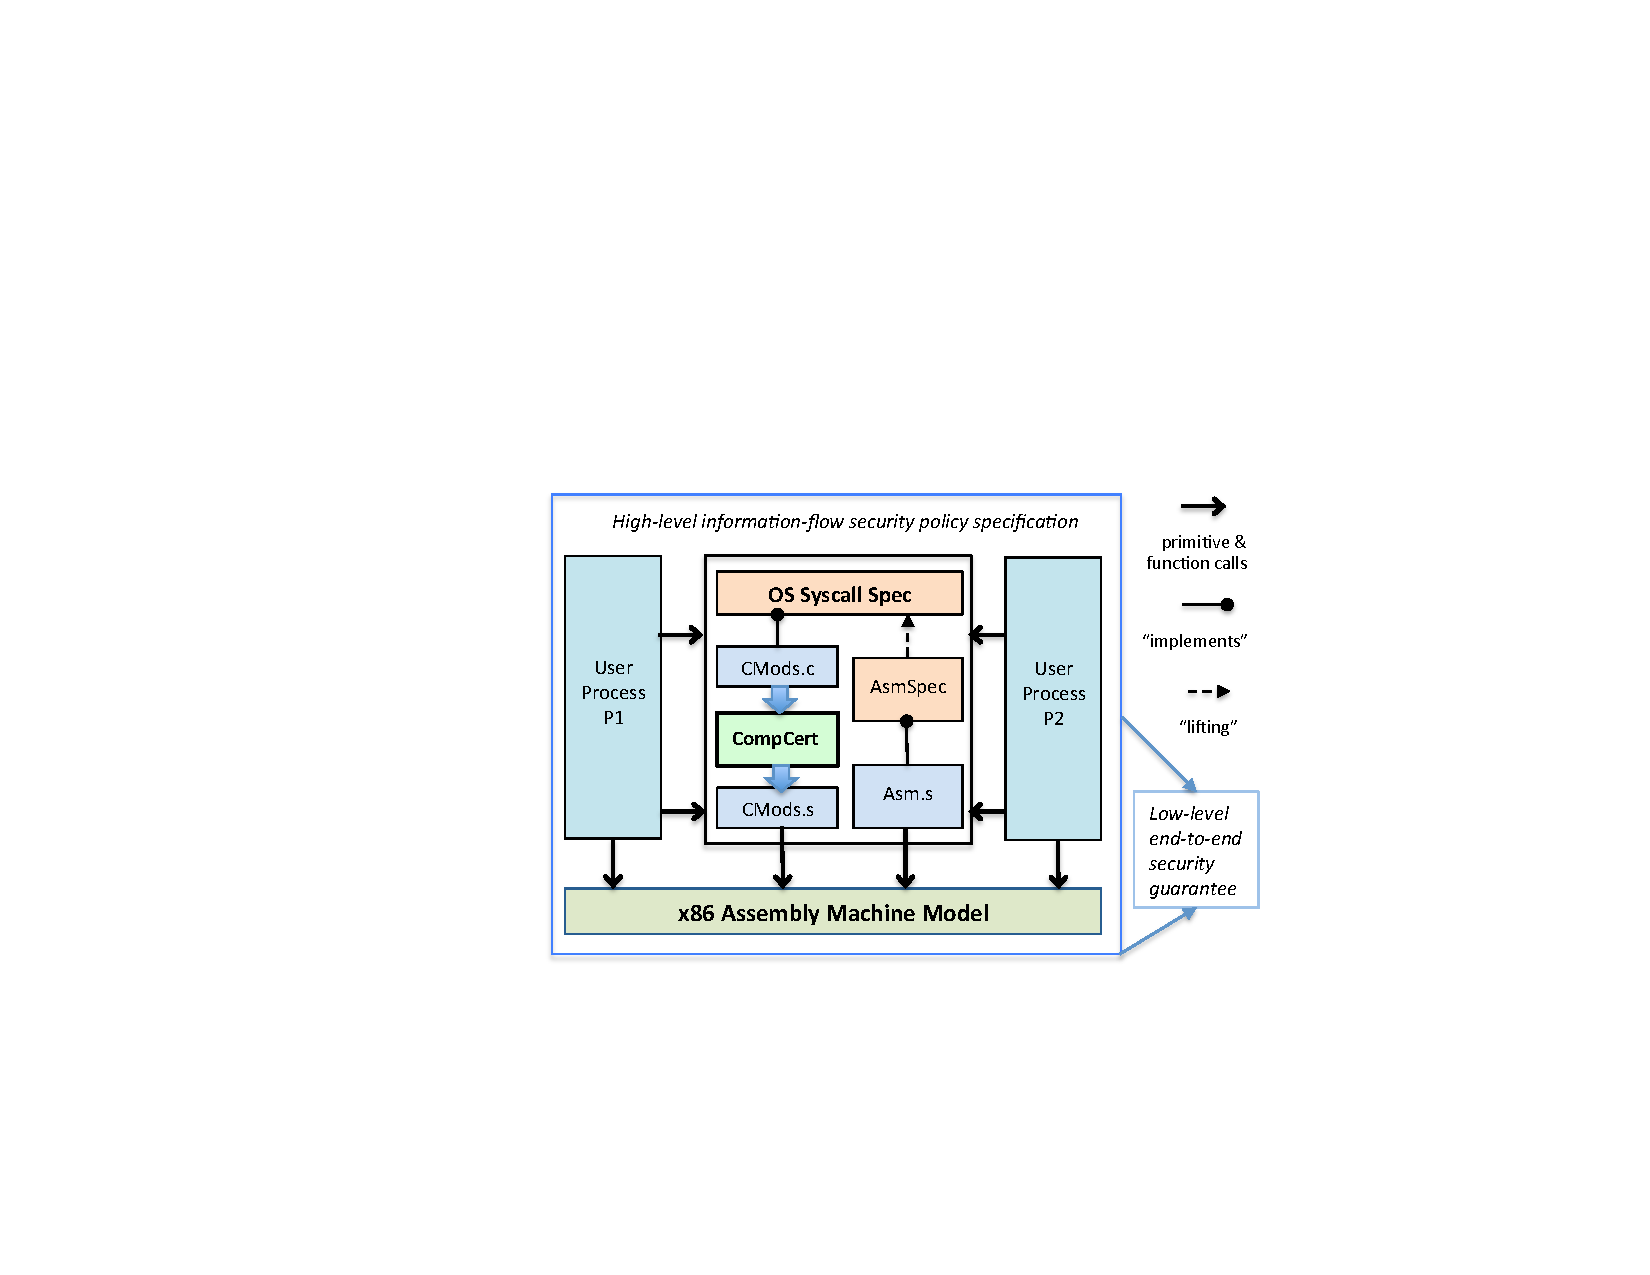
\includegraphics[scale=0.685]{pldi/figure/osmach}
\caption{\small An end-to-end software system that consists 
of both OS modules (in C and assembly) and user processes.}
\label{fig:osmach}
%\vspace*{-20pt}
\end{center}
\end{figure}
%%%%%%%%%%%%%%%%%%%%%%%%%%%%%%%%%%%%%%%%%%%%%%%%%%%%%%%%%%%%%%%%=

Security is desirable in today's real-world software.
Hackers often exploit software bugs to 
obtain information about protected secrets, such as user
passwords or private keys. A formally-verified end-to-end
security proof can guarantee such exploits will never be
successful. There are many significant roadblocks involved
in such a verification, however, and the state-of-the-art
is not entirely satisfactory.
 
Consider the setup of 
Figure~\ref{fig:osmach}, where a large system (e.g., an OS)
consists of many separate functions (e.g., system call primitives) 
written in either C or assembly. Each primitive has a verified
atomic specification, and there is a verified compiler, such as 
CompCert~\cite{compcert}, that can correctly compile C
programs into assembly. We wish to prove an \emph{end-to-end}
security statement about some context program (e.g., P1 or P2) that can call 
the primitives of the system, which ultimately guarantees that 
our model of the concrete execution (i.e., the whole-program assembly 
execution) behaves securely. This goal raises a number of 
challenges:
\begin{itemize}
\item \emph{Policy Specification}~--- How do we specify a clear
and precise security policy, describing how information is
allowed to flow between various domains? If we express the
policy in terms of the high-level syscall specifications, 
then what will this imply for the whole-program assembly execution? 
We need some way of specifying policies at different levels of 
abstraction, as well as translating between or linking separate 
policies.
\item \emph{Propagating Security}~--- It is well 
known~\cite{jurjens,morgan09} that
simulations and refinements may not propagate security guarantees.
How, then, can we soundly obtain a low-level guarantee from a 
high-level security verification?
\item \emph{Proving Security}~--- A standard way to prove
confidentiality is to formulate the property as noninterference,
and prove that some \emph{state indistinguishability} relation is
preserved by each step of execution (this is known as 
an \emph{unwinding condition}~\cite{goguen82,goguen84},
and will be discussed in Section~\ref{informal}). 
% this individual-step property
% is called an \emph{unwinding condition}~\cite{goguen82,goguen84}
% in the literature, and essentially serves as an induction
% hypothesis for proving whole-execution noninterference).
% In our setup, it is natural to express indistinguishability over
% abstract program states, and then prove security by verifying that 
% each primitive specification, taken as an atomic action, preserves
% the relation. 
However, this proof does not propagate down to the 
implementation: a syscall specification may atomically preserve
indistinguishability, but its non-atomic implementation may 
temporarily break the relation during intermediate states. Thus we
must be careful to formulate the security of a primitive's 
implementation as a global behavior-based property over the whole 
execution of the implementation, rather than a local state-based 
property over individual steps.
\item \emph{Cross-Language Linking}~--- Even if we verify security
for all atomic primitive specifications and propagate 
the proofs to implementations, there still may be incompatibilities
between the proofs for C primitives and those for assembly 
primitives. For example, a security proof for an assembly primitive 
might express that some data stored in a particular machine register 
is not leaked; this property cannot be directly chained with one for a 
C primitive since the C memory model does not contain 
machine registers. We therefore must support linking the
specifications of primitives implemented in different languages.
\end{itemize}
%%%%
In this paper, we present a novel methodology
for formally verifying end-to-end security of a system like the one
shown in Figure~\ref{fig:osmach}. First, security is proved for the
high-level specification of each syscall 
in a standard way, establishing noninterference
by showing that a state indistinguishability relation is preserved
across the specification. Then
we apply simulation techniques to automatically obtain a
sound security guarantee for the low-level assembly machine
execution, which is expressed in terms of whole-execution 
observations. Simulations are used both for relating specifications
with their C or assembly implementations, as well as for relating C 
implementations with their compiled assembly implementations.

The central idea of our methodology is to introduce a 
flexible definition of observation that unifies the concepts of 
policy specification, state indistinguishability, and 
whole-execution behaviors. For every level of abstraction, we 
define an \emph{observation function}
that % essentially 
describes which portions of a program state are 
observable to which principals. For
example, an observation function might say that ``$x$ is 
observable to Alice'' and ``$y$ is observable to Bob''.

Different abstraction levels can use different observation functions.
We might use one observation function mentioning machine registers to 
verify an assembly primitive, and a second observation function
mentioning program variables to verify a C primitive. These
observation functions are then linked across abstraction levels via
a special kind of simulation that preserves state
indistinguishability.


\ignore{
The following concepts can be formulated in terms of 
observation functions:
\begin{itemize}
\item \emph{Policy}~--- Given a principal $l$ and program state 
$\sigma$, an observation function induces a security policy
stating that there is no flow of information to $l$ from 
anything in $\sigma$ outside of 
$l$'s observation. In fact, we do not technically require 
observations to be a portion of program state; they can be any
arbitrary transformation on state. This allows us to express a
variety of security policies with % , including some kinds of 
declassification~\cite{sabelfeld-sands}. 
% We will present some examples of interesting 
% policies in Section~\ref{informal}.
\item \emph{Indistinguishability}~--- Two program states are
considered to be indistinguishable to $l$ just when $l$'s observations
on the states are identical.
\item \emph{Whole-Execution Observations}~--- Certain ``well-behaved''
types of observations, such as an append-only output buffer, can be 
used to describe global execution observations, or \emph{behaviors}. 
For example, an execution may have the behavior
``termination with final observation $o$''. We express security of 
the low-level system implementation in terms 
of whole-execution behavioral equality, since the high-level 
unwinding condition does not propagate across simulation.
\item \emph{Linking}~--- We use different observation
functions for different levels of abstraction. This means that we
can use an observation function mentioning machine registers to 
verify an assembly primitive, and a different observation function
mentioning program variables to verify a C primitive. These
observation functions are linked across abstraction levels via
a special kind of simulation that preserves state
indistinguishability.
\end{itemize}
}
%%%%
\begin{comment}
Note that none of these three aspects is individually novel. The
described security proof is a standard method for proving noninterference, 
known as \emph{unwinding}~\cite{goguen82,goguen84}.
The idea of preserving security across simulation or refinement has been 
explored in previous literature, such as~\cite{jurjens,morgan09,murray12}.
Expressing security policies in terms of an abstract notion of
observation or observable equivalence has also been 
explored~\cite{costanzo14,rhtt,sabelfeld99}. Our main contribution
in this work is to unify all three of these aspects with the \emph{single} 
concept of a general observation function. 
\end{comment}
%%%%
We demonstrate the efficacy of our approach by applying it to the mCertiKOS 
operating system~\cite{certikos-popl}. We modify mCertiKOS to disable all 
explicit inter-process communication, and then we prove noninterference between 
user processes with distinct IDs. mCertiKOS guarantees full functional correctness 
of system calls (with respect to an x86 machine model derived from
CompCert's model) by chaining simulations across many abstraction layers. We implement
our general notion of observation function over the existing simulation
framework, and then verify security of the high-level system call 
specifications. The result of this effort is a formally-verified security guarantee 
for the operating system~--- we specify exactly which portions of high-level state 
are observable to which processes, and we prove that the low-level 
model of assembly execution of the whole system is secure with respect to this 
policy. The security guarantee can be seen as \emph{end-to-end} in the following two ways:
(1) it applies across simulations, propagating from a top-level specification to a concrete 
implementation; and (2) it applies to whole-execution behaviors, guaranteeing that an 
entire execution is secure from start to finish. 

\cut{
Note that, while most of the mCertiKOS code is written in C and compiled into
assembly by CompCert, there are some primitives that must be written directly
in assembly. Context switch is a classic example of such a primitive.
The primary functionality of a context switch 
involves copying values between machine registers and kernel objects;
hence both the implementation and specification of the primitive 
must refer to low-level machine state. A key goal and contribution of
our security verification is that assembly primitives like context
switching are fully handled within the framework, and thus do not need to
be trusted.}

\vspace{2mm}
\noindent
To summarize, the primary contributions of this work are:
\begin{itemize}
\item A novel methodology for end-to-end security verification of 
software systems written in both C and assembly, and extending across various
levels of abstraction.
\item An end-to-end security proof, completely formalized in the
Coq proof assistant~\cite{coq}, of a simple but nontrivial operating system
kernel that executes over an extension of the CompCert x86 machine model.
The kernel is non-preemptive, and explicit communication between processes 
is disabled.
\end{itemize}

%\paragraph{Paper Organization}
The rest of this paper is organized as
follows. Sec.~\ref{informal} introduces the
observation function and shows how to use it for policy
specification, security proof, and linking.
Sec.~\ref{methodology} formalizes our simulation framework and
shows how we prove the end-to-end security theorem. 
Sec.~\ref{casestudy-def} and~\ref{casestudy-proof} describe the
security property that we prove over mCertiKOS, 
highlighting the most interesting aspects of our proofs. 
Sec.~\ref{limitations} discusses limitations, assumptions,
and applicability of our methodology. Finally, Sec.~\ref{related}
discusses related work and concludes.

\ignore{


\begin{comment}
The first task took approximately three person-months,
and the second took two person-months.
\end{comment}

\begin{comment}
Consider the setup of Figure~\ref{compile}, where we have an abstract 
specification of a C program, and a compilation of the C program down 
to assembly code. Assume that we have verified two simulations connecting
the specification to the C program, and the C program to the assembly
program.




design a methodology for proving security that
can cleanly support all of the following aspects:
\begin{itemize}
\item \emph{General Policies}~--- It must be easy to define how
state is divided into security domains, how information is allowed
to flow between these domains, and how declassifications can occur.
\item \emph{Application to Low-Level Code}~--- We must have an
end-to-end property that applies to the actual code of the software,
which may be written in C or even assembly.
\item \emph{Tractable Proof Effort}~--- The amount of human effort
required to actually construct the proof must be reasonable.
\end{itemize}
There are many existing frameworks and methodologies for
formally proving security, but none of them satisfactorily
support all of our desired properties. These properties
are often at odds with one another; for example, cleanly
defining security policies requires a high level of abstraction,
and is thus difficult to reconcile with low-level code.

In this work, we will focus on the formal verification
of security for low-level code, such as the C and assembly code that
implements an OS kernel, by leveraging the power of simulation.

We achieve our goal in the following way:
\begin{enumerate}
\item We define security in terms of a highly abstract notion of 
a state observation function. General security policies can be presented 
using this observation function.
\item We define a specialized form of simulation that preserves 
state indistinguishability between machines, as defined by the observation
function. These simulations allow different machines to have different
definitions of observation.
\item We prove that our specialized simulations preserve security: if an
execution of the top-level machine is proved to be secure, then the 
corresponding execution of the bottom-level machine is guaranteed to be secure.
\end{enumerate}
\end{comment}


\begin{comment}
To get a better sense of our approach and its contributions, we will now
discuss how our approach handles two tricky aspects of security verification.

\subsection{Hiding Confidential Data via Atomicity}
\label{hiding}

The following discussion is not novel to our methodology, but rather 
provides some context justifying our choice to prove security at
a high level of abstraction. Let us start with an informal description
of security (confidentiality). Assume we have a type for 
program state and some particular principal (or security domain)
called the \emph{observer}. Our security property will then be 
parameterized by an \emph{observation function} which takes a state 
and returns some part of the state that is known to the observer.
We say that two states are \emph{indistinguishable}, or observably 
equivalent, just when the observations on those states are equal. A 
\emph{secure action} is then a state transition that always takes 
two indistinguishable states to two other indistinguishable states.
Intuitively, secure actions do not leak any information about the
unobservable part of the state. We say that a program is secure
when its semantics, taken as a single big step, constitutes a
secure action.

Note that this definition of security can support some
kinds of declassification policies simply by extending the
observation function. As a very basic example, we can
allow the parity of some high-security data to be declassified
by proving that an action is secure with respect to an observation
function that transforms the high-security data into its
parity. In other words, the action will have the same observable
behavior on any two states in which the high-security data has
the same parity. This semantic and relational view of declassification
is used in some other security-reasoning frameworks such 
as~\cite{sabelfeld99,rhtt,costanzo14}. 

It is trivial to show that secure actions compose sequentially.
This means that we can always prove a program secure by proving
that each individual step of the program is secure. Many existing
security-reasoning frameworks use this strategy. For example,
many typed-based approaches~\cite{jif,hritcu13,slam,austin09} assign security
classifications to program variables (either statically or dynamically),
and then show that each step of the program obeys a policy preventing
information flow from higher classification levels to lower ones.
Some language constructs such as conditional branching must be treated
with care to avoid implicit flows.

This strategy for security verification is unfortunately incomplete,
however, as it necessarily rules out programs that
perform some insecure actions but hide these insecurities
from the observer. As a rather trivial example, the strategy cannot support 
the following simple C program, consisting of an unobservable
global variable~\ttt{password} and an observable global 
variable~\ttt{public}:
\begin{alltt}
  public = password;
  public = 0;
\end{alltt}
This program is atomically secure since it immediately forgets the secret 
data that it read. A line-by-line analysis, however, will not be able
to prove the security of this program since the first line directly
violates security. If an observer reads~\ttt{public} at the point of execution
that occurs in between the two lines of code, then the secret is leaked. 
There are a number of ways to support this type of example, including 
attaching security labels to data instead of locations, and enforcing 
information erasure policies~\cite{chong05}. In this work, we
advocate proving the security of this type of program by abstracting
the program into an atomic specification, and then proving that
the specification is secure.

Note that while this particular example is not something that one would
ever want to write in a real system, we will describe a realistic example
of hiding a potential security leak in
Section~\ref{casestudy-proof}. The example is the implementation of
the page-fault handler in the mCertiKOS kernel. The handler must
allocate a new page and obtain this page's physical address, a value
which could potentially be abused to violate security.  However, the
handler is careful not to make this physical address observable; it is
used only to map the page into the current process's virtual address
space, and then the physical address is forgotten (from the observer's
point-of-view).

While abstracting a program into an atomic action simplifies the security 
proof, it does not solve the whole problem. After all, one of our goals
is that the security proof applies to low-level code~--- the actual
implementation, not the abstract specification. As discussed with the above
example, there is no hope for our security property to hold on each
individual step of the implementation; the steps may be locally insecure. 
Instead, we will prove a global notion of security for the actual 
implementation. While the observation function can refer to any portion
of program state in the abstract specification, we will require that 
implementation uses a different observation function that resembles an
output buffer, or the observer's monitor. More precisely, we will require
a monotonicity property on the observation function of the implementation,
saying that once data is made observable, it can never be made unobservable
later. In the context of the above example, we are essentially saying that
the value of variable \ttt{public} is not what the observer actually sees;
instead, the language should include an explicit print command to 
convert ``observable'' data into ``observed'' data. We will explain and 
formalize this point more clearly in Section~\ref{methodology}. The 
most important thing to see here is that the observation function of the 
specification is \emph{not} required to be monotonic, and can therefore
still express a wide variety of interesting security policies.

\subsection{Security-Preserving Simulation}

Our work represents, to the best of our knowledge, the first disciplined 
approach to preserving security across many layers of simulation. There 
have been other works that addressed the problem of preserving security 
across refinement~\cite{morgan09,jurjens}, including the closely-related
security verification of the seL4 kernel~\cite{murray12}. According
to Lynch's definition~\cite{Lynch95}, a refinement is a special case
of simulation where the simulation relation is a function (i.e., each
state in the higher-level machine is related to exactly one state in
the lower-level machine). Our work aims to preserve security across
arbitrary forward simulations, not just refinements. Indeed, the mCertiKOS
simulations sometimes make use of one-to-many simulation relations
(e.g., abstracting a list into an unordered set).

\begin{figure}
\centering{\includegraphics[scale=0.6,origin=c]{figure/paradox.pdf}}
\caption{\small{Security-Breaking Simulation: both the specification 
and implementation executions are deterministic, yet $R$ causes the 
implementation to be insecure as it relates $y$ to any value.}}
\label{paradox}
\end{figure}

When using refinement, security may not be preserved only when a 
nondeterministic program is refined into a more deterministic one. When 
using general simulations, however, even secure deterministic programs can
be simulated in an insecure way. Figure~\ref{paradox} illustrates this
point. The example assumes a program state consisting of a high-security 
(unobservable) variable $x$ and low-security (observable) variable $y$. 
The abstract action (specification) writes $0$ into $y$, while the concrete 
implementation writes $x$ into $y$. The relation $R$ relating abstract to 
concrete states simply requires that $x$ has the same value in the two 
states, and $y$ always has value $0$ in the abstract state (hence the
relation is one-to-many). It is easy to show that $R$ is a valid simulation
relation for this example (in fact, it is a valid bisimulation
relation). The abstract action is clearly secure,
as the final value of $y$ is guaranteed to be $0$ and thus has no 
dependency on the secret value of $x$. However, the implementation
is not secure: the final value of $y$ clearly depends directly
on $x$. Using the terminology above, the state observation is the value
of $y$; the abstract program always takes two indistinguishable initial 
states to indistinguishable final states, while the concrete one may not.

Our solution to this issue is obvious but fundamental. The simulation in
Figure~\ref{paradox} breaks security because security talks about 
indistinguishability of states, yet the relation $R$ fails to 
preserve indistinguishability. We therefore define a notion of
``indistinguishability-preserving simulation'', which is a normal
simulation with the additional property that two indistinguishable
states are always related to indistinguishable states. We will formalize
this in Section~\ref{methodology}, and prove that such a simulation
preserves security.

%\vspace{2mm}
\noindent
To summarize, the contributions of our work are as follows:
\begin{itemize}
\item We present a novel methodology for proving security based on
layered simulations. The security proof is done at the most
abstract layer, and can therefore express interesting policies,
including some kinds of declassification. The simulations are
specialized to preserve security, so that an
end-to-end property still holds over the most concrete layer.
No security reasoning is required over any layer besides the
abstract one.
\item We demonstrate the effectiveness of this methodology with
a major proof effort: the confidentiality between user-processes
executing over the mCertiKOS~\cite{certikos-popl} kernel.
Like mCertiKOS, our proof is fully formalized in the Coq proof 
assistant~\cite{coq}, and the code can be found in the supplementary
material~\cite{costanzo-popl16-tr}.
\end{itemize}
\end{comment}

\begin{comment}
Now that we have described our methodology for proving security,
let us revisit the initial goals:
\begin{itemize}
\item \emph{General Policies}~--- 
The observation function allows us to specify interesting security 
policies at an arbitrarily high level of abstraction. We will 
present many example policies in Section~\ref{policies}. 
\item \emph{Application to Low-Level Code}~--- 
Our solution to the refinement paradox (restricting the simulation
relation according to observations)
allows us to propagate a high-level security policy to the actual 
low-level execution.
\item \emph{Tractable Proof Effort}~--- The required proof effort is 
reasonable, as it is divided into the two
orthogonal tasks of abstracting code into a functional specification, and
then proving security over the specification. The security proof only
requires showing that single steps preserve observable equivalence;
multi-step reasoning follows automatically from induction.  
Functional specifications can be reused for proving other properties 
besides security. In Sections~\ref{casestudy-def} and~\ref{casestudy-proof}, 
we support our claim 
that the proof effort is reasonable by presenting a full security proof 
over a variant of the mCertiKOS kernel.
\item \emph{Completeness}~--- Our proof strategy achieves a satisfactory 
level of completeness, since it allows for proving an entire program secure 
even when the program manipulates data in a locally insecure way.
\end{itemize}
\end{comment}

\begin{comment}
\subsection{Security Verification of mCertiKOS}

In Sections~\ref{casestudy-def} and~\ref{casestudy-proof}, we
demonstrate our security proof methodology with a large-scale,
practical example. We prove a security property over a version of the
mCertiKOS kernel, stating that user processes are isolated from each
other. The proof is developed entirely within the Coq proof assistant,
and thus is machine-checkable.

The first step of the proof~--- abstraction of system call
implementations into functional specifications~--- was already
completed by Gu~{\em et al}~\cite{certikos-popl}. The proof presented
here deals with the second step: specifying a security policy
(observation function) and proving the security property instantiated
with this policy. While the abstraction step took about $1.5$
person-years (including the time for developing much of the refinement
framework), the security step took only $3$ person-months to complete.

To the best of our knowledge, our work is only the second
fully-formalized OS security proof to be completed; the first is the
verification effort over the seL4 
kernel~\cite{klein14,sewell11,murray12,murray13}.
There are some major shortcomings in the seL4 effort, however, that
our methodology allows us to address. One shortcoming comes from the
fact that the seL4 proof uses standard refinement rather than
contextual refinement.  This means that malicious user code (context
code) could potentially interfere with kernel state in such a way that
the refinement becomes unsound. Indeed, the seL4 security proof needs
to assume that user-level actions only touch a portion of memory state
isolated from the kernel (the user's virtual address space). In our
security verification over mCertiKOS, we \emph{prove} that users'
actions are correctly isolated to their virtual address spaces.

A second shortcoming of the seL4 proof is that it does not deal with
page faults in their model of user-level
transitions~\cite{klein14,daum14}; this is a severe limitation since
virtual memory without page fault handling would be almost unusable.
As we will show later in Section~\ref{ssec:oprim}, the security of the
page-fault handling primitive is one of the hardest and the most
tricky components in our security verification over mCertiKOS.

A third shortcoming of the seL4 proof is that their state simulation
relation is the identity relation. This means that, while they can abstract
code into atomic specifications, they cannot abstract machine state 
into more convenient forms or into purely logical state. Not only
does this make the functional specifications difficult to present
in a readable way, but it also limits the expressiveness of security 
policies. Note that they completely elide the refinement
paradox issue by never abstracting program state.

A fourth issue with the seL4 proof is that refinement is only verified
for implementations written in C. Anything written directly in
assembly is assumed to have been implemented and abstracted correctly.
This is particularly relevant for an operating system, since there is
some functionality such as context switching that \emph{must} be
implemented in assembly. Our contextual refinement framework, on the
other hand, guarantees that the functional specification is a correct
abstraction of the actual implementation, regardless of whether the
implementation is written in C or assembly. Thus we can be certain
that our security theorem propagates down to the actual
implementation, even across assembly primitives like context switch.
\end{comment}

}


\chapter{Locality and Behavior Preservation}
\label{bpsl-chapter}

In this chapter, we present our work published in 
APLAS~2012~\cite{costanzo-bpsl}. In the context of 
Separation Logic~\cite{io00,reynolds02,yang:fossacs02,coy07},
we define and defend a strong notion of locality, deemed
``behavior preservation''. Locality concerns the relationship
between a program's execution over a small footprint state
and its execution over a larger state containing unused
resources. Our key idea is to require a behavior-preserving
formulation of locality, where the program's behavior is
completely unchanged by the extra unused resources.

We describe here (and in the paper) how behavior preservation
simplifies numerous metatheoretical difficulties in Separation Logic.
This is mostly orthogonal to the rest of the dissertation, as it does
not concern security. However, we will discuss some interesting
connections to security at the end of the chapter, by
relating behavior preservation with classical noninterference.

\section{Local Reasoning and the Frame Rule}
\label{locality}

Separation Logic is a program logic that allows for formal
reasoning about the behavior of heap-manipulating C-like 
programs. The most important concept is the 
\emph{separating conjunction}~--- the assertion $P*Q$ holds
on a program state if that state can be separated into 
two \emph{disjoint} portions, one satisfying $P$ and the
other satisfying $Q$. The following \emph{frame rule} is
used to facilitate local reasoning:
\begin{mathpar}
\inferrule
{\judg{}{P}{C}{Q}}
{\judg{}{P * R}{C}{Q * R}}
\end{mathpar}
\noindent{}That is, if a program $C$ is verified to satisfy
a pre/post condition pair $(P,Q)$, then we can automatically 
infer that it also satisfies the pair $(P*R,Q*R)$, where
$R$ describes program state that is disjoint from both
$P$ and $Q$. Intuitively, this seems to indicate that the 
unused resources in $R$ do not affect $C$'s behavior.
Formally, however, the notion of locality required by the
frame rule is actually weaker than this intuition. There
are three locality-related properties that together imply 
soundness of the frame rule, commonly called Safety Monotonicity,
the Frame Property, and Termination Monotonicity (the
latter is only needed for termination-sensitive reasoning).

\begin{comment}
In standard Separation
Logic~\cite{io00,reynolds02,yang:fossacs02,coy07}, there are two
locality properties, known as Safety Monotonicity and the Frame
Property, that together imply soundness of the frame rule.  Safety
Monotonicity says that any time a program executes safely in a certain
state, the same program must also execute safely in any larger
state~--- in other words, unused resources cannot cause a program to
crash. The Frame Property says that if a program executes safely on a
small state, then any terminating execution of the program on a larger
state can be tracked back to some terminating execution on the small
state by assuming that the extra added state has no effect and is
unchanged. Furthermore, there is a third property, called Termination
Monotonicity, that is required whenever we are interested in reasoning
about divergence (nontermination).  This property says that if a
program executes safely and never diverges on a small state, then it
cannot diverge on any larger state.
\end{comment}

To describe these properties more formally, we first 
introduce some notations for combining disjoint program states. 
%We will describe the theory
%somewhat informally here; full formal detail will be described later
%in Section~\ref{abslogic}. 
We define states $\sigma$ to be members of
an abstract set $\Sigma$. We assume that whenever two states
$\sigma_0$ and $\sigma_1$ are ``disjoint,'' written $\sigma_0 \#
\sigma_1$, they can be combined to form the larger state $\sigma_0 \dt
\sigma_1$. Intuitively, two states are disjoint when their heaps occupy
disjoint areas of memory.

We represent the semantic meaning of a program $C$ by a binary
relation $\den{C}$, indicating all possible whole-execution behaviors
of $C$. We use the common notational convention
$\relate{R}{a}{b}$ for a binary relation $R$ to denote $(a,b) \in
R$. Intuitively, $\relate{\den{C}}{\sigma}{\sigma'}$ means that, when
executing $C$ on initial state $\sigma$, it is possible to terminate
in state $\sigma'$.  Note that if $\sigma$ is related by $\den{C}$ to
more than one state, this simply means that $C$ is a nondeterministic
program.
We also define two special behaviors $\fault$ and $\dvg$:
\begin{itemize}
\item $\relate{\den{C}}{\sigma}{\fault}$ means that $C$ can crash or get
stuck when executed on $\sigma$
\item $\relate{\den{C}}{\sigma}{\dvg}$ means that $C$ can diverge (execute
forever) when executed on $\sigma$
\end{itemize}

As a notational convention, we use $\tau$ to range over elements of
$\Sigma \cup \{\fault,\dvg\}$. We require that for any state $\sigma$
and program $C$, there is always at least one $\tau$ such that
$\relate{\den{C}}{\sigma}{\tau}$. In other words, every execution must
either crash, go on forever, or terminate in some state.

Now we define the properties mentioned above. Following are definitions of
Safety Monotonicity, the Frame Property, and Termination Monotonicity, respectively
(when not explicitly mentioned, assume all variables are universally quantified):
\begin{align*}
& \text{1.) }\ \lnot \relate{\den{C}}{\sigma_0}{\fault} \land \sigma_0 \# \sigma_1 \Longrightarrow 
  \lnot \relate{\den{C}}{(\sigma_0 \dt \sigma_1)}{\fault} \\ 
& \text{2.) }\ \lnot \relate{\den{C}}{\sigma_0}{\fault} \land \relate{\den{C}}{(\sigma_0 \dt \sigma_1)}{\sigma'} \Longrightarrow \exists \sigma_0' \such \sigma' = \sigma_0' \dt \sigma_1 \land \relate{\den{C}}{\sigma_0}{\sigma_0'} \\
& \text{3.) }\ \lnot \relate{\den{C}}{\sigma_0}{\fault} \land \lnot \relate{\den{C}}{\sigma_0}{\dvg} 
  \land \sigma_0 \# \sigma_1
\Longrightarrow \lnot \relate{\den{C}}{(\sigma_0 \dt \sigma_1)}{\dvg}\end{align*}
\noindent{}Safety Monotonicity says that any time a program executes safely 
in a certain state, the same program must also execute safely in any larger
state~--- in other words, unused resources cannot cause a program to
crash. The Frame Property says that if a program executes safely on a
small state, then any terminating execution of the program on a larger
state can be tracked back to some terminating execution on the small
state by assuming that the extra added state has no effect and is
unchanged. Termination Monotonicity says that if a
program executes safely and never diverges on a small state, then it
cannot diverge on any larger state.

In standard Separation Logic, these three properties are required to
hold for all programs $C$, and the frame rule is then automatically
guaranteed to be sound. The properties represent 
the \emph{minimum} requirement needed to make the frame rule sound~--- they
are as weak as they can possibly be without breaking the logic. They are
not defined to correspond with any intuitive notion of locality. As a
result, there are two subtleties in the definition that might seem a
bit odd. We will now describe these subtleties and the changes we make
to get rid of them. Note that we are not arguing in this section that
there is any benefit to changing locality in this way (other than the
arguably vacuous benefit of corresponding to our ``intuition'' of
locality)~--- the benefit will become clear when we discuss how our
change simplifies the metatheory in Section~\ref{metatheory}.

The first subtlety is that Termination Monotonicity only applies in
one direction. This means that we could have a program $C$ that runs
forever on a state $\sigma$, but when we add unused state, we suddenly
lose the ability for that infinite execution to occur. We can easily
get rid of this subtlety by replacing Termination Monoticity with the
following Termination Equivalence property:
{\small
\begin{align*}
\lnot \relate{& \den{C}}{\sigma_0}{\fault} \land \sigma_0 \# \sigma_1 \Longrightarrow
  (\relate{\den{C}}{\sigma_0}{\dvg} \iff \relate{\den{C}}{(\sigma_0 \dt \sigma_1)}{\dvg})
\end{align*}}
\indent{}The second subtlety is that locality gives us a way of tracking an execution on a large state 
back to a small one, but it does not allow for the other way around. This means that there
can be an execution on a state $\sigma$ that becomes invalid when we add unused state. This 
subtlety is a little trickier to remedy than the other. If we think of the Frame Property as
really being a ``Backwards Frame Property,'' in the sense that it only works in the direction
from large state to small state, then we clearly need to require a corresponding Forwards
Frame Property. We would like to say that if $C$ takes $\sigma_0$ to $\sigma_0'$ and we add 
the unused state $\sigma_1$, then $C$ takes $\sigma_0 \dt \sigma_1$ to $\sigma_0' \dt \sigma_1$:
{\small
\begin{align*}
\relate{\den{C}}{\sigma_0}{\sigma_0'} \land \sigma_0 \# \sigma_1 \Longrightarrow 
  \relate{\den{C}}{(\sigma_0 \dt \sigma_1)}{(\sigma_0' \dt \sigma_1)}
\end{align*}}
\indent{}Unfortunately, there is no guarantee that $\sigma_0' \dt \sigma_1$ is defined, as the
states might not occupy disjoint areas of memory. In fact, if $C$ causes our initial state
to grow, say by allocating memory, then there will always be some $\sigma_1$ that is 
disjoint from $\sigma_0$ but not from $\sigma_0'$ (e.g., take $\sigma_1$ to be exactly that
allocated memory). Therefore, it seems as if we are doomed to lose behavior in such a situation
upon adding unused state.

There is, however, a solution worth considering: we could disallow programs from ever increasing state.
In other words, we can require that whenever $C$ takes $\sigma_0$ to $\sigma_0'$, the area of
memory occupied by $\sigma_0'$ must be a subset of that occupied by $\sigma_0$. In this way,
anything that is disjoint from $\sigma_0$ must also be disjoint from $\sigma_0'$, so we
will not lose any behavior. Formally, we express this property as:
{\small\begin{align*}
\relate{\den{C}}{\sigma_0}{\sigma_0'} \Longrightarrow (\forall \sigma_1 \such \sigma_0 \# \sigma_1 \Rightarrow \sigma_0' \# \sigma_1)
\end{align*}}
\indent{}We can conveniently combine this property with the previous one to express
the Forwards Frame Property as the following condition:
{\small
\begin{align*}
\relate{\den{C}}{\sigma_0}{\sigma_0'} \land \sigma_0 \# \sigma_1 \Longrightarrow 
  \sigma_0' \# \sigma_1 \land \relate{\den{C}}{(\sigma_0 \dt \sigma_1)}{(\sigma_0' \dt \sigma_1)}
\end{align*}}
\indent{}At first glance, it may seem imprudent to impose this requirement,
as it apparently disallows memory allocation. However, it is in fact still possible to model 
memory allocation~--- we just have to be a little clever about it. Specifically, we can include
a set of memory locations in our state that we designate to be the ``free list''. When memory
is allocated, all allocated cells must be taken from the free list. Because the free list
is represented explicitly in program state, any extra unused resources must be disjoint
not only from the heap, but also from the free list. Contrast this to standard 
Separation Logic, in which newly-allocated heap cells are taken from outside the program 
state. In the next section, we will show that we can add a free list in this way to the 
model of Separation Logic without requiring a change to any of the inference rules.

We conclude this section with a brief justification of the term ``behavior preservation.''
Given that $C$ runs safely on a state $\sigma_0$, we think of a behavior of $C$ on $\sigma_0$ as
a particular execution, which can either diverge or terminate at some state $\sigma_0'$. 
The Forwards Frame Property tells us that execution on a larger state $\sigma_0 \dt \sigma_1$
simulates execution on the smaller state $\sigma_0$, while the Backwards (standard) Frame Property
says that execution on the smaller state simulates execution on the larger one. Since standard locality
only requires simulation in one direction, it is possible for a program to have fewer valid executions, or 
behaviors, when executing on $\sigma_0 \dt \sigma_1$ as opposed to just $\sigma_0$. Our stronger
locality disallows this from happening, enforcing a \emph{bisimulation} under which all 
behaviors (including divergence) are preserved when extra resources are added.

\section{Impact on a Concrete Separation Logic}
\label{concrete}

In this section, we will demonstrate how behavior-preserving
locality can be enforced in a standard model of Separation Logic
without any negative impact on using the program logic. In the 
standard Reynolds' Separation Logic model~\cite{reynolds02}, a program state
consists of two components: a variable store and a heap. When new
memory is allocated, the memory is taken from outside the state
and added into the heap. As mentioned in Section~\ref{locality}, this
notion of memory allocation violates our Forwards Frame Property,
so we will instead include an
explicit free list inside the program state. Thus a state is now is a
triple $(s,h,f)$ consisting of a store, a heap, and a free list, with
the heap and free list occupying disjoint areas of
memory. Newly-allocated memory always comes from the free list,
while deallocated memory goes back into the free list. Since the
standard formulation of Separation Logic assumes that memory is
infinite and hence that allocation never fails, we similarly require
the free list to be infinite. More specifically, we require that
there is some location $n$ such that all locations above $n$ are in
the free list.
Formally, states are defined as follows:
{\small
\begin{align*}
& \text{Var } V \isdef \{x,y,z,\ldots \} \qquad \text{Store } S \isdef V \to \Z \qquad \text{Heap } H \isdef \N \finpf \Z \\
& \text{Free List } F \isdef \{N \in \pwrset{\N} \pipe \exists n \such \forall k \geq n \such k \in N\} \\
& \text{State } \Sigma \isdef \{(s,h,f) \in S \times H \times F \pipe \text{dom}(h) \cap f = \emp\}
\end{align*}
}
\indent{}As a point of clarification, we are not claiming here that including the free list in 
the state model is a novel idea. Other systems (e.g.,~\cite{rg09}) have made use of a 
very similar idea. The two novel contributions that we will show in this section are:
(1) that a state model which includes an explicit free list can provide a behavior-preserving
semantics, and (2) that the corresponding program logic can be made to be completely 
backwards-compatible with standard Separation Logic (meaning that any valid Separation 
Logic derivation is also a valid derivation in our logic).

%%%%%%%%%%%%%%%%%%%%%%%%%%%%%%%%%%%%%%%%%%%%%%%%%%%%%%%%%%%%%%%%%%%%%%%%%%%%
\begin{figure}[t]
\begin{mathpar}

\hspace{-15mm}    
\begin{bnf}[r@{\ \ \ }c@{\ }]

\production{& E}
    \prodcase{E + E'}
    \prodcase{E - E'}
    \prodcase{\ldots}
    \prodcase{-1}
    \prodcase{0}
    \prodcase{1}
    \prodcase{\ldots}
    \prodcase{x}
    \prodcase{y}
    \prodcase{\ldots}
    
\production{& B}
    \prodcase{E=E'}
    \prodcase{\false}
    \prodcase{B \Rightarrow B'}
    
\production{& P,Q}
    \prodcase{B}
    \prodcase{\false}
    \prodcase{\empa}
    \prodcase{E \mapsto E'}
    \prodcase{P \Rightarrow Q}
    \prodcase{P*Q}
    
\production{& C}
    \prodcase{\skp}
    \prodcase{x:=E}
    \prodcase{x:=[E]}
    \prodcase{[E]:=E'}
    \prodcase{x:=\cons(E_1,\ldots,E_n)}
    \prodcase{\free(E)}
    \prodcase{C;C'}
    \prodcase{\condfull{B}{C}{C'}}
    \prodcase{\while{B}{C}}
    
\end{bnf}
\end{mathpar}

\caption{Assertion and Program Syntax}
\label{syntax}
\end{figure}

%%%%%%%%%%%%%%%%%%%%%%%%%%%%%%%%%%%%%%%%%%%%%%%%%%%%%%%%%%%%%%%%%%%%%%%%%%%%

\ifextended
We adopt the following standard notations: $\dom{h}$ is the domain of the heap $h$;
$s[x \mapsto v]$ is the store which is identical to $s$, except that the value of variable $x$
is updated to $v$; $h[l \mapsto v]$ is the heap which is identical to $h$, except that location
$l$ is either added to $h$ with value $v$ if it does not exist in $h$, or updated with value $v$
if it does exist; $h \backslash l$ is the heap resulting from removing location $l$ from $h$;
$h_0 \# h_1$ is true just when $\dom{h_0}$ and $\dom{h_1}$ do not overlap;
$h_0 \dt h_1$ is equal to the union of $h_0$ and $h_1$ if $h_0 \# h_1$, and is undefined otherwise.
We also overload the disjointness (\#) operator to work with free lists~--- e.g., $h \# f$ says 
that $\dom{h}$ and $f$ are disjoint.
\fi

Assertion syntax and program syntax are given in Figure~\ref{syntax}, and are exactly
the same as in the standard model for Separation Logic. 
\ifextended
This syntax includes expressions
$E$ and boolean expressions $B$, both of which can be evaluated under a given variable store,
without any knowledge of the heap. These valuations are denoted by $\den{E}s$ and $\den{B}s$ 
for a given store $s$; the former
evaluates to an integer, while the latter evaluates to a boolean. Their formal definitions
are omitted here, but are straightforward and standard in the literature.
\fi

Our satisfaction judgement $(s,h,f) \models P$ for an assertion $P$ is
defined by ignoring the free list and only considering whether $(s,h)$
satisfies $P$. The definition of $(s,h)~\models~P$ is identical to
that of standard Separation Logic, and is given in Figure~\ref{satisfaction}.
The most important cases are $E \mapsto E'$ and $P*Q$. $E
\mapsto E'$ says that the current heap consists \emph{only} of the
memory cell at address $\den{E}s$, and that the cell at that address
maps to the value $\den{E'}s$. $P*Q$ says that we can separate the
current heap into two disjoint subheaps $h_0$ and $h_1$, with $h_0$
satisfying $P$ and $h_1$ satisfying $Q$. We also define the standard
syntactic sugars $E \mapsto E_0,\ldots,E_n$ to be $(E \mapsto E_0) *
\ldots * (E+n \mapsto E_n)$, and $E \mapsto -$ to be $\exists x . E
\mapsto x$ (where $x$ is not free in $E$).

\begin{figure}[t]

\begin{align*}
(s,h) \models B & \iff \den{B}s = \true \\
(s,h) \models \false & \iff \text{never} \\
(s,h) \models \empa & \iff \dom{h} = \emptyset \\
(s,h) \models E \mapsto E' & \iff \dom{h} = \{\den{E}s\} \land h(\den{E}s) = \den{E'}s \\
(s,h) \models P \Rightarrow Q & \iff \text{if } (s,h) \models P \text{, then } (s,h) \models Q \\
%%%%%%%%%%%%%%%%%%%%%%%%%%%%%%%%%
(s,h) \models P*Q & \iff 
\left(\begin{aligned}
\exists & h_0, h_1 \such h_0 \# h_1 \land h_0 \dt h_1 = h \hspace{1mm} \land \\
& (s,h_0) \models P \land (s,h_1) \models Q
\end{aligned}\right)
%%%%%%%%%%%%%%%%%%%%%%%%%%%%%%%%%
\end{align*}

\caption{Satisfaction of Assertions}
\label{satisfaction}
\end{figure}

%%%%%%%%%%%%%%%%%%%%%%%%%%%%%%%%%%%%%%%%%%%%%%%%%%%%%%%%%%%%%%%%%%%%%%%%%%%%

\ifextended

Figure~\ref{opsem} defines the small-step operational semantics for our 
machine. $x:=[E]$ and
$[E]:=E'$ correspond to reading from and writing to the heap, respectively. $x:=\cons(E_1,\ldots,E_n)$
allocates a nondeterministically-chosen contiguous block of $n$ heap cells from the free list.
The most interesting rules are those for allocation and deallocation, since they make use of the free list. 
Note that none of the operations make use of any memory existing outside the program state~---
this is the key for obtaining behavior-preservation.

\begin{figure*}

\begin{mathpar}
\inferrule*[right=(SKIP)]
{\hspace{1mm}}
{\sigma,\skp;C \bpstep \sigma,C}

\inferrule*[right=(ASSGN)]
{\hspace{1mm}}
{(s,h,f),x:=E \bpstep (s[x \mapsto \den{E}s],h,f),\skp}

\inferrule*[right=(HEAP-READ)]
{\den{E}s \in \dom{h}}
{(s,h,f),x:=[E] \bpstep (s[x \mapsto h(\den{E}s)],h,f),\skp}

\inferrule*[right=(HEAP-WRITE)]
{\den{E}s \in \dom{h}}
{(s,h,f),[E]:=E' \bpstep (s,h[\den{E}s \mapsto \den{E'}s],f),\skp}

\inferrule*[right=(CONS)]
{\forall i \in [1,n] \such l+i-1 \in f}
{(s,h,f),x:=\cons(E_1,\ldots,E_n) \bpstep \\
(s[x \mapsto l], h[l \mapsto \den{E_1}s]\ldots[l+n-1 \mapsto \den{E_n}s], f-\{l,\ldots,l+n-1\}),\skp}

\inferrule*[right=(FREE)]
{\den{E}s \in \dom{h}}
{(s,h,f),\free(E) \bpstep (s,h \backslash \den{E}s,f \cup \{\den{E}s\}),\skp}

\inferrule*[right=(SEQ)]
{\sigma,C \bpstep \sigma',C'}
{\sigma,C;C'' \bpstep \sigma',C';C''}

\inferrule*[right=(IF-TRUE)]
{\den{B}s = \texttt{true}}
{\sigma,\condfull{B}{C_1}{C_2} \bpstep \sigma,C_1}

\inferrule*[right=(IF-FALSE)]
{\den{B}s = \texttt{false}}
{\sigma,\condfull{B}{C_1}{C_2} \bpstep \sigma,C_2}

\inferrule*[right=(WHILE-TRUE)]
{\den{B}s = \texttt{true}}
{\sigma,\while{B}{C} \bpstep \sigma,C;\while{B}{C}}

\inferrule*[right=(WHILE-FALSE)]
{\den{B}s = \texttt{false}}
{\sigma,\while{B}{C} \bpstep \sigma,\skp}
\end{mathpar}

\caption{Small-Step Operational Semantics}
\label{opsem}
\end{figure*}

\else

The small-step operational semantics for our machine is defined as
$\sigma,C \bpstep \sigma',C'$ and is straightforward; the full details can
be found in the extended TR. The most interesting aspects are the rules 
for allocation and deallocation, since they make use of the free list.
$x:=\cons(E_1,\ldots,E_n)$ allocates a nondeterministically-chosen
contiguous block of $n$ heap cells from the free list, while $\free(E)$
puts the single heap cell pointed to by $E$ back onto the free list.
None of the operations make use of any memory existing outside the program 
state~--- this is the key for obtaining behavior-preservation.
\fi

To see how out state model fits into the structure defined in Section~\ref{locality},
we need to define the state combination operator. Given two states $\sigma_1 = (s_1,h_1,f_1)$ and
$\sigma_2 = (s_2,h_2,f_2)$, the combined state $\sigma_1 \dt \sigma_2$ is equal to 
$(s_1,h_1 \uplus h_2,f_1)$ if $s_1 = s_2$, $f_1 = f_2$, and the domains of $h_1$ and $h_2$ are
disjoint; otherwise, the combination is undefined. Note that this combined state satisfies the
requisite condition $\text{dom}(h_1 \uplus h_2) \cap f_1 = \emp$ because $h_1$, $h_2$, and $f_1$
are pairwise disjoint by assumption. The most important aspect of this definition of state 
combination is that we can never change the free list when adding extra resources. This guarantees
behavior preservation of the nondeterministic memory allocator because the allocator's set of 
possible behaviors is precisely defined by the free list.

In order to formally compare our logic to standard Separation Logic, we 
need to provide the standard version of the small-step operational semantics,
denoted as $(s,h),C \istep (s',h'),C'$. This definition is nearly identical
to Figure~\ref{opsem}, except that all free lists are removed from program
state, and the (CONS) rule precondition is modified to only require that
the newly-allocated locations are not in $\dom{h}$.
\ifextended
It is then possible to show the following relationship between the
two operational semantics (note that the full proofs for all of the following 
lemmas and theorems can be found in our Coq implementation~\cite{costanzo-thesis}):

\begin{lem}
\label{opequiv}
\begin{align*}
(s,h),C \istepn{n} & (s',h'),C' \iff \exists f,f' \such (s,h,f),C \bpstepn{n} (s',h',f'),C'
\end{align*}
\end{lem}
\else
We formalize this semantics in the extended TR, and prove the following relationship between the
two operational semantics:
{\small
\begin{align*}
(s,h),C \istepn{n} & (s',h'),C' \iff \exists f,f' \such (s,h,f),C \bpstepn{n} (s',h',f'),C'
\end{align*}}
\fi
\ifextended
\begin{proof}
The backwards direction is a straightforward proof by induction. For the forwards direction, we actually
prove a stronger statement by picking our $f$ and $f'$ to be exactly $\N-\dom{h}$ and $\N-\dom{h'}$,
respectively. The proof of this stronger statement is then straightforward by induction. Picking the free
lists in this way showcases how the Separation Logic model can be interpreted as having an implicit free list
containing everything not in the heap.
\end{proof}

\fi
\ifextended
The inference rules in the form $\assertd{P}{C}{Q}$ for our logic
are exactly the same as those used in standard Separation Logic.
We give many of these inference rules in Figure~\ref{infrules}; the
reader may refer to \cite{reynolds02} for more.
%%
%%%%%%%%%%%%%%%%%%%%%%%%%%%%%%%%%%%%%%%%%%%%%%%%%%%%%%%%%%%%%%%%%%%%%%%%%%%%
\begin{figure}
\begin{mathpar}
\inferrule*[right=(SKIP)]
{\hspace{1mm}}
{\assertd{\empa}{\skp}{\empa}}
%
~~~
\inferrule*[right=(ASSGN)]
{\hspace{1mm}}
{\assertd{x=y \land \empa}{x:=E}{x=E\sub{y}{x} \land \empa}}

\inferrule*[right=(HEAP-READ)]
{\hspace{1mm}}
{\assertd{x=y \land E \mapsto z}{x:=[E]}{x=z \land E\sub{y}{x} \mapsto z}}

\inferrule*[right=(HEAP-WRITE)]
{\hspace{1mm}}
{\assertd{E \mapsto -}{[E]:=E'}{E \mapsto E'}}

\inferrule*[right=(CONS)]
{\hspace{1mm}}
{\assertd{x=y \land \empa}{x:=\cons(E_1,\ldots,E_k)}{x \mapsto E_1\sub{y}{x},\ldots,E_k\sub{y}{x}}}

\inferrule*[right=(FREE)]
{\hspace{1mm}}
{\assertd{E \mapsto -}{\free(E)}{\empa}}

\inferrule*[right=(SEQ)]
{\assertd{P}{C_1}{Q} \\
\assertd{Q}{C_2}{R}}
{\assertd{P}{C_1;C_2}{R}}

\inferrule*[right=(IF)]
{\assertd{B \land P}{C_1}{Q} \\
\assertd{\lnot B \land P}{C_2}{Q}}
{\assertd{P}{\condfull{B}{C_1}{C_2}}{Q}}

\inferrule*[right=(WHILE)]
{\assertd{B \land P}{C}{P}}
{\assertd{P}{\while{B}{C}}{\lnot B \land P}}

\inferrule*[right=(CONSEQ)]
{P' \Rightarrow P \\
Q \Rightarrow Q' \\
\assertd{P}{C}{Q}}
{\assertd{P'}{C}{Q'}}

\inferrule*[right=(CONJ)]
{\assertd{P_1}{C}{Q_1} \\
\assertd{P_2}{C}{Q_2}}
{\assertd{P_1 \land P_2}{C}{Q_1 \land Q_2}}

\inferrule*[right=(DISJ)]
{\assertd{P_1}{C}{Q_1} \\
\assertd{P_2}{C}{Q_2}}
{\assertd{P_1 \lor P_2}{C}{Q_1 \lor Q_2}}

\inferrule*[right=(FRAME)]
{\assertd{P}{C}{Q} \\
\texttt{modifies}(C) \cap \texttt{vars}(R) = \emp}
{\assertd{P*R}{C}{Q*R}}
\end{mathpar}
%%%%%%%%%%%%%%%%%%%%%%%%%%%%%%%%%%%%%%%%%%%%%%%%%%%%%%%%%%%%%%%%%%%%%%%%%%%%
\caption{Some Separation Logic Inference Rules}
\label{infrules}
\end{figure}
%%

\fi
\ifextended
We next define safe execution and semantic triples. A configuration $(\sigma,C)$
is \emph{safe} if it can never get stuck in a non-halting state:
\begin{align*}
\bpsafe(\sigma,C) \isdef \, \forall \sigma',C' \such 
\sigma,C \bpsteps \sigma',C' \, \land \, C' \neq \skp 
\,\, \Longrightarrow \,\, \exists \sigma'',C'' \such \sigma',C' \bpstep \sigma'',C''
\end{align*}
\noindent{}
A triple $\assertm{P}{C}{Q}$ is then \emph{semantically valid} when, for all $\sigma$, $\sigma'$:
\begin{align*}
& \text{1.) if } \sigma \models P\text{, then } \bpsafe(\sigma,C) \\
& \text{2.) if } \sigma \models P \text{ and } \sigma,C \bpsteps \sigma',\skp \text{, then } \sigma' \models Q
\end{align*}
Semantic validity of standard Separation Logic triples is defined in the same way, but using the operational semantics
for Separation Logic. We will write this as $\assertsl{P}{C}{Q}$. Note that we are only considering a
\emph{partial correctness} definition of validity here, meaning that programs are not required to terminate.

We now formally relate semantic validity of our logic with standard Separation Logic,
with the help of a minor technical lemma:

\begin{lem}
\label{safestep}
\begin{align*}
(s,h), & C \istep (s',h'),C' \Longrightarrow \forall f \such (f \# h \Rightarrow \exists \sigma \such (s,h,f),C \bpstep \sigma,C')
\end{align*}
\end{lem}

\begin{proof}
Straightforward by induction on the rules for stepping.
\end{proof}

\begin{thm}[Equivalence of Semantic Validity]
\label{semantic-equiv}
\begin{align*}
\assertsl{P}{C}{Q} \iff \assertm{P}{C}{Q}
\end{align*}
\end{thm}

\begin{proof}
First, suppose that $\assertsl{P}{C}{Q}$. To prove the first property of semantic validity, suppose that
$(s,h,f) \models P$, and consider some execution $(s,h,f),C \bpsteps (s',h',f'),C'$ with
$C' \neq \skp$. Then we need to show that $(s',h',f'),C'$ can take another step. By Lemma~\ref{opequiv},
we have that $(s,h),C \isteps (s',h'),C'$. Since $(s,h) \models P$, we know that $\bpsafe((s,h),C)$, and
so $(s',h'),C' \istep (s'',h''),C''$ for some $s''$, $h''$, $C''$. Therefore Lemma~\ref{safestep} tells
us that $(s',h',f'),C'$ can indeed take a step. For the second property, suppose that $(s,h,f) \models P$
and $(s,h,f),C \bpsteps (s',h',f'),\skp$. Then Lemma~\ref{opequiv} tells us that $(s,h),C \isteps (s',h'),\skp$,
meaning that $(s',h') \models Q$, and so $(s',h',f') \models Q$.

Now suppose that $\assertm{P}{C}{Q}$. For the first property, suppose that $(s,h) \models P$ and 
$(s,h),C \isteps (s',h'),C'$ with $C' \neq \skp$. Lemma~\ref{opequiv} gives us 
$(s,h,f),C \bpsteps (s',h',f'),C'$ for some $f$ and $f'$, which means that $(s',h',f'),C' \bpstep (s'',h'',f''),C''$
for some $s''$, $h''$, $f''$, $C''$ (since $(s,h,f) \models P)$. Therefore Lemma~\ref{opequiv} 
gives us $(s',h'),C' \istep (s'',h''),C''$, as desired. For the second property, suppose $(s,h) \models P$
and $(s,h),C \isteps (s',h'),\skp$. By Lemma~\ref{opequiv}, we have 
\[
(s,h,f),C \isteps (s',h',f'),\skp
\]
for some $f$ and $f'$. Since $(s,h,f) \models P$, this means that $(s',h',f') \models Q$, and so
$(s',h') \models Q$. 
\end{proof}

\begin{thm}[Soundness and Completeness]
\label{sound-complete}
\begin{align*}
\assertd{P}{C}{Q} \iff \assertm{P}{C}{Q}
\end{align*}
\end{thm}

\begin{proof}
Note that $\assertd{P}{C}{Q}$ has the same definition in both our logic and in Separation Logic, since we
use the same assertion language and inference rules. Therefore, because Separation Logic is known to be
sound and complete, we have that $\assertd{P}{C}{Q} \iff \assertsl{P}{C}{Q}$. Applying
Theorem~\ref{semantic-equiv} gives the desired result.
\end{proof}

\fi
\ifextended

We have thus shown that our new model does not cause any complications in the usage of Separation Logic.
\else
\noindent{}The inference rules in the form $\assertd{P}{C}{Q}$ for our logic
are same as those used in standard Separation Logic.
In the extended TR, we state all the inference rules and prove that our logic is both sound and 
complete; therefore, behavior preservation does not cause any complications in the usage of Separation 
Logic. 
\fi
Any specification that can be proved using the standard model can also be proved using our model,
with the exact same application of inference rules (since they completely ignore the
free list within program state). 
\ifextended
We now
only need to show that our model enjoys the stronger, behavior-preserving notion of locality. As
described in Section~\ref{locality}, this locality is composed of Safety Monotonicity, Termination
Equivalence, and the Forward and Backwards Frame Properties. We first prove that the two frame 
properties hold:

\begin{thm}[Frame Properties]
\begin{align*}
& \text{1.) } (s,h_0,f),C \bpstepn{n} (s',h_0',f'),C' \land h_0 \# h_1 \land f \# h_1 \Longrightarrow \\
& \hspace{8mm} h_0' \# h_1 \land (s,h_0 \dt h_1,f),C \bpstepn{n} (s',h_0' \dt h_1,f'),C' \\
& \text{2.) } \bpsafe((s,h_0,f),C) \land (s,h_0 \dt h_1,f),C \bpstepn{n} (s',h',f'),C' \Longrightarrow \\
& \hspace{8mm} \exists h_0' \such h' = h_0' \dt h_1 \land (s,h_0,f),C \bpstepn{n} (s',h_0',f'),C'
\end{align*}
\end{thm}

\begin{proof}
Straightforward by induction on the derivation rules for stepping. For details, see the Coq implementation.
\end{proof}

It is then easy to show that these Frame Properties imply both Safety Monotonicity and Termination Equivalence.

\begin{lem}[Safety Monotonicity]
\begin{align*}
\bpsafe & ((s,h_0,f),C) \land h_0 \# h_1 \land f \# h_1 \Longrightarrow \bpsafe((s,h_0 \dt h_1,f),C)
\end{align*}
\end{lem}

\begin{proof}
Suppose that $\bpsafe((s,h_0,f),C)$, and consider an execution on the large state 
$(s,h_0 \dt h_1,f),C \bpstepn{n} (s',h',f'),C'$ with $C' \neq \skp$. Then the Backwards Frame Property tells us
that $h' = h_0' \dt h_1$ and $(s,h_0,f),C \bpstepn{n} (s',h_0',f'),C'$. Since $\bpsafe((s,h_0,f),C)$ and $C' \neq \skp$,
we see that $(s',h_0',f'),C' \bpstep (s'',h_0'',f''),C''$ for some $s''$, $h_0''$, $f''$, $C''$. Thus we can now use the 
Forwards Frame Property (clearly $h_1 \# f'$ since $(s',h_0' \dt h_1,f')$ is a well-typed state) to obtain 
$(s',h_0' \dt h_1,f'),C' \bpstep (s'',h_0'' \dt h_1,f''),C''$, and so $\bpsafe((s,h_0 \dt h_1,f),C)$ does indeed hold.
\end{proof}

In order to define 
Termination Equivalence, we first need to define divergence. We say that $\sigma$ diverges on $C$,
written  $\sigma,C \diverges$, if there exists an infinite path of steps starting from $\sigma,C$. More formally:
\begin{align*}
\sigma,C \diverges & \isdef \forall n \such \exists \sigma',C' \such \sigma,C \bpstepn{n} \sigma',C'
\end{align*}

\begin{lem}[Termination Equivalence]
\begin{align*}
\bpsafe & ((s,h_0,f),C) \land h_0 \# h_1 \land f \# h_1 \Rightarrow ((s,h_0,f),C \diverges \iff (s,h_0 \dt h_1,f),C \diverges)
\end{align*}
\end{lem}

\begin{proof}
First, suppose $(s,h_0,f),C \diverges$, and pick any $n$. Then there are some $s'$, $h_0'$, $f'$, $C'$ such
that $(s,h_0,f),C \bpstepn{n} (s',h_0',f'),C'$. Thus the Forwards Frame Property tells us that $h_0' \# h_1$ and
$(s,h_0 \dt h_1,f),C \bpstepn{n} (s',h_0' \dt h_1,f'),C'$, as desired. For the other direction, suppose
$(s,h_0 \dt h_1,f),C$ and pick any $n$. Then  $(s,h_0 \dt h_1,f),C \bpstepn{n} (s',h',f'),C'$ for some $s'$,
$h'$, $f'$, $C'$. Since $\bpsafe((s,h_0,f),C)$, the Backwards Frame Property tells us 
that $h' = h_0' \dt h_1$ for some $h_0'$, and $(s,h_0,f),C \bpstepn{n} (s',h_0',f'),C'$, as desired.
\end{proof}

\else
Also in the TR, we prove that 
our model enjoys the stronger, behavior-preserving notion of locality
described in Sec~\ref{locality}.
\fi

\begin{comment}
\ifextended
We conclude this section with a quick note on reasoning about the free list. We presented our logic with
the purpose of showing that, at the level of inference rules and derivations, it works exactly the same as
standard Separation Logic. However, at the level of the underlying model, we now have this free list within the state.
Therefore, if we so desire, we could define additional assertions and inference rules allowing for more precise reasoning
involving the free list. One idea might be to have a separate, free list section of assertions in which we write,
for example, $E*\true$ to claim that $E$ is a part of the free list. Then the axiom for $\free$
would look something like:
{\small
\begin{align*}
\assert{E \mapsto -; \true}{\free(E)}{\empa; E*\true}
\end{align*}}

\else
Even though our logic works exactly the same as
standard Separation Logic, our underlying
model now has this free list within the state.  Therefore, if we
so desire, we could define additional assertions and inference rules
allowing for more precise reasoning involving the free list. One idea is to have
a separate, free list section of assertions in which we write, for
example, $E*\true$ to claim that $E$ is a part of the free list. Then
the axiom for $\free$ would look like:
\begin{align*}
\assert{E \mapsto -; \true}{\free(E)}{\empa; E*\true}
\end{align*}

\fi
\end{comment}

\section{The Abstract Logic}
\label{abslogic}

The previous section demonstrated how we can impose behavior preservation in
the context of Separation Logic, without making Separation Logic any more
difficult to use or any less powerful. We next need to show how behavior
preservation can provide benefits over the standard, weaker notion of locality.
In order to do this, it will help to have a formal, abstract view of
behavior-preserving Separation Logic. This section will describe how 
our strong locality fits into a context similar to that of 
Abstract Separation Logic~\cite{coy07}. With a minor amount of work, the 
logic of Section~\ref{concrete} can be molded into a particular instance 
of the abstract logic presented here.

We define a \emph{separation algebra} to be a set of states $\Sigma$, along with a partial associative
and commutative operator $\dt : \Sigma \to \Sigma \rightharpoonup \Sigma$. The disjointness relation $\sigma_0 \# \sigma_1$ holds iff 
$\sigma_0 \dt \sigma_1$ is defined, and the substate relation $\sigma_0 \preceq \sigma_1$ holds iff there is some
$\sigma_0'$ such that $\sigma_0 \dt \sigma_0' = \sigma_1$. A particular element of $\Sigma$ is 
designated as a unit state, denoted $u$, with the property that for any $\sigma$, $\sigma \# u$ and $\sigma \dt u = \sigma$. We require
the $\dt$ operator to be cancellative, meaning that $\sigma \dt \sigma_0 = \sigma \dt \sigma_1 \Rightarrow \sigma_0 = \sigma_1$.

An \emph{action} is a set of pairs of type $\Sigma \cup \{\fault,\dvg\} \times \Sigma \cup \{\fault,\dvg\}$.
We require the following
two properties: (1) actions always relate $\fault$ to $\fault$ and $\dvg$ to $\dvg$, and never relate $\fault$ or $\dvg$ to 
anything else; and (2) actions are total, in the sense that for any $\tau$, there exists some $\tau'$ such that $\relatebr{A}{\tau}{\tau'}$
(recall from Section~\ref{locality} that we use $\tau$ to range over elements of $\Sigma \cup \{\fault,\dvg\}$). 
Note that these two requirements are preserved over the standard composition of relations, as well as over both finitary and infinite unions.
We write $\id$ to represent the identity action $\{(\tau,\tau) \pipe \tau \in \Sigma \cup \{\fault,\dvg\}\}$.

Note that it is more standard in the literature to have the domain of actions
range only over $\Sigma$~--- we use $\Sigma \cup \{\fault,\dvg\}$ here because it has the pleasant effect of making $\den{C_1;C_2}$
correspond precisely to standard composition. Intuitively, once an execution goes wrong, it continues to go wrong, and once an execution
diverges, it continues to diverge.

A \emph{local action} is an action $A$ that satisfies the following four properties, which respectively correspond to Safety Monotonicity,
Termination Equivalence, the Forwards Frame Property, and the Backwards Frame Property from Section~\ref{locality}:
\begin{align*}
& \text{1.) } \lnot \relatebr{A}{\sigma_0}{\fault} \land \sigma_0 \# \sigma_1 \Longrightarrow 
  \lnot \relatebr{A}{(\sigma_0 \dt \sigma_1)}{\fault} \\
& \text{2.) } \lnot \relatebr{A}{\sigma_0}{\fault} \land \sigma_0 \# \sigma_1 \Longrightarrow 
  (\relatebr{A}{\sigma_0}{\dvg} \iff \relatebr{A}{(\sigma_0 \dt \sigma_1)}{\dvg}) \\
& \text{3.) } \relatebr{A}{\sigma_0}{\sigma_0'} \land \sigma_0 \# \sigma_1 \Longrightarrow 
  \sigma_0' \# \sigma_1 \land \relatebr{A}{(\sigma_0 \dt \sigma_1)}{(\sigma_0' \dt \sigma_1)} \\
& \text{4.) } \lnot \relatebr{A}{\sigma_0}{\fault} \land \relatebr{A}{(\sigma_0 \dt \sigma_1)}{\sigma'} \Longrightarrow
\exists \sigma_0' \such \sigma' = \sigma_0' \dt \sigma_1 \land \relatebr{A}{\sigma_0}{\sigma_0'}
\end{align*}

We denote the set of all local actions by \locact.
We now show that the set of local actions is closed under composition and (possibly infinite) union. We use the notation
$A_1;A_2$ to denote composition, and $\bigcup \A$ to denote union (where $\A$ is a possibly infinite set of actions). The formal
definitions of these operations follow. Note that we require that $\A$ be non-empty. This is necessary because $\bigcup \emp$
is $\emp$, which is not a valid action. Unless otherwise stated, whenever we write $\bigcup \A$, there will always be an implicit
assumption that $\A \neq \emp$.
\begin{align*} 
\relatebr{A_1;A_2}{\tau}{\tau'} & \iff \exists \tau'' \such \relatebr{A_1}{\tau}{\tau''} \land \relatebr{A_2}{\tau''}{\tau'} \\
\relatebr{\bigcup \A}{\tau}{\tau'} & \iff \exists A \in \A \such \relatebr{A}{\tau}{\tau'} \quad \quad (\A \neq \emp)
\end{align*}

\begin{lem}
If $A_1$ and $A_2$ are local actions, then $A_1;A_2$ is a local action.
\end{lem}
\ifextended
\begin{proof}
It will be useful to first note that
$\relatebr{A_1;A_2}{\sigma}{\fault}$ iff either
$\relatebr{A_1}{\sigma}{\fault}$ or there exists some $\sigma'$ such
that $\relatebr{A_1}{\sigma}{\sigma'}$ and
$\relatebr{A_2}{\sigma'}{\fault}$. This is due to the fact that we know
$\relatebr{A_2}{\fault}{\fault}$ and $\lnot
\relatebr{A_2}{\dvg}{\fault}$. Similarly, it is also the case that
$\relatebr{A_1;A_2}{\sigma}{\dvg}$ iff either
$\relatebr{A_1}{\sigma}{\dvg}$ or there exists some $\sigma'$ such that
$\relatebr{A_1}{\sigma}{\sigma'}$ and $\relatebr{A_2}{\sigma'}{\dvg}$.

For Safety Monotonicity, suppose that $\sigma_0 \# \sigma_1$ 
and $\lnot \relatebr{A_1;A_2}{\sigma_0}{\fault}$. 
Suppose by way of
contradiction that $\relatebr{A_1;A_2}{(\sigma_0 \dt \sigma_1)}{\fault}$. Since $\lnot
\relatebr{A_1;A_2}{\sigma_0}{\fault}$ and
$\relatebr{A_2}{\fault}{\fault}$, we have $\lnot
\relatebr{A_1}{\sigma_0}{\fault}$. Thus by Safety Monotonicity of $A_1$,
$\lnot \relatebr{A_1}{(\sigma_0 \dt \sigma_1)}{\fault}$. By our note
above, we see that there must be some $\sigma$ such that
$\relatebr{A_1}{(\sigma_0 \dt \sigma_1)}{\sigma}$ and
$\relatebr{A_2}{\sigma}{\fault}$. By the Backwards Frame Property of
$A_1$, there must be a $\sigma_0'$ such that $\sigma = \sigma_0' \dt
\sigma_1$ and $\relatebr{A_1}{\sigma_0}{\sigma_0'}$.  Thus we have that
$\relatebr{A_2}{(\sigma_0' \dt \sigma_1)}{\fault}$, and so Safety
Monotonicity of $A_2$ tells us that
$\relatebr{A_2}{\sigma_0'}{\fault}$. Hence
$\relatebr{A_1;A_2}{\sigma_0}{\fault}$, which is a contradiction.

For Termination Equivalence, suppose that $\sigma_0 \# \sigma_1$ 
and $\lnot \relatebr{A_1;A_2}{\sigma_0}{\fault}$. Then
we also have $\lnot \relatebr{A_1}{\sigma_0}{\fault}$, 
since we have $\relatebr{A_2}{\fault}{\fault}$. 

For the forward direction, suppose that $\relatebr{A_1;A_2}{\sigma_0}{\dvg}$. 
By the note above, there are two possible situations. In the first situation, we have $\relatebr{A_1}{\sigma_0}{\dvg}$. By
Termination Equivalence of $A_1$, this implies that $\relatebr{A_1}{(\sigma_0 \dt \sigma_1)}{\dvg}$, and so
$\relatebr{A_1;A_2}{(\sigma_0 \dt \sigma_1)}{\dvg}$, as desired. In the second situation, there is a state $\sigma$
such that $\relatebr{A_1}{\sigma_0}{\sigma}$ and $\relatebr{A_2}{\sigma}{\dvg}$. By the Forwards Frame Property of
$A_1$, we see that $\sigma \# \sigma_1$ and $\relatebr{A_1}{(\sigma_0 \dt \sigma_1)}{(\sigma \dt \sigma_1)}$. Now note
that we must have $\lnot \relatebr{A_2}{\sigma}{\fault}$, because otherwise we would be able to derive 
$\relatebr{A_1;A_2}{\sigma_0}{\fault}$, which is a contradiction. Therefore, by Termination Equivalence of $A_2$,
we have $\relatebr{A_2}{(\sigma \dt \sigma_1)}{\dvg}$. Hence we get $\relatebr{A_1;A_2}{(\sigma_0 \dt \sigma_1)}{\dvg}$,
as desired.

For the backward direction, suppose that $\relatebr{A_1;A_2}{(\sigma_0 \dt \sigma_1)}{\dvg}$.  
Again by the note above, there are two
possible situations. In the first situation, we have
$\relatebr{A_1}{(\sigma_0 \dt \sigma_1)}{\dvg}$. By Termination
Equivalence of $A_1$, this implies that
$\relatebr{A_1}{\sigma_0}{\dvg}$, and so
$\relatebr{A_1;A_2}{\sigma_0}{\dvg}$, as desired. In the second
situation, there is a state $\sigma$ such that $\relatebr{A_1}{(\sigma_0 \dt \sigma_1)}{\sigma}$ 
and $\relatebr{A_2}{\sigma}{\dvg}$. By the
Backwards Frame Property of $A_1$, there must be a $\sigma_0'$ such
that $\sigma = \sigma_0' \dt \sigma_1$ and
$\relatebr{A_1}{\sigma_0}{\sigma_0'}$. Now note that we must have $\lnot
\relatebr{A_2}{\sigma_0'}{\fault}$, because otherwise we would be able
to derive $\relatebr{A_1;A_2}{\sigma_0}{\fault}$, which is a
contradiction. Therefore, by Termination Equivalence of $A_2$, we have
$\relatebr{A_2}{\sigma_0'}{\dvg}$. Hence we get
$\relatebr{A_1;A_2}{\sigma_0}{\dvg}$, as desired.

For the Forwards Frame Property, suppose that $\sigma_0 \# \sigma_1$
and $\relatebr{A_1;A_2}{\sigma_0}{\sigma_0'}$.  Then there exists a
$\tau$ such that $\relatebr{A_1}{\sigma_0}{\tau}$ and
$\relatebr{A_2}{\tau}{\sigma_0'}$.  Furthermore, $\tau$ cannot be
$\fault$ or $\dvg$ since $\relatebr{A_2}{\tau}{\sigma_0'}$~--- thus let
$\tau$ be $\sigma_0''$. By the Forwards Frame Property of $A_1$, we
have $\sigma_0'' \# \sigma_1$ and $\relatebr{A_1}{(\sigma_0 \dt
  \sigma_1)}{(\sigma_0'' \dt \sigma_1)}$. Therefore, by the Forwards
Frame Property of $A_2$, we have $\sigma_0' \# \sigma_1$ and
$\relatebr{A_2}{(\sigma_0'' \dt \sigma_1)}{(\sigma_0' \dt \sigma_1)}$.
Hence $\sigma_0' \# \sigma_1$ and $\relatebr{A_1;A_2}{(\sigma_0 \dt
  \sigma_1)}{(\sigma_0' \dt \sigma_1)}$, as desired.

For the Backwards Frame Property, suppose that $\lnot
\relatebr{A_1;A_2}{\sigma_0}{\fault}$ and $\relatebr{A_1;A_2}{(\sigma_0
  \dt \sigma_1)}{\sigma'}$. Then, repeating some reasoning from
earlier in this proof, we have $\lnot \relatebr{A_1}{\sigma_0}{\fault}$,
and there exists a $\sigma$ such that $\relatebr{A_1}{(\sigma_0 \dt
  \sigma_1)}{\sigma}$ and $\relatebr{A_2}{\sigma}{\sigma'}$. By the
Backwards Frame Property of $A_1$, we get $\sigma = \sigma_0' \dt
\sigma_1$ and $\relatebr{A_1}{\sigma_0}{\sigma_0'}$. Now note that
$\lnot \relatebr{A_2}{\sigma_0'}{\fault}$, because otherwise we would be
able to derive $\relatebr{A_1;A_2}{\sigma_0}{\fault}$, which is a
contradiction. Therefore, by the Backwards Frame Property of $A_2$, we
get $\sigma' = \sigma_0'' \dt \sigma_1$ and
$\relatebr{A_2}{\sigma_0'}{\sigma_0''}$. Hence $\sigma' = \sigma_0'' \dt
\sigma_1$ and $\relatebr{A_1;A_2}{\sigma_0}{\sigma_0''}$, as desired.
\end{proof}
\fi

\begin{lem}
If every $A$ in the set $\A$ is a local action, then $\bigcup \A$ is a local action.
\end{lem}

\ifextended
\begin{proof}
For Safety Monotonicity, suppose $\sigma_0 \# \sigma_1$ and 
$\lnot \relatebr{\bigcup \A}{\sigma_0}{\fault}$. Suppose by way
of contradiction that $\relatebr{\bigcup \A}{(\sigma_0 \dt \sigma_1)}{\fault}$. Then there is some $A \in \A$ such that
$\relatebr{A}{(\sigma_0 \dt \sigma_1)}{\fault}$. By Safety Monotonicity of $A$, we get $\relatebr{A}{\sigma_0}{\fault}$.
But this means that $\relatebr{\bigcup \A}{\sigma_0}{\fault}$, which is a contradiction.

For Termination Equivalence, suppose that $\sigma_0 \# \sigma_1$ and $\lnot \relatebr{\bigcup \A}{\sigma_0}{\fault}$.
This means that for every $A \in \A$, $\lnot \relatebr{A}{\sigma_0}{\fault}$. For the forward direction, suppose that 
$\relatebr{\bigcup \A}{\sigma_0}{\dvg}$. Then $\relatebr{A}{\sigma_0}{\dvg}$ for some $A \in \A$. Thus 
Termination Equivalence of $A$ gives us $\relatebr{A}{(\sigma_0 \dt \sigma_1)}{\dvg}$, and so we get the desired
$\relatebr{\bigcup \A}{(\sigma_0 \dt \sigma_1)}{\dvg}$. For the backward direction, suppose that 
$\relatebr{\bigcup \A}{(\sigma_0 \dt \sigma_1)}{\dvg}$. Then $\relatebr{A}{(\sigma_0 \dt \sigma_1)}{\dvg}$ for some $A \in \A$. Thus 
Termination Equivalence of $A$ gives us $\relatebr{A}{\sigma_0}{\dvg}$, and so we get the desired
$\relatebr{\bigcup \A}{\sigma_0}{\dvg}$.

For the Forwards Frame Property, suppose that $\sigma_0 \# \sigma_1$ and $\relatebr{\bigcup \A}{\sigma_0}{\sigma_0'}$.
Then $\relatebr{A}{\sigma_0}{\sigma_0'}$ for some $A \in \A$, and so by the Forwards Frame Property of $A$, we have
$\sigma_0' \# \sigma_1$ and $\relatebr{A}{(\sigma_0 \dt \sigma_1)}{(\sigma_0' \dt \sigma_1)}$, which in turn
implies the desired result.

For the Backwards Frame Property, suppose that $\lnot \relatebr{\bigcup \A}{\sigma_0}{\fault}$ and
$\relatebr{\bigcup \A}{(\sigma_0 \dt \sigma_1)}{\sigma'}$. Then $\relatebr{A}{(\sigma_0 \dt \sigma_1)}{\sigma'}$
for some $A \in \A$, and for all $A \in \A$ we have $\lnot \relatebr{A}{\sigma_0}{\fault}$. Hence the
Backwards Frame Property of $A$ tells us that $\sigma' = \sigma_0' \dt \sigma_1$ and 
$\relatebr{A}{\sigma_0}{\sigma_0'}$, which implies the desired result.
\end{proof}
\fi

%%%%%%%%%%%%%%%%%%%%%%%%%%%%%%%%%%%%%%%%%%%%%%%%%%%%%%%%%%%%%%%%%%%%%%%%%%%%%%%%%%%%%%%%%%%%%%%%%%%%
\begin{figure}[t]
\begin{mathpar}
\begin{bnf}[r@{\ \ \ }c@{\ }]
\production{& C}
    \prodcase{c}
    \prodcase{C_1;C_2}
    \prodcase{C_1+C_2}
    \prodcase{C^*}
\end{bnf}
\end{mathpar}
\vspace*{-4ex}
\begin{align*}
\forall c \such \den{c} & \in \locact & \den{C_1;C_2} & \isdef \den{C_1};\den{C_2} \\
\den{C_1+C_2} & \isdef \den{C_1} \cup \den{C_2} & \den{C^*} & \isdef \bigcup_{n \in \N} \den{C}^n \\
\den{C}^0 & \isdef \id & \den{C}^{n+1} & \isdef \den{C};\den{C}^n
\end{align*}
\vspace*{-4ex}
\caption{Command Definition and Denotational Semantics}
\label{commands}
\end{figure}
%%%%%%%%%%%%%%%%%%%%%%%%%%%%%%%%%%%%%%%%%%%%%%%%%%%%%%%%%%%%%%%%%%%%%%%%%%%%%%%%%%%%%%%%%%%%%%%%%%%%

Figure~\ref{commands} defines our abstract program syntax and semantics. The language consists of primitive commands, sequencing ($C_1;C_2$),
nondeterministic choice ($C_1 + C_2$), and finite iteration ($C^*$). The semantics of primitive commands are abstracted~--- the only 
requirement is that they are local actions. Therefore, from the two previous lemmas and the trivial fact that $\id$ is a local action, 
it is clear that the semantics of \emph{every} program is a local action.

Note that our concrete language in Section~\ref{concrete} used if statements 
and while loops. As shown in~\cite{coy07}, it is possible to
represent if and while constructs with finite iteration and nondeterministic choice by including a primitive command $\assume(B)$,
which does nothing if the boolean expression $B$ is true, and diverges otherwise. 
\ifextended
Given this setup, we can define the primitive command $\assume(B)$ as follows:
\begin{align*}
\den{\assume & (B)} \isdef \{(\fault,\fault),(\dvg,\dvg)\} \,\, \cup \\
& \{(\sigma,\sigma) \pipe \den{B}\sigma = \true\} \cup \{(\sigma,\dvg) \pipe \den{B}\sigma = \false\} \,\, \cup \\
& \{(\sigma,\fault) \pipe \den{B}\sigma \text{ undefined}\}
\end{align*}
It is a simple matter to show that this is a local action. We can then syntactically define if and while statements as follows:
\begin{align*}
\condfull{B}{C_1}{C_2} & \isdef (\assume(B);C_1) + (\assume(\lnot B);C_2) \\
\while{B}{C} & \isdef (\assume(B);C)^*;\assume(\lnot B)
\end{align*}
Technically, these definitions only correctly implement if and while statements in terms of which states they can
terminate at~--- they do not correctly implement divergence behavior since they allow for arbitrary divergence. 
Thus these definitions should only be used if we do not care about divergence behavior. It is certainly
still possible to define fully correct if and while statements, but the technical details are
outside the scope of this work.
\fi

%%%%%%%%%%%%%%%%%%%%%%%%%%%%%%%%%%%%%%%%%%%%%%%%%%%%%%%%%%%%%%%%%%%%%%%%%%%%%%%%%%%%%%%%%%%%%%%%%%%%
\begin{figure}[t]
\begin{mathpar}
\inferrule*[right=\scriptsize(PRIM)]
{\lnot \relate{\den{c}}{\sigma}{\fault}}
{\assertd{\{\sigma\}}{c}{\{\sigma' \pipe \relate{\den{c}}{\sigma}{\sigma'}\}}}

\inferrule*[right=\scriptsize(SEQ)]
{\assertd{P}{C_1}{Q} \\
\assertd{Q}{C_2}{R}}
{\assertd{P}{C_1;C_2}{R}}

\inferrule*[right=\scriptsize(PLUS)]
{\assertd{P}{C_1}{Q} \\
\assertd{P}{C_2}{Q}}
{\assertd{P}{C_1+C_2}{Q}}

\inferrule*[right=\scriptsize(STAR)]
{\assertd{P}{C}{P}}
{\assertd{P}{C^*}{P}}

\inferrule*[right=\scriptsize(FRAME)]
{\assertd{P}{C}{Q}}
{\assertd{P*R}{C}{Q*R}}

\inferrule*[right=\scriptsize(CONSEQ)]
{P' \subseteq P \\
\assertd{P}{C}{Q} \\
Q \subseteq Q'}
{\assertd{P'}{C}{Q'}}

\inferrule*[right=\scriptsize(DISJ)]
{\forall i \in I \such \assertd{P_i}{C}{Q_i}}
{\assertd{\bigcup P_i}{C}{\bigcup Q_i}}

\inferrule*[right=\scriptsize(CONJ)]
{\forall i \in I \such \assertd{P_i}{C}{Q_i} \\
I \neq \emp}
{\assertd{\bigcap P_i}{C}{\bigcap Q_i}}
\end{mathpar}

\caption{Inference Rules}
\label{infrulesabs}
\end{figure}
%%%%%%%%%%%%%%%%%%%%%%%%%%%%%%%%%%%%%%%%%%%%%%%%%%%%%%%%%%%%%%%%%%%%%%%%%%%%%%%%%%%%%%%%%%%%%%%%%%%%

Now that we have defined the interpretation of programs as local actions, we can talk about the meaning of a
triple $\assert{P}{C}{Q}$. We define an assertion $P$ to be a set of states, and we say that a state
$\sigma$ satisfies $P$ iff $\sigma \in P$. We can then define the separating conjunction as follows:
\begin{align*}
P*Q \isdef \{\sigma \in \Sigma \pipe \exists \sigma_0 \in P,\sigma_1 \in Q \such \sigma = \sigma_0 \dt \sigma_1\}
\end{align*}

Given an assignment of primitive commands to local actions, we say that a triple is valid, written $\assertm{P}{C}{Q}$, just
when the following two properties hold for all states $\sigma$ and $\sigma'$:
\begin{align*}
& \text{1.) } \sigma \in P \Longrightarrow \lnot \relate{\den{C}}{\sigma}{\fault} \\
& \text{2.) } \sigma \in P \land \relate{\den{C}}{\sigma}{\sigma'} \Longrightarrow \sigma' \in Q
\end{align*}

The inference rules of the logic are given in Figure~\ref{infrulesabs}. Note that we are taking a significant presentation shortcut 
here in the inference rule for primitive commands. Specifically, we assume that we know the exact local action $\den{c}$ of each 
primitive command $c$. This assumption makes sense when we define our own primitive commands, as we do in the
logic of Section~\ref{concrete}. However, in a more general setting, we might be provided with an opaque function
along with a specification (precondition and postcondition) for the function. Since the function is opaque, we must
consider it to be a primitive command in the abstract setting. Yet we do not know how it is implemented, so we do not know 
its precise local action. In~\cite{coy07}, the authors provide a method for inferring a ``best'' local action
from the function's specification. With a decent amount of technical development, we can do something similar here,
using our stronger definition of locality. 
\begin{comment}
\ifextended
We will now present this technical development.

\begin{definition}
An \emph{axiom} is a triple of the form $\assert{p}{c}{q}$, where $c$ is a primitive command. 
Given a particular denotational semantics, we say that an axiom $\assert{p}{c}{q}$ is \emph{semantically valid} 
under that denotational semantics iff $\assertm{p}{c}{q}$. 
Given a set of axioms $Ax$, we define the judgment $\assertma{Ax}{p}{C}{q}$ to mean that whenever all the axioms 
in $Ax$ are semantically valid, $\assertm{p}{C}{q}$ holds. Also, given an axiom set $Ax$, we define the notation 
$Ax_c$ to be the set of all axioms in $Ax$ of the form $\assert{p}{c}{q}$ for some $p$ and $q$.
\end{definition}

Once we have a set of axioms $Ax_c$, we need to come up with an interpretation of those axioms as a
behavior-preserving action that makes all the axioms semantically valid (such an action is referred to as the
\emph{best local action} in~\cite{coy07}). Unfortunately, we find that with our strong form of locality, 
there does not always exist such an action (excepting, of course, the trivial action that never terminates on
any input).

For example, consider a situation where we have the two axioms $A_1: \assert{x=1}{c}{x=2}$ and
$A_2: \assert{y=1}{c}{y=2}$. Let $\sigma_1$ be the variable store mapping $x$ to $1$, and $\sigma_2$ be the store mapping
$y$ to $1$. Then $A_1$ tells us that it is safe to run $c$ on $\sigma_1$, and the result should be that the value of $x$
is updated to $2$. Similarly, $A_2$ implies that $c$ can also run safely on $\sigma_2$, updating $y$. So
if we let $f$ denote the local, domain-preserving action that we wish to come up with, we have that
$f(\sigma_1) \subseteq \{\sigma_1'\}$ and $f(\sigma_2) \subseteq \{\sigma_2'\}$ where $\sigma_1'$ is the
variable store mapping $x$ to $2$, and $\sigma_2'$ is the one mapping $y$ to $2$. Furthermore, since we wish
to come up with a non-trivial action, we can say that $\sigma_1'$ and $\sigma_2'$ are actually possible
termination states~--- that is, $f(\sigma_1) = \{\sigma_1'\}$ and $f(\sigma_2) = \{\sigma_2'\}$. But
now locality tells us that $f(\sigma_1 \bullet \sigma_2) = \{\sigma_1' \bullet \sigma_2\}$, and that
$f(\sigma_1 \bullet \sigma_2) = \{\sigma_2' \bullet \sigma_1\}$. Hence 
$\sigma_1' \bullet \sigma_2 = \sigma_2' \bullet \sigma_1$, which is clearly false. Thus we conclude
that no desired non-trivial action exists.

Notice that this example does not give a contradiction when using the weaker form of locality, since
we are then free to set $f(\sigma_1 \bullet \sigma_2) = \emp$ (meaning that the action never terminates
when run on the combined state). This is precisely what is done in~\cite{coy07} to deal with the situation.

Fundamentally, the reason why the above example causes a problem is that the axioms specify incompatible 
behaviors on two substates on some particular state. We will therefore resolve the problem by
requiring that our axioms never do this. Specifically, consider a situation where we have axioms $\assert{p_1}{c}{q_1}$
and $\assert{p_2}{c}{q_2}$, and states $\sigma, \sigma_1, \sigma_2$ such that $\sigma_1 \preceq \sigma$,
$\sigma_2 \preceq \sigma$, $\sigma_1 \in p_1$, and $\sigma_2 \in p_2$. Let $\bar{\sigma}_1$ and $\bar{\sigma}_2$
be the states such that $\sigma_1 \bullet \bar{\sigma}_1 = \sigma_2 \bullet \bar{\sigma}_2 = \sigma$.
Then we interpret the first axiom as saying that $f(\sigma) = q_1^{dom(\sigma_1)} * \{\bar{\sigma}_1\}$, and
similarly the second axiom says that $f(\sigma) = q_2^{dom(\sigma_2)} * \{\bar{\sigma}_2\}$. We therefore
need to require that $q_1^{dom(\sigma_1)} * \{\bar{\sigma}_1\} = q_2^{dom(\sigma_2)} * \{\bar{\sigma}_2\}$.
The formal definition of this property follows.

\vspace*{0.5ex}
\begin{definition}
Given that $\sigma_0 \preceq \sigma$, define the notation $\sigma - \sigma_0$ to be the unique state $\sigma_1$ such that
$\sigma = \sigma_0 \bullet \sigma_1$ (uniqueness is implied by the cancellativity property of separation algebras).
Then, given set of axioms $Ax$, we say that $Ax$ is \emph{permissible} if, for any primitive command $c$, and any (not necessarily distinct) axioms 
$\assert{p_1}{c}{q_1}$ and $\assert{p_2}{c}{q_2}$ in $Ax_c$, and any states $\sigma, \sigma_1, \sigma_2$, the following holds:
\[\begin{array}{l} \sigma_1 \preceq \sigma \land \sigma_2 \preceq \sigma \land \sigma_1 \in p_1 \land \sigma_2 \in p_2 \\
\hspace{5mm} \Longrightarrow q_1^{dom(\sigma_1)} * \{\sigma - \sigma_1\} = q_2^{dom(\sigma_2)} * \{\sigma - \sigma_2\} \end{array}\]
We require that all instantiations of the abstract logic use permissible axiom sets.
\end{definition}
\else
\end{comment}
These details can be found in the technical report of our APLAS publication~\cite{costanzo12:bpsltr}.
%\fi

Given this setup, we can now prove soundness and completeness of our 
abstract logic. The details of the proof can be found in our Coq implementation~\cite{costanzo-thesis}.
\begin{thm}[Soundness and Completeness]
\begin{align*}
\assertd{P}{C}{Q} \iff \assertm{P}{C}{Q}
\end{align*}
\end{thm}

\section{Applications of Behavior Preservation}
\label{metatheory}

Now that we have an abstracted formalism of our
behavior-preserving local actions, we can demonstrate some
ways in which behavior preservation yields significant
benefits and simplifications. We will first present
four Separation Logic metatheory issues which are greatly
simplified by enforcing behavior preservation; these four
issues are described in full detail (including proofs) in the technical report of
our APLAS publication~\cite{costanzo12:bpsltr}. Then we will conclude by connecting this 
chapter to the dissertation's main contributions, with a discussion of
how behavior preservation is important for security verification.

%%%%%%%%%%%%%%%%%%%%%%%%%%%%%%%%%%%%%%%%%%%%%%%%%%%%%%%%%%%%%%%%%%%%%%%%%%%%%%%%%%%%%%%%%%%%%%%%%%%%
\subsection{Footprints and Smallest Safe States}
\label{ssec:footprint}

Consider a situation in which we are handed a program $C$ along with a specification of what this program
does. The specification consists of a set of axioms; each axiom has the form $\assert{P}{C}{Q}$
for some precondition $P$ and postcondition $Q$. A common question to ask would be: is this specification
\emph{complete}? In other words, if the triple $\assertm{P}{C}{Q}$ is valid for some $P$ and $Q$, then
is it possible to derive $\assertd{P}{C}{Q}$ from the provided specification?

In standard Separation Logic, it can be extremely difficult to answer this question. In~\cite{rg09},
the authors conduct an in-depth study of various conditions and circumstances under which it is possible to prove 
that certain specifications are  complete. However, in the general case, there is no easy way to 
prove this.

We can show that under our assumption of behavior preservation, there is a very easy way to guarantee that
a specification is complete. In particular, a specification that describes the exact behavior of $C$
on all of its \emph{smallest safe states} is always complete. Formally, a smallest safe state is a 
state $\sigma$ such that $\lnot \relate{\den{C}}{\sigma}{\fault}$ and, for all $\sigma' \prec \sigma$,
$\relate{\den{C}}{\sigma'}{\fault}$.

To see that such a specification may not be complete
in standard Separation Logic, we borrow an example from~\cite{rg09}. Consider the program $C$, defined
as $x:=\cons(0);\freee(x)$. This program simply allocates a single cell and then frees it. Under
the standard model, the smallest safe states are those of the form $(s,\emp)$ for any store $s$.
For simplicity, assume that the only variables in the store are $x$ and $y$. Define the specification
to be the infinite set of triples that have the following form, for any $a$, $b$ in $\Z$, and any
$a'$ in $\N$:
\begin{align*}
\assert{x=a \land y=b \land \empa}{C}{x=a' \land y=b \land \empa}
\end{align*}
\noindent{}Note that $a'$ must be in $\N$ because only valid unallocated memory addresses can be assigned into $x$.
It should be clear that this specification describes the exact behavior on all smallest safe states of $C$.
Now we claim that the following triple is valid, but there is no way to derive it from the given specification.
\begin{align*}
\assert{x=a \land y=b \land y \mapsto -}{C}{x=a' \land y=b \land y \mapsto - \land a' \neq b}
\end{align*}
\noindent{}The triple is clearly valid because $a'$ must be a memory address that was initially unallocated, while
address $b$ was initially allocated. Nevertheless, there will not be any way to derive this triple,
even if we come up with new assertion syntax or inference rules. The behavior of $C$ on the larger
state is different from the behavior on the small one, but there is no way to recover this fact
once we make $C$ opaque. It can be shown (see~\cite{rg09}) that if we add triples of the above form to our specification,
then we will obtain a complete specification for $C$. Yet there is no straightforward way to see that such a 
specification is complete.

When behavior preservation is enforced, there is a clean canonical form for complete specification. 
\begin{comment}
We
first note that we will need to assume that our set of states is well-founded with respect to the
substate relation (i.e., there is no infinite strictly-decreasing chain of states). This assumption 
is true for most standard models of Separation Logic, and furthermore, there is no reason to intuitively
believe that the smallest safe states should be able to provide a complete specification when the
assumption is not true.
\end{comment}
We say that a specification $\Psi$ is \emph{complete for $C$} if, whenever $\assertm{P}{C}{Q}$ is valid, 
the triple $\assertd{P}{C}{Q}$ is derivable using only the inference rules that are not specific to the
structure of $C$ (i.e., the frame, consequence, disjunction, and conjunction rules), plus the following axiom rule:
\begin{mathpar}
\inferrule
{\assert{P}{C}{Q} \in \Psi}
{\assertd{P}{C}{Q}}
\end{mathpar}
\noindent{}For any $\sigma$, let $\behave{\den{C}}{\sigma}$ denote the set of all
$\sigma'$ such that $\relate{\den{C}}{\sigma}{\sigma'}$.  For any set
of states $S$, we define a \emph{canonical specification on $S$} as
the set of triples of the form
$\assert{\{\sigma\}}{C}{\behave{\den{C}}{\sigma}}$
for any state $\sigma \in S$. If there exists a canonical specification on $S$ 
that is complete for $C$, then we say that $S$ forms a \emph{footprint} for $C$.
\ifextended
\else
We can then prove the following theorem (see the extended TR):
\fi
\begin{thm}
For any program $C$, the set of all smallest safe states of $C$ forms a footprint for $C$.
\label{th:ftprint}
\end{thm}
\begin{comment}
\ifextended
\begin{proof}
Let $\Psi$ be the canonical specification of $C$ on the set of all smallest safe states $S$. Consider any
valid triple $\assertm{P}{C}{Q}$. We will show that for any $\sigma \in P$, we can
derive the triple $\assertd{\{\sigma\}}{C}{Q}$ using our restricted set of inference rules~--- an 
application of the disjunction rule then completes the proof.

Consider any state $\sigma \in P$. Since $\assertm{P}{C}{Q}$ is valid, $\lnot \relate{\den{C}}{\sigma}{\fault}$.
We will show with a simple induction on the subheap operator that $\sigma_0 \preceq \sigma$ for some smallest 
safe state $\sigma_0$. Note that we can perform such an induction because the subheap operator is well-founded.

\begin{case2}
$\sigma$ is a smallest safe state. Then $\sigma \preceq \sigma$, and we are done.
\end{case2}

\begin{case2}
$\sigma$ is not a smallest safe state. Since $\lnot \relate{\den{C}}{\sigma}{\fault}$, $\sigma$ is by 
definition a safe state. Therefore, there must be some strictly smaller safe state $\sigma_0 \prec \sigma$. 
By our induction hypothesis, $\sigma_0' \preceq \sigma_0$ for some smallest safe state $\sigma_0'$. Hence we have 
$\sigma_0' \preceq \sigma_0 \preceq \sigma$.
\end{case2}

Now let $\sigma = \sigma_0 \bullet \sigma_1$, where $\sigma_0$ is a smallest safe state. Then there is
an axiom $\assert{\{\sigma_0\}}{C}{\behave{\den{C}}{\sigma_0}} \in \Psi$. We use the axiom rule to get
$\assertd{\{\sigma_0\}}{C}{\behave{\den{C}}{\sigma_0}}$, followed by the frame rule to get
$\assertd{\{\sigma\}}{C}{\behave{\den{C}}{\sigma_0} * \{\sigma_1\}}$. Consider any $\sigma' \in \behave{\den{C}}{\sigma_0} * \{\sigma_1\}$.
Then $\sigma' = \sigma_0' \dt \sigma_1$ for some $\sigma_0'$ such that $\relate{\den{C}}{\sigma_0}{\sigma_0'}$.
By the Forwards Frame Property, $\relate{\den{C}}{\sigma}{\sigma'}$. Since the triple $\assertm{P}{C}{Q}$ is valid
and $\sigma \in P$, we see that $\sigma' \in Q$. Thus we have shown that 
$\behave{\den{C}}{\sigma_0} * \{\sigma_1\} \subseteq Q$, and so an application of the consequence rule gives us the
desired $\assertd{\{\sigma\}}{C}{Q}$.
\end{proof}
\fi
\end{comment}
Note that while this theorem guarantees that the canonical specification is complete, we may not
actually be able to write down the specification simply because the assertion language is not 
expressive enough. This would be the case for the behavior-preserving nondeterministic memory
allocator if we used the assertion language presented in Section~\ref{concrete}. We could, however,
express canonical specifications in that system by extending the assertion language to talk about 
the free list.
% (as briefly discussed at the end of Section~\ref{concrete}).

%%%%%%%%%%%%%%%%%%%%%%%%%%%%%%%%%%%%%%%%%%%%%%%%%%%%%%%%%%%%%%%%%%%%%%%%%%%%%%%%%%%%%%%%%%%%%%%%%%%%
\subsection{Data Refinement}
\label{ssec:datarefinement}

In~\cite{filipovic10}, the goal is to formalize the concept of having a concrete module correctly implement an abstract one, within
the context of Separation Logic. Specifically, the authors prove that as long as a client program ``behaves nicely,'' 
any execution of the program using the concrete module can be tracked to a corresponding execution using the abstract module.
The client states in the corresponding executions are identical, so the proof shows that a well-behaved client cannot tell
the difference between the concrete and abstract modules. 

To get their proof to work out, the authors require
two somewhat odd properties to hold. The first is called
\emph{contents independence}, and is an extra condition on top of the
standard locality conditions. The second is called a \emph{growing
  relation}~--- it refers to the relation connecting a state of the
abstract module to its logically equivalent state(s) in the concrete
module. All relations connecting the abstract and concrete modules in
this way are required to be growing, which means that the domain of
memory used by the abstract state must be a subset of that used by the
concrete state. This is a somewhat unintuitive and restrictive requirement
which is needed for purely technical reasons. It turns out that behavior 
preservation completely eliminates the need for
both contents independence and growing relations.

We now provide a formal setting for the data refinement theory. This
formal setting is similar to the one in~\cite{filipovic10}, but
we will make some minor alterations to simplify the presentation. The
programming language is defined as:
\begin{mathpar}
\begin{bnf}[r@{\ \ \ }c@{\ }]
\production{& C}
    \prodcase{\skp}
    \prodcase{c}
    \prodcase{\texttt{m}}
    \prodcase{C_1;C_2}
    \prodcase{\condfull{B}{C_1}{C_2}}
    \prodcase{\while{B}{C}}
\end{bnf}
\end{mathpar}
$c$ is a primitive command (sometimes referred to as ``client operation'' in
this context). $\texttt{m}$ is a \emph{module command} taken from an
abstracted set \textbf{MOp} (e.g., a memory manager might implement 
the two module commands \texttt{cons} and \freee{}).

\begin{comment}
\ifextended
In the language, we abstract out the syntax of the boolean expression type $B$, and
assume we have a denotational semantics for boolean expressions (written $\den{B}$) mapping
program states to boolean values. Furthermore, this semantics is required to have the 
following simple locality property:
\[\forall \sigma_0, \sigma_1 \such \sigma_0 \# \sigma_1 \Longrightarrow \den{B}(\sigma_0 \dt \sigma_1) = \den{B}\sigma_0\]
\fi
\end{comment}

The primitive client and module commands are assumed to have a semantics mapping them to particular local actions. We of course use our behavior-preserving
notion of ``local'' here, whereas in~\cite{filipovic10}, the authors use the three properties of safety monotonicity, the (backwards) frame property,
and a new property called contents independence. It is trivial to show that behavior preservation implies contents independence, as contents 
independence is essentially a forwards frame property that can only be applied under special circumstances.

\begin{comment}
We also assume we have a semantics for expressions and boolean expressions: $\den{E}$ has type $\Sigma \to \texttt{option int}$ and 
$\den{B}$ has type $\Sigma \to \texttt{option bool}$. Both of these semantics are required to be ``local'' in the following sense
($A$ is a placeholder for either $E$ or $B$):
\[\sigma_0 \# \sigma_1 \land \den{A}\sigma_0 \neq \none \Longrightarrow \den{A}(\sigma_0 \dt \sigma_1) = \den{A}\sigma_0\]
\end{comment}

\begin{comment}
%%%%%%%%%%%%%%%%%%%%%%%%%%%%%%%%%%%%%%%%%%%%%%%%%%%%%%%%%%%%%%%%%%%%%%%%%%%%
\begin{figure}[t]
\begin{mathpar}

\hspace{-15mm}    
\begin{bnf}[r@{\ \ \ }c@{\ }]

\production{& E}
    \prodcase{0}
	\prodcase{1}
    \prodcase{\ldots}
    \prodcase{x}
    \prodcase{y}
    \prodcase{\ldots}
	\prodcase{E+E'}
	\prodcase{\ldots}
    
\production{& B}
    \prodcase{E=E'}
    \prodcase{\false}
    \prodcase{B \Rightarrow B'}
    
\production{& C}
    \prodcase{\skp}
    \prodcase{c}
    \prodcase{\texttt{m} \quad (\texttt{m} \in \textbf{MOp})}
    \prodcase{C;C'}
    \prodcase{\cond{B}{C}{C'}}
    \prodcase{\while{B}{C}}
    
\end{bnf}
\end{mathpar}

\caption{Language with Module Commands}
\label{modlang}
\vspace{3mm}
\hrule
\end{figure}

%%%%%%%%%%%%%%%%%%%%%%%%%%%%%%%%%%%%%%%%%%%%%%%%%%%%%%%%%%%%%%%%%%%%%%%%%%%%
\end{comment}

A \emph{module} is a pair $(p,\eta)$ representing a particular implementation of the module commands in \textbf{MOp}; the 
state predicate $p$ describes the module's \emph{invariant} (e.g., that a valid free list is stored starting at a location
pointed to by a particular head pointer), while $\eta$ is a function mapping each module command to a particular local action.
The predicate $p$ is required to be \emph{precise}~\cite{oyr04}, meaning that no state can have more than one substate satisfying $p$ (if 
a state $\sigma$ does have a substate satisfying $p$, then we refer to that uniquely-defined state as $\sigma_p$). Additionally, 
all module operations are required to preserve the invariant $p$:
\[\lnot \relatebr{\eta\texttt{m}}{\sigma}{\fault} \land \sigma \in p*\true \land \relatebr{\eta\texttt{m}}{\sigma}{\sigma'}
\Longrightarrow \sigma' \in p*\true\]

\begin{comment}
\ifextended
The big-step operational semantics of our machine are presented in Figure~\ref{bigopsem}. The semantics is parameterized by
a module $(p,\eta)$, and is identical to the instrumented semantics defined in~\cite{filipovic10}. The main difference
between this semantics and a standard one is that there is a special kind of faulting called ``access violation.'' Intuitively, an access
violation occurs when a client operation's execution depends on the module's portion of memory. More formally, it 
occurs when the client operation executes safely on a state where the module's memory is present (i.e., a state satisfying
$p*\true$), but faults when that memory is removed from the state.

Note that, in the semantics, we use metavariable $\sigma$ for a program state, $\tau$ for either a state or $\fault$, and $\rho$
for either a state, $\fault$, or $\av$ (access violation).
\end{comment}

\begin{comment}
%%%%%%%%%%%%%%%%%%%%%%%%%%%%%%%%%%%%%%%%%%%%%%%%%%%%%%%%%%%%%%%%%%%%%%%%%%%%
\begin{figure*}[t]

\begin{mathpar}
\inferrule*[right=(SKIP)]
{ }
{\sigma,\skp \bstep_{(p,\eta)} \sigma}

\inferrule*[right=(PRIM)]
{\relate{\den{c}}{\sigma}{\tau}}
{\sigma,c \bstep_{(p,\eta)} \tau}

\inferrule*[right=(PRIM-AV)]
{\sigma_p \in p \\
\sigma_p \# \sigma_c \\
\relate{\den{c}}{\sigma_c}{\fault} \\
\lnot \relate{\den{c}}{(\sigma_p \dt \sigma_c)}{\fault}}
{\sigma,c \bstep_{(p,\eta)} \av}

\inferrule*[right=(MODOP)]
{\relate{(\eta \ttt{m})}{\sigma}{\tau}}
{\sigma,\ttt{m} \bstep_{(p,\eta)} \tau}

\inferrule*[right=(SEQ)]
{\sigma,C_1 \bstep_{(p,\eta)} \sigma' \\
\sigma',C_2 \bstep_{(p,\eta)} \rho}
{\sigma,C_1;C_2 \bstep_{(p,\eta)} \rho}

\inferrule*[right=(SEQ-BAD)]
{\sigma,C_1 \bstep_{(p,\eta)} \fault}
{\sigma,C_1;C_2 \bstep_{(p,\eta)} \fault}

\inferrule*[right=(SEQ-AV)]
{\sigma,C_1 \bstep_{(p,\eta)} \av}
{\sigma,C_1;C_2 \bstep_{(p,\eta)} \av}

\inferrule*[right=(IF-TRUE)]
{\den{B}\sigma = \ttt{true} \\
\sigma,C_1 \bstep_{(p,\eta)} \rho}
{\sigma,\cond{B}{C_1}{C_2} \bstep_{(p,\eta)} \rho}

\inferrule*[right=(IF-FALSE)]
{\den{B}\sigma = \ttt{false} \\
\sigma,C_2 \bstep_{(p,\eta)} \rho}
{\sigma,\cond{B}{C_1}{C_2} \bstep_{(p,\eta)} \rho}

\inferrule*[right=(WHILE-TRUE)]
{\den{B}s = \ttt{true} \\
\sigma,C;\while{B}{C} \bstep_{(p,\eta)} \rho}
{\sigma,\while{B}{C} \bstep_{(p,\eta)} \rho}

\inferrule*[right=(WHILE-FALSE)]
{\den{B}s = \ttt{false}}
{\sigma,\while{B}{C} \bstep_{(p,\eta)} \rho}
\end{mathpar}

\caption{Big-Step Operational Semantics}
\label{bigopsem}
\vspace{3mm}
\hrule
\end{figure*}

%%%%%%%%%%%%%%%%%%%%%%%%%%%%%%%%%%%%%%%%%%%%%%%%%%%%%%%%%%%%%%%%%%%%%%%%%%%%
\else
\end{comment}
We define a big-step operational semantics parameterized by a module $(p,\eta)$. This semantics is fundamentally the same as the
one defined in~\cite{filipovic10}; the full details can be found in the 
APLAS technical report~\cite{costanzo12:bpsltr}. The only aspect that is important to mention 
here is that the semantics is equipped with a special kind of faulting called ``access violation.'' Intuitively, an access
violation occurs when a client operation's execution depends on the module's portion of memory. More formally, it 
occurs when the client operation executes safely on a state where the module's memory is present (i.e., a state satisfying
$p*\true$), but faults when that memory is removed.
%\fi

The main theorem that we get out of this setup is a refinement simulation between a program being run in the presence of an abstract module $(p,\eta)$, and
the same program being run in the presence of a concrete module $(q,\mu)$ that implements the same module commands (i.e., $\dom{\eta} = \dom{\mu}$, where
the floor notation indicates domain).
Suppose we have a binary relation $R$ relating states of the abstract module to those of the concrete module. For example, if our modules are memory
managers, then $R$ might relate a particular set of memory locations available for allocation to all lists containing that set of locations in some order.
To represent that $R$ relates abstract module states to concrete module states, we require that whenever $\relate{R}{\sigma_1}{\sigma_2}$,
$\sigma_1 \in p$ and $\sigma_2 \in q$. Given this relation $R$, we can make use of the separating conjunction of 
Relational Separation Logic~\cite{yang07} and write $R*\id$ to indicate the relation relating any two states of the form 
$\sigma_p \dt \sigma_c$ and $\sigma_q \dt \sigma_c$, where $\relate{R}{\sigma_p}{\sigma_q}$.

Now, for any module $(p,\eta)$, let $C[(p,\eta)]$ be notation for the program $C$ whose semantics have $(p,\eta)$ filled
in for the parameter module. Then our main theorem says that, if $\eta(f)$ simulates $\mu(f)$ under relation $R*\id$ for all $f \in \dom{\eta}$, 
then for any program $C$, $C[(p,\eta)]$ also simulates $C[(q,\mu)]$ under relation $R*\id$.
\begin{comment} 
\ifextended
We will now give a formal definition of a simulation. First, if $C_1$ simulates $C_2$ under relation $R$, then for any initial states
$\sigma_1$ and $\sigma_2$ related by $R$ and any execution of $C_2$ from $\sigma_2$ terminating at $\sigma_2'$, there must exist a $\sigma_1'$
related by $R$ to $\sigma_2'$ such that $C_1$ can terminate at $\sigma_1'$ when executed from $\sigma_1$. Secondly, if $C_2$ can fault
(either with $\fault$ or $\av$) when executed on $\sigma_2$, then $C_1$ must also be able to fault. This second property can be enforced
simply by extending the relation $R$ to $R^\bot$ of type $(\Sigma \uplus \{\fault,\av\},\Sigma \uplus \{\fault,\av\})$, which relates
each fault to both faults (and acts like $R$ otherwise). In fact, we will take the same approach as is done in~\cite{filipovic10}, and
extend $R^\bot$ even further to relate each fault to both fault \emph{and all states}. Intuitively, this is reasonable to do because if
we were actually using this system in practice, we would have a program logic that would guarantee that the abstract module execution
cannot fault. Hence any execution of $C_1$ on $\sigma_1$ that faults is not actually possible. A more detailed argument is given 
in~\cite{filipovic10} (they refer to these relation extensions as ``trumping relations'').

Thus we say that $C_1$ simulates $C_2$ under relation $R$
(written $R;C_2 \subseteq C_1;R$) when, for all $\sigma_1$, $\sigma_2$ such that $\relate{R}{\sigma_1}{\sigma_2}$:
\begin{align*}
\forall \rho_2 \such \relate{\den{C_2}}{\sigma_2}{\rho_2} \Rightarrow
\exists \rho_1 \such \relate{\den{C_1}}{\sigma_1}{\rho_1} \land \relate{R^\bot}{\rho_1}{\rho_2}) 
\end{align*}
\else
\end{comment}
More formally, say that $C_1$ simulates $C_2$ under relation $R$
(written $R;C_2 \subseteq C_1;R$) when, for all $\sigma_1$, $\sigma_2$ such that $\relate{R}{\sigma_1}{\sigma_2}$:
\begin{align*}
& \text{1.) } \relate{\den{C_1}}{\sigma_1}{\fault} \iff \relate{\den{C_2}}{\sigma_2}{\fault}, \quad \text{and}  \\
& \text{2.) } \lnot \, \relate{\den{C_1}}{\sigma_1}{\fault} \Longrightarrow (\forall \sigma_2' \such \relate{\den{C_2}}{\sigma_2}{\sigma_2'} \Rightarrow
\exists \sigma_1' \such \relate{\den{C_1}}{\sigma_1}{\sigma_1'} \land \relate{R}{\sigma_1'}{\sigma_2'}) \\
\end{align*}
%\fi

\begin{thm}
Suppose we have modules $(p,\eta)$ and $(q,\mu)$ with $\dom{\eta} = \dom{\mu}$ and a refinement relation $R$ as described above, such that 
$R*\id;\mu(f) \subseteq \eta(f);R*\id$ for all $f \in \dom{\eta}$. Then, for any program $C$, $R*\id;C[(q,\mu)] \subseteq C[(p,\eta)];R*\id$.
\end{thm}
\begin{comment}
\ifextended
See the campanion Coq file~\cite{costanzo12:bpsltr} for the full proof of this theorem.  
We will semi-formally describe here the one case 
that highlights why behavior preservation eliminates the need for contents independence and growing 
relations: when $C$ is simply a client command $c$.
\else
\end{comment}
While the full proof can be found in~\cite{costanzo12:bpsltr}, we will semi-formally describe here the one case 
that highlights why behavior preservation eliminates the need for contents independence and growing 
relations: when $C$ is simply a client command $c$. 
%\fi

We wish to prove
that $C[(p,\eta)]$ simulates $C[(q,\mu)]$, so suppose we have related states $\sigma_1$ and $\sigma_2$, and 
executing $c$ on $\sigma_2$ results in $\sigma_2'$. Since $\sigma_1$ and $\sigma_2$ are related by $R*\id$, we
have that $\sigma_1 = \sigma_p \dt \sigma_c$ and $\sigma_2 = \sigma_q \dt \sigma_c$. We know that
(1) $\sigma_q \dt \sigma_c \stackrel{c}{\to} \sigma_2'$, (2) $c$ is local, and (3) $c$ runs safely on $\sigma_c$ because the
client operation's execution must be independent of the module state $\sigma_q$ (i.e., there
is no access violation); thus the backwards frame property tells us that
$\sigma_2' = \sigma_q \dt \sigma_c'$ and $\sigma_c \stackrel{c}{\to} \sigma_c'$. Now, if $c$ is behavior-preserving,
then we can simply apply the forwards frame property, framing on the state $\sigma_p$, to get that 
$\sigma_p \# \sigma_c'$ and $\sigma_p~\dt~\sigma_c \stackrel{c}{\to} \sigma_p~\dt~\sigma_c'$, completing
the proof for this case. However, without behavior preservation, contents independence and growing relations
are used in~\cite{filipovic10} to finish the proof. Specifically, because we know that 
$\sigma_q \dt \sigma_c \stackrel{c}{\to} \sigma_q \dt \sigma_c'$ and that $c$ runs safely on $\sigma_c$,
contents independence says that $\sigma \dt \sigma_c \stackrel{c}{\to} \sigma \dt \sigma_c'$ for any
$\sigma$ whose domain is a subset of the domain of $\sigma_q$. Therefore, we can choose $\sigma = \sigma_p$
because $R$ is a growing relation.
%%%%%%%%%%%%%%%%%%%%%%%%%%%%%%%%%%%%%%%%%%%%%%%%%%%%%%%%%%%%%%%%%%%%%%%%%%%%%%%%%%%%%%%%%%%%%%%%%%%%

%\ifextended
\subsection{Relational Separation Logic}
\label{ssec:relationalsl}

Relational Separation Logic~\cite{yang07} allows for simple reasoning about the relationship between two executions.
Instead of deriving triples $\assert{P}{C}{Q}$, a user of the logic derives \emph{quadruples} of the form:
\[\rassert{R}{C}{C'}{S}\]
$R$ and $S$ are binary relations on states, rather than unary predicates. 
Semantically, a quadruple says that if we execute the two programs in states that are related by $R$, then
both executions are safe, and any final states will be related by $S$. Furthermore,
we want to be able to use this logic to prove program equivalence, so we also require that initial states
related by $R$ have the same divergence behavior. Formally, we say that the above quadruple is valid if,
for any states $\sigma_1$, $\sigma_2$, $\sigma_1'$, $\sigma_2'$:
\begin{align*}
& \text{1.) } \relate{R}{\sigma_1}{\sigma_2} \Longrightarrow 
\lnot \relate{\den{C}}{\sigma_1}{\fault} \land \lnot \relate{\den{C'}}{\sigma_2}{\fault} \\
& \text{2.) } \relate{R}{\sigma_1}{\sigma_2} \Longrightarrow 
(\relate{\den{C}}{\sigma_1}{\dvg} \iff \relate{\den{C'}}{\sigma_2}{\dvg}) \\
& \text{3.) } \relate{R}{\sigma_1}{\sigma_2} \land \relate{\den{C}}{\sigma_1}{\sigma_1'} \land \relate{\den{C'}}{\sigma_2}{\sigma_2'} 
\Longrightarrow \relate{S}{\sigma_1'}{\sigma_2'}
\end{align*}

Relational Separation Logic extends the separating conjunction to work for relations, breaking related 
states into disjoint, correspondingly-related pieces:
\begin{align*}
\relate{(R*S)}{\sigma_1}{\sigma_2} \iff \exists\ \sigma_{1r}&,\ \sigma_{1s},\ \sigma_{2r},\ \sigma_{2s} \such \\
& \sigma_1 = \sigma_{1r} \dt \sigma_{1s} \land \sigma_2 = \sigma_{2r} \dt \sigma_{2s} \land \relate{R}{\sigma_{1r}}{\sigma_{2r}} \land \relate{S}{\sigma_{1s}}{\sigma_{2s}}
\end{align*}

Just as Separation Logic has a frame rule for enabling local reasoning, Relational Separation Logic
has a frame rule with the same purpose. This frame rule says that, given that we can derive the 
quadruple above involving $R$, $S$, $C$, and $C'$, we can also derive the following quadruple for
any relation $T$:
\[\rassert{R*T}{C}{C'}{S*T}\]
In~\cite{yang07}, it is shown that the frame rule is sound when all programs are deterministic but it is unsound
if nondeterministic programs are allowed, so 
this frame rule cannot be used
when we have a nondeterministic memory allocator.

To deal with nondeterministic programs, a solution is proposed in~\cite{yang07}, in which the interpretation of
quadruples is strengthened. The new interpretation for a quadruple containing $R$, $S$, $C$, and $C'$ is that,
for any $\sigma_1$, $\sigma_2$, $\sigma_1'$, $\sigma_2'$, $\sigma$, $\sigma'$:
\begin{align*}
& \text{1.) } \relate{R}{\sigma_1}{\sigma_2} \Longrightarrow 
\lnot \relate{\den{C}}{\sigma_1}{\fault} \land \lnot \relate{\den{C'}}{\sigma_2}{\fault} \\
& \text{2.) } \relate{R}{\sigma_1}{\sigma_2} \land \sigma_1 \# \sigma \land \sigma_2 \# \sigma' \Longrightarrow (\relate{\den{C}}{(\sigma_1 \dt \sigma)}{\dvg} \iff \relate{\den{C'}}{(\sigma_2 \dt \sigma')}{\dvg}) \\
& \text{3.) } \relate{R}{\sigma_1}{\sigma_2} \land \relate{\den{C}}{\sigma_1}{\sigma_1'} \land \relate{\den{C'}}{\sigma_2}{\sigma_2'} 
\Longrightarrow \relate{S}{\sigma_1'}{\sigma_2'}
\end{align*}
Note that this interpretation is the same as before, except that the second property is strengthened to 
say that divergence behavior must be equivalent not only on the initial states, but also on any larger
states. It can be shown that the frame rule becomes sound under this stronger interpretation of quadruples.

In our behavior-preserving setting, it is possible to use the simpler interpretation of quadruples without
breaking soundness of the frame rule. We could prove this by directly proving frame rule soundness, but
instead we will take a shorter route in which we show that, when actions are behavior-preserving, a 
quadruple is valid under the first interpretation above if and only if it is valid under the second
interpretation~--- i.e., the two interpretations are the same in our setting. 

Clearly, validity under the second interpretation implies validity under the first, since it is a
direct strengthening. To prove the inverse, suppose we have a quadruple (involving $R$, $S$, $C$, and $C'$)
that is valid under the first interpretation. Properties 1 and 3 of the second interpretation are 
identical to those of the first, so all we need to show is that Property 2 holds. Suppose that 
$\relate{R}{\sigma_1}{\sigma_2}$, $\sigma_1 \# \sigma$, and $\sigma_2 \# \sigma'$. By Property
1 of the first interpretation, we know that $\lnot \relate{\den{C}}{\sigma_1}{\fault}$ and
$\lnot \relate{\den{C'}}{\sigma_2}{\fault}$. Therefore, Termination Equivalence tells us that
$\relate{\den{C}}{\sigma_1}{\dvg} \iff \relate{\den{C}}{(\sigma_1 \dt \sigma)}{\dvg}$, and that
$\relate{\den{C'}}{\sigma_2}{\dvg} \iff \relate{\den{C'}}{(\sigma_2 \dt \sigma')}{\dvg}$.
Furthermore, we know by Property 2 of the first interpretation that 
$\relate{\den{C}}{\sigma_1}{\dvg} \iff \relate{\den{C'}}{\sigma_2}{\dvg}$. Hence we obtain
our desired result.

\ifextended
\paragraph{Note}
\fi
In case the reader is curious, the reason that the frame rule under the first interpretation is sound when
all programs are deterministic is simply that determinism (along with standard locality) implies Termination
Equivalence. 
\ifextended
To see this, we only need to check the forwards direction, since standard locality requires the
backwards one. Consider a situation where $\relatebr{A}{\sigma_0}{\dvg}$, $\sigma_0 \# \sigma_1$, and
$\lnot \relatebr{A}{\sigma_0}{\fault}$. By Safety Monotonicity, we have 
$\lnot \relatebr{A}{(\sigma_0 \dt \sigma_1)}{\fault}$. Furthermore, suppose there is some $\sigma$
such that $\relatebr{A}{(\sigma_0 \dt \sigma_1)}{\sigma}$. Then by the Backwards Frame Property, we
have $\sigma = \sigma_0' \dt \sigma_1$ and $\relatebr{A}{\sigma_0}{\sigma_0'}$. But we already know
that $\relatebr{A}{\sigma_0}{\dvg}$, so this contradicts the fact that $A$ is deterministic. Therefore,
$A$ does not relate $\sigma_0 \dt \sigma_1$ to $\fault$ or to any state $\sigma$. Since $A$ is
required to be total, we conclude that  $\relatebr{A}{(\sigma_0 \dt \sigma_1)}{\dvg}$.
\else
A proof of this can be found in the extended TR.
\fi
%\fi

%%%%%%%%%%%%%%%%%%%%%%%%%%%%%%%%%%%%%%%%%%%%%%%%%%%%%%%%%%%%%%%%%%%%%%%%%%%%%%%%%%%%%%%%%%%%%%%%%%%%

%\ifextended
\subsection{Finite Memory}
\label{ssec:finitemem}

Since standard locality allows the program state to increase during
execution, it does not play nicely with a model in which memory is
finite. Consider any command that grows the program state 
in some way. Such a command is safe on the empty state but, if we extend this empty
state to the larger state consisting of all available memory, then
the command becomes unsafe. Hence such a command violates Safety
Monotonicity.

There is one commonly-used solution for supporting finite memory without 
enforcing behavior preservation: say that, instead of faulting on the state
consisting of all of memory, a state-growing command diverges. Furthermore, to
satisfy Termination Monotonicity, we also need to allow the command to
diverge on \emph{any} state. The downside of this solution, therefore,
is that it is only reasonable when we are not interested in the
termination behavior of programs.

When behavior preservation is enforced, we no longer have any issues
with finite memory models because program state cannot increase during
execution. The initial state is obviously contained within the finite
memory, so all states reachable through execution must also be
contained within memory.


%\fi

\subsection{Security}
\label{metatheory-security}
Although we did not have security in mind at the time of our 
APLAS publication, it turns out that behavior preservation has some close 
ties with security
reasoning. In particular, both behavior preservation and noninterference
are properties regarding equality of a program's behaviors. The former
relates executions on a small state with those on a larger state, while
the latter relates executions on some state with those for which the
values of high-security data have been altered.

More formally, let the notation $\den{C}(\sigma)$ represent the set of
possible behaviors when executing $C$ on initial state $\sigma$ (in the
context of earlier discussion, this behavior set could include final
states or the special behaviors \fault{} or \dvg{}). Suppose that
our program state can be represented as $\sigma_H \dt \sigma_L$, where
$\sigma_H$ contains high-security data and $\sigma_L$ contains low-security
data. Then classical noninterference says that changing the values within
$\sigma_H$ will not influence the possible behaviors: 
$\den{C}(\sigma_H \dt \sigma_L) = \den{C}(\sigma_H' \dt \sigma_L)$
(where $\sigma_H$ and $\sigma_H'$ have equal domains). Consider
what happens if we prove that $C$ satisfies this property, and then
execute $C$ in a larger context with extra unused resources.
We will now have behavior sets $\den{C}(\sigma \dt \sigma_H \dt \sigma_L)$
and $\den{C}(\sigma \dt \sigma_H' \dt \sigma_L)$; standard locality
will not guarantee these sets are equal. This means that 
seemingly-unused resources could maliciously reveal information
about the secrets in $\sigma_H$! Thus standard local reasoning
is fundamentally incompatible with noninterference.

If we enforce behavior preservation, however, then this
incompatibility disappears. Behavior preservation guarantees
that a program will exhibit exactly the same set of behaviors
when extra resources are added to state, so the two sets 
$\den{C}(\sigma \dt \sigma_H \dt \sigma_L)$
and $\den{C}(\sigma \dt \sigma_H' \dt \sigma_L)$ will
be equal in the example above. In Chapter~\ref{logic-chapter}, we will
present a security-aware program logic that guarantees a certain notion
of noninterference. This program logic is based on Separation
Logic and thus has a frame rule for local reasoning. Given
the insight above, it should not be surprising that we found behavior
preservation to be extremely important for soundness of the
security-aware program logic. Indeed, inspecting the Coq
proofs of that program logic at the dissertation's companion
website~\cite{costanzo-thesis}, one will notice the lemmas
\ttt{hstep\_ff} and \ttt{lstep\_ff} are exactly the Forwards
Frame property presented in this chapter; one will also notice
that these lemmas are used in the proof of soundness of the 
frame rule.














\chapter{Security via Program Logic}
\label{logic-chapter}
Our work published in POST 2014~\cite{costanzo-ddifc}
presents a program logic for proving that code is secure with respect
to a general, expressive security policy. This chapter will present the formalization of this
program logic, and will show how a particular nontrivial program is verified secure
using the logic. However, after considering the implications of using
the logic, as well as its relative incompleteness, we will arrive at
a crucial conclusion: it would be far more ideal to verify security
in a way that is not specific to a particular program logic. Later
chapters then demonstrate that this ideal is in fact achievable.
Hence this chapter should be taken with a grain of salt; it is important
for developing a solid understanding of formal security verification
(especially with respect to policy specification), but this
dissertation ultimately advocates \emph{against} relying upon any specific program 
logic such as the one presented here.

\section{Program Logic Overview}

The ultimate goal of our security-aware program logic is to verify
interesting security policies over low-level systems code. For convenience
we will use a toy C-like language here that supports heap manipulation and
pointer arithmetic; it should generally be clear how to
extend the toy language with other C features. The language will not support
unstructured control flow (e.g., ``goto''), however, so it is not designed
for directly reasoning about assembly code. This is one reason why we will
eventually decide to move away from a specific program logic and instead
design a more general methodology that works for any code written in any
language.

Our program logic will perform security reasoning by directly modeling 
dynamic label tainting (as described in Section~\ref{intro-policies}).
For simplicity, we will use a label lattice consisting only of the two
labels \lo{} and \hi{}, with $\lo{} \sqsubseteq \hi{}$. This lattice
can easily be mapped to a more intricate one, however: for a given observer
principal $p$ with label $L_p$, the \lo{} label represents all labels in the 
more intricate lattice which are equal to or below $L_p$, while \hi{} represents
all other labels.

Label propagation is done in a mostly obvious way. All values in the variable
store and the global memory heap are associated with a label (\lo{} or \hi{}).
If we have a direct assignment such as $x:=y$,
then the label of $y$'s data propagates into $x$ along with the data itself. We compute the composite
label of an expression such as $2*x + z$ to be the least upper bound of the labels of its constituent
parts (for the two-element lattice of \lo{} and \hi{}, this will be \lo{} if and only if each 
constituent label is \lo{}). For the heap-read command $x:=[E]$, we must propagate both the 
label of $E$ and the label of the data located at heap address $E$ into $x$. In other words, if
we read some low-security data from the heap using a high-security pointer, the result must
be tainted as high security in order for our information flow tracking to be accurate.
Similarly, the heap-write command $[E]:=E'$ must propagate both the label of $E'$ and the label of 
pointer $E$ into the location $E$ in the heap. As a general rule for any of these atomic commands,
we compute the composite label of the entire read-set, and propagate that into all locations in
the write-set.

\subsection{Security Formulation}

Our security guarantee is based on pure noninterference,
which says that the initial values of \hi{} data have no effect on the ``observable behavior'' of
a program's execution. We choose to define observable behavior in terms of a special output channel.
We include an output command in our language, and an execution's observable behavior is defined to
be exactly the sequence of values that the execution outputs.

The standard way to express this noninterference property formally is in terms of two executions:
a program is deemed to be noninterfering if two executions of the program from \emph{observably
equivalent} initial states always yield identical outputs. Two states are defined to be observably
equivalent when only their high-security values differ. Thus this property describes what one would 
expect: changing the value of any high-security data in the initial state will cause no change in 
the program's output. As hinted at during the examples of Section~\ref{intro-policies}, we will 
actually use a weaker version of noninterference to allow for security policies with certain 
well-specified flows from high security to low (e.g., declassification).

We accomplish this weakening of noninterference by
requiring a precondition to hold on the initial state of an execution. That is, we alter the 
noninterference property to say that two executions will yield identical outputs if they start from 
two observably equivalent states that both satisfy some state predicate $P$. This weakening 
is interesting for two reasons. First, it provides a clean interface between information-flow 
reasoning and Hoare Logic (a program logic that derives pre/postconditions as state predicates). 
Second, this weaker property describes a certain level of dependency between high-security inputs 
and low-security outputs, rather than the complete independence of pure noninterference. This is
key for allowing interesting, real-world security policies.
To better understand this property, let us revisit the examples of Section~\ref{intro-policies}.

\paragraph{Public Parity}
Suppose we have a variable $x$ that contains Alice's secret value $v$, and Alice wishes
to only publicly release the parity of $v$. We can prove that some program $C$ obeys this
security policy by verifying it using our program logic, with respect to a 
precondition $P$ saying ``$x$ contains high data, $y$ contains low data, and $y = x \% 2$''.
Our weakened noninterference property described above says that if we have an execution from 
some initial state satisfying this $P$,
then changing the value of $x$ will not affect the program's output as long as the new state also 
satisfies $P$. Since $y$'s value is $v\%2$ and is unchanged in the two executions, this means that 
as long as we change $x$'s value to something \emph{with the same parity}, the output will be
unchanged. Indeed, this is exactly the desired property for enforcing Alice's security policy.
In this way, the precondition $P$ used for verifying $C$ serves as a formal description of
the security policy.

\paragraph{Public Average}
Suppose we have $n$ salaries stored in variables $x_1$ through $x_n$, and we are only willing to 
release their average as public. This 
is similar to the previous example, except that we now have multiple secrets. The precondition 
$P$ says that $x_1$ through $x_n$ all contain \hi{} data, $a$ contains \lo{} data, and 
$a = (\Sigma~x_i)/n$. 
In this situation, noninterference of a verified program $C$ says that we can change any of 
the values contained within the \emph{set} 
of variables $\{x_1,...,x_n\}$ in any way, and $C$'s output will be unaffected as long as the 
average of all the values is unchanged.

\paragraph{Shared Calendar}
Suppose Alice has a calendar represented as an array of $n$ time slots at heap locations $l$ 
through $l+n-1$. Each time slot may either contain a value of $0$ if Alice has not scheduled an
event at that time, or some nonzero value encoding the details of an event. The 
precondition $P$ says that, for each time slot $t$ in the calendar, either the value at $t$
is $0$ and the label is \lo{}, or the value is not $0$ and the label is \hi{}. This is an 
example of what we call a \emph{conditional label}: a label that is dependent on values
within the program state (notice that the previous examples did not use conditional labels).
Interpreting this precondition as our security policy, noninterference of a program $C$ says 
that changing any \emph{nonzero} (i.e., high security) values within the calendar will not 
have any effect on the output produced by $C$ as long as $P$ still holds; in order for $P$ to 
still hold, we must be changing these values into other \emph{nonzero} values. Hence we
get exactly the desired policy: the observable behavior is independent from the details
of any scheduled events (i.e., we cannot distinguish one nonzero value from another, but
we \emph{can} determine which time slots contain $0$ and which do not). 
Conditional labels are a novelty of our program logic; they allow for highly expressive
security policies, and we will show below
how they can be a useful and powerful tool in conducting the security verification.

\paragraph{Dynamic Label Tainting}
We can trivially represent standard dynamic label tainting, since our program logic
is based upon directly modeling labels and their propagation throughout an execution.
It is important to note, however, that this modeling of labels is purely logical.
The labels are there to help specify the security policy and to help conduct the security
verification; when the actual program executes, no labels exist within the machine
state, and no computations occur for propagating labels. We enforce this formally
by defining two different machine operational semantics. The low-level, ``true'' semantics 
is completely unaware of security labels, while the higher level instrumented semantics
deals with labels and propagation. We prove standard theorems to relate the two semantics
together, so that our final end-to-end security guarantee applies to the true semantics
of execution.

\section{Language and Semantics}
\label{semantics}

We can now get into the formal definitions of our program logic.
The entire program logic, along with its theorems, have been encoded
in the Coq proof assistant language and can be found at the
companion website~\cite{costanzo-thesis}.
Our simple, C-like toy programming language is defined as follows: 
\begin{mathpar}

\begin{bnf}[r@{\ \ \ }c@{\ }]

\production{\text{(Exp)} & E}
    \prodcase{x}
    \prodcase{c}
    \prodcase{E + E}
    \prodcase{\cdots}
    
\production{\text{(BExp)} & B}
    \prodcase{\ttt{false}}
    \prodcase{E=E}
    \prodcase{B \land B}
    \prodcase{\cdots}

\production{\text{(Cmd)} & C}
    \prodcase{\skp}
    \prodcase{\out{E}}
    \prodcase{x:=E}
    \prodcase{x:=[E]}
    \prodcase{[E]:=E}
    \prodcase{\seq{C}{C}}
    \prodcase{\condfull{B}{C}{C}}
    \prodcase{\while{B}{C}}
    
\end{bnf}

\end{mathpar}
Valid code includes variable assignment, heap load/store, if statements, while loops, and output.
Our model of a program state, consisting of a variable store and a heap, is given by:
\begin{mathpar}

\begin{bnf}[r@{\ \ \ }c@{\ }]
    
\production{(\text{Lbl}) & L}
    \prodcase{\lo{}}
    \prodcase{\hi{}}    
    
\production{(\text{Val}) & V}
    \prodcase{\mathbb{Z} \times \text{Lbl}}

\production{(\text{Store}) & s}
    \prodcase{\text{Var} \rightarrow \text{option } \text{Val}}
    
\production{(\text{Heap}) & h}
    \prodcase{\mathbb{N} \rightarrow \text{option } \text{Val}}

\production{(\text{State}) & \sigma}
    \prodcase{\text{Store} \times \text{Heap}}
    
\end{bnf}

\end{mathpar}
\begin{comment}
The denotational semantics of expressions is defined as:
\begin{align*}
\den{E} \,\, & : \,\, \text{Store} \rightarrow \text{option Val} \\
\den{x}s & = s(x) \\
\den{c}s & = \some{(c,\lo)} \\
\den{E_1 \ttt{ op } E_2}s & = \left\{
\begin{aligned}
& \some{(v_1 \den{\ttt{op}} v_2, l_1 \sqcup l_2)}, \quad \text{if } \\
& \qquad \left(\begin{aligned}
& \den{E_1}s = \some{(v_1,l_1)} \\
& \text{ and } \, \den{E_2}s = \some{(v_2,l_2)} \\
\end{aligned}\right. \\
& \none, \qquad \text{otherwise}
\end{aligned}\right.
\end{align*}
\end{comment}
Given a variable store $s$, we define a denotational semantics $\den{E}s$ that evaluates an expression to a pair of 
integer and label, with the label being the least upper bound of the labels of the constituent parts. The denotation 
of an expression also may evaluate to \none{}, indicating that the program state does not contain the necessary 
resources to evaluate. We have a similar denotational semantics for boolean expressions. The formal definitions of 
these semantics are omitted here as they are standard and straightforward. Note that we will sometimes write
 $\den{E}\sigma$ as shorthand for $\den{E}$ applied to the store of state $\sigma$.


%%%%%%%%%%%%%%%%%%%%%%%%%%%%%%%%%%%%%%%%%%%%%%%%%%%%%%%%%%%%%%%%%%%%%%%%%%%%%%%%%%%%%%%%%%%%%%%%%%%%%%%%%%%%%%%%%%%%%%%
\begin{figure}[!p]

\small{
\begin{mathpar}
\inferrule*[right=(ASSGN)]
{\den{E}s = \some{(n,l)}}
{\pconfig{(s,h)}{x:=E}{K} \pstep{l'}{} \pconfig{(s[x \mapsto (n, l \sqcup l')],h)}{\skp}{K}}

\inferrule*[right=(READ)]
{\den{E}s = \some{(n_1,l_1)} \\
h(n_1) = \some{(n_2,l_2)}}
{\pconfig{(s,h)}{x:=[E]}{K} \pstep{l'}{} \pconfig{(s[x \mapsto (n_2, l_1 \sqcup l_2 \sqcup l')],h)}{\skp}{K}}

\inferrule*[right=(WRITE)]
{\den{E}s = \some{(n_1,l_1)} \\
h(n_1) \neq \none{} \\
\den{E'}s = \some{(n_2,l_2)}}
{\pconfig{(s,h)}{[E]:=E'}{K} \pstep{l'}{} \pconfig{(s,h[n_1 \mapsto (n_2, l_1 \sqcup l_2 \sqcup l')])}{\skp}{K}}

\inferrule*[right=(OUTPUT)]
{\den{E}\sigma = \some{(n,\lo)}}
{\pconfig{\sigma}{\out{E}}{K} \pstep{\lo}{[n]} \pconfig{\sigma}{\skp}{K}}

\inferrule*[right=(IF-TRUE)]
{\den{B}\sigma = \some{(\true,l)} \\
l \sqsubseteq l'}
{\pconfig{\sigma}{\condfull{B}{C_1}{C_2}}{K} \pstep{l'}{} \pconfig{\sigma}{C_1}{K}}

\inferrule*[right=(IF-FALSE)]
{\den{B}\sigma = \some{(\false,l)} \\
l \sqsubseteq l'}
{\pconfig{\sigma}{\condfull{B}{C_1}{C_2}}{K} \pstep{l'}{} \pconfig{\sigma}{C_2}{K}}

\inferrule*[right=(IF-HI)]
{\den{B}\sigma = \some{(\_,\hi)} \\
\pconfig{\ttt{mark\_vars}(\sigma,\condfull{B}{C_1}{C_2})}{\condfull{B}{C_1}{C_2}}{[]} \pstepn{\hi}{n}{} \pconfig{\sigma'}{\skp}{[]}}
{\pconfig{\sigma}{\condfull{B}{C_1}{C_2}}{K} \pstep{\lo}{} \pconfig{\sigma'}{\skp}{K}}

%\inferrule*[right=(IF-HI-DVG)]
%{\den{B}s = (\_,\hi) \\
%\forall \sigma' \such \pconfig{\sigma}{\condfull{B}{C_1}{C_2}}{[]} \psteps{\hi}{}\!\!\!\!\!\!\!\!\!\!\not \quad\;\;  \pconfig{\sigma'}{\skp}{[]}}
%{\pconfig{\sigma}{\condfull{B}{C_1}{C_2}}{K} \pstep{\lo}{} \pconfig{\sigma}{\condfull{B}{C_1}{C_2}}{K}}

\inferrule*[right=(WHILE-TRUE)]
{\den{B}\sigma = \some{(\true,l)} \\
l \sqsubseteq l'}
{\pconfig{\sigma}{\while{B}{C}}{K} \pstep{l'}{} \pconfig{\sigma}{C; \while{B}{C}}{K}}

\inferrule*[right=(WHILE-FALSE)]
{\den{B}\sigma = \some{(\false,l)} \\
l \sqsubseteq l'}
{\pconfig{\sigma}{\while{B}{C}}{K} \pstep{l'}{} \pconfig{\sigma}{\skp}{K}}

\inferrule*[right=(WHILE-HI)]
{\den{B}\sigma = \some{(\_,\hi)} \\
\pconfig{\ttt{mark\_vars}(\sigma,\while{B}{C})}{\while{B}{C}}{[]} \pstepn{\hi}{n}{} \pconfig{\sigma'}{\skp}{[]}}
{\pconfig{\sigma}{\while{B}{C}}{K} \pstep{\lo}{} \pconfig{\sigma'}{\skp}{K}}

%\inferrule*[right=(WHILE-HI-DVG)]
%{\den{B}s = (\_,\hi) \\
%\forall \sigma' \such \pconfig{\sigma}{\while{B}{C}}{[]} \psteps{\hi}{}\!\!\!\!\!\!\!\!\!\!\not \quad\;\;  \pconfig{\sigma'}{\skp}{[]}}
%{\pconfig{\sigma}{\while{B}{C}}{K} \pstep{\lo}{} \pconfig{\sigma}{\while{B}{C}}{K}}

\inferrule*[right=(SEQ)]
{ }
{\pconfig{\sigma}{\seq{C_1}{C_2}}{K} \pstep{l}{} \pconfig{\sigma}{C_1}{C_2 :: K}}

\inferrule*[right=(SKIP)]
{ }
{\pconfig{\sigma}{\skp}{C::K} \pstep{l}{} \pconfig{\sigma}{C}{K}}

\inferrule*[right=(ZERO)]
{ }
{\pconfig{\sigma}{C}{K} \pstepn{l}{0}{} \pconfig{\sigma}{C}{K}}

\inferrule*[right=(SUCC)]
{\pconfig{\sigma}{C}{K} \pstep{l}{o} \pconfig{\sigma'}{C'}{K'} \\
\pconfig{\sigma'}{C'}{K'} \pstepn{l}{n}{o'} \pconfig{\sigma''}{C''}{K''} \\
n > 0}
{\pconfig{\sigma}{C}{K} \pstepn{l}{n+1}{o ++ o'} \pconfig{\sigma''}{C''}{K''}}
\end{mathpar}
}
\vspace{-30pt}
\caption{Security-Aware Operational Semantics}
\label{sem}
\end{figure}
%%%%%%%%%%%%%%%%%%%%%%%%%%%%%%%%%%%%%%%%%%%%%%%%%%%%%%%%%%%%%%%%%%%%%%%%%%%%%%%%%%%%%%%%%%%%%%%%%%%%%%%%%%%%%%%%%%%%%%%

Figure~\ref{sem} defines our instrumented operational semantics. The semantics is 
security-aware, meaning that it keeps track of security
labels on data and propagates these labels throughout execution in order to track which 
values might have been influenced by
some high-security data. The semantics operates on machine configurations, which consist 
of program state, code, and a list of 
commands called the continuation stack (we use a continuation-stack approach solely for 
the purpose of simplifying some 
proofs). The transition arrow of the semantics is annotated with a \emph{program counter label}, 
which is a standard IFC 
construct used to keep track of information flow resulting from the control flow of the 
execution. Whenever an execution 
enters a conditional construct, it raises the pc label by the label of the boolean 
expression evaluated; the pc label then taints any assignments made 
within the conditional construct (see variable $l'$ in the (ASSGN), (READ), and (WRITE) 
rules). The transition arrow is also annotated with a
list of outputs (equal to the empty list when not explicitly written) and the number of 
steps (equal to 1 when not explicitly written).
We sometimes annotate the arrow with an asterisk ($\psteps{}{}$) to indicate zero
or more steps.

Two of the rules for conditional constructs make use of a function 
called \ttt{mark\_vars}. $\ttt{mark\_vars}(\sigma, C)$ alters $\sigma$ by setting the label 
of each variable in $\ttt{modifies}(C)$ to \hi{}, where $\ttt{modifies}(C)$ is a 
syntactic function returning an overapproximation of the store variables that may be modified 
by $C$.
\begin{comment}
\begin{align*}
\ttt{modifies}(\skp) & = \emptyset \\
\ttt{modifies}(\out{E}) & = \emptyset \\
\ttt{modifies}(x:=E) & = \{x\} \\
\ttt{modifies}(x:=[E]) & = \{x\} \\
\ttt{modifies}([E]:=E') & = \emptyset \\
\ttt{modifies}(\seq{C_1}{C_2}) & = \ttt{modifies}(C_1) \cup \ttt{modifies}(C_2) \\
\ttt{modifies}(\condfull{B}{C_1}{C_2}) & = \ttt{modifies}(C_1) \cup \ttt{modifies}(C_2) \\
\ttt{modifies}(\while{B}{C}) & = \ttt{modifies}(C)
\end{align*}
\end{comment}
Thus, whenever we raise the pc label to \hi{}, our semantics taints all store variables 
that appear on the left-hand side of an assignment or heap-read command within the 
conditional construct, even if some of those commands do not actually get executed. Note 
that regardless of which branch of an if statement is taken, the semantics taints all the 
variables in \emph{both} branches. This is required for noninterference, due to the 
well-known fact that the \emph{lack} of assignment in a branch of an if statement can 
leak information about the branching expression. Consider, for example, the following program:
\begin{alltt}
1    y := 1;
2    if (x = 0) then y := 0 else skip;
3    if (y = 0) then skip else output 1;
\end{alltt} 
Suppose $x$ contains \hi{} data initially, while $y$ contains \lo{} data.
If $x$ is 0, then $y$ will be assigned 0 at line 2 and tainted with a \hi{} label (by the pc label).
Then nothing happens at line 3, and the program produces no output. If $x$ is nonzero, however, nothing
happens at line 2, so $y$ still has a \lo{} label at line 3. Thus the output command at line 3 executes
without issue. Therefore the output of this program depends on the \hi{} data in $x$, even though our
instrumented semantics executes safely. We choose to resolve this issue by using the \ttt{mark\_vars}
function in the semantics. Then $y$ will be tainted at line 2 regardless of the value of $x$, and so the
semantics will get stuck at line 3 when $x$ is nonzero. In other words, we would only be able to verify this
program with a precondition saying that $x = 0$~--- the program is indeed noninterfering
with respect to this degenerate security policy.

%%%%%%%%%%%%%%%%%%%%%%%%%%%%%%%%%%%%%%%%%%%%%%%%%%%%%%%%%%%%%%%%%%%%%%%%%%%%%%%%%%%%%%%%%%%%%%%%%%%%%%%%%%%%%%%%%%%%%%%
\begin{figure}[!p]

\begin{mathpar}
\inferrule*[right=(ASSGN)]
{\den{E}s = \some{n}}
{\confi{(s,h)}{x:=E} \pstep{}{} \confi{(s[x \mapsto n],h)}{\skp}}

\inferrule*[right=(READ)]
{\den{E}s = \some{n_1} \\
h(n_1) = \some{n_2}}
{\confi{(s,h)}{x:=[E]} \pstep{}{} \confi{(s[x \mapsto n_2],h)}{\skp}}

\inferrule*[right=(WRITE)]
{\den{E}s = \some{n_1} \\
h(n_1) \neq \none{} \\
\den{E'}s = \some{n_2}}
{\confi{(s,h)}{[E]:=E'} \pstep{}{} \confi{(s,h[n_1 \mapsto n_2])}{\skp}}

\inferrule*[right=(OUTPUT)]
{\den{E}\tau = \some{n}}
{\confi{\tau}{\out{E}} \pstep{}{[n]} \confi{\tau}{\skp}}

\inferrule*[right=(IF-TRUE)]
{\den{B}\tau = \some{\ttt{true}}}
{\confi{\tau}{\condfull{B}{C_1}{C_2}} \pstep{}{} \confi{\tau}{C_1}}

\inferrule*[right=(IF-FALSE)]
{\den{B}\tau = \some{\ttt{false}}}
{\confi{\tau}{\condfull{B}{C_1}{C_2}} \pstep{}{} \confi{\tau}{C_2}}

\inferrule*[right=(WHILE-TRUE)]
{\den{B}\tau = \some{\ttt{true}}}
{\confi{\tau}{\while{B}{C}} \pstep{}{} \confi{\tau}{\seq{C}{\while{B}{C}}}}

\inferrule*[right=(WHILE-FALSE)]
{\den{B}\tau = \some{\ttt{false}}}
{\confi{\tau}{\while{B}{C}} \pstep{}{} \confi{\tau}{\skp}}

\inferrule*[right=(SEQ)]
{\confi{\tau}{C_1} \pstep{}{o} \confi{\tau'}{C_1'}}
{\confi{\tau}{\seq{C_1}{C_2}} \pstep{}{o} \confi{\tau'}{\seq{C_1'}{C_2}}}

\inferrule*[right=(SKIP)]
{ }
{\confi{\tau}{\seq{\skp}{C}} \pstep{}{} \confi{\tau}{C}}

\inferrule*[right=(ZERO)]
{ }
{\confi{\tau}{C} \pstepn{}{0}{} \confi{\tau}{C}}

\inferrule*[right=(SUCC)]
{\confi{\tau}{C} \pstep{}{o} \confi{\tau'}{C'} \\
\confi{\tau'}{C'} \pstepn{}{n}{o'} \confi{\tau''}{C''} \\
n > 0}
{\confi{\tau}{C} \pstepn{}{n+1}{o ++ o'} \confi{\tau''}{C''}}
\end{mathpar}

\caption{Standard Operational Semantics}
\label{basesem}
\end{figure}
%%%%%%%%%%%%%%%%%%%%%%%%%%%%%%%%%%%%%%%%%%%%%%%%%%%%%%%%%%%%%%%%%%%%%%%%%%%%%%%%%%%%%%%%%%%%%%%%%%%%%%%%%%%%%%%%%%%%%%%

The operational semantics presented here is mixed-step and manipulates security labels directly. 
As mentioned above, we need to relate it to a more standard semantics that does not make
use of security labels. A standard, single-step semantics is defined in Figure~\ref{basesem}. 
This semantics operates on states without labels,
and it does not use continuation stacks. Given a state $\sigma$ with labels, we write $\bar{\sigma}$ to represent 
the same state with all labels erased from both the store and heap. We will also use $\tau$ to range over states 
without labels. Then the following two theorems hold:

\begin{thm}
Suppose $\pconfig{\sigma}{C}{[]} \psteps{\lo}{o} \pconfig{\sigma'}{\skp}{[]}$ in the instrumented
semantics. Then there exists $\tau$ such that $\confi{\bar{\sigma}}{C} \psteps{}{o} \confi{\tau}{\skp}$ 
in the standard semantics.
\end{thm}

\begin{thm}
Suppose $\confi{\bar{\sigma}}{C} \psteps{}{o} \confi{\tau}{\skp}$ in the standard semantics, and suppose
$\pconfig{\sigma}{C}{[]}$ never gets stuck when executed in the instrumented semantics. Then 
there exists $\sigma'$ such that $\bar{\sigma}' = \tau$ and
$\pconfig{\sigma}{C}{[]} \psteps{\lo}{o} \pconfig{\sigma'}{\skp}{[]}$ in the instrumented semantics.
\end{thm}

These theorems together guarantee that the two semantics produce identical observable behaviors (outputs)
on terminating executions, as long as the instrumented semantics does not get stuck. Our program logic will
of course guarantee that the instrumented semantics does not get stuck in any execution satisfying the precondition.

\begin{comment}
\begin{figure}
\begin{alltt}
// Assumption: Alice's calendar is a 64-element 
// array beginning at location A

1  i := 0;
2  while (i < 64) do
3      x := isFree(i);
4      if (x = true)
5          then 
6              output i
7          else 
8              skip;
9      i := i+1

10 isFree(i):
11     x := [A+i];
12     if (x = 0)
13         then
14             y := true;
15         else
16             y := false;
17     return y
\end{alltt}
\caption{Example: Alice's Private Calendar}
\label{calexample}
\end{figure}
\end{comment}




\begin{comment}
%%%%%%%%%%%%%%%%%%%%%%%%%%%%%%%%%%%%%%%%%%%%%%%%%%%%%%%%%%%%%%%%%%%%%%%%%%%%%%%%%%%%%%%%%%%%%%%%%%%%%%%%%%%%%%%%%%%%%%%
\begin{figure*}
\begin{mathpar}
\inferrule*[right=(OUTPUT-L)]
{\den{E}s = (n,\lo)}
{\pconfig{(s,\sigma,r)}{\out{E}}{K} \lstep{[n]} \pconfig{(s,\sigma,r)}{\skp}{K}}

\inferrule*[right=(PRIM-L)]
{(\bar{\sigma},s) \in \den{c}}
{\pconfig{\sigma}{\prim{c}}{K} \lstep{} \pconfig{\addlopols{\sigma}{\ttt{WS}(c)}{\ttt{RS}(c)}{s}}{\skp}{K}}

\inferrule*[right=(IF-LO-TRUE-L)]
{\den{B}\sigma = \ttt{Some }(\ttt{true},\lo)}
{\pconfig{\sigma}{\condfull{B}{C_1}{C_2}}{K} \lstep{} \pconfig{\sigma}{C_1}{K}}

\inferrule*[right=(IF-LO-FALSE-L)]
{\den{B}\sigma = \ttt{Some }(\ttt{false},\lo)}
{\pconfig{\sigma}{\condfull{B}{C_1}{C_2}}{K} \lstep{} \pconfig{\sigma}{C_2}{K}}

\inferrule*[right=(IF-HI-HALT-L)]
{\den{B}\sigma = \ttt{Some }(\_,\hi) \\
\hsafe{\pconfig{\sigma}{\condfull{B}{C_1}{C_2}}{[]}} \\
\pconfig{\sigma}{\condfull{B}{C_1}{C_2}}{[]} \hsteps \pconfig{\sigma'}{\skp}{[]}}
{\pconfig{\sigma}{\condfull{B}{C_1}{C_2}}{K} \lstep{} \pconfig{\sigma'}{\skp}{K}}

\inferrule*[right=(IF-HI-DVG-L)]
{\den{B}\sigma = \ttt{Some }(\_,\hi) \\
\hsafe{\pconfig{\sigma}{\condfull{B}{C_1}{C_2}}{[]}} \\
\forall \sigma' \such \pconfig{\sigma}{\condfull{B}{C_1}{C_2}}{[]} \hsteps\!\!\!\!\!\!\!\!\!\!\not \quad\;\; \pconfig{\sigma'}{\skp}{[]}}
{\pconfig{\sigma}{\condfull{B}{C_1}{C_2}}{K} \lstep{} \pconfig{\sigma}{\condfull{B}{C_1}{C_2}}{K}}

\inferrule*[right=(WHILE-LO-TRUE-L)]
{\den{B}\sigma = \ttt{Some }(\ttt{true},\lo)}
{\pconfig{\sigma}{\while{B}{C}}{K} \lstep{} \pconfig{\sigma}{C}{(\while{B}{C}) :: K}}

\inferrule*[right=(WHILE-LO-FALSE-L)]
{\den{B}\sigma = \ttt{Some }(\ttt{false},\lo)}
{\pconfig{\sigma}{\while{B}{C}}{K} \lstep{} \pconfig{\sigma}{\skp}{K}}

\inferrule*[right=(WHILE-HI-HALT-L)]
{\den{B}\sigma = \ttt{Some }(\_,\hi) \\
\hsafe{\pconfig{\sigma}{\while{B}{C}}{[]}} \\
\pconfig{\sigma}{\while{B}{C}}{[]} \hsteps \pconfig{\sigma'}{\skp}{[]}}
{\pconfig{\sigma}{\while{B}{C}}{K} \lstep{} \pconfig{\sigma'}{\skp}{K}}

\inferrule*[right=(WHILE-HI-DVG-L)]
{\den{B}\sigma = \ttt{Some }(\_,\hi) \\
\hsafe{\pconfig{\sigma}{\while{B}{C}}{[]}} \\
\forall \sigma' \such \pconfig{\sigma}{\while{B}{C}}{[]} \hsteps\!\!\!\!\!\!\!\!\!\!\not \quad\;\; \pconfig{\sigma'}{\skp}{[]}}
{\pconfig{\sigma}{\while{B}{C}}{K} \lstep{} \pconfig{\sigma}{\while{B}{C}}{K}}

\inferrule*[right=(SEQ-L)]
{ }
{\pconfig{\sigma}{\seq{C_1}{C_2}}{K} \lstep{o} \pconfig{\sigma}{C_1}{C_2 :: K}}

\inferrule*[right=(SKIP-L)]
{ }
{\pconfig{\sigma}{\skp}{C::K} \lstep{} \pconfig{\sigma}{C}{K}}
\end{mathpar}

\caption{Low Operational Semantics}
\label{lsem}
\end{figure*}
%%%%%%%%%%%%%%%%%%%%%%%%%%%%%%%%%%%%%%%%%%%%%%%%%%%%%%%%%%%%%%%%%%%%%%%%%%%%%%%%%%%%%%%%%%%%%%%%%%%%%%%%%%%%%%%%%%%%%%%

The following theorem shows that both our high and low instrumented semantics are valid refinements of our base
machine. If the high or low machine can transform one configuration to another in zero or more steps, then so can 
the base machine; additionally, the base machine will output the same thing as the high/low machines. The proof of this theorem 
is completely straightforward; details can be found in the extended technical report~\cite{ddifctr}. Note that the case 
for primitive commands rests on the fact that erasing all policies from $\addpols{\_}{\_}{\_}{s}$ gives back the 
original base state $s$.

\vspace{4mm}
\begin{thm}[Valid instrumented semantics]
\label{bsemvalid}
\begin{align*}
& \dt \, \forall \sigma,C,K,\sigma',C',K' \such \\
& \qquad \pconfig{\sigma}{C}{K} \hsteps \pconfig{\sigma'}{C'}{K'} \Longrightarrow \pconfig{\bar{\sigma}}{C}{K} \psteps{}{[]} \pconfig{\bar{\sigma}'}{C'}{K'} \\
& \dt \, \forall \sigma,C,K,\sigma',C',K',o \such \\
& \qquad \pconfig{\sigma}{C}{K} \lsteps{o} \pconfig{\sigma'}{C'}{K'} \Longrightarrow \pconfig{\bar{\sigma}}{C}{K} \psteps{}{o} \pconfig{\bar{\sigma}'}{C'}{K'} 
\end{align*}
\end{thm}
\end{comment}


\section{The Program Logic}
\label{logic}

%%%%%%%%%%%%%%%%%%%%%%%%%%%%%%%%%%%%%%%%%%%%%%%%%%%%%%%%%%%%%%%%%%%%%%%%%%%%%%%%%%%%%%%%%%%%%%%%%%%%%%%%%%%%%%%%%%%%%%%
\begin{figure}[!t]

\begin{mathpar}
\begin{bnf}[r@{\ \ \ }c@{\ }]

\production{& P,Q}
    \prodcase{\empa}
    \prodcase{E \mapsto \_}
    \prodcase{E \mapsto (n,l)}
    \prodcase{B}
    \prodcase{x.\ttt{lbl} = l}
    \prodcase{x.\ttt{lbl} \sqsubseteq l}
    \prodcase{\ttt{lbl}(E) = l}
    \prodcase{\exists X \such P}
    \prodcase{P \land Q}
    \prodcase{P \lor Q}
    \prodcase{P*Q}
    
\end{bnf}
\end{mathpar}

\begin{comment}
\begin{align*}
\den{P} \,\, & : \,\, \pwrset{\ttt{state}} \\
(s,h) \in \den{E = (v,d)} & \iff \den{E}s = \some{(v,d)} \\
(s,h) \in \den{E \downarrow l} & \iff
\left(\begin{aligned}
\den{E}s & = \some{(\_,d)} \, \land \\
& d \, \overline{(s,h)} = \some{l}
\end{aligned}\right) \\
(s,h) \in \den{B = (b,d)} & \iff \den{B}s = \some{(b,d)} \\
(s,h) \in \den{B \downarrow l} & \iff
\left(\begin{aligned}
\den{B}s & = \some{(\_,d)} \, \land \\
& d \, \overline{(s,h)} = \some{l}
\end{aligned}\right) \\
%(s,h) \in \den{E_1 \mapsto (v,d)} & \iff
%\left(\begin{aligned}
%& \den{E_1}s = \some{(v_1,\_)} \, \land \\
%& h = [v_1 \hookrightarrow (v,d)]
%\end{aligned}\right) \\
%(s,h) \in \den{E_1 \mapsto E_2} & \iff
%\left(\begin{aligned}
%& \den{E_1}s = \some{(v_1,\_)} \, \land \\
%& \den{E_2}s = \some{(v_2,d_2)} \, \land \\
%& h = [v_1 \hookrightarrow (v_2,d_2)]
%\end{aligned}\right) \\
(s,h) \in \den{P \land Q} & \iff (s,h) \in \den{P} \cap \den{Q} \\
(s,h) \in \den{P \lor Q} & \iff (s,h) \in \den{P} \cup \den{Q} \\
%(s,h) \in \den{P*Q} & \iff
%\left(\begin{aligned}
%\exists &h0,h1 \such h = h0 \dt h1 \, \land \\
%& (s,h0) \in \den{P} \land (s,h1) \in \den{Q}
%\end{aligned}\right)
\end{align*}
\end{comment}

\begin{align*}
\den{P} \,\, & : \,\, \pwrset{\ttt{state}} \\
(s,h) \in \den{\empa} & \iff h = \emptyset \\
(s,h) \in \den{E \mapsto \_} & \iff \exists a,n,l \such \den{E}s = \some{a} \land h = [a \mapsto (n,l)] \\
(s,h) \in \den{E \mapsto (n,l)} & \iff \exists a \such \den{E}s = \some{a} \land h = [a \mapsto (n,l)] \\
(s,h) \in \den{B} & \iff \den{B}s = \some{\true} \\
(s,h) \in \den{x.\ttt{lbl} = l} & \iff \exists n \such s(x) = \some{(n,l)} \\
(s,h) \in \den{x.\ttt{lbl} \sqsubseteq l} & \iff \exists n,l' \such s(x) = \some{(n,l')} \text{ and } l' \sqsubseteq l \\
(s,h) \in \den{\ttt{lbl}(E) = l} & \iff \bigsqcup_{x \in \ttt{vars}(E)} \text{snd}(s(x)) = l \\
(s,h) \in \den{\exists X \such P} & \iff \exists v \in \mathbb{Z} + \text{Lbl} \such (s,h) \in \den{P[v/X]} \\
(s,h) \in \den{P \land Q} & \iff (s,h) \in \den{P} \cap \den{Q} \\
(s,h) \in \den{P \lor Q} & \iff (s,h) \in \den{P} \cup \den{Q} \\
(s,h) \in \den{P*Q} & \iff
\left( \begin{aligned}
& \exists h_0, h_1 \such h_0 \uplus h_1 = h \\
& \quad \land (s,h_0) \in \den{P} \\
& \quad \land (s,h_1) \in \den{Q}
\end{aligned} \right)
\end{align*}

\begin{comment}
\begin{align*}
P \backslash x & : \ttt{assertion} \rightarrow \ttt{option assertion} \\
E \mapsto \_ \backslash x & \isdef
\left\{ \begin{aligned}
& \none & \text{if } x \in \ttt{vars}(E) \\
& \some{E \mapsto \_} & \text{otherwise}
\end{aligned} \right. \\
E \mapsto (n,l) \backslash x & \isdef
\left\{ \begin{aligned}
& \none & \text{if } x \in \ttt{vars}(E) \\
& \some{E \mapsto (n,l)} & \text{otherwise}
\end{aligned} \right. \\
B \backslash x & \isdef
\left\{ \begin{aligned}
& \some{\true} & \text{if } x \in \ttt{vars}(B) \\
& \some{B} & \text{otherwise}
\end{aligned} \right. \\
y.\ttt{lbl} = l \backslash x & \isdef
\left\{ \begin{aligned}
& \some{\true} & \text{if } x = y \\
& \some{y.\ttt{lbl} = l} & \text{otherwise}
\end{aligned} \right. \\
y.\ttt{lbl} \sqsubseteq l \backslash x & \isdef
\left\{ \begin{aligned}
& \some{\true} & \text{if } x = y \\
& \some{y.\ttt{lbl} \sqsubseteq l} & \text{otherwise}
\end{aligned} \right. \\
P \land Q \backslash x & \isdef
\left\{ \begin{aligned}
& \some{P' \land Q'} & \text{if } P \backslash x = \some{P'} \text{ and } Q \backslash x = \some{Q'} \\
& \none & \text{otherwise}
\end{aligned} \right. \\
P \lor Q \backslash x & \isdef
\left\{ \begin{aligned}
& \some{P' \lor Q'} & \text{if } P \backslash x = \some{P'} \text{ and } Q \backslash x = \some{Q'} \\
& \none & \text{otherwise}
\end{aligned} \right. \\
P \Rightarrow Q \backslash x & \isdef
\left\{ \begin{aligned}
& \some{P' \Rightarrow Q'} & \text{if } P \backslash x = \some{P'} \text{ and } Q \backslash x = \some{Q'} \\
& \none & \text{otherwise}
\end{aligned} \right. \\
P * Q \backslash x & \isdef
\left\{ \begin{aligned}
& \some{P' * Q'} & \text{if } P \backslash x = \some{P'} \text{ and } Q \backslash x = \some{Q'} \\
& \none & \text{otherwise}
\end{aligned} \right.
\end{align*}
\end{comment}

\caption{Assertion Syntax and Semantics}
\label{assertion}
\end{figure}
%%%%%%%%%%%%%%%%%%%%%%%%%%%%%%%%%%%%%%%%%%%%%%%%%%%%%%%%%%%%%%%%%%%%%%%%%%%%%%%%%%%%%%%%%%%%%%%%%%%%%%%%%%%%%%%%%%%%%%%

We next present the formal inference rules used for verifying the security of a program.
A logic judgment takes the form $\judg{l}{P}{C}{Q}$. $P$ and $Q$ are the pre- and postconditions, 
$C$ is the program to be executed, and $l$ is the pc label under which the program is verified.
$P$ and $Q$ are \emph{state assertions}, whose syntax and semantics are given in Figure~\ref{assertion}.

\vspace{-2mm}
\paragraph{\textbf{Note}}
We allow assertions to contain logical variables, but we elide the details here to avoid complicating
the presentation. In Figure~\ref{assertion}, we claim that the type of $\den{P}$ is a set of states~---
in reality, the type is a function from logical variable environments to sets of states. In an
assertion like $E \mapsto (n,l)$, the $n$ and $l$ may be logical variables rather than constants.

\begin{definition}[Sound judgment]
\label{soundjudg}
We say that a judgment $\judg{l}{P}{C}{Q}$ is \emph{sound} if, for any state $\sigma \in \den{P}$,
the following two properties hold:
\begin{enumerate}
\item The operational semantics cannot get stuck when executed from initial configuration 
$\pconfig{\sigma}{C}{[]}$ with pc label $l$.
\item If the operational semantics executes from initial configuration $\pconfig{\sigma}{C}{[]}$ with
pc label $l$ and terminates at state $\sigma'$, then $\sigma' \in \den{Q}$.
\end{enumerate}
\end{definition}

Selected inference rules for our logic are shown in Figure~\ref{logicrules}. The rules make use of
two auxiliary syntactic functions, $P \backslash x$ and $P \backslash x.\ttt{lbl}$ (read the backslash
operator as ``delete''). $P \backslash x$
replaces any atomic assertions within $P$ referring to $x$ by the assertion \ttt{true}. Similarly,
$P \backslash x.\ttt{lbl}$ replaces atomic assertions referring to $x.\ttt{lbl}$ by \ttt{true}.
We also sometimes abuse notation and write $P \backslash S$ or $P \backslash S.\ttt{lbl}$, where
$S$ is a set of variables, to indicate the iterative folding of these functions over the set
$S$. The important fact about these auxiliary functions is that, if $P$ holds on some state
and we perform an assigment into $x$, then $P \backslash x$ will hold on the resulting state.
Furthermore, if we change only the label of $x$ without touching its data (this is done by
the $\ttt{mark\_vars}$ function described in Section~\ref{semantics}), then 
$P \backslash x.\ttt{lbl}$ will hold on the resulting state.

\begin{comment}
, defined as follows:
\begin{align*}
\empa \backslash x & = \some{\empa} \\
(E \mapsto \_) \backslash x & = \left\{
\begin{aligned}
& \none & , & \quad \text{if } x \in \ttt{vars}(E) \\
& \some{E \mapsto \_} & , & \quad \text{otherwise}
\end{aligned}\right. \\
(E \mapsto (n,l)) \backslash x & = \text{(same as previous case)} \\
B \backslash x & = \left\{
\begin{aligned}
& \some{\ttt{true}} & , & \quad \text{if } x \in \ttt{vars}(E) \\
& \some{B} & , & \quad \text{otherwise}
\end{aligned}\right. \\
(y.\ttt{lbl} = l) \backslash x & = \left\{
\begin{aligned}
& \some{\ttt{true}} & , & \quad \text{if } y = x \\
& \some{y.\ttt{lbl} = l} & , & \quad \text{otherwise}
\end{aligned}\right. \\
(y.\ttt{lbl} \sqsubseteq l) \backslash x & = \text{(same as previous case)} \\
(\ttt{lbl}(E) = l) \backslash x & = \left\{
\begin{aligned}
& \some{\ttt{true}} & , & \quad \text{if } x \in \ttt{vars}(E) \\
& \some{\ttt{lbl}(E) = l} & , & \quad \text{otherwise}
\end{aligned}\right. \\
(\exists X \such P) \backslash x & = \left\{
\begin{aligned}
& \some{\exists X \such P'} & , & \quad \text{if } P \backslash x = \some{P'} \\
& \none & , & \quad \text{otherwise}
\end{aligned}\right. \\
(P \land Q) \backslash x & = \left\{
\begin{aligned}
& \some{P' \land Q'} & , & \quad \text{if } P \backslash x = \some{P'} \text{ and } Q \backslash x = \some{Q'} \\
& \none & , & \quad \text{otherwise}
\end{aligned}\right. \\
(P \lor Q) \backslash x & = \left\{
\begin{aligned}
& \some{P' \lor Q'} & , & \quad \text{if } P \backslash x = \some{P'} \text{ and } Q \backslash x = \some{Q'} \\
& \none & , & \quad \text{otherwise}
\end{aligned}\right. \\
(P * Q) \backslash x & = \left\{
\begin{aligned}
& \some{P' * Q'} & , & \quad \text{if } P \backslash x = \some{P'} \text{ and } Q \backslash x = \some{Q'} \\
& \none & , & \quad \text{otherwise}
\end{aligned}\right.
\end{align*}
\end{comment}

%%%%%%%%%%%%%%%%%%%%%%%%%%%%%%%%%%%%%%%%%%%%%%%%%%%%%%%%%%%%%%%%%%%%%%%%%%%%%%%%%%%%%%%%%%%%%%%%%%%%%%%%%%%%%%%%%%%%%%%
\begin{figure*}[!p]

\begin{mathpar}

\ttt{mark\_vars}(P,S,l,l') \isdef \left\{
\begin{aligned}
& P & , & \qquad \text{if } l \sqsubseteq l' \\
& P \backslash S.\ttt{lbl} \land \left(\bigwedge_{x \in S} l \sqcup l' \sqsubseteq x.\ttt{lbl}\right) & , & \qquad \text{otherwise}
\end{aligned}\right.

\inferrule*[right=(SKIP)]
{ }
{\judg{l}{P}{\skp}{P}}

\inferrule*[right=(OUTPUT)]
{P \Rightarrow \ttt{lbl}(E) = \lo}
{\judg{\lo}{P}{\out{E}}{P}}

\inferrule*[right=(ASSIGN)]
{P \Rightarrow \ttt{lbl}(E) = l}
{\judg{l'}{P}{x:=E}{(P \backslash x)[E/x] \land x.\ttt{lbl} = l \sqcup l'}}

\inferrule*[right=(READ)]
{P \Rightarrow \ttt{lbl}(E) = l_1 \\
P \Rightarrow E \mapsto (n,l_2)}
{\judg{l}{P}{x:=[E]}{P \backslash x \land x = n \land x.\ttt{lbl} = l_1 \sqcup l_2 \sqcup l}}

\inferrule*[right=(WRITE)]
{P \Rightarrow \ttt{lbl}(E) = l_1 \\
P \Rightarrow \ttt{lbl}(E') = l_2 \\
P \Rightarrow E \mapsto \_}
{\judg{l}{P}{[E]:=E'}{P \land \exists n \such E \mapsto (n,l_1 \sqcup l_2 \sqcup l) \land E' = n}}

\inferrule*[right=(IF)]
{P \Rightarrow B \lor \lnot B \\
B \land P \Rightarrow \ttt{lbl}(B) = l_t \\
\lnot B \land P \Rightarrow \ttt{lbl}(B) = l_f \\
S = \ttt{modifies}(\condfull{B}{C_1}{C_2}) \\
\judg{l_t \sqcup l'}{B \land \ttt{mark\_vars}(P,S,l_t,l')}{C_1}{Q} \\
\judg{l_f \sqcup l'}{\lnot B \land \ttt{mark\_vars}(P,S,l_f,l')}{C_2}{Q}}
{\judg{l'}{P}{\condfull{B}{C_1}{C_2}}{Q}}

%\inferrule*[right=(IF-LO)]
%{P \Rightarrow \ttt{lbl}(B) = \lo{} \\
%\judg{(\lo{},b,b')}{I}{B \land P}{C_1}{Q} \\
%\judg{(\lo{},b,b')}{I}{\lnot B \land P}{C_2}{Q}}
%{\judg{(\lo{},b,b')}{I}{P}{\condfull{B}{C_1}{C_2}}{Q}}

\inferrule*[right=(WHILE)]
{P \Rightarrow \ttt{lbl}(B) = l \\
S = \ttt{modifies}(\while{B}{C}) \\
\judg{l \sqcup l'}{B \land \ttt{mark\_vars}(P,S,l,l')}{C}{\ttt{mark\_vars}(P,S,l,l')}}
{\judg{l'}{P}{\while{B}{C}}{\lnot B \land \ttt{mark\_vars}(P,S,l,l')}}

%\inferrule*[right=(WHILE-LO)]
%{P \Rightarrow \ttt{lbl}(B) = \lo{} \\
%\judg{(\lo{},b,b')}{I}{B \land P}{C}{P}}
%{\judg{(\lo{},b,b')}{I}{P}{\while{B}{C}}{\lnot B \land P}}

\inferrule*[right=(SEQ)]
{\judg{l}{P}{C_1}{Q} \\
\judg{l}{Q}{C_2}{R}}
{\judg{l}{P}{C_1;C_2}{R}}

\inferrule*[right=(CONSEQ)]
{P' \Rightarrow P \\
Q \Rightarrow Q' \\
\judg{l}{P}{C}{Q}}
{\judg{l}{P'}{C}{Q'}}

\inferrule*[right=(CONJ)]
{\judg{l}{P_1}{C}{Q_1} \\
\judg{l}{P_2}{C}{Q_2}}
{\judg{l}{P_1 \land P_2}{C}{Q_1 \land Q_2}}

\inferrule*[right=(FRAME)]
{\judg{l}{P}{C}{Q} \\
\ttt{modifies}(C) \cap \ttt{vars}(R) = \emptyset}
{\judg{l}{P * R}{C}{Q * R}}
\end{mathpar}

\caption{Selected Inference Rules for the Logic}
\label{logicrules}
\end{figure*}
%%%%%%%%%%%%%%%%%%%%%%%%%%%%%%%%%%%%%%%%%%%%%%%%%%%%%%%%%%%%%%%%%%%%%%%%%%%%%%%%%%%%%%%%%%%%%%%%%%%%%%%%%%%%%%%%%%%%%%%

Here are a few interesting points to note about these inference rules:
\begin{itemize}
\item While the rules shown here mostly involve detailed reasoning about label propagation, we can also prove
the soundness of simpler versions of the rules that do not reason about labels and, consequentially, do not have 
any label-related proof obligations.
\item The (IF) and (WHILE) rules may look rather complex, but almost all of that is just describing how to
reason about the \ttt{mark\_vars} function that gets applied at the beginning of a conditional construct
when the pc label increases.
\item An additional complexity present in the (IF) rule involves the labels $l_t$ and $l_f$. In fact, these
labels describe a novel and interesting feature of our system: when verifying an if statement, it might be
possible to reason that the pc label gets raised by $l_t$ in one branch and by $l_f$ in the other, based on 
the fact that $B$ holds in one branch but not in the other. This is interesting if $l_t$ and $l_f$ are
different labels. In every other static-analysis IFC system we are aware of, a particular pc label must be 
determined at the entrance to the conditional, and this pc label will propagate to both branches. We will 
see an example program shortly that illustrates this novelty.
\end{itemize}

\noindent
Given our logic inference rules, the following theorem holds:

\begin{thm}[Soundness]
If $\judg{l}{P}{C}{Q}$ is derivable according to our inference rules, then it is a \emph{sound judgment}, as defined
in Definition~\ref{soundjudg}.
\end{thm}

\section{Example: Alice's Calendar}

\begin{figure}[t]
\begin{alltt}
1  i := 0;
2  while (i < 64) do
3      x := [A+i];
4      if (x = 0)
5          then 
6              output i
7          else 
8              skip;
9      i := i+1
\end{alltt}
\caption{Example: Alice's Private Calendar}
\label{calexample}
\end{figure}

Before we delve into the noninterference guarantee provided by the inference rules, 
let us first see how the inference rules can be used to verify an interesting example.
Consider the calendar example discussed previously.
Figure~\ref{calexample} shows a program that we would like to prove is secure with
respect to Alice's policy. Suppose Alice owns a calendar with 64 time slots 
beginning at some location designated by constant $A$. Each time slot is either 0 if she is 
free at that time, or some nonzero value representing an event if she is busy. Alice does
not want to reveal any details about her scheduled events; this policy still allows for others to 
schedule a meeting time with her, as they can determine when she is available. Indeed, the 
example program shown here simply prints out all free time slots.

\begin{figure}[!p]
\[P \isdef \stackrel[i=0]{63}{\Conv} \, (A+i \mapsto (n_i,l_i) \land n_i = 0 \iff l_i = \lo{})\]

\begin{alltt}
   \assertbox{Lo \(\vdash\) \{P\}}
1  \codebox{i := 0;}
   \assertbox{Lo \(\vdash\) \{P \(\land\) 0 \(\leq\) i \(\land\) i.lbl = Lo\}}
2  \codebox{while (i < 64) do}
   \assertbox{    Lo \(\vdash\) \{P \(\land\) 0 \(\leq\) i < 64 \(\land\) i.lbl = Lo\}}
3      \codebox{x := [A+i];}
   \assertbox{    Lo \(\vdash\) \{P \(\land\) 0 \(\leq\) i < 64 \(\land\) i.lbl = Lo \(\land\)
               (x = 0 \(\iff\) x.lbl = Lo)\}}
4      \codebox{if (x = 0)}
5          \codebox{then}
   \assertbox{            Lo \(\vdash\) \{P \(\land\) 0 \(\leq\) i < 64 \(\land\) i.lbl = Lo \(\land\) 
                          x = 0 \(\land\) x.lbl = Lo\}}
6              \codebox{output i}
   \assertbox{            Lo \(\vdash\) \{P \(\land\) 0 \(\leq\) i < 64 \(\land\) i.lbl = Lo \(\land\) 
                          x = 0 \(\land\) x.lbl = Lo\}}
   \assertbox{            Lo \(\vdash\) \{P \(\land\) 0 \(\leq\) i < 64 \(\land\) i.lbl = Lo\}}
7          \codebox{else}
   \assertbox{            Hi \(\vdash\) \{P \(\land\) 0 \(\leq\) i < 64 \(\land\) i.lbl = Lo \(\land\) 
                          x \(\neq\) 0 \(\land\) x.lbl = Hi\}}
8              \codebox{skip;}
   \assertbox{            Hi \(\vdash\) \{P \(\land\) 0 \(\leq\) i < 64 \(\land\) i.lbl = Lo \(\land\) 
                          x \(\neq\) 0 \(\land\) x.lbl = Hi\}}
   \assertbox{            Hi \(\vdash\) \{P \(\land\) 0 \(\leq\) i < 64 \(\land\) i.lbl = Lo\}}
   \assertbox{    Lo \(\vdash\) \{P \(\land\) 0 \(\leq\) i < 64 \(\land\) i.lbl = Lo\}}
9      \codebox{i := i+1}
   \assertbox{    Lo \(\vdash\) \{P \(\land\) 0 \(\leq\) i \(\land\) i.lbl = Lo\}}
   \assertbox{Lo \(\vdash\) \{P \(\land\) i \(\geq\) 64 \(\land\) 0 \(\leq\) i \(\land\) i.lbl = Lo\}}
\end{alltt}
\caption{Calendar Example Verification}
\label{calverification}
\end{figure}

Figure~\ref{calverification} gives an overview of the verification, omitting a few trivial details. In between each line of
code, we show the current pc label and a state predicate that currently holds.
The program is verified with respect to Alice's policy, described by the precondition $P$ defined in the figure. 
This precondition is the iterated separating conjunction of 64 calendar slots; each slot's label is \lo{} if its value is
0 and \hi{} otherwise. A major novelty of this verification regards the conditional statement at lines 4-8.
As mentioned earlier, in other IFC systems, the label of the boolean expression ``$x = 0$'' would have to be determined at 
the time of entering the conditional, and its label would then propagate into both branches via the pc label. In our system, 
however, we can reason that the expression's label (and hence the resulting pc label) will be 
different depending on which branch is taken. If the ``true'' branch is taken, then we know that $x$ is 0, and hence we know 
from the state assertion that its label is \lo{}. This means that the pc label is \lo{}, and so the output statement within 
this branch will not leak high-security data. If the ``false'' branch is taken, however, then we can reason that the pc label 
will be \hi{}, meaning that an output statement could result in a leaky program (e.g., if the value of $x$ were printed). This 
program does not attempt to output anything within this branch, so it is still valid.

Since the program is verified with respect to precondition $P$, the noninterference guarantee for this example says that if 
we change any high-security event in Alice's calendar to any other high-security event (i.e., nonzero value), then the output 
will be unaffected. In other words, an observer cannot infer any information about the scheduled events 
in Alice's calendar.

\begin{comment}
\subsection{Example 2: Password-Protected Secret}

Let us now consider an example that requires explicit declassification (and hence an isolated
method). Figure~\ref{pwexample} shows the program. Alice has a secret value at location
$A$ and a password to protect that secret at location $A+1$. She also designates location $A+2$
to be the place where a \lo{} guess at the password will be submitted. Finally, location $A+3$
contains a \lo{} boolean that will keep track of whether the guess and password are equal
(comparing the two values directly taints the pc label with the password's \hi{} label, 
while testing the value of the boolean keeps the pc label at \lo{}). Alice's policy is
expressed by an object invariant saying that the password is \hi{}, the guess
and boolean are \lo{}, and exactly one of the following two conditions must hold: (1)
the password and guess are equal, the boolean is 1, and the secret's label is \lo{}; or
(2) the password and guess are not equal, the boolean is 0, and the secret's label is \hi{}.

Figures~\ref{pwverification1}, \ref{pwverification2}, and~\ref{pwverification3} show the
verification of the client program, the setGuess method, and the getSecret method,
respectively, using the policy described above. The setGuess method is the only isolated
method in this program, and hence is the only place where explicit declassifications can 
occur. We are still able to obtain an interesting segmented noninterference property for
the program because, despite having explicit declassification privileges, the isolated
method is still required to restore the object invariant.

To understand the segmented noninterference property here, let us first consider what
noninterference would say if there were no explicit declassification. We will ignore
the client portion of the state for this discussion since it does not contain any 
interesting high-security data. Pick some initial state satisfying the object invariant
$I$. Then there are two possibilities:

\paragraph{Case 1} In the initial state, the guess and password are equal, the boolean
is 1, and the secret's label is \lo{}. The only \hi{} data in the object is the password.
Yet if we change the password to any other value, $I$ will no longer hold since the guess
and password will not be equal. Hence noninterference says absolutely nothing in this 
situation. Indeed, a program can easily leak the password if we already know that it is
equal to the guess~--- simply print out the guess!

\paragraph{Case 2} In the initial state, the guess and password are not equal, the boolean
is 0, and the secret's label is \hi{}. $I$ will still hold if we change the value of the
password to any other value that is not equal to the guess~--- hence noninterference tells
us that the only information about the password that can be leaked is the fact that it is
not equal to the guess (which is a public value). Furthermore, $I$ will still hold if we
change the value of the high-security secret to anything else. This means that no 
information about the secret can be leaked.

Now the segmented noninterference theorem says the following: if we pick either the initial
state or any state in an execution that immediately follows a setGuess call, then the 
execution will satisfy noninterference in the sense just described, up until setGuess is 
called again. Note that this statement makes sense in part because we define the observable
behavior of an execution in terms of its output, which is something that is produced 
\emph{during} an execution~--- hence the observable behavior of a \emph{segment} of an 
execution is perfectly well-defined.

\begin{figure}[t]
\begin{alltt}
// Assumptions: 
// Alice's secret is at location A, password at A+1, 
//   guess at A+2, and boolean at A+3 saying whether 
//   the guess and password are equal.
// Location B contains Lo user input.

1  x := [B];
2  setGuess(x);
3  y := getSecret();
4  output y

5  setGuess(x):
6      [A+2] := x;
7      y := [A+1];
8      if (x = y)
9          then
10             classify [A] as Lo;
11             [A+3] := 1;
12             classify [A+3] as Lo
13         else
14             classify [A] as Hi;
15             [A+3] = 0;
16             classify [A+3] as Lo

17 getSecret():
18     x := [A+3];
19     if (x = 1)
20         then
21             r := [A]
22         else
23             r := 0;
24     return r
\end{alltt}
\caption{Example: Alice's Password-Protected Secret}
\label{pwexample}
\end{figure}

\begin{figure}
\begin{alltt}
   \assertbox{Lo \(\vdash\) \{B \(\mapsto\) (n,Lo)\}}
1  \codebox{x := [B];}
   \assertbox{Lo \(\vdash\) \{B \(\mapsto\) (n,Lo) \(\land\) x = n \(\land\) x.lbl = Lo\}}
2  \codebox{setGuess(x);}
   \assertbox{Lo \(\vdash\) \{B \(\mapsto\) (n,Lo) \(\land\) x = n \(\land\) x.lbl = Lo\}}
   \assertbox{Lo \(\vdash\) \{B \(\mapsto\) (n,Lo)\}}
3  \codebox{y := getSecret();}
   \assertbox{Lo \(\vdash\) \{B \(\mapsto\) (n,Lo) \(\land\) y.lbl = Lo\}}
4  \codebox{output y}
   \assertbox{Lo \(\vdash\) \{B \(\mapsto\) (n,Lo) \(\land\) y.lbl = Lo\}}
\end{alltt}
\caption{Alice's Password-Protected Secret: Verification of client code}
\label{pwverification1}
\end{figure}

\begin{figure}
\begin{alltt}
I \(\isdef\) \(\exists\) s,p,g,b,l . A \(\mapsto\) (s,l) * A+1 \(\mapsto\) (p,Hi) * 
         A+2 \(\mapsto\) (g,Lo) * A+3 \(\mapsto\) (b,Lo) \(\land\) I'(p,g,b,l)
I'(p,g,b,l) \(\isdef\) (p = g \(\land\) b = 1 \(\land\) l = Lo) \(\lor\) 
               (p \(\neq\) g \(\land\) b = 0 \(\land\) l = Hi)

5  \codeboxdown{setGuess(x):}
   \assertbox{  Lo \(\vdash\) \{I \(\land\) x = n \(\land\) x.lbl = Lo\}}
6      \codeboxup{[A+2] := x;}
7      \codeboxdown{y := [A+1];}
   \assertbox{  Lo \(\vdash\) \{A \(\mapsto\) (s,l) * A+1 \(\mapsto\) (p,Hi) *
            A+2 \(\mapsto\) (n,Lo) * A+3 \(\mapsto\) (b,Lo) \(\land\) 
            x = n \(\land\) x.lbl = Lo \(\land\) 
            y = p \(\land\) y.lbl = Hi\}}
8      \codeboxup{if (x = y)}
9          \codeboxdown{then}
   \assertbox{     Hi \(\vdash\) \{A \(\mapsto\) (s,l) * A+1 \(\mapsto\) (p,Hi) * 
           A+2 \(\mapsto\) (n,Lo) * A+3 \(\mapsto\) (b,Lo) \(\land\) p = n\}}
10             \codeboxup{classify [A] as Lo;}
11             [A+3] := 1;
12             \codeboxdown{classify [A+3] as Lo}
   \assertbox{     Hi \(\vdash\) \{A \(\mapsto\) (s,Lo) * A+1 \(\mapsto\) (p,Hi) * 
           A+2 \(\mapsto\) (n,Lo) * A+3 \(\mapsto\) (1,Lo) \(\land\) p = n\}}
   \assertbox{     Hi \(\vdash\) \{I\}}
13         \codebox{else}
   \assertbox{     Hi \(\vdash\) \{A \(\mapsto\) (s,l) * A+1 \(\mapsto\) (p,Hi) * 
           A+2 \(\mapsto\) (n,Lo) * A+3 \(\mapsto\) (b,Lo) \(\land\) p \(\neq\) n\}}
14             \codeboxup{classify [A] as Hi;}
15             [A+3] := 0;
16             \codeboxdown{classify [A+3] as Lo}
   \assertbox{     Hi \(\vdash\) \{A \(\mapsto\) (s,Hi) * A+1 \(\mapsto\) (p,Hi) * 
           A+2 \(\mapsto\) (n,Lo) * A+3 \(\mapsto\) (0,Lo) \(\land\) p \(\neq\) n\}}
   \assertbox{     Hi \(\vdash\) \{I\}}
   \assertbox{  Lo \(\vdash\) \{I\}}
\end{alltt}
\caption{Alice's Password-Protected Secret: Verification of setGuess(x)}
\label{pwverification2}
\end{figure}

\begin{figure}
\begin{alltt}
I \(\isdef\) \(\exists\) s,p,g,b,l . A \(\mapsto\) (s,l) * A+1 \(\mapsto\) (p,Hi) * 
         A+2 \(\mapsto\) (g,Lo) * A+3 \(\mapsto\) (b,Lo) \(\land\) I'(p,g,b,l)
I'(p,g,b,l) \(\isdef\) (p = g \(\land\) b = 1 \(\land\) l = Lo) \(\lor\) 
               (p \(\neq\) g \(\land\) b = 0 \(\land\) l = Hi)
               
17 \codeboxdown{getSecret():}
   \assertbox{  Lo \(\vdash\) \{I\}}
18     \codebox{x := [A+3];}
   \assertbox{  Lo \(\vdash\) \{A \(\mapsto\) (s,l) * A+1 \(\mapsto\) (p,Hi) *
            A+2 \(\mapsto\) (g,Lo) * A+3 \(\mapsto\) (b,Lo) \(\land\) 
            I'(p,g,b,l) \(\land\) x = b \(\land\) x.lbl = Lo\}}
19     \codeboxup{if (x = 1)}
20         \codeboxdown{then}
   \assertbox{     Lo \(\vdash\) \{A \(\mapsto\) (s,l) * A+1 \(\mapsto\) (p,Hi) *
            A+2 \(\mapsto\) (g,Lo) * A+3 \(\mapsto\) (b,Lo) \(\land\) 
            (p = g \(\land\) b = 1 \(\land\) l = Lo)\}}
21             \codebox{r := [A]}
   \assertbox{     Lo \(\vdash\) \{I \(\land\) r.lbl = Lo\}}
22         \codebox{else}
   \assertbox{     Lo \(\vdash\) \{A \(\mapsto\) (s,l) * A+1 \(\mapsto\) (p,Hi) * 
            A+2 \(\mapsto\) (g,Lo) * A+3 \(\mapsto\) (b,Lo) \(\land\) 
            (p \(\neq\) g \(\land\) b = 0 \(\land\) l = Hi)\}}
23             \codebox{r := 0;}
   \assertbox{     Lo \(\vdash\) \{I \(\land\) r.lbl = Lo\}}
   \assertbox{  Lo \(\vdash\) \{I \(\land\) r.lbl = Lo\}}
24     \codeboxup{return r}
\end{alltt}
\caption{Alice's Password-Protected Secret: Verification of getSecret()}
\label{pwverification3}
\end{figure}
\end{comment}

\begin{comment}
\begin{figure*}[h]
\[I \isdef \exists s,p,g,b,l \such A \mapsto (s,l) * A+1 \mapsto (p,\hi{}) * A+2 \mapsto (g,\lo{}) * A+3 \mapsto (b,\lo{}) \land I'(p,g,b,l)\]
\[I'(p,g,b,l) \isdef (p = g \land b = 1 \land l = \lo{}) \lor (p \neq g \land b = 0 \land l = \hi{})\]
\vspace{2mm}

\begin{alltt}
// Assumptions: 
// Alice's secret is at location A, password at A+1, guess at A+2,
//   and boolean at A+3 saying whether the guess and password are equal.
// Location B contains user input.

   \assertbox{Lo \(\vdash\) \{B \(\mapsto\) (n,Lo)\}}
1  \codebox{x := [B];}
   \assertbox{Lo \(\vdash\) \{B \(\mapsto\) (n,Lo) \(\land\) x = n \(\land\) x.lbl = Lo\}}
2  \codebox{setGuess(x);}
   \assertbox{Lo \(\vdash\) \{B \(\mapsto\) (n,Lo) \(\land\) x = n \(\land\) x.lbl = Lo\}}
   \assertbox{Lo \(\vdash\) \{B \(\mapsto\) (n,Lo)\}}
3  \codebox{y := getSecret();}
   \assertbox{Lo \(\vdash\) \{B \(\mapsto\) (n,Lo) \(\land\) y.lbl = Lo\}}
4  \codebox{output y}
   \assertbox{Lo \(\vdash\) \{B \(\mapsto\) (n,Lo) \(\land\) y.lbl = Lo\}}

5  \codebox{setGuess(x):}
   \assertbox{    Lo \(\vdash\) \{\(\exists\) s,p,g,b,l . A \(\mapsto\) (s,l) * A+1 \(\mapsto\) (p,Hi) * A+2 \(\mapsto\) (g,Lo) * A+3 \(\mapsto\) (b,Lo) \(\land\)
                       I'(p,g,b,l) \(\land\) x = n \(\land\) x.lbl = Lo\}}
   \assertbox{    Lo \(\vdash\) \{A \(\mapsto\) (s,l) * A+1 \(\mapsto\) (p,Hi) * A+2 \(\mapsto\) (g,Lo) * A+3 \(\mapsto\) (b,Lo) \(\land\) x = n \(\land\) x.lbl = Lo\}}
6      \codebox{[A+2] := x;}
   \assertbox{    Lo \(\vdash\) \{A \(\mapsto\) (s,l) * A+1 \(\mapsto\) (p,Hi) * A+2 \(\mapsto\) (n,Lo) * A+3 \(\mapsto\) (b,Lo) \(\land\) x = n \(\land\) x.lbl = Lo\}}
7      \codebox{y := [A+1];}
   \assertbox{    Lo \(\vdash\) \{A \(\mapsto\) (s,l) * A+1 \(\mapsto\) (p,Hi) * A+2 \(\mapsto\) (n,Lo) * A+3 \(\mapsto\) (b,Lo) \(\land\) 
                       x = n \(\land\) x.lbl = Lo \(\land\) y = p \(\land\) y.lbl = Hi\}}
8      \codebox{if (x = y)}
9          \codebox{then}
   \assertbox{            Hi \(\vdash\) \{A \(\mapsto\) (s,l) * A+1 \(\mapsto\) (p,Hi) * A+2 \(\mapsto\) (n,Lo) * A+3 \(\mapsto\) (b,Lo) \(\land\) 
                       x = n \(\land\) x.lbl = Lo \(\land\) y = p \(\land\) y.lbl = Hi \(\land\) x = y\}}
   \assertbox{            Hi \(\vdash\) \{A \(\mapsto\) (s,l) * A+1 \(\mapsto\) (p,Hi) * A+2 \(\mapsto\) (n,Lo) * A+3 \(\mapsto\) (b,Lo) \(\land\) p = n\}}
10             classify [A] as Lo;
   \assertbox{            Hi \(\vdash\) \{A \(\mapsto\) (s,Lo) * A+1 \(\mapsto\) (p,Hi) * A+2 \(\mapsto\) (n,Lo) * A+3 \(\mapsto\) (b,Lo) \(\land\) p = n\}}
11             \codebox{[A+3] := 1;}
   \assertbox{            Hi \(\vdash\) \{A \(\mapsto\) (s,Lo) * A+1 \(\mapsto\) (p,Hi) * A+2 \(\mapsto\) (n,Lo) * A+3 \(\mapsto\) (1,Hi) \(\land\) p = n\}}
12             \codebox{classify [A+3] as Lo}
   \assertbox{            Hi \(\vdash\) \{A \(\mapsto\) (s,Lo) * A+1 \(\mapsto\) (p,Hi) * A+2 \(\mapsto\) (n,Lo) * A+3 \(\mapsto\) (1,Lo) \(\land\) 
                       (p = n \(\land\) 1 = 1 \(\land\) Lo = Lo)\}}
   \assertbox{            Hi \(\vdash\) \{\(\exists\) s,p,b,l . A \(\mapsto\) (s,l) * A+1 \(\mapsto\) (p,Hi) * A+2 \(\mapsto\) (g,Lo) * A+3 \(\mapsto\) (b,Lo) \(\land\) 
                       (p = g \(\land\) b = 1 \(\land\) l = Lo)\}}
   \assertbox{            Hi \(\vdash\) \{\(\exists\) s,p,b,l . A \(\mapsto\) (s,l) * A+1 \(\mapsto\) (p,Hi) * A+2 \(\mapsto\) (g,Lo) * A+3 \(\mapsto\) (b,Lo) \(\land\) I'(p,g,b,l)\}}
13         \codebox{else}
   \assertbox{            Hi \(\vdash\) \{A \(\mapsto\) (s,l) * A+1 \(\mapsto\) (p,Hi) * A+2 \(\mapsto\) (n,Lo) * A+3 \(\mapsto\) (b,Lo) \(\land\) x = n \(\land\) x.lbl = Lo 
                       \(\land\) y = p \(\land\) y.lbl = Hi \(\land\) x \(\neq\) y\}}
   \assertbox{            Hi \(\vdash\) \{A \(\mapsto\) (s,l) * A+1 \(\mapsto\) (p,Hi) * A+2 \(\mapsto\) (n,Lo) * A+3 \(\mapsto\) (b,Lo) \(\land\) p \(\neq\) n\}}
14             \codebox{classify [A] as Hi;}
   \assertbox{            Hi \(\vdash\) \{A \(\mapsto\) (s,Hi) * A+1 \(\mapsto\) (p,Hi) * A+2 \(\mapsto\) (n,Lo) * A+3 \(\mapsto\) (b,Lo) \(\land\) p \(\neq\) n\}}
15             \codebox{[A+3] := 0;}
   \assertbox{            Hi \(\vdash\) \{A \(\mapsto\) (s,Hi) * A+1 \(\mapsto\) (p,Hi) * A+2 \(\mapsto\) (n,Lo) * A+3 \(\mapsto\) (0,Hi) \(\land\) p \(\neq\) n\}}
16             \codebox{classify [A+3] as Lo}
   \assertbox{            Hi \(\vdash\) \{A \(\mapsto\) (s,Hi) * A+1 \(\mapsto\) (p,Hi) * A+2 \(\mapsto\) (n,Lo) * A+3 \(\mapsto\) (0,Lo) \(\land\) p \(\neq\) n\}}
   \assertbox{            Hi \(\vdash\) \{A \(\mapsto\) (s,Hi) * A+1 \(\mapsto\) (p,Hi) * A+2 \(\mapsto\) (n,Lo) * A+3 \(\mapsto\) (0,Lo) \(\land\) (p \(\neq\) n \(\land\) 0 = 0 \(\land\) Hi = Hi)\}}
   \assertbox{            Hi \(\vdash\) \{\(\exists\) s,p,g,b,l . A \(\mapsto\) (s,l) * A+1 \(\mapsto\) (p,Hi) * A+2 \(\mapsto\) (g,Lo) * A+3 \(\mapsto\) (b,Lo) \(\land\) I'(p,g,b,l)\}}
   \assertbox{    Lo \(\vdash\) \{\(\exists\) s,p,g,b,l . A \(\mapsto\) (s,l) * A+1 \(\mapsto\) (p,Hi) * A+2 \(\mapsto\) (g,Lo) * A+3 \(\mapsto\) (b,Lo) \(\land\) I'(p,g,b,l)\}}

17 \codebox{getSecret():}
   \assertbox{    Lo \(\vdash\) \{\(\exists\) s,p,g,b,l . A \(\mapsto\) (s,l) * A+1 \(\mapsto\) (p,Hi) * A+2 \(\mapsto\) (g,Lo) * A+3 \(\mapsto\) (b,Lo) \(\land\) I'(p,g,b,l)\}}
   \assertbox{    Lo \(\vdash\) \{A \(\mapsto\) (s,l) * A+1 \(\mapsto\) (p,Hi) * A+2 \(\mapsto\) (g,Lo) * A+3 \(\mapsto\) (b,Lo) \(\land\) I'(p,g,b,l)\}}
18     \codebox{x := [A+3];}
   \assertbox{    Lo \(\vdash\) \{A \(\mapsto\) (s,l) * A+1 \(\mapsto\) (p,Hi) * A+2 \(\mapsto\) (g,Lo) * A+3 \(\mapsto\) (b,Lo) \(\land\) I'(p,g,b,l)
                        \(\land\) x = b \(\land\) x.lbl = Lo\}}
19     \codebox{if (x = 1)}
20         \codebox{then}
   \assertbox{            Lo \(\vdash\) \{A \(\mapsto\) (s,l) * A+1 \(\mapsto\) (p,Hi) * A+2 \(\mapsto\) (g,Lo) * A+3 \(\mapsto\) (b,Lo) \(\land\) I'(p,g,b,l)
                        \(\land\) x = b \(\land\) x.lbl = Lo \(\land\) x = 1\}}
   \assertbox{            Lo \(\vdash\) \{A \(\mapsto\) (s,l) * A+1 \(\mapsto\) (p,Hi) * A+2 \(\mapsto\) (g,Lo) * A+3 \(\mapsto\) (b,Lo) \(\land\) (p = g \(\land\) b = 1 \(\land\) l = Lo)\}}
21             \codebox{r := [A]}
   \assertbox{            Lo \(\vdash\) \{A \(\mapsto\) (s,l) * A+1 \(\mapsto\) (p,Hi) * A+2 \(\mapsto\) (g,Lo) * A+3 \(\mapsto\) (b,Lo) \(\land\) (p = g \(\land\) b = 1 \(\land\) l = Lo)
                        \(\land\) r = s \(\land\) r.lbl = l\}}
   \assertbox{            Lo \(\vdash\) \{I \(\land\) r.lbl = Lo\}}
22         \codebox{else}
   \assertbox{            Lo \(\vdash\) \{A \(\mapsto\) (s,l) * A+1 \(\mapsto\) (p,Hi) * A+2 \(\mapsto\) (g,Lo) * A+3 \(\mapsto\) (b,Lo) \(\land\) I'(p,g,b,l)
                        \(\land\) x = b \(\land\) x.lbl = Lo \(\land\) x \(\neq\) 1\}}
   \assertbox{            Lo \(\vdash\) \{A \(\mapsto\) (s,l) * A+1 \(\mapsto\) (p,Hi) * A+2 \(\mapsto\) (g,Lo) * A+3 \(\mapsto\) (b,Lo) \(\land\) (p \(\neq\) g \(\land\) b = 0 \(\land\) l = Hi)\}}
23             \codebox{r := 0;}
   \assertbox{            Lo \(\vdash\) \{A \(\mapsto\) (s,l) * A+1 \(\mapsto\) (p,Hi) * A+2 \(\mapsto\) (g,Lo) * A+3 \(\mapsto\) (b,Lo) \(\land\) (p \(\neq\) g \(\land\) b = 0 \(\land\) l = Hi)
                        \(\land\) r = 0 \(\land\) r.lbl = Lo\}}
   \assertbox{            Lo \(\vdash\) \{I \(\land\) r.lbl = Lo\}}
   \assertbox{    Lo \(\vdash\) \{I \(\land\) r.lbl = Lo\}}
24     \codebox{return r}
\end{alltt}
\caption{Example: Alice's Password-Protected Secret}
\label{pwverification}
\end{figure*}
\end{comment}


\begin{comment}
\begin{figure*}
\[\ttt{I} \isdef \Conv_{i=0}^{63} \, A+i \mapsto (n_i,l_i) \land n_i = 0 \iff l_i = \lo{}\]
\newline

\begin{alltt}
// Assumption: Alice's calendar is a 64-element 
// array beginning at location A

   \{true\}
1  i := 0;
   \{0 \(\leq\) i \(\land\) i.lbl = Lo\}
2  while (i < 64) do
       \{0 \(\leq\) i < 64 \(\land\) i.lbl = Lo\}
3      x := isFree(i);
       \{0 \(\leq\) i < 64 \(\land\) i.lbl = Lo \(\land\) x = 1 \(\iff\) x.lbl = Lo\}
4      if (x == 1)
5          then 
               \{0 \(\leq\) i < 64 \(\land\) i.lbl = Lo \(\land\) x = 1 \(\land\) x.lbl = Lo\}
6              output i
               \{0 \(\leq\) i < 64 \(\land\) i.lbl = Lo \(\land\) x = 1 \(\land\) x.lbl = Lo\}
               \{i.lbl = Lo\}
7          else 
               \{0 \(\leq\) i < 64 \(\land\) i.lbl = Lo \(\land\) x \(\neq\) 1 \(\land\) x.lbl = Hi\}
8              skip;
               \{0 \(\leq\) i < 64 \(\land\) i.lbl = Lo \(\land\) x \(\neq\) 1 \(\land\) x.lbl = Hi\}
               \{i.lbl = Lo\}
       \{0 \(\leq\) i < 64 \(\land\) i.lbl = Lo\}
9      i := i+1
Figure~\ref{pwexample} shows another example that we would like to verify. In this example, Alice owns some
secret data that she protects with a password. Her object contains three slots: the secret, the password, and a ``guess''
slot where a user is expected to input a guess at the password. Alice's policy then says that her secret is high security
as long as the guess and password are not equal; if at some point they become equal, then the secret should become low
security. This example is different from the previous one because it requires explicit declassification. In the previous example,
labels were conditional based on initial values, but no piece of data ever needed to change its label from \hi{} to \lo{}
during execution. In this example, the secret does need to change from \hi{} to \lo{} (and then back to \hi{}) during execution.
Both examples involve values whose labels depend on the current evaluation of some state predicate~--- the fundamental difference 
is that the predicate can never change during an execution of the first example, while it can change during an execution of 
the second. In this sense, a noninterference guarantee for the second example must be able to talk about high-security values
that occur mid-execution, rather than just the high-security values of the initial state.

One somewhat subtle fact to note about this example: although Alice only wants to declassify her secret when the guess
and password are equal, she will actually need to declassify the password in this situation as well (as indicated by line 12). 
From a technical standpoint, this is necessary because the if-statement at line 20 will taint the return value label 
with the label of the password (stored in variable $y$). Intuitively, this is necessary because once the low-security 
user guesses the password correctly, he in fact knows the exact value of the secret password, and so, semantically speaking, 
it is really not a secret anymore. Continuing to treat it as a secret is therefore too conservative and will not allow us 
to verify the program.
       \{0 \(\leq\) i \(\land\) i.lbl = Lo\}
   \{i \(\geq\) 64 \(\land\) i.lbl = Lo\}

10 isFree(i):
       \{0 \(\leq\) i < 64 \(\land\) i.lbl = Lo \(\land\) I\}
11     x := [A+i];
       \{x = n \(\land\) x.lbl = l \(\land\) n = 0 \(\iff\) l = Lo \(\land\) I\}
12     if (x == 0)
13         then
               \{x = 0 \(\land\) x = n \(\land\) x.lbl = l \(\land\) n = 0 \(\iff\) l = Lo \(\land\) I\}
               \{x = 0 \(\land\) x.lbl = Lo \(\land\) I\}
14             y := 1;
               \{y = 1 \(\land\) y.lbl = Lo \(\land\) I\}
15         else
               \{x \(\neq\) 0 \(\land\) x = n \(\land\) x.lbl = l \(\land\) n = 0 \(\iff\) l = Lo \(\land\) I\}
               \{x \(\neq\) 0 \(\land\) x.lbl = Hi \(\land\) I\}
16             y := 0;
               \{y = 0 \(\land\) y.lbl = Hi \(\land\) I\}
       \{y = 1 \(\iff\) y.lbl = Lo \(\land\) I\}
17     return y
\end{alltt}
\caption{Calendar Example Verification}
\label{calverification}
\end{figure*}
\end{comment}

\begin{comment}
\vspace{4mm}
\begin{thm}[Termination-Sensitive Noninterference]
Suppose we derive $\judg{j}{\lo}{P}{C}{Q}$ using the inference rules. Then, for any state $(s,h) \in P$ and any
location $w$ in $h$ whose policy is never declassified in the low-machine execution starting from 
$\pconfig{(s,h)}{C}$, if we change only the value at $w$ to obtain a state $(s,h') \in P$, then the 
(possibly infinite) list of outputs produced by executing the base machine on $\pconfig{(s,h)}{C}$
is identical to the outputs produced by executing on $\pconfig{(s,h')}{C}$.
\end{thm}
\end{comment}

\begin{comment}
The proof of soundness is straightforward; the Coq proof can be found at the companion website~\cite{ddifctr}.
Note that, while soundness technically talks about the high and low machines, it can be trivially extended
to talk about the base machine (which is ultimately what we are actually interested in reasoning about) by
applying Theorem~\ref{bsemvalid} of Section~\ref{semantics}.

The noninterference proof is also fairly straightforward (again, we have a Coq proof), given that we proved 
the operational noninterference theorem of Section~\ref{noninterference}. The main job of the noninterference
proof here is just to show that our inference rules do indeed guarantee the assumed side properties of 
Section~\ref{noninterference} (\ttt{lsafe} and \exokt). Note that our final noninterference result is able
to talk about the base machine by applying Theorem~\ref{bsemvalid}.
\end{comment}

\section{Noninterference}
\label{noninterference}

Finally, we can now discuss how we formally prove our program logic's security guarantee.
Much of the work has already been done through careful design of the security-aware semantics and
the inference rules of the program logic. The fundamental idea is that we can find a bisimulation
relation for our \lo{}-context (i.e., pc label is \lo{}) instrumented semantics. This relation 
will guarantee that two executions operate in lock-step, always producing the same program 
continuation and output.

The bisimulation relation we will use is called \emph{observable equivalence}. It intuitively says 
that the low-security portions of two states are identical; the relation is commonly used in 
many IFC systems as a tool for proving noninterference. In our system, states $\sigma_1$ and $\sigma_2$ 
are observably equivalent if: (1) they contain equal values at all locations that are present and 
\lo{} in both states; and (2) the presence and labels of all store variables are the same in both
states. This may seem like a rather odd notion of equivalence (in fact, it is not even transitive, so
``equivalence'' is a misnomer here)~--- two states can be observably equivalent even if some heap
location contains \hi{} data in one state and \lo{} data in the other. To see why we need to define
observable equivalence in this way, consider a heap-write command $[x]:=E$ where $x$ is a \hi{}
pointer. If we vary the value of $x$, then we will end up writing to two different locations in the 
heap. Suppose we write to location 100 in one execution and location 200 in the other. Then
location 100 will contain \hi{} data in the first execution (as the \hi{} pointer taints the 
value written), but it may contain \lo{} data in the second since we never wrote to it. Thus we design 
observable equivalence so that this situation is allowed.

The following definitions describe observable equivalence formally:

\vspace{2mm}
\begin{definition}[Observable Equivalence of Stores]
Suppose $s_1$ and $s_2$ are variable stores. We say that they are observably equivalent, written
$s_1 \sim s_2$, if, for all program variables $x$:
\begin{itemize}
\item If $s_1(x) = \none{}$, then $s_2(x) = \none{}$.
\item If $s_1(x) = \some{(v_1,\hi{})}$, then $s_2(x) = \some{(v_2,\hi{})}$ for some $v_2$.
\item If $s_1(x) = \some{(v,\lo{})}$, then $s_2(x) = \some{(v,\lo{})}$.
\end{itemize}
\end{definition}

\vspace{2mm}
\begin{definition}[Observable Equivalence of Heaps]
Suppose $h_1$ and $h_2$ are heaps. We say that they are observably equivalent, written
$h_1 \sim h_2$, if, for all natural numbers $n$:
\begin{itemize}
\item If $h_1(n) = \some{(v_1,\lo{})}$ and $h_2(n) = \some{(v_2,\lo{})}$, then $v_1 = v_2$.
\end{itemize}
\end{definition}

We say that two states are observably equivalent (written $\sigma_1 \sim \sigma_2$) when
both their stores and heaps are observably equivalent. Given this definition, we define
a convenient relational denotational semantics for state assertions as follows:
\[(\sigma_1, \sigma_2) \in \denb{P} \iff \sigma_1 \in \den{P} \land \sigma_2 \in \den{P} \land \sigma_1 \sim \sigma_2\]

In order to state noninterference cleanly, it helps to define a ``bisimulation semantics''
consisting of the following single rule (the side condition will be discussed below):
\begin{mathpar}
\inferrule*
{\pconfig{\sigma_1}{C}{K} \pstep{\lo}{o} \pconfig{\sigma_1'}{C'}{K'} \\
\pconfig{\sigma_2}{C}{K} \pstep{\lo}{o} \pconfig{\sigma_2'}{C'}{K'} \\
\text{(side condition)}}
{\pconfigb{\sigma_1}{\sigma_2}{C}{K} \pstep{}{} \pconfigb{\sigma_1'}{\sigma_2'}{C'}{K'}}
\end{mathpar}
Note that this bisimulation semantics operates on configurations consisting of a \emph{pair} 
of states and a program. With this definition, we can split noninterference into the 
following progress and preservation properties.

\begin{thm}[Progress]
Suppose we derive $\judg{\lo}{P}{C}{Q}$ using our program logic. For any 
$(\sigma_1,\sigma_2) \in \denb{P}$, suppose we have
\[\pconfigb{\sigma_1}{\sigma_2}{C}{K} \psteps{}{} \pconfigb{\sigma_1'}{\sigma_2'}{C'}{K'},\]
where $\sigma_1' \sim \sigma_2'$ and $(C',K') \neq (\skp,[])$. Then there exist $\sigma_1''$,
$\sigma_2''$, $C''$, $K''$ such that
\[\pconfigb{\sigma_1'}{\sigma_2'}{C'}{K'} \pstep{}{} \pconfigb{\sigma_1''}{\sigma_2''}{C''}{K''}\]
\end{thm}

\begin{thm}[Preservation]
Suppose we have $\sigma_1 \sim \sigma_2$ and
$\pconfigb{\sigma_1}{\sigma_2}{C}{K} \pstep{}{} \pconfigb{\sigma_1'}{\sigma_2'}{C'}{K'}$.
Then $\sigma_1' \sim \sigma_2'$.
\end{thm}

For the most part, the proofs of these theorems are relatively straightforward. Preservation
requires proving the following two simple lemmas about \hi{}-context executions:
\begin{enumerate}
\item \hi{}-context executions never produce output.
\item If the initial and final values of some location differ across a \hi{}-context execution,
then the location must have a \hi{} label in the final state.
\end{enumerate}

There is one significant difficulty in the proof that requires discussion. If $C$ is a 
heap-read command $x:=[E]$, then Preservation does not obviously hold. The reason for this
comes from our odd definition of observable equivalence; in particular, the requirements
for a heap location to be observably equivalent are weaker than those for a store variable.
Yet the heap-read command is copying directly from the heap to the store. In more concrete
terms, the heap location pointed to by $E$ might have a \hi{} label in one state and \lo{}
label in the other; but this means $x$ will now have different labels in the two states,
violating the definition of observable equivalence for the store.

We resolve this difficulty via the side condition in the bisimulation semantics. The side
condition says that the situation we just described does not happen. More formally, it
says that if $C$ has the form $x:=[E]$, then the heap location pointed to by $E$ in 
$\sigma_1$ has the same label as the heap location pointed to by $E$ in $\sigma_2$.

This side condition is sufficient for proving Preservation. However, we still need to show
that the side condition holds in order to prove Progress. This fact comes from induction over the specific
inference rules of our logic. For example, consider the (READ) rule from Section~\ref{logic}:
\begin{mathpar}
\inferrule*[right=(READ)]
{P \Rightarrow \ttt{lbl}(E) = l_1 \\
P \Rightarrow E \mapsto (n,l_2)}
{\judg{l}{P}{x:=[E]}{P \backslash x \land x = n \land x.\ttt{lbl} = l_1 \sqcup l_2 \sqcup l}}
\end{mathpar}
In order to use this rule, we are required to show that the precondition implies
$E \mapsto (n,l_2)$. Since both states $\sigma_1$ and $\sigma_2$ satisfy the precondition,
we see that the heap locations pointed to by $E$ both have label $l_2$, and so the
side condition holds. Note that the side condition holds even if $l_2$ is a logical variable 
rather than a constant.

In order to prove that the side condition holds for \emph{every} verified
program, we need to show it holds for all inference rules involving a heap-read command.
In particular, this means that no heap-read rule in our logic can have a precondition
that only implies $E \mapsto \_$.

Now that we have the Progress and Preservation theorems, we can easily combine them to
prove the overall noninterference theorem for our instrumented semantics:

\begin{thm}[Noninterference, Instrumented Semantics]
Suppose we derive $\judg{\lo}{P}{C}{Q}$ using our program logic. Pick any state
$\sigma_1 \in \den{P}$, and consider changing the values of any \hi{} data in
$\sigma_1$ to obtain some $\sigma_2 \in \den{P}$. Suppose, in the instrumented
semantics, we have
\[\pconfig{\sigma_1}{C}{[]} \psteps{\lo}{o_1} \pconfig{\sigma_1'}{\skp}{[]}\]
and
\[\pconfig{\sigma_2}{C}{[]} \psteps{\lo}{o_2} \pconfig{\sigma_2'}{\skp}{[]}.\]
Then $o_1 = o_2$.
\end{thm}

Finally, we can use the results from Section~\ref{semantics} along with the
safety guaranteed by our logic to prove the final, end-to-end noninterference
theorem:

\begin{thm}[Noninterference, True Semantics]
Suppose we derive $\judg{\lo}{P}{C}{Q}$ using our program logic. Pick any state
$\sigma_1 \in \den{P}$, and consider changing the values of any \hi{} data in
$\sigma_1$ to obtain some $\sigma_2 \in \den{P}$. Suppose, in the true semantics,
we have
\[\confi{\bar{\sigma}_1}{C} \psteps{}{o_1} \confi{\tau_1}{\skp}\]
and
\[\confi{\bar{\sigma}_2}{C} \psteps{}{o_2} \confi{\tau_2}{\skp}.\]
Then $o_1 = o_2$.
\end{thm}


\section{Problems with the Program Logic Approach}
\label{logic-problems}

The program logic presented in this chapter is a convenient tool for formally
proving the security of a C-like program with respect to a detailed and general
policy. The calendar example program of Figure~\ref{calverification} shows that 
the logic is significantly more powerful than many previous information-flow
tracking frameworks, as it supports clean policy specification using conditional 
labels, and it exploits the power of Hoare Logic to perform fine-grained
reasoning on an if statement that branches upon conditionally-labeled data.

The program logic approach is not perfect, however. In the following, we will
discuss various suboptimal aspects of using a program logic to verify security.

\paragraph{Language-Specific}
In order to define logical inference rules for a program, we must have a
clear, formal definition of the programming language being used. We choose
a toy C-like language here that is simple enough to formally specify, but
general enough to easily extend to handle many standard C features.
Nevertheless, the language is fundamentally bound to a C-level memory model
consisting of program variable store and global memory heap, as well as
structured control flow (if-then-else statements and while loops, as opposed to
labels and goto statements). This means that there is no easy way to
adapt the program logic to support higher-level features such as high-order
functions, or lower-level features such as unstructured jumps in assembly code. 
The latter problem is particularly of concern for the ultimate goal of
this dissertation, since real-world systems
sometimes do require reasoning directly about assembly code. For
example, the context switch operation of an OS kernel must always be
written directly in assembly since, after restoring registers, it must long 
jump to the location of a process's saved code pointer. The C language and
memory model are too high level to directly write code that performs such
a jump. Our program logic therefore cannot be used to prove anything about
the context switch implementation within an OS kernel.

\paragraph{Access to Code Details}
As a prerequisite to using a program logic, one must of course have direct 
access to the code in question. This could be a problem in real-world
systems if, for example, the creator of the system would like to outsource
the security verification to a third party. The creator would ideally wish
to avoid leaking company secrets by revealing all details of the system's 
implementation. Instead, it would be far more preferable
to only provide the third party with a formal, high-level specification of
the system's functionality. Furthermore, this strategy would have the additional
standard benefit of abstraction: if the low-level code of the system were changed 
without affecting the high-level specification, then the security verification
would not need to be redone.

\paragraph{Functional Correctness vs Security}
Our program logic combines functional correctness verification with security
verification. While this can certainly be viewed positively, since it allows
for security to be proved in a single pass through the code, it also has
the potential to conflate orthogonal aspects of the verification. For example,
we discussed above how we interpret the verified precondition $P$ as a security
policy; the precondition also serves as a safety specification, however, saying
on which machine states the program executes without getting stuck. We cannot
distinguish between which aspects of $P$ refer only to security, and which 
aspects refer only to safety. For example, if $P$ does not happen to mention 
anything about security labels, then it really says nothing of interest 
regarding the program's security. It might be more desirable to completely
separate the verification of the program's functionality from the
verification of its security, as this could potentially yield a clearer
and more precise description of the program's security policy.

\paragraph{Incompleteness}
While we proved that our program logic is sound with respect to noninterference,
it is certainly not complete~--- there are plenty of programs that are 
noninterfering under some precondition, but cannot be verified in our 
logic using that precondition. For example, if we slightly modify the program of 
Figure~\ref{calexample} by changing line 8 to output $i$,
then the program will always output all the numbers from 0 to 63 in order, regardless of
values of high-security data. We would not be able to verify the program, however, because
the pc label is \hi{} at line 8 and thus disallows any output. In the POST 
paper~\cite{costanzo-ddifc}, 
we mention an informal observation: in our experience, it is always possible to rewrite a 
secure-but-unverifiable program in such a way that it produces the same output and 
becomes verifiable. For the altered calendar example just mentioned, it suffices to 
rewrite the program to simply print out the numbers 0 through 63 (without branching on 
elements in Alice's calendar).

A rather more complex example of this observation can be obtained by swapping 
lines 6 and 8 in the code of Figure~\ref{calexample}. This program prints out all 
the time slots that are \emph{not} free. Changing any (nonzero) event to any other 
(nonzero) event will not change this output, so the program is still secure with 
respect to Alice's policy. It is not verifiable for the same reason as before~--- output 
is disallowed at line 8. Nevertheless, this program can be rewritten in the following 
way (assume we add to the precondition that we have allocated a 64-element array filled 
with \lo{} 0's starting at location $B$, which will be used for temporary scratch work):
\begin{alltt}
1  i := 0;
2  while (i < 64) do
3      x := [A+i];
4      if (x = 0) then [B+i] := 1 else skip;
5      i := i+1;
6  i := 0;
7  while (i < 64) do
8      x := [B+i];
9      if (x = 0) then output i else skip;
10     i := i+1;
\end{alltt}
The ability to rewrite these safe-but-unverifiable programs leads to some
interesting ideas. The most direct idea is that it might be fruitful to
pursue a formal proof of semi-completeness of the program logic, saying that 
for any secure program $C$, there exists a program $C'$ with the same behavior
(i.e., mapping from initial states to output produced) as $C$, and $C'$ can
be verified secure using the inference rules of our logic. An even more interesting
idea, however, is to abstract away from the individual programs $C$ and $C'$
entirely. Instead of using inference rules to verify $C$, what if we could first 
formally abstract $C$ into a specification of its behavior $S$, and then simply prove
that $S$ is secure? If we could successfully accomplish this, then this
incompleteness issue would no longer be relevant.

\paragraph{Conclusion}
It should be clear by now that all of these problems are steering us toward
a particular solution. In the coming chapters, we will present a new
methodology for security verification, where we first abstract a program
into a high-level specification, in a manner that is completely independent 
from security concerns. Then we define and prove a security policy over the 
specification only. The methodology is fairly independent from program language
specifics, it hides low-level details of code, and it completely separates
functional correctness concerns from security concerns. Crucially (and perhaps
surprisingly), our methodology successfully guarantees that if a program's 
specification is proved secure, then the program itself (i.e., the implementation)
will always execute in a secure fashion.

\begin{comment}
\textbf{Case 2}: $C = \condfull{B}{C_t}{C_f}$. Since $\sigma_1 \sim \sigma_2$, $B$ has the same label 
in $\sigma_1$ and $\sigma_2$. We will perform case analysis on that label.

For the first case, suppose $B$ is \lo{} in $\sigma_1$ and $\sigma_2$. Then each variable in $B$ is \lo{}
in those states, and so they also have the same values. Hence $\den{B}\sigma_1$ = $\den{B}\sigma_2$.
If $B$ is \ttt{true} in those states, then both executions used the (IF-TRUE) rule. Therefore,
$o_1 = o_2 = []$, $C_1 = C_2 = C_t$, and $K_1 = K_2 = K$. Furthermore, $\sigma_1' = \sigma_1$ and
$\sigma_2' = \sigma_2$, meaning that $\sigma_1' \sim \sigma_2'$. If $B$ is \ttt{false} in those
states, then both executions used the (IF-FALSE) rule, and the reasoning is identical (except that
$C_1 = C_2 = C_f$).

Now suppose $B$ is \hi{} in $\sigma_1$ and $\sigma_2$. Then both executions used the (IF-HI) rule (the
other rules are not applicable because the pc label is \lo{} here). Hence $o_1 = o_2 = []$, $C_1 = C_2 = \skp$,
and $K_1 = K_2 = K$. We need to prove that $\sigma_1' \sim \sigma_2'$. We will use a lemma here, although
we omit the proof of the lemma as it is very simple and tedious. The lemma says that, if we execute the
$(\hi{},b,b')$-semantics to take some state $\sigma$ to $\sigma'$, then any variable or heap location in
$\sigma'$ whose value is different than in $\sigma$ (or which is not present at all in $\sigma$) must have 
a \hi{} label in $\sigma'$. This is simply a formal statement of the intuitive idea that our semantics uses
the pc label to taint any data it writes. With this lemma, it is easy to see that the heaps of $\sigma_1'$
and $\sigma_2'$ are observably equivalent: if we pick a heap location $n$ that is present and \lo{} in both
heaps, then the $(\hi{},b,b')$-semantics could not have written anything into $n$ according to the lemma.
Thus the value and label of $n$ is the same in $\sigma_1'$ and $\ttt{mark\_vars}(\sigma_1,\condfull{B}{C_t}{C_f})$,
as well as in $\sigma_2'$ and $\ttt{mark\_vars}(\sigma_2,\condfull{B}{C_t}{C_f})$. Since \ttt{mark\_vars}
does not touch heap locations, and $\sigma_1 \sim \sigma_2$, this gives us the desired result.

Now we will show that the stores of $\sigma_1'$ and $\sigma_2'$ are observably equivalent. If variable $x$
is not present in $\sigma_1'$, then it is also not present in $\ttt{mark\_vars}(\sigma_1,\condfull{B}{C_t}{C_f})$
since no command can delete a variable from the store. Hence it is not present in $\sigma_1$, and since
$\sigma_1 \sim \sigma_2$, it is also not present in $\sigma_2$. Now, $x$ cannot be present in
$\ttt{mark\_vars}(\sigma_2,\condfull{B}{C_t}{C_f})$ or else it would also have been present in
$\ttt{mark\_vars}(\sigma_1,\condfull{B}{C_t}{C_f})$. Finally, we need another lemma here that says
that if a command $C$ adds a new variable to the store across its execution, then that variable must be 
an element of $\ttt{modifies}(C)$. This means that $x$ cannot be present $\sigma_1'$ or else it
would have been present in $\ttt{mark\_vars}(\sigma_1,\condfull{B}{C_t}{C_f})$ as well. Next, suppose
that $x$ is present and \hi{} in $\sigma_1'$. If $x$ is not present in 
$\ttt{mark\_vars}(\sigma_1,\condfull{B}{C_t}{C_f})$, then the lemma above tells us that $x$ is in
$\ttt{modifies}(\condfull{B}{C_t}{C_f}))$. But this would mean that it is in fact present in
$\ttt{mark\_vars}(\sigma_1,\condfull{B}{C_t}{C_f})$~--- a contradiction. Hence $x$ is present
in $\ttt{mark\_vars}(\sigma_1,\condfull{B}{C_t}{C_f})$. By similar reasoning, we can see that
$x$ must be \hi{} in that state. Now, if $x$ is not present in $\sigma_1$, then it is an element
of $\ttt{modifies}(\condfull{B}{C_t}{C_f}))$. This would mean it is present and \hi{} in
$\ttt{mark\_vars}(\sigma_2,\condfull{B}{C_t}{C_f})$, which in turn means it is present and \hi{}
in $\sigma_2'$. Otherwise, if $x$ is present in $\sigma_1$, then we have the same reasoning if it 
is \lo{}. If it is \hi{} in $\sigma_1$ instead, then it is also present and \hi{} in $\sigma_2$
since $\sigma_1 \sim \sigma_2$. Thus it is \hi{} in $\ttt{mark\_vars}(\sigma_2,\condfull{B}{C_t}{C_f})$
and therefore in $\sigma_2'$ as well. Finally, if $x$ is present and \lo{} in $\sigma_1'$,
then it is also present and \lo{} in $\ttt{mark\_vars}(\sigma_1,\condfull{B}{C_t}{C_f})$, which
means it is \lo{} in $\sigma_1$. Since $\sigma_1 \sim \sigma_2$, $x$ is also \lo{} in $\sigma_2$.
$x$ therefore cannot be \hi{} in $\ttt{mark\_vars}(\sigma_2,\condfull{B}{C_t}{C_f})$, or else it
would also have been \hi{} in $\ttt{mark\_vars}(\sigma_1,\condfull{B}{C_t}{C_f})$. Thus $x$
is present in $\sigma_2'$. If $x$ were \hi{} in $\sigma_2'$, then another lemma would tell us that 
it must be in $\ttt{modifies}(\condfull{B}{C_t}{C_f}))$, which leads to a contradiction. Thus
we finally have that $x$ is present and \lo{} in $\sigma_2'$. We can use the same reasoning as we
did for showing observable equivalence of the heap to prove that $x$ has the same value in $\sigma_1'$
and $\sigma_2'$.
\end{proof}
\end{comment}

\begin{comment}
\subsection{Covert Channels}

Now that we have defined our noninterference property, we should briefly mention some of its limitations.
It is sometimes possible for information to be leaked without explicitly calling an output command~--- such
a leak is called a covert channel. Three major covert channels involve time, termination, and 
exceptions. 

If an attacker has a way to relate outputs with the time at which they are printed, then these
times will violate our noninterference theorem. We made an active choice to ignore timing channels in our 
system by not allowing time to be observable. Timing information flow is beyond the scope of this paper, 
and is a challenging-enough problem that it is often considered a separate field.

As for termination leaks, our noninterference theorem is termination insensitive. This means that
we do not model divergence as an observable behavior. As a result, it is possible to leak information
through nontermination. Note that our noninterference theorem only makes a claim about the outputs if
we have two terminating executions. We say nothing about outputs of nonterminating executions.
It is certainly possible that, from observably equivalent states, one execution enters an infinite loop 
(without outputting anything), while the other continues to output data and then terminates normally. 
A termination-sensitive version of our system is planned for future work.

Exceptions, or faulting, can also open a covert channel. Our system is thankfully immune to such a channel,
however. This is because when we verify a program, our soundness theorem guarantees that executions will 
never get stuck or fault. This is a significant advantage that most statically-enforced IFC systems have
over dynamically-enforced ones.
\end{comment}

\begin{comment}
Besides the issue of safety, there is another, more subtle problem. Because our definition of noninterference is
termination-sensitive, it turns out that the conditional constructs (if statements and while loops) need an additional 
restriction regarding termination. Consider the following program:
\[(\condfull{x=0}{\skp}{(\while{\ttt{true}}{\skp})}); \out{0}\]
There is no direct assignment that reads from $x$, and there is no implicit flow from $x$ within the if statement.
Nevertheless, the output of this program does depend on $x$: if $x$ is 0, then the program outputs 0; otherwise,
it does not output anything.

To solve this problem, we assume a new property that will be guaranteed by our program logic. This property says
that, whenever the bisimulation machine simulates a step (in two executions) that enters the body of a conditional 
construct under a high context, then either the body must terminate in both executions, or it must diverge in both 
executions. For a fully formalized definition,
see the extended technical report~\cite{ddifctr}. Note that verifying this property in general is undecidable (as
it involves deciding whether an execution halts), but we can have our program logic guarantee it by incorporating 
both \emph{partial correctness} and \emph{total correctness} reasoning. This will be explained in detail in 
Section~\ref{logic}.

In addition to requiring that the divergence behavior of the body of conditional constructs is the same in both
executions (when entering a high context), we also must assume that either both executions enter a high context,
or neither execution does. Another way to put this is that whenever the bisimulation machine evaluates the label
of a boolean expression (which happens upon entrance to the body of a conditional construct), the valuation is 
the same in both executions. This property will be guaranteed by our program logic in a straightforward way.
We will refer to this property along with the previous one as $\exok{\sigma_1}{\sigma_2}{C}{K}$.
\end{comment}

\begin{comment}
We now have only one minor modification left to make before being able to prove noninterference. We will add a 
requirement regarding primitive commands in order to rule out particularly problematic ones. One example of
a primitive that will be prohibited is $x:=[[y]]$ (i.e., a double dereference). It is not difficult to devise
a situation where this command breaks noninterference; we omit presenting an example here because it is really
not that interesting, since it is extremely standard practice in the programming language and Separation Logic 
literature to prohibit a command like this anyway (a double dereference can always be trivially simulated by
two commands which perform each dereference individually). To rule out these problematic commands, we assume that
each primitive command comes with a state-independent set \rvars{} (read variables) of typed locations which is always a subset
of the read set of the command in any state. Furthermore, if the values of all locations in \rvars{} are determined, 
then the read and write sets of the command are also determined. For example, for the command $x:=[y+z]$, the
set of read variables is $\{y,z\}$, as their values determine the read set (and the write set of this command is
always $\{x\}$, regardless of state). This restriction on primitive commands does not rule out any command that is
normally supported in the literature. Note that our system can support many nonstandard commands, such as
$[v+w]:=[x+y]+[z]$.


\subsection{Proof}

Before we can work out the proof, we first need to give the definition of observable equivalence. There are
many possibilities for what it could mean for two states to be observably equivalent, but we found only one
that we could make sound with respect to noninterference. We say that $\obseq{(s_1,h_1)}{(s_2,h_2)}$ if the following
two properties hold:
\begin{enumerate}
\item For each store variable $v$, the label of $v$ is the same in $s_1$ and $s_2$, and the value is also the same
if the label is \lo{}.
\item For each heap location $w$, if $w$ exists and is \lo{} in both $h_1$ and $h_2$, then it has the same value as well.
\end{enumerate}

We will now prove operational noninterference in the standard way that one proves any type safety theorem: by dividing it
into progress and preservation lemmas. Define $\biok{\sigma_1}{\sigma_2}{C}{K}$ to mean that $\obseq{\sigma_1}{\sigma_2}$,
$\safe{\pconfig{\sigma_1}{C}{K}}$, and $\safe{\pconfig{\sigma_2}{C}{K}}$ (one can think of it as saying that the bisimulation
configuration is ``well-typed''). The progress lemma says that if \ttt{ok} holds on the current non-halt configuration 
(i.e., $C$ is not $\skp$ or $K$ is not $[]$), then the bisimulation machine can take a step. The preservation lemma 
says that if \ttt{ok} holds on the current configuration and the bisimulation machine takes a step, then \ttt{ok} also 
holds on the resulting configuration. Thus the two lemmas together clearly imply operational noninterference.

\vspace{2mm}
\begin{lem}[Progress]
\begin{align*}
\forall \cf \such \biokt{}(\cf) \land \lnot \ttt{halt}(\cf) \Longrightarrow \exists \cf' \such \cf \bstep \cf'
\end{align*}
\end{lem}

\begin{lem}[Preservation]
\begin{align*}
\forall \cf,\cf' \such \biokt{}(\cf) \land \cf \bstep \cf' \Longrightarrow \biokt{}(\cf')
\end{align*}
\end{lem}

\begin{proof}[Progress]
Suppose the bisimulation machine is in the non-halt configuration $\pconfigb{\sigma_1}{\sigma_2}{C}{K}$.
Let $\sigma_1 = (s_1,h_1)$ and $\sigma_2 = (s_2,h_2)$. Since we already know that $\pconfig{\sigma_1}{C}{K}$ 
and $\pconfig{\sigma_2}{C}{K}$ are safe in the low machine, proving progress amounts to proving that the two 
executions output the same thing, and that their resulting configurations after taking a step in the low machine 
have the same program (both the block and the continuation). We will now do case analysis on $C$; note that the 
only case when output is produced is when $C = \out{E}$.

\textbf{Case 1}: $C = \skp$. Since the bisimulation machine is in a non-halt configuration,
$K$ is of the form $C'::K'$. Thus both configurations step to the program $(C',K')$.

\textbf{Case 2}: $C = \out{E}$. Both configurations step to the program $(\skp,K)$. The outputs
produced are the same because of the facts that $\den{E}s_1 = (n_1,\lo)$, 
$\den{E}s_2 = (n_2,\lo)$, and $s_1$ and $s_2$ are observably equivalent. 
These facts together imply that $n_1$ and $n_2$ are indeed equal, because $\den{E}$ computes the least 
upper bound of all variable labels in $E$ to be \lo{} (meaning that all of the variables are \lo), and all
\lo{} variables have the same value in the two states.

\textbf{Case 3}: $C = x:=E$. Both configurations step to the program $(\skp,K)$.

\textbf{Case 4}: $C = x:=[E]$. Both configurations step to the program $(\skp,K)$.

\textbf{Case 5}: $C = [E]:=E'$. Both configurations step to the program $(\skp,K)$.

\textbf{Case 6}: $C = \seq{C_1}{C_2}$. Both configurations step to the program $(C_1,C_2::K)$.

\textbf{Case 7}: $C = \condfull{B}{C_1}{C_2}$. Note that $\den{B}$ has the same label in both $\sigma_1$
and $\sigma_2$ because the individual store variables all have the same label in the two states. If the label
of $\den{B}$ is \lo{}, then it also has the same boolean value in both states (by similar reasoning to Case 2), 
and so the two configurations do indeed step to the same program. If the label is \hi{}, then, since we already 
know both executions can safely take a step in the low machine, they both step to $(\skp,K)$.

\textbf{Case 8}: $C = \while{B}{C}$. Same argument as Case 7.
\end{proof}

\begin{proof}[Preservation]
Suppose the bisimulation machine takes a single step from $\pconfigb{\sigma_1}{\sigma_2}{C}{K}$
to $\pconfigb{\sigma_1'}{\sigma_2'}{C'}{K'}$, and \biokt{} holds on the first configuration.
Then the low machine steps from $\pconfig{\sigma_1}{C}{K}$ to $\pconfig{\sigma_1'}{C'}{K'}$ and
from $\pconfig{\sigma_2}{C}{K}$ to $\pconfig{\sigma_2'}{C'}{K'}$, producing identical outputs.
Note that two of the three components of \biokt{} hold trivially on the second bisimulation-machine 
configuration, because they are properties on the entire future execution. Thus proving preservation amounts 
to proving that $\sigma_1'$ and $\sigma_2'$ are observably equivalent. We will once again do case analysis
on $C$.

\textbf{Case 1}: $C = \skp$. Both executions must have used the \ttt{(SKIP)} rule, so $\sigma_1' = \sigma_1$
and $\sigma_2' = \sigma_2$. Hence $\obseq{\sigma_1'}{\sigma_2'}$.

\textbf{Case 2}: $C = \out{E}$. Both executions must have used the \ttt{(OUTPUT)} rule, so 
$\obseq{\sigma_1'}{\sigma_2'}$ as the states are unchanged.

\textbf{Case 3}: $C = x:=E$. Both executions used the (ASSGN) rule with $l' = \lo{}$. Consider any \lo{}
location/variable $w$ in $\sigma_1'$. If $w$ is not $x$, then $w$ exists and has the same value/label in 
$\sigma_1$. Since $\obseq{\sigma_1}{\sigma_2}$, $w$ is also \lo{} and has the same value in $\sigma_2$, 
and hence in $\sigma_2'$. On the other hand, if $w$ is $x$, then $\den{E}s_1$ must be \lo{}. Thus 
$\den{E}s_1 = \den{E}s_2$, and so the same value (and label) is written to $x$ in both executions. Hence
$\obseq{\sigma_1'}{\sigma_2'}$.

\textbf{Case 4}: $C = x:=[E]$. Both executions used the (READ) rule with $l' = \lo{}$. Consider any \lo{}
location/variable $w$ in $\sigma_1'$. If $w$ is not $x$, then $w$ exists and has the same value/label in 
$\sigma_1$. Since $\obseq{\sigma_1}{\sigma_2}$, $w$ is also \lo{} and has the same value in $\sigma_2$, 
and hence in $\sigma_2'$. On the other hand, if $w$ is $x$, then $\den{E}s_1$ must be \lo{}, and the heap
location in $h_1$ located at $\den{E}s_1$ must also be \lo{}. Thus $\den{E}s_1 = \den{E}s_2$, and that
heap location also exists and is \lo{} in $h_2$. Hence the same value (and label) is written to $x$ in both
executions, and so $\obseq{\sigma_1'}{\sigma_2'}$.

\textbf{Case 5}: $C = [E]:=E'$. Both executions used the (WRITE) rule with $l' = \lo{}$. Consider any \lo{}
location/variable $w$ in $\sigma_1'$. If $w$ is not $\den{E}s_1$, then $w$ exists and has the same value/label in 
$\sigma_1$. Since $\obseq{\sigma_1}{\sigma_2}$, $w$ is also \lo{} and has the same value in $\sigma_2$, 
and hence in $\sigma_2'$. On the other hand, if $w$ is $x$, then $\den{E}s_1$ must be \lo{}, and the heap
location in $h_1$ located at $\den{E}s_1$ must also be \lo{}. Thus $\den{E}s_1 = \den{E}s_2$, and that
heap location also exists and is \lo{} in $h_2$. Hence the same value (and label) is written to $x$ in both
executions, and so $\obseq{\sigma_1'}{\sigma_2'}$.

\textbf{Case 4}: $C = \condfull{B}{C_1}{C_2}$. Note that $\den{B}$ has the same label in both $\sigma_1$
and $\sigma_2$ because we are assuming that $\exok{\sigma_1}{\sigma_2}{C}{K}$ holds. If this label is \lo, then 
neither execution changes the state, meaning that $\sigma_1'$ and $\sigma_2'$ are trivially observably equivalent. 
If the label is \hi, then we can use the fact that $\exok{\sigma_1}{\sigma_2}{C}{K}$ holds to deduce that,
in the high machine, either both executions complete the body of the if statement or both executions diverge.
In the latter case, the low-machine executions do not change the state, so observable equivalence is trivial. In 
the former case, we first prove the following minor lemma (proof omitted here as it is completely straightforward):
any location which is low in $\sigma_1'$ (alternatively, $\sigma_2'$) has the same value and label as it did in $\sigma_1$ 
(alternatively, $\sigma_2$). The intuition for this lemma is that $\sigma_1'$ is produced by executing the high machine from $\sigma_1$~--- thus,
any location written to during this execution is tainted by the high machine and given a label of \hi. This means
that if a location is \lo{} after the execution, then it must not have been written to at all. Now, since we know
that $w$ is \lo{} in both $\sigma_1'$ and $\sigma_2'$, we see that it is also \lo{} and has the same value in
both $\sigma_1$ and $\sigma_2$, and so observable equivalence gives us the desired result.

\textbf{Case 5}: $C = \while{B}{C}$. Same argument as Case 4.

\textbf{Case 6}: $C = \seq{C_1}{C_2}$. Both executions must have used the \ttt{(SEQ-L)} rule, so 
$\sigma_1'$ and $\sigma_2'$ are trivially observably equivalent.

\end{proof}
\end{comment}


\chapter{Security Reasoning over Specifications}
\label{informal-chapter}
\section{A New Methodology for Security Verification}
\label{informal-methodology}

In this chapter, we discuss the main ideas and challenges for defining 
and proving \emph{secure specifications}, and for propagating
security from a specification to its implementation. The fundamental
idea is to connect everything using what we call an 
\emph{observation function}. Recalling Figure~\ref{fig:methodology}, 
we use the observation function to (1) define a security policy at 
the specification level,
(2) formalize and prove noninterference with respect to the policy,
(3) define the observable whole-execution behaviors of a program,
and finally (4) automatically propagate security from a
high-level specification to a low-level implementation.

Intuitively, the observation function represents which parts of 
a program state are observable (i.e., low security) to each principal.
The observation being made by a principal does not actually have to be a 
portion of the program state, however; it can be of \emph{any} type,
and it can be \emph{any} arbitrary transformation on the program state.
For a principal $p$ and program state $\sigma$, we express the
observation function notationally as $\observe{p}{\sigma}$. Occasionally,
we will need to distinguish between observation functions of different 
abstract machines~--- we use the notation $\observem{M}{p}{\sigma}$ to
refer to the observation function of machine $M$.

Note that this chapter will only describe our methodology semiformally;
full formalization of mathematical notations, definitions, and theorems
will appear in Chapter~\ref{methodology-chapter}.

\subsection{High-Level Security Policies}
\label{informal-policies}

We use observation functions to express high-level policies. Consider 
the following C function (assume variables are global for the purpose
of presentation):

{\small\begin{alltt}  void add() \{
      a = x + y;
      b = b + 2; \}
\end{alltt}}%

\noindent{}Clearly, there are flows of information from $x$ and $y$ to $a$, but no
such flows to $b$. We express these flows in a policy induced by the observation
function. Assume that program state is represented as a partial variable store,
mapping variable names to either $\none{}$ if the variable is undefined,
or $\some{v}$ if the variable is defined and contains integer value $v$.
We will use the notation $[x \hookrightarrow 7; y \hookrightarrow 5]$ to
indicate the variable store where $x$ maps to $\some{7}$, $y$ maps to
$\some{5}$, and all other variables map to $\none{}$.

We consider the value of $a$ to be observable to Alice (principal $A$), and 
the value of $b$ to be observable 
to Bob (principal $B$). Since there is information flow from $x$ and $y$ to
$a$ in this example, we will also consider the values of $x$ and $y$ to be 
observable to Alice. 
Hence we define the observation type to be partial variable stores (same as
program state), and the observation function is:
{\small\begin{align*}
  & \observe{A}{\sigma} \isdef 
[a \hookrightarrow \sigma(a); \,\, x \hookrightarrow \sigma(x); \,\, y \hookrightarrow \sigma(y)] \\
& \observe{B}{\sigma} \isdef 
[b \hookrightarrow \sigma(b)]
\end{align*}}%

\noindent{}This observation function induces a policy over an execution, stating that 
for each principal, the final observation is dependent only upon the contents
of the initial observation.
This means that Alice can potentially learn anything about the initial values 
of $a$, $x$, and $y$, but she can learn nothing about the initial value 
of $b$. Similarly, Bob cannot learn anything about the initial values 
of $a$, $x$, or $y$. It should be fairly obvious that
the \ttt{add} function is secure with respect to this policy; we will
discuss how to prove this fact shortly.

\paragraph{Alternative Policies}
Since the observation function can be anything, we can express various
intricate policies. For example, we might say that Alice can only observe
parities:

{\small\[\observe{A}{\sigma} \isdef 
[a \hookrightarrow \sigma(a)\%2; \,\, x \hookrightarrow \sigma(x)\%2; 
  \,\, y \hookrightarrow \sigma(y)\%2]\]}%

\noindent{}We also do not require observations to be a portion of program state, so we
might express that the average of $x$ and $y$ is observable to Alice:

{\small\[\observe{A}{\sigma} \isdef (\sigma(x) + \sigma(y)) / 2 \]}%

\noindent{}Notice how we use the observation function here to express
a declassification policy. This is similar to how we used the logical
precondition in Chapter~\ref{logic-chapter}, but it is more general since the
observation can be of any type. In the program logic, the observation
was fixed to be the set of data within program state that has a 
label of \lo{}.

The generality of our observation function allows for the expression of many
different kinds of security policies. While we have not exhaustively
studied the extent of policy expressibility, we have anecdotally found
it to be similar to other frameworks that express observational equivalence
in a purely semantic fashion, e.g., Sabelfeld et al.'s PER model~\cite{sabelfeld99} 
and Nanevski et al.'s Relational Hoare Type Theory~\cite{rhtt}. Later in
this chapter, we will revisit the various desirable security policies
mentioned in Section~\ref{intro-policies}, and show how each one can
be expressed using an observation function. Before delving into those
examples, however, we will first explain how an observation function 
induces a high-level security policy, as well as how the high-level policy 
can then be propagated across a security-preserving simulation to apply to a
low-level implementation.

\subsection{Security Formulation}
\label{informal-security}

\paragraph{High-Level Security}
We define our noninterference property over some specification $S$
exactly as one would expect given our
discussions in Chapters~\ref{intro-chapter} and~\ref{logic-chapter}.
Specifically, for a given principal $p$, the property says that 
observable equivalence, or state indistinguishability, is preserved by the
specification, where two states are said to be indistinguishable 
just when their observations are equal:
\[\sigma_1 \stackrel[]{p}{\sim} \sigma_2 \,\, \isdef \,\, 
\observe{p}{\sigma_1} = \observe{p}{\sigma_2}\]

\noindent{}Intuitively, if a specification always preserves indistinguishability, 
then the final observation can never be influenced by changing
unobservable data in the initial state (i.e., high-security inputs cannot 
influence low-security outputs).

More formally, for any principal $p$ and specification $S$ expressed as
a set of pairs of initial and final states,
we say that $S$ is secure for $p$ if the following property holds for all 
states $\sigma_1$, $\sigma_2$, $\sigma_1'$, and $\sigma_2'$:
{\small
\begin{align*}
& \observe{p}{\sigma_1} = \observe{p}{\sigma_2} \land
(\sigma_1,\sigma_1') \in S \land (\sigma_2,\sigma_2') \in S \\
& \qquad \Longrightarrow
\observe{p}{\sigma_1'} = \observe{p}{\sigma_2'}
\end{align*}}%

\noindent{}Consider 
how this property applies to the specification of the 
\ttt{add} function above, using
the observation function where only the parities of $a$, $x$, and $y$
are observable to Alice. Two states are indistinguishable to Alice just
when the parities of these three variables are the same in the
states. Taking the entire function as an atomic step, we see that 
indistinguishability is indeed preserved since
$a$ gets updated to be the sum of $x$ and $y$, and addition is
homomorphic with respect to parity. Hence the policy induced by
this observation function is provably secure.

Note that we will sometimes refer to this high-level security 
property as the ``unwinding condition'', since it is essentially
the same as the standard unwinding condition in the 
literature~\cite{goguen82,goguen84}. The term
comes from the fact that this property is used to inductively
prove end-to-end security for an entire execution.

\paragraph{Low-Level Security}
While the above property is used to prove security
across entire specifications of functions like \ttt{add}, we
ultimately require a security guarantee that applies to the 
small-step implementations of these specifications. Notice that 
both lines of code in the implementation of \ttt{add} satisfy
the unwinding condition, so we could trivially apply transitivity to get
noninterference of the implementation. However, this is not true in 
general. Consider an alternative implementation of \ttt{add}
with the same specification:

{\small\begin{alltt}
  void add() \{
      a = b;
      a = x + y;
      b = b + 2;  \}
\end{alltt}}%

\noindent{}The first line of this implementation may not preserve 
indistinguishability since the unobservable value of $b$
is directly written into $a$. Nevertheless, the second line
immediately overwrites $a$, reestablishing indistinguishability.
This illustrates that we cannot
simply prove the unwinding condition for high-level atomic
specifications, and expect it to automatically propagate 
to each individual step of a small-step implementation. We therefore 
must use a different security definition for low-level implementations,
one which considers observations of entire executions rather
than just single steps.

\begin{comment}
How should we express security across an entire execution? One
standard method (used, for example, in Comp\-Cert~\cite{Leroy-backend})
is to define some notion of external events which may be
produced by individual transitions of the semantics. More formally,
the type of the transition semantics $T_M$ is modified to be
$\pwrset{\Sigma_M \times (\Sigma_M \times E)}$, where $E$ is some set
of external events (which includes a representation of ``no event'' or 
``silent event''). For any terminating execution, we can define the
whole-execution behavior to be the sequence of events produced. It is
also possible to define behaviors for nonterminating executions,
possibly in terms of an infinite stream of events. A 
whole-execution security statement can then be expressed through
behavioral equality of executions.
\end{comment}
Intuitively, we will express low-level security as equality between 
the ``whole-execution observations'' produced by two executions 
starting from indistinguishable states. To formalize this
intuition, we must address: (a) the meaning of state indistinguishability
at the implementation level; and (b) the meaning of whole-execution
observations.

\paragraph{Low-Level Indistinguishability}
For high-level security, we defined state indistinguishability
to be equality of the state-parameterized observation functions.
This definition may not work well at a lower level of 
abstraction, however, since security-relevant logical state may
be hidden by refinement. For example, suppose we attach security
labels to data in a high-level state, for the purpose of specifying
the policy based on label tainting described in Chapters~\ref{intro-chapter}
and~\ref{logic-chapter}. Further suppose
that we treat the labels as logical state, erasing them when
simulating the high-level specification with its implementation
(i.e., the low-level machine model does not contain any physical 
representation of the security labels).
This means that, at the implementation level, we can no longer define
the portion of program state belonging to a particular principal.
Hence it becomes unclear what state indistinguishability should
mean.

We resolve this difficulty by defining low-level state 
indistinguishability in terms of high-level indistinguishability
and simulation. We say that, given a simulation relation $R$ connecting
specification to implementation, two low-level
states are indistinguishable if there exist two indistinguishable high-level 
states that are related to the low-level states by $R$.
This definition will be fully formalized in Chapter~\ref{methodology-chapter}.

\paragraph{Whole-Execution Observations}
We define the observations made by an entire execution in terms
of external events, which are in turn defined by a machine's
observation function. Many traditional automaton formulations
define an external event as a label on the step relation.
Each individual step of an execution may or may not produce
an event, and the whole-execution observation, or \emph{behavior},
is the concatenation of all events produced across the execution.

Instead of labeling the transition relation,
we make use of the observation function to model external events. The 
basic idea is to equate an event being produced
by a transition with the state observation changing across
the transition. This idea by itself does not work, however. 
When events are expressed externally on 
transitions, they definitionally enjoy an important monotonicity 
property: whenever an event is produced, that event cannot be 
``undone'' or ``forgotten'' at any future point in the execution
(i.e., the event is actually \emph{observed}). 
When events are expressed as changes in state observation, this property 
is no longer guaranteed.

We therefore explicitly enforce a monotonicity condition
on the observation function of an implementation. We require a partial
order to be defined over the observation type of the low-level semantics,
as well as a proof that every step of the semantics respects this order. 
For example, our mCertiKOS security proof represents the low-level observation as an
output buffer (a Coq list). The partial order is defined based on list prefix, 
and we prove that execution steps will always respect the order by either 
leaving the output buffer unchanged or appending to the end of the buffer.

Note that we \emph{only} enforce observation monotonicity on the 
implementation. It is crucial that we do not enforce it on the
high-level specification; doing so would greatly restrict the high-level
policies we could specify, and would potentially make the unwinding
condition of the high-level security proof unprovable. Intuitively,
a non-monotonic observation function expresses which portions of 
state could potentially influence the observations produced by an execution,
while a monotonic observation function expresses which observations
the execution has actually produced. We are interested in the former
at the specification level, and the latter at the implementation level.

\subsection{Security-Preserving Simulation}
\label{informal-simulation}

The previous discussion described how to use the observation function to 
express both high-level and low-level security properties. 
With some care, we can automatically derive the low-level security property 
from a simulation and a proof of the high-level security property.

It is known that, in general, security is not automatically preserved across 
simulations. One potential issue, known as the refinement 
paradox~\cite{jurjens,morgan09,morgan12}, is that a nondeterministic secure
program can be refined into a more deterministic but insecure program. For
example, suppose we have a secret boolean value stored in $x$, and a 
program $P$ that randomly prints either \ttt{true} or \ttt{false} based
on an unbiased, independent coin flip. $P$
is obviously secure since its output has no dependency on the secret
value, but $P$ can be refined by an insecure program $Q$ that directly 
prints the value of $x$. We avoid this issue by ruling out $P$ as a valid
secure program: despite being obviously secure, it does not actually
satisfy the unwinding condition defined above and hence is not
provably secure in our framework. Note that the seL4 security 
verification~\cite{murray12} avoids this issue in the same way. In
that work, the authors frame their solution as a restriction 
that disallows specifications from exhibiting any \emph{domain-visible} 
nondeterminism. Indeed, this can be seen
clearly by specializing the unwinding condition above such that
states $\sigma_1$ and $\sigma_2$ are identical:
{\small
\begin{align*}
& (\sigma,\sigma_1') \in S \land (\sigma,\sigma_2') \in S 
\Longrightarrow
\observe{p}{\sigma_1'} = \observe{p}{\sigma_2'}
\end{align*}}%

The successful security verifications of both seL4 and mCerti\-KOS 
provide evidence that this restriction on specifications
is not a major hindrance for usability.

Unlike the seL4 verification, however, our framework runs into a
second issue with regard to preserving security across simulation.
The issue arises from the fact that both simulation relations
and observation functions are defined in terms of program state,
and they are both arbitrarily general.
This means that certain simulation relations may, in some sense,
behave poorly with respect to the observation function.
Figure~\ref{paradox} illustrates an example. Assume 
program state at both levels consists of three variables
$x$, $y$, and $z$. 
The observation function is the same at both levels: $x$ and $y$
are unobservable while $z$ is observable. Suppose we have a
deterministic specification of the \ttt{swap} primitive
saying that the values of $x$ and $y$ are swapped, and
the value of $z$ is unchanged. Also suppose we have a simulation 
relation $R$ that relates any two states where $x$ and $y$ have 
the same values, but $z$ may have different values.
Using this simulation relation, it is easy to show that the
low-level swap implementation correctly simulates the high-level 
swap specification.

Since the swap specification is deterministic,
this example is unrelated to the issue described above,
where domain-visible nondeterminism in the high-level program
causes trouble. 
%Furthermore, the low-level program executes 
%in a single step (i.e., atomically), so we do not have to worry 
%about the whole-execution formulation of security for non-atomic
%executions (which in turn means we do not have to worry about
%defining observation monotonicity for the low-level execution).
Nevertheless, this example fails to preserve security across
simulation: the high-level program clearly preserves 
indistinguishability, while the low-level one leaks the secret 
value of $x$ into the observable variable $z$.

\begin{figure}
\centering{\includegraphics[scale=0.44,origin=c,clip=true,trim=100 220 200 130]{pldi/figure/paradox.pdf}}
\caption{\small{Security-Violating Simulation. The shaded
part of state is unobservable, while the unshaded part is observable.}}
\label{paradox}
\end{figure}

As mentioned above, the root cause of this issue is that there
is some sort of incompatibility between the simulation relation
and the observation function. In particular, security is
formulated in terms of a state indistinguishability relation, but 
the simulation relation may fail to preserve indistinguishability. 
Indeed, for the example of Figure~\ref{paradox}, it is easy to 
demonstrate two indistinguishable program states that are related
by $R$ to two distinguishable ones (since $R$ allows arbitrary change 
in the observable variable $z$). Thus our solution to this 
issue is to restrict simulations to require that state 
indistinguishability is preserved. More formally, given a principal
$p$, in order to show that machine $m$ simulates $M$ under 
simulation relation $R$, the following property must be proved 
for all states $\sigma_1$, $\sigma_2$ of $M$, and
states $s_1$, $s_2$ of $m$:
{\small
\begin{align*}
& \observem{M}{p}{\sigma_1} = \observem{M}{p}{\sigma_2} \land
(\sigma_1,s_1) \in R \land (\sigma_2,s_2) \in R \\
& \qquad \Longrightarrow
\observem{m}{p}{s_1} = \observem{m}{p}{s_2}
\end{align*}}%


\section{Representing Intricate Security Policies}
\label{policies}

Now that we have described how observation functions induce a high-level
security policy and enforce a low-level security guarantee, let us
revisit some of the interesting example policies of Section~\ref{intro-policies}.

\subsection{Declassify Parity}

As a simple starting example, recall the \ttt{add} function
mentioned above, and suppose we wish to enforce a security policy that 
declassifies the parity of secret data.
{\small\begin{alltt}
  void add() \{
      a = x + y;
      b = b + 2; \}
\end{alltt}}%
\noindent{}We write the atomic specification as a relation
between input state and output state:
{\small\[(\sigma,\sigma') \in S_{\ttt{add}} \iff
\sigma' = 
\sigma[a \hookrightarrow \sigma(x) + \sigma(y); \,\,
       b \hookrightarrow \sigma(b) + 2]\]}%
\noindent{}We specify Alice's security policy as an observation function:
{\small\[\observe{A}{\sigma} \isdef 
[a \hookrightarrow \sigma(a)\%2; \,\, x \hookrightarrow \sigma(x)\%2; 
\,\, y \hookrightarrow \sigma(y)\%2]\]}%
\noindent{}As explained previously,
we prove security by showing that state indistinguishability is preserved 
by the high-level semantics. In this example, we assume that the specification of
\ttt{add} constitutes the entirety of the machine semantics. Hence we
must prove:
{\small\begin{align*}
& \observe{A}{\sigma_1} = \observe{A}{\sigma_2} \land
(\sigma_1,\sigma_1') \in S_{\ttt{add}} \land (\sigma_2,\sigma_2') \in S_{\ttt{add}} \\
& \qquad \Longrightarrow
\observe{A}{\sigma_1'} = \observe{A}{\sigma_2'}
\end{align*}}%
\noindent{}This reduces to:
{\small\begin{align*}
& [a \hookrightarrow \sigma_1(a)\%2; \,\, x \hookrightarrow \sigma_1(x)\%2; 
\,\, y \hookrightarrow \sigma_1(y)\%2] = \\
& [a \hookrightarrow \sigma_2(a)\%2; \,\, x \hookrightarrow \sigma_2(x)\%2; 
\,\, y \hookrightarrow \sigma_2(y)\%2] \\
& \qquad \Longrightarrow \\
& \hspace*{-0.1in}
[a \hookrightarrow (\sigma_1(x) + \sigma_1(y))\%2; \,\, x \hookrightarrow \sigma_1(x)\%2; 
\,\, y \hookrightarrow \sigma_1(y)\%2] = \\
& \hspace*{-0.1in}
[a \hookrightarrow (\sigma_2(x) + \sigma_2(y))\%2; \,\, x \hookrightarrow \sigma_2(x)\%2; 
\,\, y \hookrightarrow \sigma_2(y)\%2]
\end{align*}}%
\noindent{}Since {\small{}$(a+b)\%2 = (a\%2 + b\%2)\%2$}, we see that the atomic
specification of \ttt{add} is indeed secure with respect to Alice's 
observation function. Therefore, we are guaranteed that \ttt{add} cannot
leak any information about program state to Alice beyond the parities 
of the values in variables $a$, $x$, and $y$.

\begin{comment}
\subsection{Declassify Average Salary}
To enforce a security policy declassifying the average salary of many
employees at a company, we use a strategy similar to the previous
example. Consider the following function that computes the average
(for the purposes of this example, ignore the possibility of integer
overflow):
{\small\begin{alltt}
  void avg() \{
      t = 0;
      for (i = 0; i < n; i++)
         t = t + s[i];
      a = t/n; \}
\end{alltt}}%
\noindent{}Assume a size-$n$ array of salaries exists starting at the location
pointed to by $s$. Using the notation $\{v_1,...,v_N\}$ to represent
an abstraction of the salary array as a Coq list, we can express the
atomic specification of \ttt{avg} as:
{\small\begin{align*}
& (\sigma,\sigma') \in S_{\ttt{avg}} \iff \\
& \qquad \exists N,v_1,...,v_N \such
\sigma(n) = N \land
\sigma(s) = \{v_1,...,v_N\} \land
\sigma' = 
\sigma[t \hookrightarrow (\Sigma~v_i); \,\,
       a \hookrightarrow (\Sigma~v_i)/N]\end{align*}}%
\noindent{}Alice's observation function specifies the policy, saying that
she can observe the average of all the salaries says that both the average salary
$a$ and the total number of salaries $n$ are observable, but it 
omits any information about the salary array $s$:
{\small\[\observe{A}{\sigma} \isdef 
[a \hookrightarrow \sigma(a); \,\,
 n \hookrightarrow \sigma(n)]\]}%
\noindent{}As explained previously,
we prove security by showing that state indistinguishability is preserved 
by the high-level semantics. In this example, we assume that the specification of
\ttt{add} constitutes the entirety of the machine semantics. Hence we
must prove:
{\small\begin{align*}
& \observe{A}{\sigma_1} = \observe{A}{\sigma_2} \land
(\sigma_1,\sigma_1') \in S_{\ttt{add}} \land (\sigma_2,\sigma_2') \in S_{\ttt{add}} \\
& \qquad \Longrightarrow
\observe{A}{\sigma_1'} = \observe{A}{\sigma_2'}
\end{align*}}%
\noindent{}This reduces to:
{\small\begin{align*}
& [a \hookrightarrow \sigma_1(a)\%2; \,\, x \hookrightarrow \sigma_1(x)\%2; 
\,\, y \hookrightarrow \sigma_1(y)\%2] = \\
& [a \hookrightarrow \sigma_2(a)\%2; \,\, x \hookrightarrow \sigma_2(x)\%2; 
\,\, y \hookrightarrow \sigma_2(y)\%2] \\
& \qquad \Longrightarrow \\
& \hspace*{-0.1in}
[a \hookrightarrow (\sigma_1(x) + \sigma_1(y))\%2; \,\, x \hookrightarrow \sigma_1(x)\%2; 
\,\, y \hookrightarrow \sigma_1(y)\%2] = \\
& \hspace*{-0.1in}
[a \hookrightarrow (\sigma_2(x) + \sigma_2(y))\%2; \,\, x \hookrightarrow \sigma_2(x)\%2; 
\,\, y \hookrightarrow \sigma_2(y)\%2]
\end{align*}}%
\noindent{}Since {\small{}$(a+b)\%2 = (a\%2 + b\%2)\%2$}, we see that the atomic
specification of \ttt{add} is indeed secure with respect to Alice's 
observation function. Therefore, we are guaranteed that \ttt{add} cannot
leak any information about program state to Alice beyond the pariti
\end{comment}

\subsection{Event Calendar Objects}

The next example demonstrates modularity of the observation
function. Suppose we have a notion of calendar object where 
various events are scheduled at time slots numbered from $1$
to $N$. At each time slot, the calendar contains either 
\none{} representing no event, or $\some{v}$
representing an event whose details are encoded by integer $v$. 
A program state consists of a calendar object for each principal:
{\small\begin{align*}
\text{calendar } \mathcal{C} \quad & \isdef \quad \mathbb{N} \to \option{\mathbb{Z}} \\
\text{state } \Sigma \quad & \isdef \quad \mathcal{P} \to \mathcal{C}
\end{align*}}%
\noindent{}We define an observation function, parameterized by an
observer principal, describing the following policy:
\begin{enumerate}
\item Each principal can observe the entire contents of his or her own calendar.
\item Each principal can observe only whether or not time slots are
free in other principals' calendars, and hence cannot be influenced by the
details of others' scheduled events.
\end{enumerate}
For simplicity, we define the type of observations to be the same as the type
for program state ($\Sigma$). For readability, we write $\sigma(p,n)$ to
indicate the option event located at slot $n$ of $p$'s calendar in state $\sigma$.
{\small\begin{align*}
\observe{p}{\sigma} \isdef \lambda p' \such \lambda n \such  
\left\{
\begin{aligned}
&\sigma(p',n), \quad \text{if } p' = p \\
&\none{}, \quad \quad \text{if } p' \neq p \land \sigma(p',n) = \none{} \\
&\some{0}, \quad \, \text{if } p' \neq p \land \sigma(p',n) \neq \none{}
\end{aligned}\right.
\end{align*}}%

This observation function only reveals details of scheduled events in
a calendar to the calendar's owner, and therefore allows a principal
to freely modify his or her own calendar securely. If different principals
wish to collaborate in some way, we must verify that such collaboration is 
secure with respect to this observation function. For example,
consider a function \ttt{sched} that attempts to
schedule some common event among a set of principals.
Given a list of principals $P$ and an event $e$, the function
will search for the earliest time slot $n$ that is free for all
principals in $P$. If such a time slot is found, then all
of the involved principals' calendars are updated with
event $e$ scheduled at slot $n$. Otherwise, all calendars are 
unchanged. The following is pseudocode, and operates over
a program state that contains an implementation of the
per-principal calendars ($\Sigma$) in the array \ttt{cals}:

{\small\begin{alltt}
  void sched(list[int] P, int e) \{
      freeSlot = 0;
      for i = 1 to N \{
         allFree = true;
         for j = 1 to |P| \{
            if (cals[P[j]][i] != None) \{
               allFree = false;
               break;
            \}
         \}
         if (allFree) \{
            freeSlot = i;
            break;
         \}
      \}

      if (freeSlot != 0) \{
         for i = 1 to |P|
            cals[P[i]][freeSlot] = Some e;
      \}
  \}
\end{alltt}}%

With some effort, one can verify that this 
implementation of \ttt{sched} satisfies the high-level
specification described above (i.e., the function schedules 
the new event in the principals' calendars if they all share an available
time slot, or does nothing otherwise). Once we have the atomic
specification, we can verify that it is secure for all principals,
with respect to the observation function defined above. We
will not go through details of the security proof here, but the
general intuition should be clear: the behavior of \ttt{sched} 
is only dependent on the availability of time slots 
(i.e., the \none{}/\ttt{Some} status); the specific details
of scheduled events are never used.

\subsection{Security Labels and Dynamic Tainting}

Our third example concerns dynamic labels and tainting, as described
in Chapters~\ref{intro-chapter} and~\ref{logic-chapter}.
Even though the observation function
is statically defined for an entire execution, we can exploit dynamic labels
to change the observability of data during an execution.
Assume we have a lattice of security labels $\mathbb{L}$, with the set
of possible labels being a superset of principals $\mathcal{P}$.
Let program state be a function mapping variables to a pair $(v,l)$
of integer value $v$ and security label $l$. For a given principal $p$, 
the observation function expresses the policy that all security labels
are observable, but values are only observable if they have a 
label less than or equal to $p$ in the lattice:
{\small\begin{align*}
\observe{p}{\sigma} \isdef \lambda x \such  
\left\{
\begin{aligned}
&(v,l), \quad \text{if } \sigma(x) = (v,l) \land l \sqsubseteq p \\
&(0,l), \quad \text{if } \exists v \such \sigma(x) = (v,l) \land l \not\sqsubseteq p
\end{aligned}\right.
\end{align*}}%

We can now consider primitives that dynamically change the observability
of data by propagating labels. For example, consider a function 
\ttt{add} that takes two parameters $a$ and $b$, and updates variable $x$ to 
have a value equal to the sum of their values, and a label equal to the least 
upper bound of their labels. Assuming a direct implementation of
labeled integers as objects, the pseudocode will look like:
\newpage
{\small\begin{alltt}
  void add(lbl_int a, lbl_int b) \{
      x.val = a.val + b.val;
      x.lbl = a.lbl \(\sqcup\) b.lbl \}
\end{alltt}}%
\noindent{}The atomic specification of \ttt{add} is:
{\small\begin{align*}
(\sigma,\sigma') \in S_{\ttt{add}} \iff 
\sigma' = 
\sigma[x \hookrightarrow (\sigma(a).1 + \sigma(b).1, \,\, \sigma(a).2 \sqcup \sigma(b).2)]
\end{align*}}%

The security proof for \ttt{add} is straightforward. If two initial
states $\sigma_1$ and $\sigma_2$ have equal observations for principal
$p$, then there are two possibilities.  First, if both of the labels
of $a$ and $b$ (in states $\sigma_1$ and $\sigma_2$) are less than or
equal to $p$, then indistinguishability tells us that $\sigma_1(a)
= \sigma_2(a)$ and $\sigma_1(b) = \sigma_2(b)$. Hence the sum of their
values in the two executions will be the same, and so the resulting
final states are indeed indistinguishable.  Second, if at least one of
the labels is not less than or equal to $p$, then the least upper
bound of the labels is also not less than or equal to $p$. Hence the
observation of $x$ on the final states will be a value of $0$, and so
the final states are indistinguishable.

We could go further here and build an entire label-aware execution
environment. Proving security of the high-level specifications is a
similar process to proving soundness in other label-aware systems. We
could then either treat the labels as purely logical state (like many
statically-typed security systems), erasing them with a simulation
relation, or we could verify a refinement to a machine like the one
used in the SAFE system~\cite{safe}, where labels are actually
implemented in the hardware and the physical machine performs dynamic
label checks and tainting. Regardless of this choice of label
representation, as long as we make sure our simulation relation
preserves indistinguishability (as defined earlier), the security of 
the high-level specifications
will automatically give us the whole-execution noninterference
property for the low-level machine.

\paragraph{Relation to Our Program Logic}
This example can be viewed as a generalization of the strategy
employed by the security-aware program logic of Chapter~\ref{logic-chapter}.
The program logic directly modeled dynamic label tainting using 
a machine semantics instrumented with logical labels. There is,
however, a significant difference: the small steps of the program logic's
instrumented semantics do not satisfy the unwinding condition
noninterference property presented in this chapter. Specifically,
recall from Section~\ref{noninterference} that the heap-read
primitive instruction violates noninterference. Our solution 
presented in that section was to exploit properties of the
specific inference rules of the program logic to establish a
restriction on how the heap-read instruction can be used in
the semantics.

It turns out that there is actually a way to define the
instrumented semantics such that each step is
automatically noninterfering, regardless of which particular
inference rules are used for program verification. We
discovered this fact by attempting to prove noninterference in 
Coq and figuring out precisely what goes wrong. We found that we
could fix the proof by adding a specific (but rather unintuitive) 
dynamic label check to the instrumented heap-write instruction. The
check uses the label of the \emph{old} data in the heap ($l_3$ below) 
to enforce an upper bound:
\small{
\begin{mathpar}
\inferrule*[right=(WRITE)]
{\den{E}s = \some{(n_1,l_1)} \\
h(n_1) = \some{(\_,l_3)} \\
\den{E'}s = \some{(n_2,l_2)} \\
l_1 \sqcup l' \sqsubseteq l_3}
{\pconfig{(s,h)}{[E]:=E'}{K} \pstep{l'}{} \pconfig{(s,h[n_1 \mapsto (n_2, l_1 \sqcup l_2 \sqcup l')])}{\skp}{K}}
\end{mathpar}}%
\noindent{}While adding this check could potentially reduce the set of 
verifiably-secure programs (i.e., reduce completeness of the logic),
it allows for noninterference to be entirely separated from the
program logic inference rules. This key insight paved the way for us
to develop the novel methodology presented in this chapter.
Interestingly, after coming up with this additional label check,
we later discovered that some other purely-dynamic (i.e., no program
logic involved) security systems in the literature use the exact 
same check (\cite{austin09,hritcu14,zdancewic02}), and refer to it
as the ``no-sensitive-upgrade'' requirement.




\chapter{Simulations and Security Propagation}
\label{methodology-chapter}
%\section{End-to-End Security Formalization}
%\label{methodology}

In this chapter, we completely formalize everything
discussed in Section~\ref{informal-methodology}, showing
how security can be soundly propagated from a high-level 
specification to a low-level implementation. Figure~\ref{simulations}
pictures the overall setup. We have many different machine
semantics; the bottom one represents our lowest-level model of 
the actual systems code executing over physical hardware,
while the top semantics represents our highest-level abstraction
of the system, complete with logical state. We connect all
of these semantics together with formal simulations, and
show how the unwinding condition noninterference property
at the highest abstraction level automatically guarantees
an end-to-end, whole-execution noninterference property for
the lowest level.

\begin{figure}
\centering{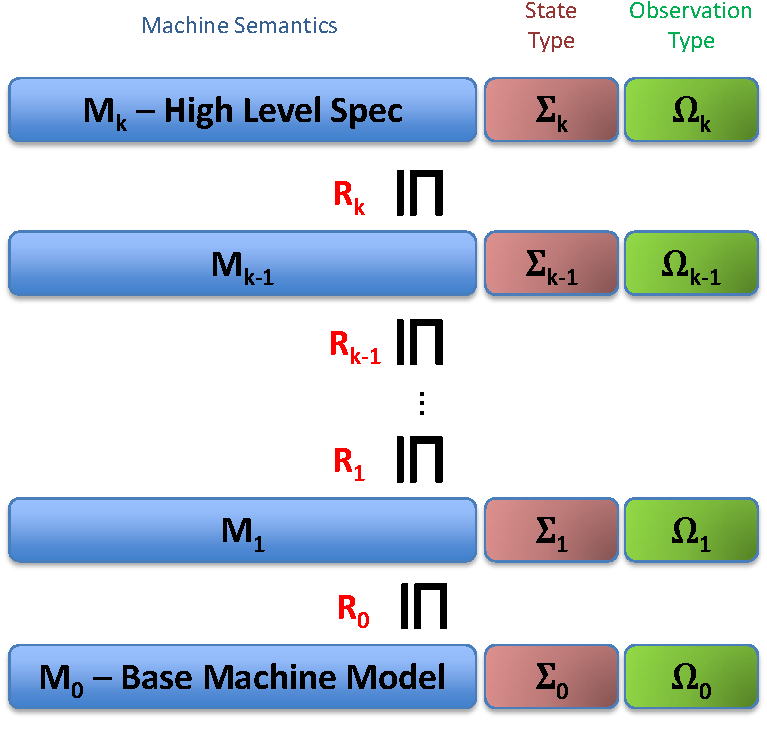
\includegraphics[scale=0.53]{pldi/figure/simulations.pdf}}
\caption{\small{Basic Setup~--- Many simulations are chained together to 
incrementally refine a top-level specification semantics into a
concrete implementation executing over a low-level assembly machine
model.}}
%\vspace*{-2ex}
\label{simulations}
\end{figure}

\section{Machines with Observations}
\label{methodology-machine}

In the following, assume we have a set $\mathcal{P}$ of distinct 
principals or security domains.

\begin{definition}[Machine]
A \emph{state transition machine} $M$ consists 
of the following components (assume all sets may be finite or infinite):
\newpage
\begin{itemize} \itemsep 0pt
\item a type $\Sigma_M$ of program state
\item a set of initial states $I_M$ and final states $F_M$
\item a transition (step) relation $T_M$ of type 
$\pwrset{\Sigma_M \times \Sigma_M}$
\item a type $\Omega_M$ of observations
\item an observation function $\observem{M}{p}{\sigma}$ 
of type $\mathcal{P} \times \Sigma_M \to \Omega_M$
\end{itemize}
\end{definition}

\noindent
When the machine $M$ is clear from context, 
we use the notation $\sigma \steprel \sigma'$ to mean
$(\sigma,\sigma') \in T_M$.
For multiple steps, we define $\sigma \steprel^n \sigma'$ in
the obvious way, meaning that there exists a chain of states
$\sigma_0,...,\sigma_n$ with $\sigma = \sigma_0$, $\sigma' = \sigma_n$,
and $\sigma_i \steprel \sigma_{i+1}$ for all $i \in [0,n)$.
We then define $\sigma \steprel^* \sigma'$ to mean that there exists 
some $n$ such that $\sigma \steprel^n \sigma'$, and
$\sigma \steprel^+ \sigma'$ to mean the same but with a nonzero $n$.

Notice that our definition is a bit different from many traditional
definitions of automata, in that we do not define any explicit notion of 
actions on transitions. In traditional definitions, actions are used
to represent some combination of input events, output events, and
instructions/commands to be executed. In our approach, we advocate moving 
all of these concepts into the program state (which can contain both
concrete and logical state)~--- this simplifies the theory,
proofs, and policy specifications.

\paragraph{Initial States vs Initialized States}
Throughout our formalization, we do not require anything regarding 
initial states of a machine. The reason is related to
how we will actually carry out security and simulation proofs in 
practice (described with respect to the mCertiKOS security proof in
Chapters~\ref{casestudy-def-chapter} and~\ref{casestudy-proof-chapter}). We never 
attempt to reason about the true initial state of a machine; instead,
we assume that some appropriate setup/configuration process brings us from
the true initial state to some properly \emph{initialized} state,
and then we perform all reasoning under the assumption of
proper initialization.

\section{High-Level Security}
\label{methodology-security}
As described in Chapter~\ref{informal-chapter}, we use different notions of
security for the high level and the low level. High-level security says
that each individual step preserves indistinguishability. It also
requires a safety proof as a precondition, guaranteeing that 
the machine preserves some initialization invariant $I$.

\begin{definition}[Safety]
We say that a machine $M$ is safe under state predicate $I$, 
written $\safe{M}{I}$, when the following progress and
preservation properties hold:
{\small\begin{align*}
& 1.) \quad \forall \sigma \in I - F_M \such
\exists \sigma' \such \sigma \steprel \sigma' \\
& 2.) \quad \forall \sigma, \sigma' \such
\sigma \in I \land
\sigma \steprel \sigma' \Longrightarrow \sigma' \in I
\end{align*}}
\end{definition}

\begin{definition}[High-Level Security]
\label{high-level-security}
Machine $M$ is secure for principal $p$ under invariant $I$,
written $\secure{M}{I}{l}$, just when:
\begin{align*}
& 1.) \quad \safe{M}{I} \\
& 2.) \quad \forall \sigma_1, \sigma_2 \in I, \,\, \sigma_1', \sigma_2' \such \\
& \qquad \quad 
\observe{p}{\sigma_1} = \observe{p}{\sigma_2} \land 
\sigma_1 \steprel \sigma_1' \land \sigma_2 \steprel \sigma_2' 
\Longrightarrow \observe{p}{\sigma_1'} = \observe{p}{\sigma_2'} \\
& 3.) \quad \forall \sigma_1, \sigma_2 \in I \such \\
& \qquad \quad \Scale[0.95]{\observe{p}{\sigma_1} = \observe{p}{\sigma_2} 
\Longrightarrow (\sigma_1 \in F_M \iff \sigma_2 \in F_M)}
\end{align*}
\end{definition}

\cut{
\noindent
The first property of this definition requires that we have already
established safety before considering security.
The second property is the unwinding condition restricted to
initialization invariant $I$. The third property says that the finality of a state 
is observable to $p$ (again under invariant $I$); it is needed to 
close a potential termination-related security leak.}

\section{Low-Level Security}
For low-level security, as discussed in Section~\ref{informal-methodology}, 
we first must define whole-execution behaviors
with respect to a monotonic observation function.

\begin{definition}[Behavioral State]
\label{behavioral-state}
Given a machine $M$ and a partial order $\preceq$ over the observation 
type $\Omega_M$, we say that a program state $\sigma$ is behavioral
for principal $p$, written $\behaviorals{M}{p}{\sigma}$,
if all executions starting from $\sigma$ respect 
the partial order; i.e., the following monotonicity property holds:
\[\quad \forall \sigma' \such \sigma \steprel^* \sigma' 
\Longrightarrow \observe{p}{\sigma} \preceq \observe{p}{\sigma'}\]
\end{definition}

\begin{definition}[Behavioral Machine]
\label{behavioral-machine}
We say that a machine $M$ is behavioral for principal $p$, written 
$\behavioral{M}{p}$, when the machine has the following components:
\begin{itemize}
\item a partial order $\preceq$ over the observation type $\Omega_M$
\item a proof that all states of $M$ are behavioral for $p$
\end{itemize}
\end{definition}

\noindent
We next give a semiformal definition of whole-execution behaviors. 
The formal Coq definition involves a
combination of inductive and coinductive types (to handle behaviors of
both terminating and non-terminating executions). Note that our 
definition is quite similar to the one used in CompCert~\cite{Leroy-backend},
except that we use state observations as the basic building block, while 
CompCert uses \emph{traces}, which are input/output events labeled on 
transitions.
\begin{definition}[Whole-Execution Behaviors]
Given a machine $M$ with a partial order defined over $\Omega_M$,
and a state $\sigma$ that is behavioral for 
principal $p$, we write $\behavior{M;p}{\sigma}$ to represent the (potentially 
infinite) set of whole-execution behaviors that can arise from some execution 
of $M$ starting from $\sigma$. The behaviors (elements of this set) can 
be one of four kinds: \emph{fault}, \emph{termination}, \emph{silent divergence},
and \emph{reactive divergence}. In the following, variable $o$ ranges over 
observations and $os$ ranges over infinite streams of observations:
\begin{enumerate}
\item $\ttt{Fault}(o) \in \behavior{M;p}{\sigma}$ indicates that there
is an execution $\sigma~\steprel^*~\sigma'$ where $\sigma'$ is not
a final state, $\sigma'$ cannot take a step to any state, and 
$o = \observe{p}{\sigma'}$.
\item $\ttt{Term}(o) \in \behavior{M;p}{\sigma}$ indicates that there
is an execution $\sigma~\steprel^*~\sigma'$ where $\sigma'$ is 
a final state and $o = \observe{p}{\sigma'}$.
\item $\ttt{Silent}(o) \in \behavior{M;p}{\sigma}$ indicates that there
is an execution $\sigma~\steprel^*~\sigma'$ where $o = \observe{p}{\sigma'}$
and there is an infinite execution starting from $\sigma'$ for which all
states in that infinite execution have identical observations (i.e., all
observations are $o$).
\item $\ttt{React}(os) \in \behavior{M;p}{\sigma}$ indicates that there
is an infinite execution starting from $\sigma$ that ``produces'' each of the
infinitely-many observations of $os$ in order. An observation $o$ is ``produced'' 
in an execution when there exists some single step in the execution 
$\sigma'~\steprel~\sigma''$ with $o = \observe{p}{\sigma''}$ and 
$\observe{p}{\sigma'} \neq \observe{p}{\sigma''}$.
\end{enumerate}
\end{definition}

\noindent
We can now define whole-execution security of a behavioral machine as
behavioral equality. Note that, in our final end-to-end security theorem,
the low-level executions in question will be obtained from relating
indistinguishable high-level states across simulation. We hide this
detail for now inside of an abstract indistinguishability relation $\rho$, 
and will revisit the relation later in this section.

\begin{definition}[Low-Level Security]
Given a machine $m$ that is behavioral for principal $p$, we say that $m$ 
is behaviorally secure for $p$ under some indistinguishability relation $\rho$, 
written $\bsecure{m}{\rho}{p}$, just when:
\[\forall \sigma_1, \sigma_2 \such 
\rho(\sigma_1, \sigma_2) \Longrightarrow 
\behavior{m;p}{\sigma_1} = \behavior{m;p}{\sigma_2}\]
\end{definition}

\section{Simulation}
%\label{methodology-simulation}
We next formalize our definition of simulation. It differs
from standard simulations in two primary aspects:
\begin{enumerate}
\item As explained above, we do not require any relationships to 
hold between initial states.
\item As described in Section~\ref{informal-simulation}, we require
simulation relations to preserve state indistinguishability.
\end{enumerate}

\noindent
Recall the indistinguishability preservation property from 
Section~\ref{informal-simulation}:
{\small
\begin{align*}
& \observem{M}{p}{\sigma_1} = \observem{M}{p}{\sigma_2} \land
R(\sigma_1,s_1) \land R(\sigma_2,s_2) \\
& \qquad \Longrightarrow
\observem{m}{p}{s_1} = \observem{m}{p}{s_2}
\end{align*}}%
\noindent{}One option would be to directly add this property
into the definition of a simulation. For reasons that will
become clear later, however, we will actually take a more
roundabout path that defines simulations in such a way that
the above property is \emph{implied} rather than explicitly
required. Whenever we wish to show a simulation from machine $M$
to machine $m$, we require not only a simulation relation $R$
that relates states of $M$ to states $m$, but also a function $f$
that translates observations of $M$ into observations of $m$.
This translation function will be useful later when we need to 
reason about the relationship between simulations and whole-execution
behaviors. A typical example of a translation function can
be seen in the mCertiKOS security proof presented in 
Chapter~\ref{casestudy-def-chapter}: an abstract state observation contains
many various parts including an output buffer, while a concrete state 
observation contains \emph{only} the output buffer; 
hence the function $f$ simply returns the output buffer from the
high-level observation.

\begin{definition}[Simulation]
\label{gensimdef}
Given two machines $M$, $m$, a principal $p$, a relation $R$ between
states of $M$ and states of $m$, and a total function $\obsrel{R}$ from
observations of $M$ to observations of $m$, we say that there is a
simulation from $M$ to $m$ using $R$ and $\obsrel{R}$,
written $\simu{M}{m}{R;\obsrel{R};p}$, when:
{\small
\begin{align*}
& 1.) \quad \forall \sigma, \sigma' \in \Sigma_M, \,\, s \in \Sigma_m \such \\
& \qquad \quad \sigma \steprel \sigma' \land R(\sigma,s) 
\quad \Longrightarrow \quad
\exists s' \in \Sigma_m \such s \steprel^* s' \land R(\sigma',s') \\
& 2.) \quad \forall \sigma \in \Sigma_M, \,\, s \in \Sigma_m \such \\
& \qquad \quad \sigma \in F_M \land R(\sigma,s) \quad \Longrightarrow \quad s \in F_m \\
& 3.) \quad \forall \sigma \in \Sigma_M, \,\, s \in \Sigma_m \such \\
& \qquad \qquad R(\sigma,s) \quad \Longrightarrow \quad 
\obsrel{R}(\observem{M}{p}{\sigma}) = \observem{m}{p}{s}
\end{align*}}
\end{definition}

\noindent
The first property is the main simulation, the second relates final
states, and the third connects $R$ with $\obsrel{R}$ in such a way
that the indistinguishability preservation property from above is
automatically implied.
For presentation purposes, we omit details 
regarding the well-known ``infinite stuttering'' problem 
for simulations
(described, for example, in~\cite{Leroy-backend}). Our Coq
definition of simulation includes a well-founded order that
prevents infinite stuttering.

Notice that, contrary to our discussion earlier, we do not 
define simulations to be relative to an initialization invariant. It would be
completely reasonable to require safety of the higher-level machine
under some invariant, but this actually ends up being redundant.
Since $R$ is an arbitrary relation, we can simply embed an
invariant requirement within $R$. In other words, one should think 
of $R(\sigma,s)$ as saying not only that $\sigma$ and $s$ are related, 
but also that $\sigma$ satisfies an appropriate invariant.

\section{End-to-End Security}
%\label{methodology-end-to-end}

We will now describe the main theorem of our framework: end-to-end 
security. There are too many technical details to present the
entire proof here; instead, we will only state the primary lemmas 
involved, and then prove how these lemmas imply the main theorem.
We begin with two helpful definitions.

\begin{definition}[Bisimulation]
\label{bisimdef}
Given two machines $M$, $m$, a principal $p$, a relation $R$ between
states of $M$ and states of $m$, and an \emph{invertible} function 
$\obsrel{R}$ from observations of $M$ to observations of $m$, 
we say that there is a bisimulation from $M$ to $m$ using $R$ and 
$\obsrel{R}$, written $\bisimu{M}{m}{R;\obsrel{R};p}$, when
$\simu{M}{m}{R;\obsrel{R};p}$ and $\simu{m}{M}{R^{-1};\obsrel{R}^{-1};p}$.
\end{definition}

\begin{definition}[Invariant-Aware Indistinguishability]
{\small
\begin{align*}
& \Theta^{I}_p(\sigma_1,\sigma_2) \isdef 
\sigma_1 \in I \land \sigma_2 \in I \land
\observe{p}{\sigma_1} = \observe{p}{\sigma_2}
\end{align*}}
\end{definition}

\noindent
The following lemma turns a proof of high-level security
into a bisimulation.

\begin{lem}[High-Level Security Bisimulation]
\label{secure-bisim}
{\small
\begin{align*}
& \forall M, I, p \such \secure{M}{I}{p} \Longrightarrow 
\bisimu{M}{M}{\Theta^{I}_p;\mathid;p}
\end{align*}}
\end{lem}

\noindent
The next two lemmas say, respectively, that executions must 
exhibit at least one behavior, and that deterministic executions
exhibit exactly one behavior.

\begin{definition}[Determinism]
We say that a machine $M$ is deterministic, written $\determ{M}$,
when the following properties hold:
{\small
\begin{align*}
& 1.) \quad \forall \sigma, \sigma', \sigma'' \such
\sigma \steprel \sigma' \land \sigma \steprel \sigma''
\Longrightarrow \sigma' = \sigma'' \\
& 2.) \quad \forall \sigma \in F_M \such
\lnot \, \exists \sigma' \such \sigma \steprel \sigma'
\end{align*}}
\end{definition}

\begin{lem}[Behavior Exists]
\label{beh-exists}
{\small
\begin{align*}
& \forall M, p, \sigma \such \behaviorals{M}{p}{\sigma}
\Longrightarrow
\behavior{M;p}{\sigma} \neq \emptyset
\end{align*}}
\end{lem}

\begin{lem}[Behavior Determinism]
\label{beh-det}
{\small
\begin{align*}
& \forall M, p, \sigma \such 
\behaviorals{M}{p}{\sigma} \land \determ{M} \Longrightarrow
| \behavior{M;p}{\sigma} | = 1
\end{align*}}
\end{lem}

\begin{comment}
\begin{lem}[Behavior Safety]
\begin{align*}
& \forall M, I, l, \sigma \such \\
& \qquad \behaviorals{M}{l}{\sigma} \land \safe{M}{I} \land \sigma \in I \\
& \qquad \Longrightarrow 
\forall o \such \ttt{Fault}(o) \notin \behavior{M;l}{\sigma}
\end{align*}
\end{lem}
\end{comment}

\noindent
The remaining lemmas convert simulations and bisimulations
into behavior subset and equality, respectively. There is one significant 
barrier to stating these lemmas, however:
behaviors are defined in terms of observations, and the types of 
observations of two different machines may be different. Hence
we technically cannot compare behavior sets directly using standard 
subset or set equality, as the types may not match.
To solve this problem, we will exploit our observation translation 
function. This is, in fact,
the reason we use a translation function to define simulations
instead of directly using the indistinguishability preservation 
property. 

In the following, we overload $\obsrel{R}$ to apply
to individual behaviors in the obvious way 
(e.g., $\obsrel{R}(\ttt{Term}(o)) = \ttt{Term}(\obsrel{R}(o))$).
Given a simulation $\simu{M}{m}{R;\obsrel{R};p}$, with both $M$ and
$m$ behavioral for $p$, we define the subset relation
between sets of behaviors by applying $\obsrel{R}$ to every element 
of the first set:
\begin{definition}[Behavior Subset]
\label{beh-subset}
{\small
\begin{align*}
& \simu{\behavior{M;p}{\sigma}}{\behavior{m;p}{s}}{\obsrel{R}}
\isdef \\
& \qquad \forall b \such b \in \behavior{M;p}{\sigma} \Longrightarrow
\obsrel{R}(b) \in \behavior{m;p}{s}
\end{align*}}
\end{definition}

\noindent
Similarly, for \emph{invertible} $\obsrel{R}$, we can define equality
of behavior sets:

\begin{definition}[Behavior Set Equality]
\label{beh-equality}
{\small
\begin{align*}
& \bisimu{\behavior{M;p}{\sigma}}{\behavior{m;p}{s}}{\obsrel{R}}
\isdef \\
& \qquad \simu{\behavior{M;p}{\sigma}}{\behavior{m;p}{s}}{\obsrel{R}}
\land \simu{\behavior{m;p}{s}}{\behavior{M;p}{\sigma}}{\obsrel{R}^{-1}}
\end{align*}}
\end{definition}

\noindent
We now have the machinery to state the two remaining
lemmas:

\begin{lem}[Simulation and Safety Imply Behavior Subset]
\label{beh-sim-subset}
{\small
\begin{align*}
& \forall M, m, I, R, 
\obsrel{R},
p, \sigma, s \such \\
& \qquad
\behaviorals{M}{p}{\sigma} \land \behaviorals{m}{p}{s} 
\land \safe{M}{I} \land 
\simu{M}{m}{R;\obsrel{R};p}
\land \sigma \in I \land R(\sigma,s) \\
& \qquad \Longrightarrow 
\simu{\behavior{M;p}{\sigma}}{\behavior{m;p}{s}}{\obsrel{R}}
\end{align*}}
\end{lem}

\begin{lem}[Bisimulation Implies Behavior Equality]
\label{beh-bisim}
{\small
\begin{align*}
& \forall M, m, R, 
\obsrel{R},
p, \sigma, s \such \\
& \qquad
\behaviorals{M}{p}{\sigma} \land \behaviorals{m}{p}{s} 
\land 
\bisimu{M}{m}{R;\obsrel{R};p} \land R(\sigma,s) \\
& \qquad \Longrightarrow 
\bisimu{\behavior{M;p}{\sigma}}{\behavior{m;p}{s}}{\obsrel{R}}
\end{align*}}
\end{lem}

\paragraph{Technical Aside}
These two lemmas are not quite true as stated. If
a single step in machine $M$ produces an event (i.e., changes
the state observation) and is simulated by multiple steps in
$m$, it could be the case that those multiple steps produce
multiple events. In our Coq proof, we resolve this problem by
defining a notion of ``measure'' that maps observations to
natural numbers, and by requiring that (1) single steps never increase
measure by more than one; and that (2) the observation translation function
preserves measure.
For example, the measure of an output buffer is defined to be its size,
and no single step is allowed to append more than one output to the buffer.
This is sufficient for conducting our mCertiKOS proof, but it is unfortunately a 
rather ad-hoc solution; we hope that future work will yield a cleaner one.

\vspace{0.5in}
We have now stated all the required lemmas, and can move on
to our primary theorem guaranteeing that simulations preserve
security. As mentioned previously, 
low-level security uses an indistinguishability relation derived
from high-level indistinguishability and a simulation relation:
\begin{definition}[Low-Level Indistinguishability]
\label{ll-rho}
{\small\begin{align*}
& \phi(M,p,I,R) \isdef \\
& \quad \lambda s_1, s_2 \such 
\exists \sigma_1, \sigma_2 \in I \such 
\observem{M}{p}{\sigma_1} = \observem{M}{p}{\sigma_2} 
\land R(\sigma_1,s_1) \land R(\sigma_2,s_2)
\end{align*}}
\end{definition}

\noindent
\begin{thm}[End-to-End Security]
\label{end-to-end}
Suppose we have two machines $M$ and $m$, a principal $p$, a
high-level initialization invariant $I$, and 
a simulation $\simu{M}{m}{R;f;p}$. Further suppose that
$m$ is deterministic and behavioral for $p$.
Let low-level indistinguishability relation $\rho$ be 
$\phi(M,p,I,R)$ from Definition~\ref{ll-rho}. Then high-level security
implies low-level security:
\[\secure{M}{I}{p} \Longrightarrow \bsecure{m}{\rho}{p}\]
\end{thm}

\begin{proof}
For the first part of the proof, we define a new machine $N$ in between $M$
and $m$, and prove simulations from $M$ to $N$ and from $N$
to $m$. $N$ will mimic $M$ in terms of program states
and transitions, while it will mimic $m$ in terms of observations.
More formally, we define $N$ to have the following components:
\begin{itemize}
\item program state $\Sigma_M$
\item initial states $I_M$
\item final states $F_M$
\item transition relation $T_M$
\item observation type $\Omega_m$
\item observation function 
$\observem{N}{p}{\sigma} \isdef \obsrel{R}(\observem{M}{p}{\sigma})$
\end{itemize}

First, we establish the simulation $\simu{M}{N}{\mathid;\obsrel{R};p}$.
Referring to Definition~\ref{gensimdef}, the first two properties hold
trivially since $N$ has the same transition relation and final
state set as $M$. The third property reduces to exactly our
definition of $\observem{N}{p}{-}$ given above.

Next, we establish the simulation $\simu{N}{m}{R;\mathid;p}$. The
first two properties of Definition~\ref{gensimdef} are exactly
the same as the first two properties of the provided simulation
$\simu{M}{m}{R;\obsrel{R};p}$, and thus they hold. For the third
property, assuming we know $R(\sigma,s)$, we have 
$\mathid(\observem{N}{p}{\sigma}) = 
\observem{N}{p}{\sigma} = \obsrel{R}(\observem{M}{p}{\sigma})
= \observem{m}{p}{s}$, where the final equality comes from
the third property of the provided simulation.

For the next part of the proof, we unfold the definition of
what we are trying to prove, $\bsecure{m}{\phi(M,p,I,R)}{p}$. This
yields: 
\begin{align*}
& \forall s_1, s_2 \such 
(\exists \sigma_1, \sigma_2 \in I \such 
\observem{M}{p}{\sigma_1} = \observem{M}{p}{\sigma_2}
\land R(\sigma_1,s_1) \land R(\sigma_2,s_2)) \\
& \qquad \Longrightarrow 
\behavior{m;p}{s_1} = \behavior{m;p}{s_2}
\end{align*}%

\noindent{}Pick any states $s_1$, $s_2$, $\sigma_1$, $\sigma_2$ such 
that $\sigma_1 \in I$, $\sigma_2 \in I$, 
$\observem{M}{p}{\sigma_1} = \observem{M}{p}{\sigma_2}$,
$R(\sigma_1,s_1)$, and $R(\sigma_2,s_2)$. We will prove the
desired $\behavior{m;p}{s_1} = \behavior{m;p}{s_2}$
by relating the behaviors of $N$ with those of $m$. 
In order to do this, however, we first must show that $N$ has 
well-defined behaviors for executions starting from $\sigma_1$
or $\sigma_2$. In other words, we must prove 
$\behaviorals{N}{p}{\sigma_1}$ and $\behaviorals{N}{p}{\sigma_2}$.
We will focus on the proof for $\sigma_1$; the other proof is
analogous. We use the same partial order as provided
by the assumption $\behavioral{m}{p}$.
Consider any execution $\sigma_1~\steprel^*~\sigma_1'$ in $N$.
Since $R(\sigma_1,s_1)$, we can use the simulation 
$\simu{N}{m}{R;\mathid;p}$ established above, yielding an execution
$s_1~\steprel^*~s_1'$, for some $s_1'$ (technically, the simulation 
property only applies to single steps in the higher machine; 
however, it can easily be extended to multiple steps
through induction on the step relation). Additionally, we have 
$R(\sigma_1,s_1)$ and $R(\sigma_1',s_1')$, implying by the third property 
of simulation that $\observem{N}{p}{\sigma_1} = \observem{m}{p}{s_1}$ and 
$\observem{N}{p}{\sigma_1'} = \observem{m}{p}{s_1'}$.
Since $m$ is behavioral, we also have 
$\observem{m}{p}{s_1}~\preceq~\observem{m}{p}{s_1'}$. Hence we conclude
$\observem{N}{p}{\sigma_1}~\preceq~\observem{N}{p}{\sigma_1'}$, as desired.

We now know that $\behaviorals{N}{p}{\sigma_1}$ and 
$\behaviorals{N}{p}{\sigma_2}$. Notice that
when $\obsrel{R}$ is $\mathid$, our definitions of behavior subset and
equality (Definitions~\ref{beh-subset} and~\ref{beh-equality}) reduce
to standard subset and set equality. Therefore, applying 
Lemma~\ref{beh-sim-subset} to the established simulation
$\simu{N}{m}{R;\mathid;p}$ tells us that 
$\behavior{N;p}{\sigma_1}~\subseteq~\behavior{m;p}{s_1}$
and $\behavior{N;p}{\sigma_2}~\subseteq~\behavior{m;p}{s_2}$ (note that
the safety precondition of Lemma~\ref{beh-sim-subset} holds because $M$ and $N$
have the same state type and transition relation, and high-level security 
of $M$ implies safety). Furthermore,
since $m$ is deterministic, Lemma~\ref{beh-det} gives us 
$| \behavior{m;p}{s_1} | = | \behavior{m;p}{s_2} | = 1$. Since 
Lemma~\ref{beh-exists} guarantees that neither $\behavior{N;p}{\sigma_1}$ nor
$\behavior{N;p}{\sigma_2}$ is empty, we conclude that
$\behavior{N;p}{\sigma_1} = \behavior{m;p}{s_1}$
and $\behavior{N;p}{\sigma_2} = \behavior{m;p}{s_2}$.

To complete the proof, we now just need to show that 
$\behavior{N;p}{\sigma_1} = \behavior{N;p}{\sigma_2}$. Applying
Lemma~\ref{secure-bisim} to our assumption of high-level security of $M$
gives us the bisimulation $\bisimu{M}{M}{\Theta^{I}_p;\mathid;p}$.
We would like to apply Lemma~\ref{beh-bisim}, but we first need
to convert this bisimulation into one on $N$, since $M$ is not
behavioral. Since $M$ and $N$ share program state type, final states,
and transition relation, it is not difficult to see that the first
two required properties of the simulation $\simu{N}{N}{\Theta^{I}_p;\mathid;p}$ 
hold. If we can establish the third property, then we will obtain the
desired bisimulation $\bisimu{N}{N}{\Theta^{I}_p;\mathid;p}$ since $\mathid$ 
is obviously invertible and $\Theta^{I}_p$ is symmetric. The third
property requires us to prove that 
$\Theta^{I}_p(\sigma_1,\sigma_2) \Longrightarrow 
\observem{N}{p}{\sigma_1} = \observem{N}{p}{\sigma_2}$.
By definition, $\Theta^{I}_p(\sigma_1,\sigma_2)$ implies that
$\observem{M}{p}{\sigma_1} = \observem{M}{p}{\sigma_2}$.
Notice that $\observem{N}{p}{\sigma_1} = \observem{N}{p}{\sigma_2}$
following from this fact is exactly the indistinguishability 
preservation property we discussed earlier. Indeed, we
have $\observem{N}{p}{\sigma_1} = \obsrel{R}(\observem{M}{p}{\sigma_1}) = 
\obsrel{R}(\observem{M}{p}{\sigma_2}) = \observem{N}{p}{\sigma_2}$.

Finally, we instantiate Lemma~\ref{beh-bisim} with both machines
being $N$. Notice that the required
precondition $\Theta^{I}_p(\sigma_1,\sigma_2)$ holds by assumption.
Lemma~\ref{beh-bisim} now gives us the conclusion
$\bisimu{\behavior{N;p}{\sigma_1}}{\behavior{N;p}{\sigma_2}}{\mathid}$.
As mentioned earlier, behavior equality reduces to standard set
equality when $\obsrel{R}$ is $\mathid$, and so we get the desired
$\behavior{N;p}{\sigma_1} = \behavior{N;p}{\sigma_2}$. 
\end{proof}






\chapter{Security Overview of mCertiKOS}
\label{casestudy-def-chapter}
%\section{Security Definition of mCertiKOS}
%\label{casestudy-def}

We will now discuss how to apply the methodology of
Chapters~\ref{informal-chapter} and~\ref{methodology-chapter} to
formally guarantee end-to-end isolation between user 
processes running on top of the mCertiKOS kernel~\cite{certikos-popl}. 
During the proof effort, we had to make some changes to the operating
system to close potential security holes. We refer to our secure 
variant of the kernel as mCertiKOS-secure.

\section{mCertiKOS Overview}

The starting point for our proof effort was the basic version of
the mCertiKOS kernel, described in detail in Section~7 
of~\cite{certikos-popl}. We will give an overview of the kernel
here. It is composed of $32$ abstraction \emph{layers},
which incrementally build up the concepts of physical memory
management, virtual memory management, kernel-level processes,
and user-level processes. Each layer $L$ consists of the
following components:
\begin{itemize}
\item a type $\Sigma_L$ of program state, separated into 
machine registers, concrete memory, and abstract data of type $D_L$
\item a set of initial states $I_L$ and final states $F_L$
\item a set of primitives $P_L$ implemented by the layer
\item for each $f \in P_L$, a deterministic specification of type
$\Sigma_L \to \option{\Sigma_L}$
\item \textit{(if $L$ is not the bottom layer)} for each  
$f \in P_L$, an implementation written
in either LAsm$(L')$ or ClightX$(L')$ (defined below), where 
$L'$ is the layer below $L$
\item two special primitives called \ttt{load} and \ttt{store}
that model access to global memory; these primitives have no 
implementation as they are a direct model of how the x86 machine
translates virtual addresses using page tables
\end{itemize}

The top layer is called TSysCall, and the bottom is called
MBoot. MBoot describes execution over the model of the actual hardware;
the specifications of its primitives are taken as axioms. Implementations
of primitives in all layers are written in either a layer-parameterized
variant of x86 assembly or a layer-parameterized variant of C. 

The assembly language, called LAsm$(L)$, is an extension of 
CompCert's~\cite{compcert} model of x86 assembly that allows primitives
of layer $L$ to be called atomically. When an atomic primitive call
occurs, the semantics consults that primitive's specification
to take a step. Note that the \ttt{load} and \ttt{store} primitives are never
called explicitly (as they have no implementation), but instead
are used to specify the semantics of x86 instructions that read or
write memory (e.g., \ttt{movl \%eax, 0(\%ecx)}).

The C variant, called ClightX$(L)$, is an extension of
CompCert's Clight language~\cite{blazy-leroy-clight} (which is a 
slightly-simplified version of C). Like LAsm$(L)$, the semantics
is extended with the ability to call the primitives of $L$
atomically. ClightX$(L)$ programs can be compiled to LAsm$(L)$
in a verified-correct fashion using the CompCertX 
compiler~\cite{certikos-popl}, which is an extension of 
CompCert\ifextended~that supports per-function compilation\else\fi.

Each layer $L$ induces a machine $M_L$ of the kind described in
Section~\ref{methodology-machine}\ifextended. The state type and initial/final states
of $M_L$ come directly from $L$. The transition relation of
type $\pwrset{\Sigma_L \times \Sigma_L}$ is precisely the operational 
semantics of LAsm$(L)$. The machine's observation function will be 
discussed later, as it is an extension that we implemented over
the existing mCertiKOS specifically for the security proof.
\else, with transition relation defined
by the operational semantics of LAsm$(L)$.
\fi

\begin{comment}
\paragraph{Load/Store Primitives}
Before continuing, there is one somewhat technical detail 
regarding the LAsm$(L)$ semantics that requires explanation. 
While most layer primitives are called in LAsm$(L)$ using 
the \ttt{call} syntax, the special \ttt{load} and \ttt{store}
primitives work differently. Whenever an
assembly command dereferences an address, the LAsm$(L)$
semantics consults the load/store primitives to decide 
how the dereference is actually resolved. 
As an example, consider the following snippet
of assembly code, taken from the implementation of the
page fault handler TSysCall primitive:
{\small
\begin{alltt}
   call trap_get
   movl \%eax, 0(\%esp)   
   call ptfault_resv
\end{alltt}
}
\noindent
The layer below TSysCall is called TDispatch, and thus this
code is written in the language LAsm(TDispatch).
The first and third lines call primitives of TDispatch
atomically. The second line ostensibly writes the value 
of EAX into the memory location pointed to by ESP. The 
actual semantics of this line, however, will call
TDispatch's \ttt{store} primitive with the value of EAX and the
address in ESP as parameters. This primitive will
translate the destination address from virtual to physical
by walking through the page tables of the currently-executing
process.
\end{comment}

\begin{figure}
\centering{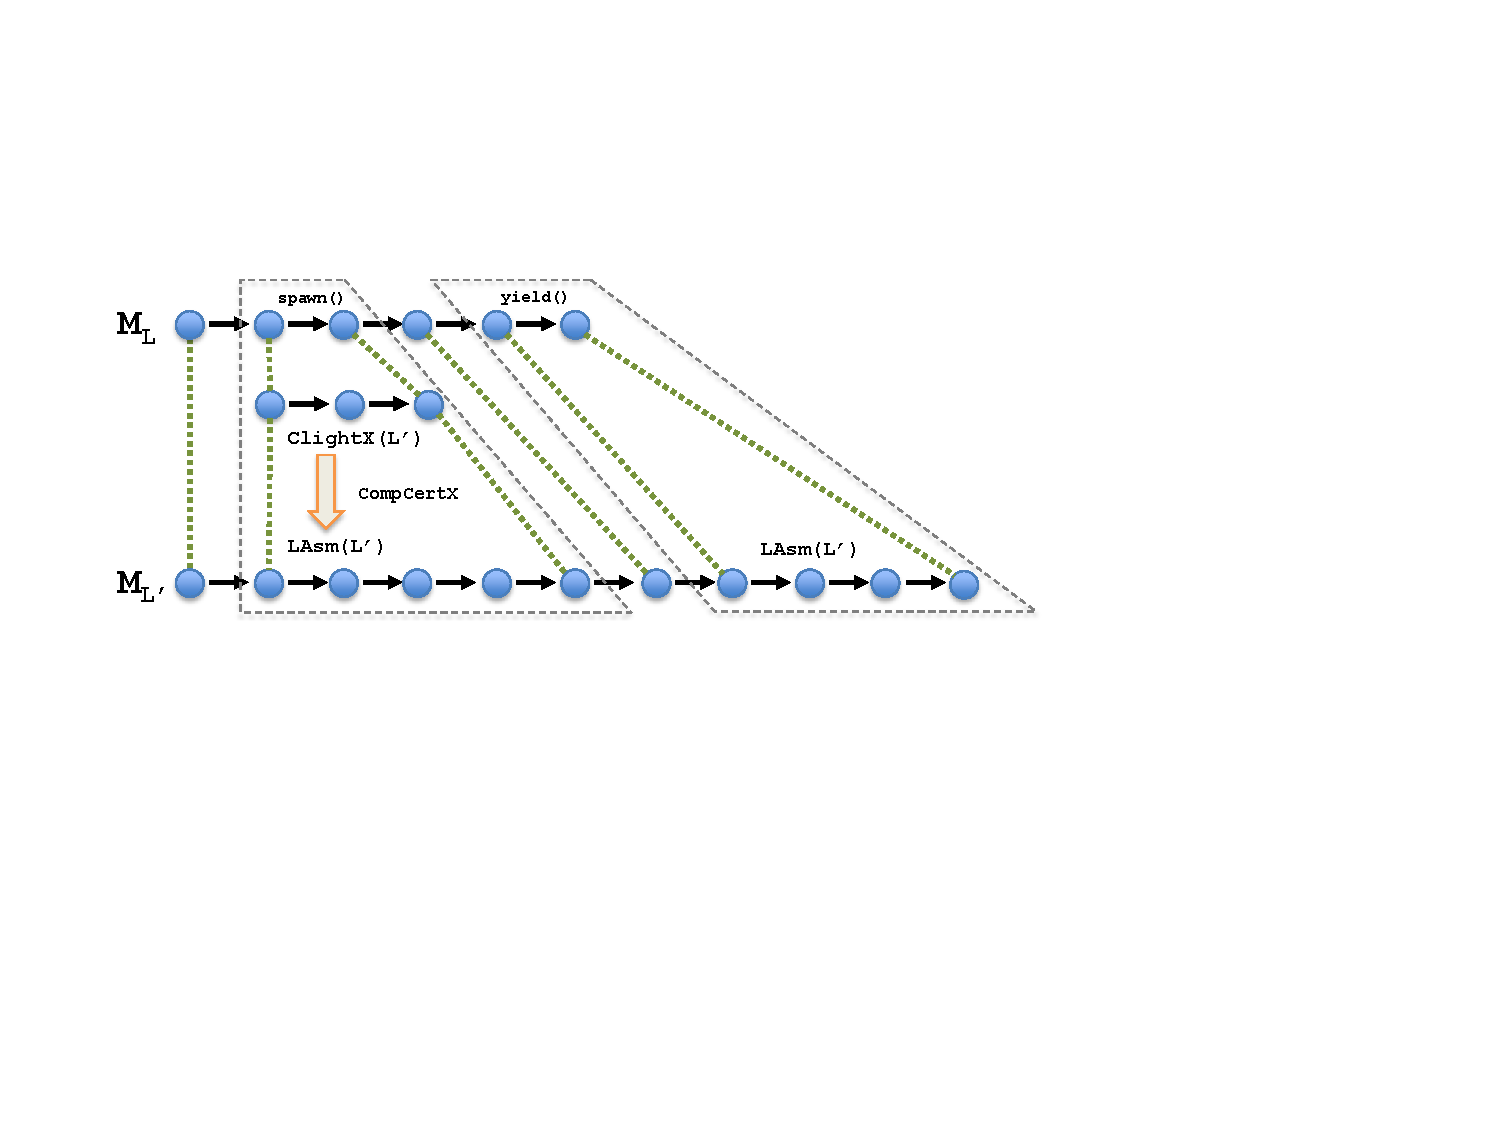
\includegraphics[scale=0.53]{pldi/figure/layer-sim.pdf}}
\caption{\small{Simulation between adjacent layers.
Layer $L$ contains primitives \ttt{spawn} and \ttt{yield},
with the former implemented in ClightX$(L')$ and the latter
implemented in LAsm$(L')$.}}
%\vspace*{-2ex}
\label{layer-sim}
\end{figure}

\paragraph{Layer Simulation}
Figure~\ref{layer-sim} illustrates how machines induced by two 
consecutive layers are connected via simulation. Each step 
of machine $M_L$ is either a standard assembly command
or an atomic primitive call. Steps of the former category are
simulated in $M_{L'}$ by exactly the same assembly command.
Steps of the latter are simulated using the primitive's 
implementation, supplied by layer $L$. If the primitive is
implemented directly in LAsm$(L')$ (e.g., \ttt{yield} in Figure~\ref{layer-sim}), 
then the simulation directly 
uses the small-step semantics of this implementation. If the primitive is
implemented in ClightX$(L')$ (e.g., \ttt{spawn} in Figure~\ref{layer-sim}), 
then CompCertX's compilation is inserted into the simulation. CompCertX is
verified to provide a simulation from the ClightX$(L')$
execution to the corresponding LAsm$(L')$ execution, so 
this is chained appropriately to get an end-to-end
simulation from the $M_L$ execution to the $M_{L'}$
execution.

As a general convention, the simulation relation between 
consecutive machines only represents an abstraction of
some concrete memory into abstract data. In other words,
some portion of concrete memory in the lower-level machine is related
to some newly-introduced portion of abstract data in the higher-level 
machine. In this way, as we move up the layers, concrete memory gets
incrementally abstracted away in a monotonic fashion.
Once we reach the top layer, TSysCall, 
concrete memory has been fully abstracted away from user-mode
semantics; hence user processes have no mechanism for interacting
with the concrete memory directly. In fact, by convention, 
mCertiKOS actually requires that primitive specifications
at \emph{all} layers do not interact with concrete memory.
If a primitive needs to access some portion of concrete memory,
then a layer must first be introduced to abstract that memory.

Once every pair of consecutive machines is connected with a
simulation, they are combined transitively to 
obtain a simulation from TSysCall to MBoot. Since the TSysCall layer
provides mCertiKOS's system calls as primitives, user process
execution is specified at the TSysCall level.
To get a better sense of user process execution, we will now 
describe the abstract data and primitives of the TSysCall layer 
in mCertiKOS-secure.

\begin{comment}
\begin{figure}
\centering{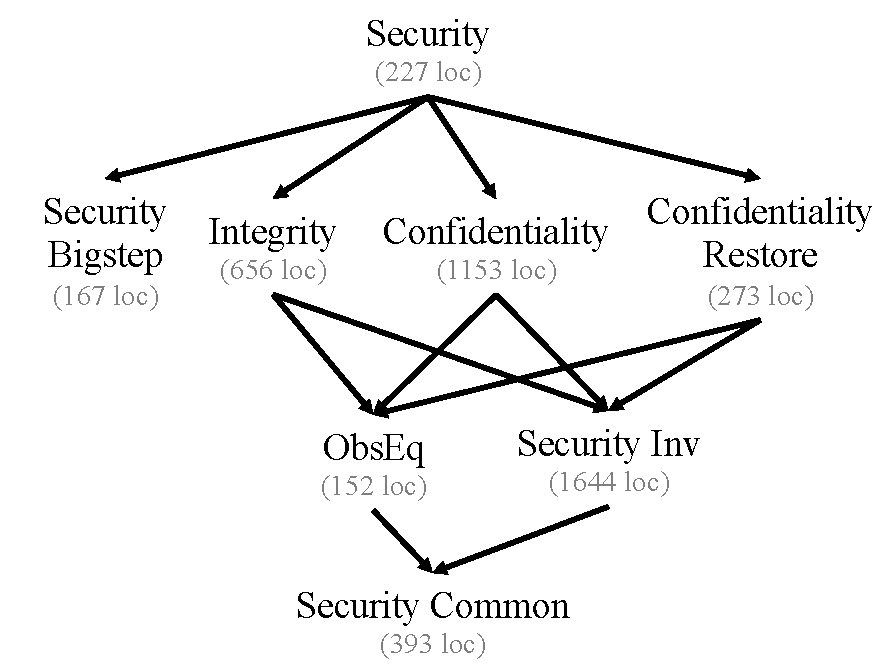
\includegraphics[scale=0.5,origin=c]{figure/code_structure.pdf}}
\caption{\small{Dependencies and line counts of security-related proofs. Note 
that most of the new invariants in SecurityInv were needed for
confidentiality, so the relative effort required for proving
confidentiality is larger than it appears from the line counts.}}
\label{files}
\end{figure}

The entire Coq code base of mCertiKOS-secure can be found in the
supplementary material~\cite{costanzo-popl16-tr}. The security proof
can be found within the \ttt{security} directory. Figure~\ref{files}
names all of the relevant Coq files in the \ttt{security} directory,
and shows their dependency relations and line counts ignoring blank
lines. This figure can be used to maintain a high-level understanding
of the proof structure as we delve into the proof details throughout
this section and the next.
\end{comment}

\paragraph{TSysCall State}
The TSysCall abstract data is a Coq record consisting of $32$
separate fields. We list here those fields that will be
relevant to our discussion later. In the following, whenever a field 
name has a subscript of $i$, the field is a finite map from 
process ID to some data type. Each user process running over the
kernel has a unique, integer-valued process ID, and IDs are never
reused. From a security standpoint, one should think of each process
ID value as a unique principal or security domain.

\begin{itemize}
\item $\ttt{out}_i$~--- The output buffer for process $i$\ifextended,
represented as a list of $32$-bit integers\else\fi.
Note that output buffers
exist in all layers' abstract data, including MBoot. They are
never actually implemented in memory; instead, they are assumed to be
a representation of some external method of output (e.g., a monitor
or a network channel), and are used to define the observable
events of user-process execution.
\ifextended
\item $\ttt{ikern}$~--- A global boolean flag stating whether
the machine is currently in kernel mode or user mode.
\else\fi
\item $\ttt{HP}$~--- A global, flat view of the user-space
memory heap\ifextended~(physical addresses between $2^{30}$ and 
$3 \times 2^{30}$)\else\fi.
A \emph{page} is defined as the $4096$-byte sequence starting 
from a physical address that is divisible by $4096$.
\item $\ttt{AT}$~--- A global allocation table, represented as
a bitmap indicating which pages in the global heap have been 
allocated. Element $n$ corresponds to 
\ifextended
the $4096$-byte page starting from physical address $4096n$.
\else page $n$. 
\fi
\item $\ttt{pgmap}_i$~--- A representation of the two-level page 
map for process $i$. The page map tells the x86 machine how
to translate virtual addresses between $0$ and $2^{32} - 1$ into 
physical addresses.
\item $\ttt{container}_i$~--- Metadata for process $i$
regarding spawned status, children,
parents, and resource quota. A container is itself a 
Coq record containing the following fields:
\begin{itemize}
\item $\ttt{used}$~--- A boolean indicating whether process $i$ has
been spawned.
\item $\ttt{parent}$~--- The ID of the parent of process 
$i$\ifextended~(or $0$ for root process $0$)\else\fi.
\item $\ttt{nchildren}$~--- The number of children of process $i$.
\item $\ttt{quota}$~--- The maximum number of pages that process
$i$ is allowed to allocate.
\item $\ttt{usage}$~--- The current number of pages that process
$i$ has allocated.
\end{itemize}
%There are a number of invariants maintained that guarantee the
%container structure forms a valid tree. Furthermore, a process's
%quota is always at least as large as the sum of its childrens'
%quotas, meaning that the root (process $0$) quota provides an
%upper bound for the whole system.
\item $\ttt{ctxt}_i$~--- The saved register context of 
process $i$, containing the register values that will need to 
be restored the next time process $i$ is scheduled.
\item $\ttt{cid}$~--- The currently-running process ID.
\ifextended
\item $\ttt{rdyQ}$~--- An ordered list of process IDs that are
ready to be scheduled (head of the list is the next to be scheduled).
\else\fi
\end{itemize}

\noindent
Note that process containers, which track parent/child relationships
and dynamic resource usage, did not exist in the initial version of 
mCertiKOS taken from~\cite{certikos-popl}. Prior to conducting
our security proof, we realized that a lack of dynamic resource
tracking would be extremely problematic for security, since a
user process could easily affect others via a denial-of-service
attack that repeatedly allocates pages until all of physical memory
is exhausted. Therefore, inspired by the concept of containers
in the HiStar security-aware operating system~\cite{histar}, we
chose to implement a similar notion of container objects in 
mCertiKOS to preemptively deal with this security issue. Containers
not only enforce a quota on the number of memory pages each process 
is allowed to dynamically allocate, but they also allow processes to
distribute some of their memory quota to children. In 
Chapter~\ref{casestudy-proof-chapter}, we will illustrate  
how containers and memory quotas are crucial to our security proof.

\paragraph{TSysCall Primitives}
There are $9$ primitives in the TSysCall layer of mCertiKOS-secure, including the
load/store primitives. The primitive specifications operate over
both the TSysCall abstract data and the machine registers.
Note that they do not interact with concrete memory since all 
relevant portions of memory have already been abstracted
into the TSysCall abstract data.

\begin{itemize}
\item \emph{Initialization}~--- \ttt{proc\_init} sets up the various kernel 
objects to get everything into a working state. We never attempt to 
reason about anything
that happens prior to initialization; it is assumed that the bootloader
will always call \ttt{proc\_init}.
\item \emph{Load/Store}~--- Since paging is enabled in all user-mode 
TSysCall states, the \ttt{load} and \ttt{store} primitives walk the 
two-level page table of the currently-running process to
translate a virtual address into physical. If no physical address is
found due to no page being mapped, then the faulting virtual address is
written into the CR2 control register, the current register context
is saved, and the instruction pointer register is updated to point to 
the entry of the page fault handler primitive.
\item \emph{Page Fault}~--- \ttt{pgf\_handler} is called immediately after one 
of the load/store primitives fails to resolve a virtual address. It reads
the faulting virtual address from the CR2 register, allocates one or two 
new pages as appropriate, increases the current process's page usage
(see the \ttt{container} description above),
and plugs the page(s) into the page table.
It then restores the register context that was saved when the 
load/store primitive faulted. If the current process does not
have enough available quota to allocate the required pages, then
the instruction pointer register is updated to point to the entry
of the yield primitive (see below). \cut{This means that the process will
end up page faulting and yielding infinitely.}
\item \emph{Get Quota}~--- \ttt{get\_quota} returns the amount of remaining 
quota for the currently-executing process. This is useful to provide
as a system call since it allows processes to divide their
quota among children in any way they wish.
\item \emph{Spawn Process}~--- \ttt{proc\_create} attempts to spawn a new 
child process. It takes a quota as a parameter, specifying the maximum number 
of pages the child process will be allowed to allocate. This quota allowance 
is taken from the current process's available quota.
\item \emph{Yield}~--- \ttt{sys\_yield} performs the first step for 
yielding\cut{ to the next process in the ready queue}. 
It enters kernel mode, disables paging, saves the current registers, and changes
the currently-running process ID to the head of the ready queue (updating
the ready queue accordingly). It then 
context switches by restoring the newly-running process's registers. The 
newly-restored instruction pointer register is guaranteed (proved as an invariant) to 
point to the function entry of the \ttt{start\_user} primitive.
\item \emph{Start User}~--- \ttt{start\_user} performs the simple second step
of yielding. It enables paging for the currently-running process and exits
kernel mode. The entire functionality of yielding must be split into
two primitives (\ttt{sys\_yield} and \ttt{start\_user}) because
context switching requires writing to the instruction pointer register,
and therefore only makes sense when it is the final operation performed by
a primitive. 
Hence yielding is split into one primitive that ends with a 
context switch, and a second primitive that returns to user mode.
\item \emph{Output}~--- \ttt{print} appends its integer parameter to the
output buffer of the currently-running process.
\end{itemize}

\section{Security Overview}
\label{ssec:security-overview}

\cut{We have now provided enough background on mCertiKOS to begin discussing
the security verification.}
We consider each process ID to be a
distinct principal\cut{ or security domain}. 
The security property that we aim to prove is exactly the high-level
security defined in Section~\ref{methodology-security} 
(Definition~\ref{high-level-security}), applied over the TSysCall machine 
using a carefully-constructed observation function that we define below. 
Theorem~\ref{end-to-end} then guarantees security of 
the corresponding whole-execution behaviors over the MBoot machine 
(which represents our lowest-level model of the assembly machine).

\paragraph{High-Level Semantics}
\ifextended
As explained in Chapters~\ref{informal-chapter} and~\ref{methodology-chapter},
high-level
\else
High-level \fi 
security is proved by showing that every step of
execution preserves an indistinguishability relation saying 
that the observable portions of two states are equal. In
the mCertiKOS context, however, this property will not actually
hold over the TSysCall machine, because it models the
execution of \emph{all} user processes, not just the observer's process.

To see this, consider any process ID $p$, which we
call the observer process. For any TSysCall state $\sigma$, we say
that $\sigma$ is ``active'' if \ttt{cid}$(\sigma) = p$, and
``inactive'' otherwise. Now consider whether the values in machine
registers should be observable to $p$. Clearly, if $p$ is executing,
then it can read and write registers however it wishes, so the
registers must be considered observable.  On the other hand, if some
other process $p'$ is executing, then the registers must be
unobservable to $p$ if we hope to prove that $p$ and $p'$ are
isolated. We conclude that registers should be observable to $p$ only
in active states.

What happens, then, if we attempt to prove that 
indistinguishability is preserved when starting from
inactive indistinguishable states? Since the states 
are inactive, the registers are unobservable, and so
the instruction pointer register in particular may have
a completely different value in the two states. This means
that the indistinguishable states may execute different
instructions. If, for example, one state executes the yield primitive
while the other does not, we may end up in a situation
where one resulting state is active but the other is not;
clearly, such states cannot be indistinguishable 
since the registers are observable in one state but not
in the other. Thus indistinguishability will not
be preserved in this example.

The fundamental issue here is that, in order to prove
that $p$ cannot be influenced by $p'$, we must show
that $p$ has no knowledge that $p'$ is even executing
over the kernel. We accomplish this by defining a
higher-level machine above the TSysCall machine, where every state 
is active, meaning the semantics itself hides the executions
of all processes except for the observer. We call this the TSysCall-local 
machine~--- it is parameterized by principal $p$, and it 
represents $p$'s local view of the TSysCall machine.

\begin{figure}
\centering{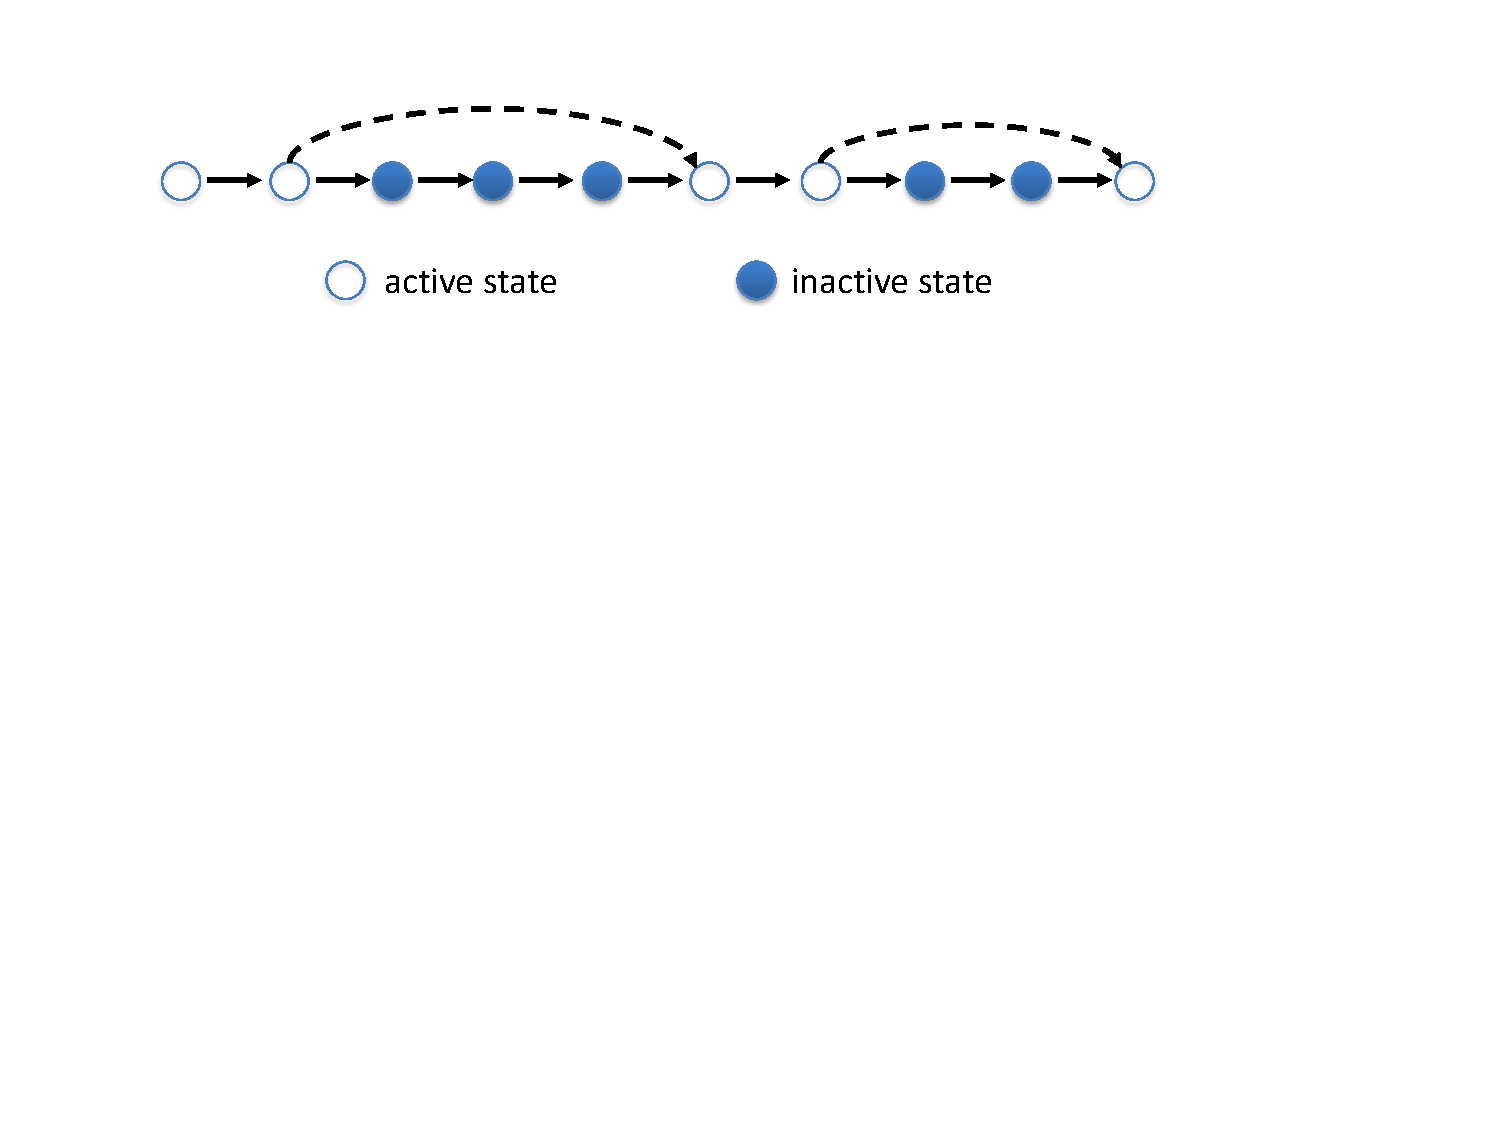
\includegraphics[scale=0.47]{pldi/figure/bigstep.pdf}}
\caption{\small{The TSysCall-local semantics, defined
by taking big steps over the inactive parts of the TSysCall 
semantics.}}
%\vspace*{-2ex}
\label{bigstep}
\end{figure}

Figure~\ref{bigstep} shows how
the semantics of
TSysCall-local is defined. The solid arrows are transitions of
the TSysCall machine, white circles are active TSysCall states, 
and shaded circles are inactive states. The TSysCall-local 
semantics is then obtained by 
combining all of the solid arrows connecting active states
with all of the dotted arrows. Note that in the TSysCall
layer, the yield primitive is the \emph{only} way that
a state can change from active to inactive, or vice-versa.
Thus one can think of the TSysCall-local machine as a
version of the TSysCall machine where the yield semantics
takes a big step over other processes' executions, immediately 
returning to the observer process that invoked the yield.

\ifextended
Given all of this discussion, our
\else Our \fi high-level security
property is proved over the TSys\-Call-local machine, for
\emph{any} choice of observer principal $p$. 
We prove simulation from TSysCall-local to 
TSysCall, so this strategy fits cleanly into our
security verification methodology.

\paragraph{Observation Function}

We now define the high-level observation function used
in our verification\cut{, which maps each principal and state
to an observation}. 
For a given process ID $p$, the state observation
of $\sigma$ is defined as follows:
\begin{itemize} \itemsep 0pt
\item \emph{Registers}~--- All registers are observable
if $\sigma$ is active. \cut{No registers are observable if 
$\sigma$ is inactive.}
\item \emph{Output}~--- The output buffer of $p$ is
observable.
\item \emph{Virtual Address Space}~--- We can dereference 
any virtual address by walking through $p$'s page tables.
This will result in a value if the address is actually
mapped, or no value otherwise. This function from virtual
addresses to option values is observable. Importantly,
the physical address at which a value resides is never
observable.
\item \emph{Spawned}~--- The spawned status of $p$ is observable.
\item \emph{Quota}~--- The remaining quota\cut{ (max quota minus usage)} 
of $p$ is observable.
\item \emph{Children}~--- The number of children
of $p$ is observable.
\item \emph{Active}~--- It is observable whether 
\ttt{cid}$(\sigma)$ is equal to $p$.
\item \emph{Reg Ctxt}~--- The saved register
context of $p$ is observable.
%\item \emph{Page Fault Info}~--- The CR2 register, which
%stores the offending virtual address after a page fault
%occurs, is observable whenever $p$ is active. We will 
%describe this point in some more detail later.
\end{itemize}

%%%%%%%%%%%%%%%%%%%%%%%%%%%%%%%%%%%%%%%%%%%%%%%%%%%%%%%%%%%%%%%%
\begin{figure}[t]
\begin{center}
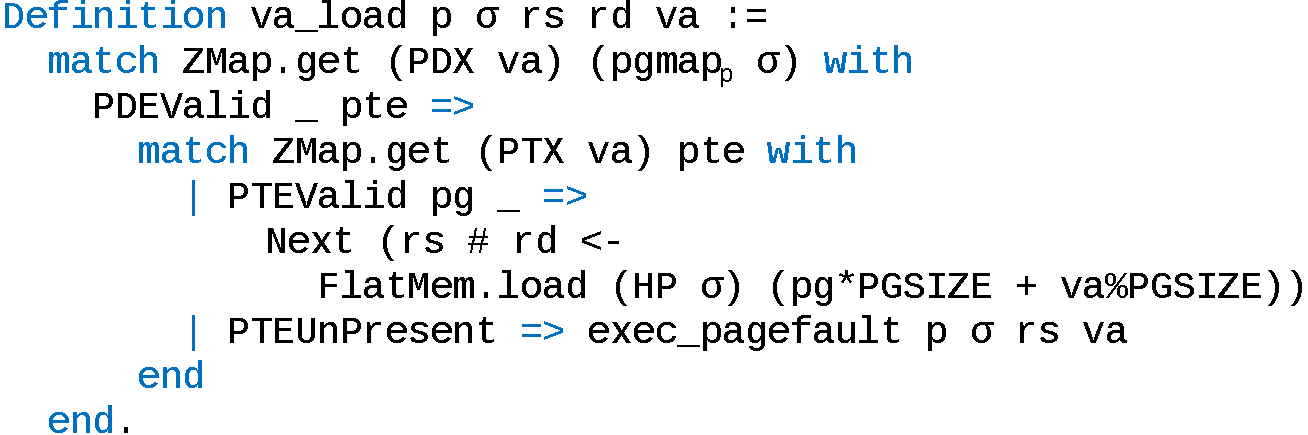
\includegraphics[scale=0.55]{pldi/figure/vaload}
\caption{\small Pseudocode of the \ttt{load} primitive
specification.}
\label{fig:va-load}
%\vspace*{-20pt}
\end{center}
\end{figure}
%%%%%%%%%%%%%%%%%%%%%%%%%%%%%%%%%%%%%%%%%%%%%%%%%%%%%%%%%%%%%%%%

The virtual address space component of the observation 
function is particularly interesting, as it showcases the
strength and generality of our methodology. Figure~\ref{fig:va-load}
shows pseudocode of the Coq specification used at the TSysCall 
level for loading data from the global heap (the \ttt{load}
primitive). The two \ttt{match} clauses walk the two levels
of page tables (\ttt{pgmap}) to convert a virtual address \ttt{va} 
into a physical page number \ttt{pg} and an offset
(assuming a page fault does not occur). The resulting
physical address, which we will refer to as \ttt{pa} in the
following, is computed as $\ttt{pg}*\ttt{PGSIZE} + \ttt{va}\%\ttt{PGSIZE}$.
Then \ttt{FlatMem.load} is called to obtain the value at location 
\ttt{pa} in the global heap \ttt{HP}. At first glance, it is
not at all obvious how one might prove the security of this 
specification. In particular, the value of \ttt{pa} causes
trouble: if the observer learns the physical address where his
data is located, he could potentially learn some information
about how other processes are allocating pages (e.g.,
the bigger the physical address, the more memory other processes
have been using). In traditional label-based reasoning, \ttt{pa}
would have a \hi{} security label, while the final data returned 
by the \ttt{FlatMem.load} lookup would have a \lo{} label. In other
words, \ttt{FlatMem.load} performs a \emph{declassification} here;
yet this declassification does not actually result in an information
leak. How can one prove that the declassification is acceptable?

Our verification methodology answers this question with ease. We
simply define our observation function as described above, so that
the physical address obtained during virtual address loading is 
unobservable. Only the following function is observed:
\[\observe{p}{\sigma} \quad \isdef \quad \ttt{fun} \ttt{ va} \Rightarrow
\ttt{va\_load}~p~\sigma~\ttt{va}\]
If we define the observation function in this way, and prove the 
high-level noninterference property (Definition~\ref{high-level-security})
with respect to this observation function, then we successfully 
guarantee that end-to-end behavior of \ttt{va\_load} really is 
independent from the specific value of \ttt{pa}. Hence our methodology
cleanly and implicitly shows that the declassification performed 
by \ttt{va\_load} is secure. Furthermore, this example demonstrates
the power of allowing the observation function to express more than
just a portion of program state. We define the observation to be
a subtle transformation involving both the
\ttt{pgmap} and \ttt{HP} portions of state.

\begin{comment}
\subsection{End-to-End Security}

We propagate the high-level security proof down to the 
MBoot layer by applying the end-to-end security theorem
of Section~\ref{methodology}. This requires proving that
the MBoot machine is both behavioral and deterministic. 
The proof of determinism is straightforward; it should not
be surprising that MBoot execution is deterministic since
the layer describes a direct model of hardware.

For behaviorality, we define the observation function of the MBoot
machine to be the output buffer (more precisely, for a given
principal $l$, the observation is $l$'s output buffer).
We then define a partial order over output buffers using a
standard list-prefix ordering~--- buffer $b$ precedes buffer
$b'$ iff $b$ is a prefix of $b'$. Behaviorality of MBoot is 
easy to prove with respect to this ordering, since the only 
way to modify the output buffer is to call the \ttt{print} 
primitive, which appends to the end of the buffer.

Note that, as described in Sections~\ref{informal} 
and~\ref{methodology}, we are also required to prove that
the simulation relation between TSysCall and MBoot is
compatible with the observation functions of the two layers,
in such a way that indistinguishability is preserved. We
prove this fact by first establishing that the output buffer
never changes across simulation of all layers: for every
pair of consecutive layers $L$ and $L'$ simulated with relation
$R$, we prove that the output buffers of any two states related
by $R$ are equal. Indistinguishability preservation is easy to
prove once we have established this fact. Recall the property
definition from Section~\ref{methodology}:
\begin{align*}
& \forall \sigma_1, \sigma_2 \in \Sigma_M, \,\, s_1, s_2 \in \Sigma_m \such \\
& \qquad \observem{M}{l}{\sigma_1} = \observem{M}{l}{\sigma_2} 
\land R(\sigma_1,s_1) \land R(\sigma_2,s_2) \\
& \qquad \Longrightarrow \observem{m}{l}{s_1} = \observem{m}{l}{s_2}
\end{align*}
Consider when $M$ is the TSysCall machine and $m$ is the MBoot machine.
Since we know that the simulation relation never changes the output
buffer, and the MBoot observation function is the output buffer, this
property reduces to showing that, for a given principal $l$, any two 
TSysCall states that are indistinguishable to $l$ have identical output 
buffers for $l$. This fact is obviously true since the TSysCall observation
function includes $l$'s output buffer as an observable component.
\else\fi
\end{comment}





\chapter{Proving Security of mCertiKOS}
\label{casestudy-proof-chapter}
%\section{Security Verification of mCertiKOS}
%\label{casestudy-proof}

To prove end-to-end security of mCertiKOS, we must apply 
Theorem~\ref{end-to-end} of Chapter~\ref{methodology-chapter}, using 
the simulation from TSysCall-local to MBoot, the high-level observation 
function described in Chapter~\ref{casestudy-def-chapter}, and a low-level
observation function that simply projects the output buffer.
To apply the theorem, the following facts must be established:
\begin{enumerate}
\item MBoot is deterministic.
\item MBoot is behavioral for any principal (Definition~\ref{behavioral-state}
of Chapter~\ref{methodology-chapter}).
\item The simulation from TSysCall-local to MBoot preserves
indistinguishability.
\item TSysCall-local satisfies the high-level security
property (Definition~\ref{high-level-security} of Chapter~\ref{methodology-chapter}).
\end{enumerate}
Determinism of the MBoot machine is already proved in mCertiKOS
(in fact, all layers are deterministic).
Behaviorality of MBoot is easily established by defining 
a partial order over output buffers based on list prefix,
and showing that every step of MBoot either leaves the
buffer untouched or appends to the end of the buffer.
To prove that the simulation preserves indistinguishability,
we first prove that simulation between consecutive layers in
mCertiKOS always preserves the output buffer. 
Property~3 of Definition~\ref{gensimdef} then directly follows,
using an observation translation function $\obsrel{R}$
which simply projects the output buffer.

The primary task of the proof effort is, unsurprisingly, 
establishing the high-level unwinding condition over the
TSysCall-local semantics. The proof is done by showing
that each non-yield primitive of the TSysCall layer preserves 
indistinguishability. The yield primitive requires
special treatment since the TSysCall-local semantics treats
it differently; this will be discussed later in this section.

\begin{figure}
\centering{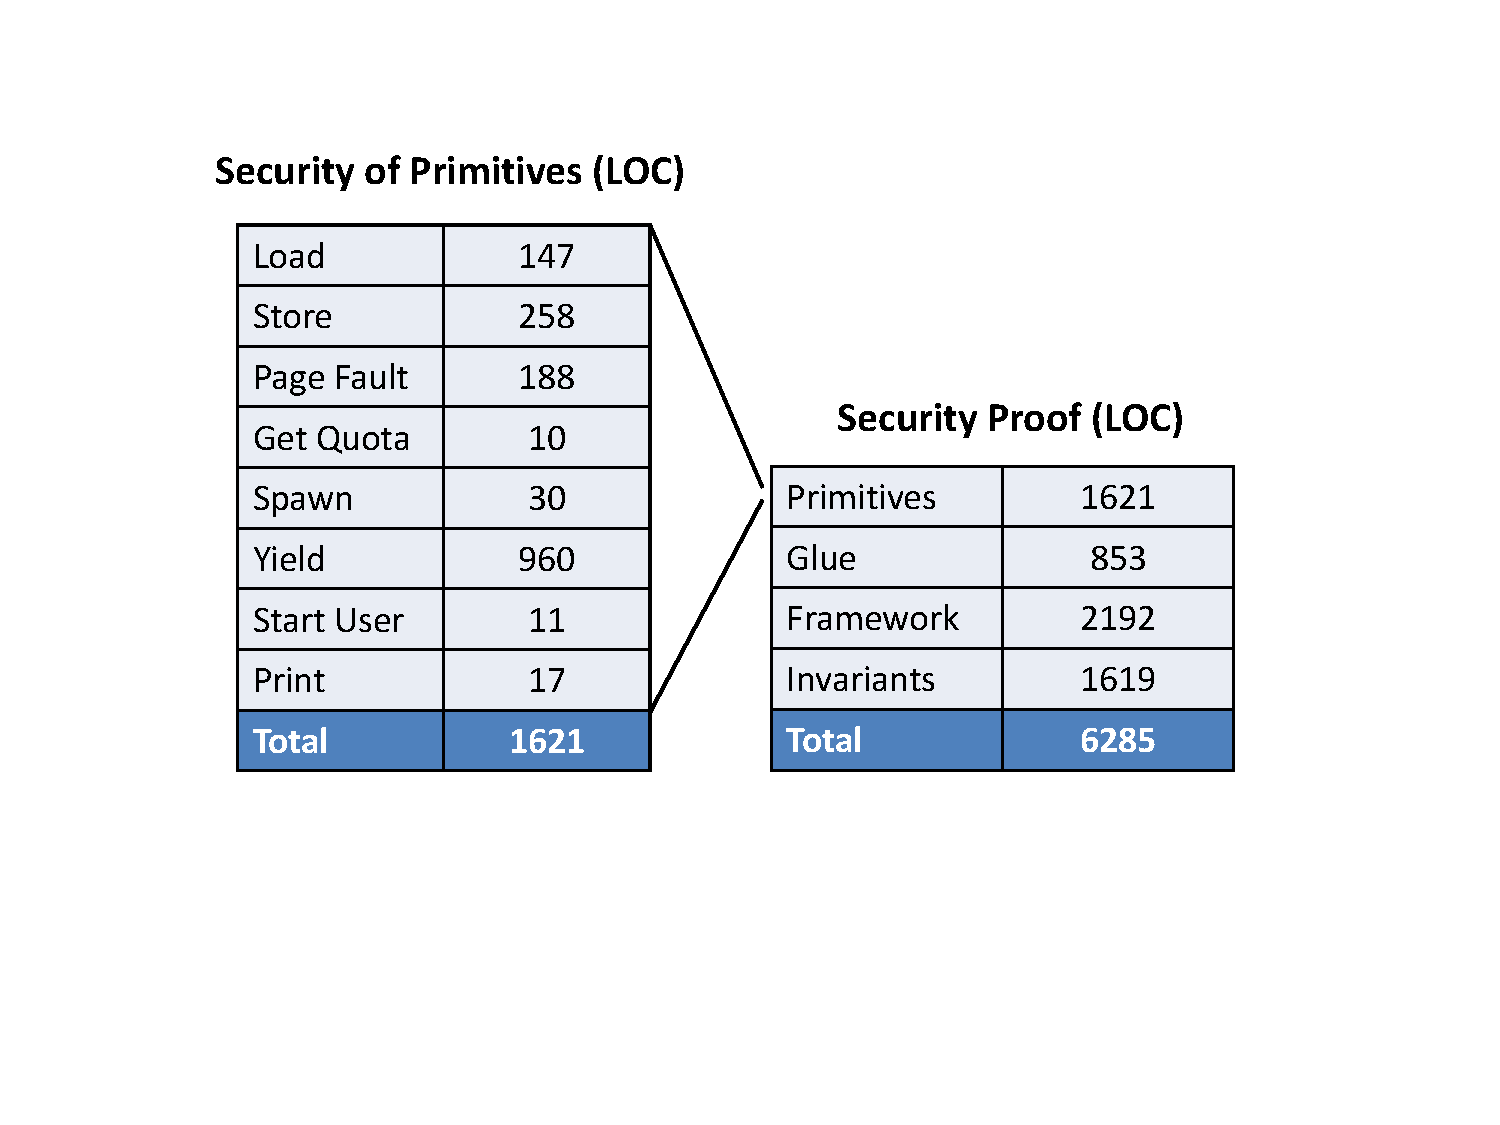
\includegraphics[scale=0.4]{pldi/figure/secure-loc.pdf}}
\caption{\small{Approximate Coq LOC of proof effort.}}
%\vspace*{-1.5ex}
\label{secure-loc}
\end{figure}

Figure~\ref{secure-loc} gives the number of lines of Coq definitions
and proof scripts required for the proof effort. 
The entire effort is broken down into security proofs for
primitives, glue code to interface the primitive
proofs with the LAsm$(L)$ semantics, definitions and proofs
of the framework described in Chapter~\ref{methodology-chapter}, and
proofs of new state invariants that needed to be established.
We will now discuss the most interesting aspects and difficulties 
of the TSysCall-local security proof.

\section{Conducting the TSysCall-local Security Proof}

%\vspace*{-1ex}
\paragraph{State Invariants}
%Some of the following descriptions of security proofs for
%primitives will refer to state invariants.
While mCertiKOS already verifies a number of useful state 
invariants, some new ones are needed for our security proofs.
%These invariants make up the 
%state predicate $I$ mentioned in the end-to-end security 
%theorem of Section~\ref{methodology}.
The most important new invariants established over 
TSysCall-local execution are:
\begin{enumerate}
\item In all saved register contexts, the instruction pointer 
register points to the entry of the 
\ttt{start\_user} primitive.
\item No page is mapped more than once in the page tables.
\item A user process is always either in user mode, or is in kernel mode 
and the instruction pointer register points to the entry of the \ttt{start\_user} 
primitive (meaning that the first part of yield was just executed,
and user mode will be restored in one step).
\item The sum of the available quotas (max quota minus usage) of all
spawned processes is less than or equal to the number of unallocated
pages in the heap (implying that page allocation will always be
successful if the process has quota available).
\end{enumerate}
\cut{
Additionally, for a given observer principal $p$, we assume the
invariant that process $p$ has been spawned. Anything occurring
before the spawning of $p$ is considered part of the 
initialization/configuration phase; we are not interested in 
reasoning about the security of process $p$ before the process
even exists in the system.}

%\vspace*{-1ex}
\paragraph{Security of Load/Store Primitives}
The main task for proving security of the $100$+ assembly commands
of LAsm(TSys\-Call) is to show that the TSysCall layer's load/store 
primitives preserve indistinguishability. This requires showing
that equality of virtual address spaces is preserved. Reasoning 
about virtual address spaces can get quite hairy since we always
have to consider walking through the page tables, with the 
possibility of faulting at either of the two levels.

To better understand the intricacies of this proof, consider the
following situation. Suppose we have two states $\sigma_1$ and
$\sigma_2$ with equal mappings of virtual addresses to option values
(where no value indicates a page fault). Suppose we are writing
to some virtual address $v$ in two executions on these states.
Consider what happens if there exists some other virtual address
$v'$ such that $v$ and $v'$ map to the same physical page
in the first execution, but map to different physical pages in
the second. It is still possible for $\sigma_1$ and $\sigma_2$
to have identical views of their virtual address space, as long
as the two different physical pages in the second execution
contain the same values everywhere. However, writing to $v$
will change the observable view of $v'$ in the first execution,
but not in the second. Hence, in this situation, it is possible
for the store primitive to break indistinguishability.

We encountered this exact counterexample while attempting to
prove security, and we resolved the problem by establishing
the second state invariant mentioned above. The invariant
guarantees that the virtual addresses $v$ and $v'$ will never 
be able to map to the same physical page, thus ruling
out the counterexample.

%%%%%%%%%%%%%%%%%%%%%%%%%%%%%%%%%%%%%%%%%%%%%%%%%%%%%%%%%%%%%%%%
\begin{figure}[t]
\begin{center}
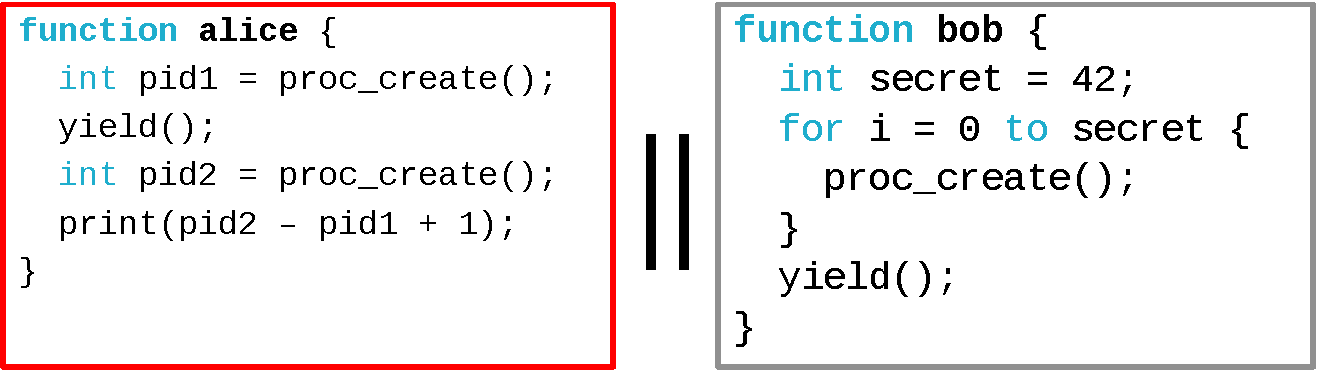
\includegraphics[scale=0.55]{pldi/figure/spawnleak}
\caption{\small Using child process IDs to as a side channel.}
\label{fig:proccreate-leak}
%\vspace*{-20pt}
\end{center}
\end{figure}
%%%%%%%%%%%%%%%%%%%%%%%%%%%%%%%%%%%%%%%%%%%%%%%%%%%%%%%%%%%%%%%%

%\vspace*{-1ex}
\paragraph{Security of Process Spawning}
During our verification effort, we discovered that the \ttt{proc\_create}
primitive had a major security flaw. Figure~\ref{fig:proccreate-leak} 
shows two user programs that exploit \ttt{proc\_create} as
a side channel for communication. When the insecure version of 
mCertiKOS creates a new child process, it chooses the lowest process 
ID not currently in use, and returns the ID to the user. 
\begin{comment}
\begin{alltt}
Alice:                       Bob:
  x = proc\_create();          yield(); 
  yield();                     for (i = 0; i < z; i++)
  y = proc\_create();            proc\_create();
  z = y - x - 1;               yield();
\end{alltt}
\end{comment}
In the figure, Alice spawns a child process, stores its 
ID into variable $x$, and then yields to Bob. Bob 
spawns a number of children equal to some secret value,
and then yields back to Alice. Finally, Alices spawns
another child, stores its ID into $y$, and observes the
value $y-x-1$. This observed value is exactly Bob's
secret!

To close this side channel, we had to revamp the way child
process IDs are chosen in mCertiKOS-secure. The new ID system 
works as follows. We define a global parameter $m$ limiting
the number of children any process is allowed to spawn.
Suppose a process with ID $i$ and $c$ children ($c < m$)
spawns a new child. Then the child's ID will always be
$i*m + c + 1$. This formula guarantees that different
processes can never interfere with each other via child
ID: if $i \neq j$, then the set of possible child IDs for
process $i$ is completely disjoint from the set of
possible child IDs for process $j$. It is easy to see how
this scheme closes the leak of Figure~\ref{fig:proccreate-leak}.
$x$ will always the contain the ID of Alice's first
child, while $y$ will contain the ID of Alice's second
child; these two values are determined solely by Alice's
own ID, so Bob is no longer capable of influencing them.

%\vspace*{-1ex}
\paragraph{Security of Page Fault}
\begin{comment}
There are two different interesting aspects of page-fault
security. The first is that it is a perfect example of 
a primitive whose implementation does not preserve
indistinguishability with each individual step. 
When a page fault occurs, 
either one or two new pages must be allocated from the global 
heap. Because all user processes use the same global heap for 
allocation, and mCertiKOS always allocates the first available
page, the physical address of an allocated page can potentially
leak information between processes. The page fault handler, however,
must make use of the physical address of a newly-allocated page
when inserting a new virtual address mapping into the page
table. Therefore, at some point during the actual (non-atomic)
execution of the page fault handler, an observable register contains
the insecure physical page address. Since we prove that the
primitive's atomic specification is secure, however, we know that
the insecure value must be overwritten by the time the
primitive finishes executing.
\end{comment}
Since page faults dynamically allocate new pages, security
of page faulting requires some reasoning about the resource quota 
implemented by containers (recall the container discussion in 
Chapter~\ref{casestudy-def-chapter}). More specifically, notice
that the global allocation table \ttt{AT} must be unobservable to
user processes since all processes can affect it via page allocation.
This means that the page fault handler may successfully allocate a page 
in one execution, but fail to allocate a page in an execution from
an indistinguishable state due to there being no pages available. 
Clearly, the observable result of the primitive will be different 
for these two executions. To deal with this difficulty, we relate available 
heap pages to available quota by applying the fourth state invariant 
mentioned above. Recall that the invariant guarantees that the sum 
of the available quotas of all spawned processes is always less than 
or equal to the number of available heap pages. Therefore, if an 
execution ever fails to allocate a page because no available page 
exists, the available quota of \emph{all} spawned processes must be 
zero. Since the available quota is observable, we see that allocation 
requests will be denied in both executions from indistinguishable
states. Therefore, we actually \emph{can} end up in
a situation where one execution has pages available for allocation 
while the other does not;
in both executions, however, the available quota will be zero, and
so the page allocator will deny the request for allocation.

%\vspace*{-1ex}
\begin{figure}
\centering{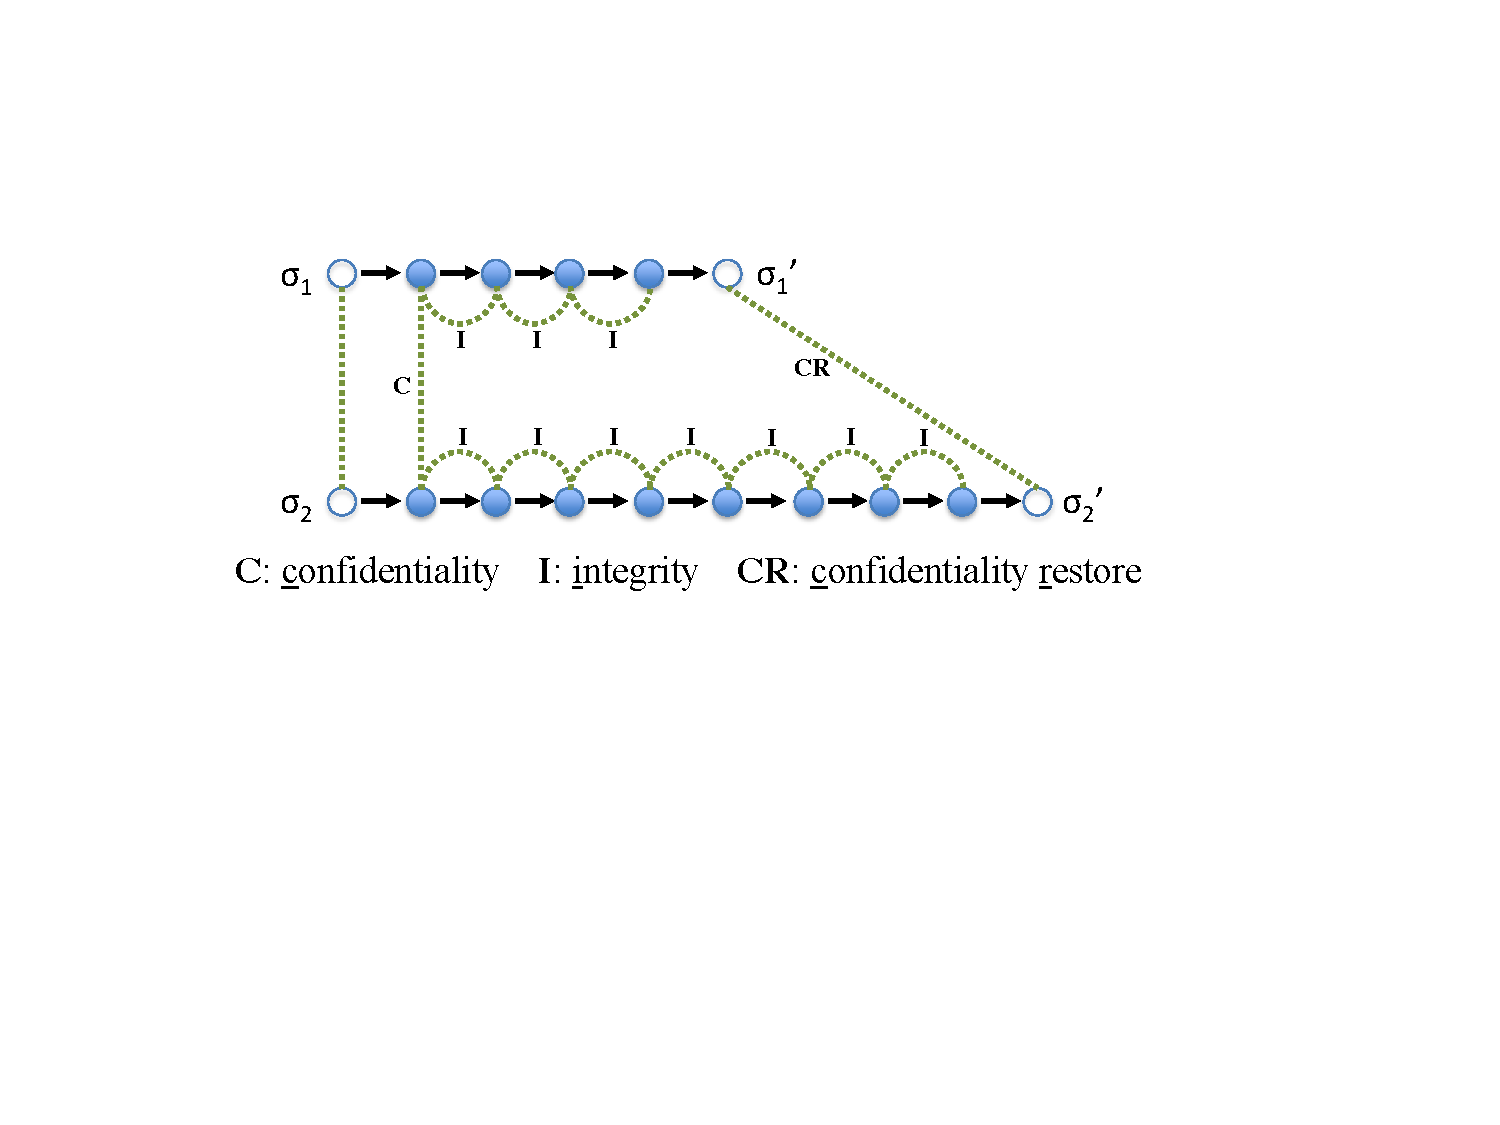
\includegraphics[scale=0.53]{pldi/figure/lemmas.pdf}}
\caption{\small Applying the three lemmas to prove the security
property of TSysCall-local yielding.}
%\vspace*{-3ex}
\label{bigstep-sec}
\end{figure}
\paragraph{Security of Yield}
Yielding is by far the most complex primitive to prove secure,
as the proof requires reasoning about the relationship between
the TSysCall semantics and TSysCall-local semantics. Consider
Figure~\ref{bigstep-sec}, where active states $\sigma_1$ and
$\sigma_2$ are indistinguishable, and they both call yield. 
The TSysCall-local semantics takes a big step over the executions 
of all non-observer processes;
these big steps are unfolded in Figure~\ref{bigstep-sec},
so the solid arrows are all of the individual steps of the 
TSysCall semantics. We must establish that a big-step yield
of the TSysCall-local machine preserves indistinguishability, 
meaning that states $\sigma_1'$ and $\sigma_2'$ in 
Figure~\ref{bigstep-sec} must be proved indistinguishable.
We divide this proof into three separate lemmas, proved over 
the TSysCall semantics:
\begin{itemize} \itemsep 0pt
\item \emph{Confidentiality}~--- If two indistinguishable
active states take a step to two inactive states, then those
inactive states are indistinguishable.
\item \emph{Integrity}~--- If an inactive state takes a step
to another inactive state, then those states are 
indistinguishable.
\item \emph{Confidentiality Restore}~--- If two indistinguishable
inactive states take a step to two active states, then those
active states are indistinguishable.
\end{itemize}
These lemmas are chained together as pictured in 
Figure~\ref{bigstep-sec}. The dashed lines indicate
indistinguishability. Thus the confidentiality lemma
establishes indistinguishability of the initial inactive
states after yielding, the integrity lemma establishes
indistinguishability of the inactive states immediately
preceding a yield back to the observer process, and the
confidentiality restore lemma establishes indistinguishability
of the active states after yielding back to the observer process.
%Therefore, these three lemmas together demonstrate that
%a big-step yield in the TSysCall-local machine preserves
%indistinguishability.

\ifextended
In the mCertiKOS proof, we actually generalize the confidentiality
lemma to apply to other primitives besides yield.
\begin{itemize}
\item \emph{Generalized Confidentiality}~--- Two indistinguishable
active states always take a step to indistinguishable states.
\end{itemize}
We frame all of the high-level security proofs for the other
primitives as instances of this confidentiality lemma. This
means that we derive high-level security of the entire TSysCall-local
machine by proving this generalized confidentiality lemma along with 
integrity and confidentiality restore.
\else\fi

Note that while the confidentiality and confidentiality restore
lemmas apply specifically to the yield primitive (since it is
the only primitive that can change active status), the
integrity lemma applies to all primitives.
Thus, like the security unwinding condition, integrity is proved 
for each of the TSysCall primitives. The integrity proofs are 
simpler since the integrity property only requires 
reasoning about a single execution, whereas security requires 
comparing two.

The confidentiality restore lemma only applies to the situation
where two executions are both yielding back 
to the observer process. The primary obligation
of the proof is to show that if the saved register contexts of two
states $\sigma_1$ and $\sigma_2$ are equal, then the actual registers
of the resulting states $\sigma_1'$ and $\sigma_2'$ are equal.
There is one interesting detail related to this proof:
a context switch in mCertiKOS does not save \emph{every} machine
register\maybecut{, but instead only saves those registers that are relevant
to the local execution of a process (e.g., EAX, ESP, etc.).}
In particular, the CR2 register, which the page fault handler
primitive depends on, is not saved. This means that, immediately
after a context switch from some process $i$ to some other process 
$j$, the CR2 register could contain a virtual address that is private 
to~$i$. How can we then guarantee that $j$ is not influenced by this
value? Indeed, if process $j$ is able to immediately call the page 
fault handler without first triggering a page fault, then it may very 
well learn some information about process $i$. We resolve this potential
leak by making a very minor change to mCertiKOS: we add a line of
assembly code to the implementation of context switch that clears
the CR2 register to zero.

\ifextended
\paragraph{Security of Other Primitives}

We do not need to reason about security of \ttt{proc\_init}
since we assume that initialization occurs appropriately,
and no process is ever allowed to call the primitive again after 
initialization finishes. None of the primitives \ttt{get\_quota}, 
\ttt{start\_user}, or \ttt{print} brought up any difficulties
for security verification.
\else\fi

\section{End-to-End Process Isolation}
\label{casestudy-isolation}

We conclude this chapter by taking a step back and revisiting the
top-level end-to-end security theorem. The final 
statement is the conclusion of Theorem~\ref{end-to-end}, which
is low-level security of the MBoot machine for all states
related by $\phi(M,p,I,R)$. In other words, the theorem says
that if we consider any MBoot state $s_1$ related to a
properly-initialized TSysCall state $\sigma_1$, and
we consider related modified states $s_2$ and $\sigma_2$
with $\sigma_2$ initialized and $\observe{p}{\sigma_1} = \observe{p}{\sigma_2}$, 
then the whole-execution behaviors of MBoot on $s_1$ and $s_2$
are identical. Notice that this statement requires a solid 
understanding of the particular mCertiKOS observation function. 
While it may feel intuitively clear that the observation function
defined in Section~\ref{ssec:security-overview} is reasonable,
how can we be certain? Poorly-defined observation functions are
certainly possible; for example, if we define an identity observation
function where all principals observe all program state, then 
the unwinding condition degenerates
into a simple statement of determinism. Thus applying our methodology
with such an observation function would not actually give us a result 
that is related to security.

In general, we consider the observation function definition to
be a trusted part of the methodology, in the same way that high-level
specifications must be trusted to actually specify our intuitive
desires for the software's behavior. However, depending on the
context, we may be able to do better than this. While we have not
yet completed a formal Coq development, we hope to prove a higher-level
end-to-end security theorem in mCertiKOS that truly guarantees 
user-process isolation by being completely independent from the choice 
of observation function. Our vision for how this would work involves
the following two steps:
\begin{enumerate}
\item Define a new state predicate $\spawned{p}$, saying that process
$p$ was \emph{just spawned} by the kernel. Prove that this predicate
is stronger than the initialization predicate $I$ 
(i.e., $\forall p \such \spawned{p} \Rightarrow I$).
\item Prove that \emph{all} states satisfying $\spawned{p}$ are
indistinguishable from one another according to $p$
(i.e., $\forall \sigma_1, \sigma_2 \in \spawned{p} \such 
\observe{p}{\sigma_1} = \observe{p}{\sigma_2}$). We imagine that
such a property should be provable since all of $p$'s data should
be in a deterministic initial state (e.g., all zeros) immediately 
after $p$ is spawned.
\end{enumerate}
Assuming we can successfully implement these steps, the end-to-end
security guarantee can clearly be reformulated as follows: if we consider
some MBoot state $s_1$ that is related to a TSysCall state $\sigma_1$
which occurs immediately after $p$ is spawned (i.e., $\sigma_1 \in \spawned{p}$), 
along with related modified states $s_2$ and $\sigma_2$ (with
$\sigma_2 \in \spawned{p}$), then the 
whole-execution behaviors of MBoot on $s_1$ and $s_2$ are identical.
With this theorem formulation, we no longer need to understand and
trust the choice of observation function. While we still have some
details to work out, we are hopeful that such a theorem can be 
established in the near future.




\chapter{New Feature: Virtualized Time}
\label{timing-chapter}

To demonstrate the extensibility of our methodology, we
decided to add a new, useful feature to mCertiKOS-secure:
the ability for user processes to time their own executions.
Timing flows pose a notoriously difficult challenge for
security reasoning. Nevertheless, we were able to successfully
implement and verify the security of this new feature with
only about two person-weeks of effort. The generality of the
observation function is extremely helpful for clearly specifying
how user processes view time.

%%%%%%%%%%%%%%%%%%%%%%%%%%%%%%%%%%%%%%%%%%%%%%%%%%%%%%%%%%%%%%%%
\begin{figure}[t]
\begin{center}
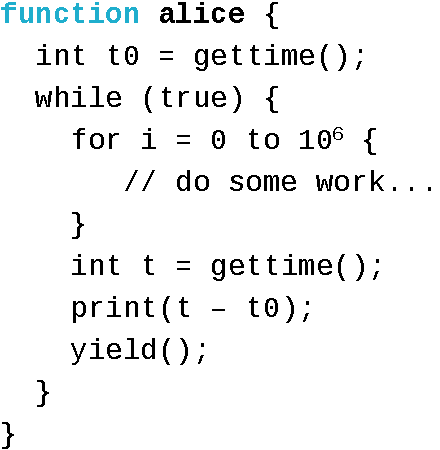
\includegraphics[scale=0.55]{pldi/figure/gettime}
\caption{\small A sample usage of the \gett{} feature.}
\label{fig:gettime}
%\vspace*{-20pt}
\end{center}
\end{figure}
%%%%%%%%%%%%%%%%%%%%%%%%%%%%%%%%%%%%%%%%%%%%%%%%%%%%%%%%%%%%%%%%

\section{Specification and Implementation of Timing}
Figure~\ref{fig:gettime} shows a motivating example for the
new feature that we would like to support. We wish to
provide a system call \gett{} that user processes
can invoke to help time their executions. However, we do
not want to allow processes to communicate with each other
by exploiting this timestamp. Hence we must create some notion
of \emph{virtualized} time, whereby each process has its
own isolated timeline.
It is important to note that the feature we are implementing
here is completely orthogonal to a wall-clock time. While
a user can observe the time of an event within the context of
his own timeline, our threat model still assumes that he has
no mechanism for associating that event with a global
wall-clock time.

\paragraph{TSC Oracle}
As a basis for implementing the timing feature, we make use of 
x86's Time Stamp Counter (TSC), which keeps track of the total
number of clock cycles since the last reset. At the machine model
level (MBoot), we add a new primitive \ttt{rd\_tsc}, and axiomatize
its specification. The primitive's implementation is unverified
but extremely simple: it looks up the current TSC value using
x86's RDTSC instruction, and returns the value. Note that the
TSC value clearly can be used as a potential information-flow
side channel; thus the \ttt{rd\_tsc} primitive is not exposed to
users at the TSysCall level, and users are not allowed to directly
invoke the RDTSC instruction (x86 has a global TSD flag which, 
when set, will cause a user-mode RDTSC invocation to trigger
an exception).

Defining the specification of \ttt{rd\_tsc} is somewhat subtle.
We certainly do not want to model the actual number of cycles on
the machine, since this is highly nondeterministic. A single
assembly instruction could take any number of cycles to
execute depending on various unpredictable conditions. Rather
than try to accurately specify the value of the TSC, we will instead assume 
the existence of an \emph{oracle} for a given execution that will 
accurately answer the question, ``for any $n$, what is the TSC 
value returned by the $n$th invocation of the RDTSC instruction?''
This strategy is reasonable because of the following two facts:
(1) our theorems will apply to \emph{any} choice of oracle; and 
(2) for every actual execution, there exists some oracle consistent 
with that execution.

%%%%%%%%%%%%%%%%%%%%%%%%%%%%%%%%%%%%%%%%%%%%%%%%%%%%%%%%%%%%%%%%
\begin{figure}[t]
\begin{center}
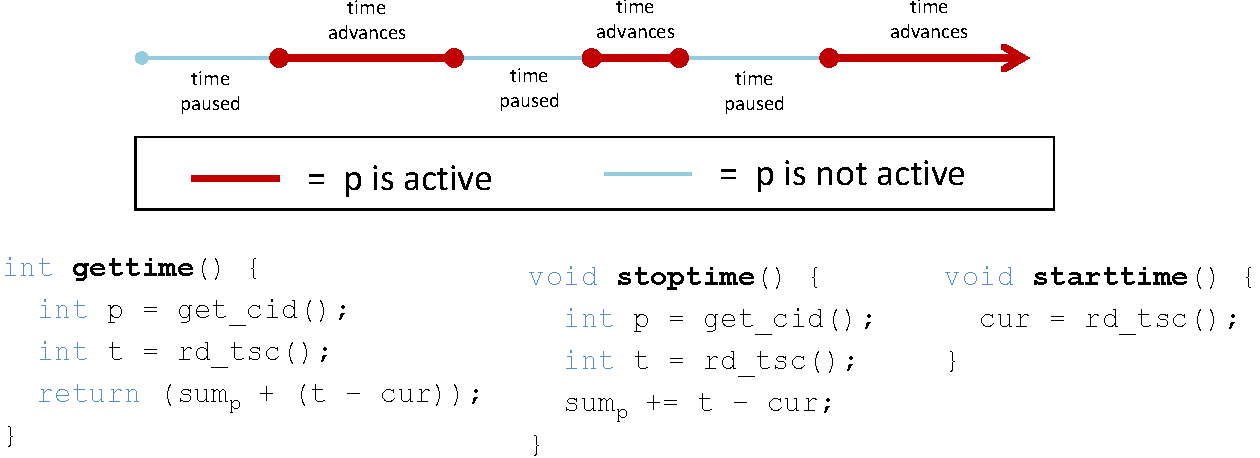
\includegraphics[scale=0.685]{pldi/figure/timeline}
\caption{\small Illustration and implementation of local timelines.}
\label{fig:timeline}
%\vspace*{-20pt}
\end{center}
\end{figure}
%%%%%%%%%%%%%%%%%%%%%%%%%%%%%%%%%%%%%%%%%%%%%%%%%%%%%%%%%%%%%%%%

\paragraph{Local Timeline}
Given our specification of the physical TSC in terms of an oracle,
we virtualize the TSC value for each user process by implementing
isolated timelines. Figure~\ref{fig:timeline} illustrates a
timeline that is local to process $p$, and shows the code that
implements all timelines. It is useful to think of our
implementation in terms of stopwatches. Each process has its
own stopwatch: \gett{} returns the value of the active
(i.e., currently-running) process's stopwatch, \stopt{}
pauses the active process's stopwatch, and \startt{} resumes
the active process's stopwatch. Whenever a process yields,
\stopt{} is called prior to context switching, the active 
process ID is changed to be
the head of the ready queue, and finally \startt{} is called after context 
switching. This
guarantees that, at any given moment during execution, all 
process's stopwatches are paused except for the active one.

The code of Figure~\ref{fig:timeline} shows a straightforward
way to implement these stopwatches. In the following, we will
use the term \emph{epoch} to refer to a portion of execution
in between two consecutive yields. We say that an epoch belongs
to process $p$ if $p$ is the active process during that epoch.
At any moment during an execution, we use the term 
\emph{current epoch} to refer to the portion of execution since
the most recent yield. Given this terminology, the stopwatch 
implementation uses the following two fields of program state:
\begin{itemize}
\item $\ttt{sum}_i$~--- For each process $i$, this integer value 
gives the total amount of time spent in previous completed epochs
belonging to $i$.
\item \ttt{cur}~--- This integer value records the TSC value of the
beginning of the current epoch.
\end{itemize}
Given these fields, the current virtualized time at any moment
can be computed as $\ttt{sum}_p + (t - \ttt{cur})$, where $p$ is the
active process and $t$ is the current TSC value returned by \ttt{rd\_tsc}. 
Whenever a yield occurs, the appropriate \ttt{sum} is 
increased by the length of the just-completed epoch (\ttt{stoptime}), and 
then \ttt{cur} is reset to the current TSC value (\ttt{starttime}). In this 
way, each process has its own virtualized timeline.

\paragraph{Aside on TSC Overflow}
Technically, we need to be concerned with errors in our code arising
from the TSC value overflowing. However, the TSC is a 64-bit value 
in x86 architecture, so a machine would have to be running for
well over a century on modern architecture in order for overflow
to occur. Therefore, we choose to embed an assumption within our
verification that the return value of \ttt{rd\_tsc} is always
less than $2^{64}$. Notice that this assumption implies that
the virtualized time $\ttt{sum}_p + (t - \ttt{cur})$
also does not overflow, since this value is a subset of the
timeline interval from 0 to $t$.

\section{Security of Virtualized Time}
The generality of the observation function allows for a clean and
simple security verification of virtualized time. For convenience,
we first add a field \ttt{tsc} to abstract state that represents 
the physical TSC. It gets updated to the return value of \ttt{rd\_tsc}
whenever that primitive is called. In other words, \ttt{tsc} simply
remembers the value that \ttt{rd\_tsc} returned the last time it 
was called. Given this, we define three timing-related observations made 
by process $p$:
\begin{itemize}
\item \emph{Previous Epochs}~--- The value of $\ttt{sum}_p$ is observable.
\item \emph{Current Epoch}~--- The value of ($\ttt{tsc} - \ttt{cur}$) is 
observable if $p$ is the active process.
\item \emph{Oracle}~--- The $p$-filtered subset of the TSC oracle is 
observable (discussion below).
\end{itemize}
The first two observations clearly imply that the virtualized time
$\ttt{sum}_p + (t - \ttt{cur})$ is always observable when
$p$ is the active process and $t$ is the value just returned by
\ttt{rd\_tsc}; this fact yields a simple security proof
of the \gett{} system call. Notice how we exploit generality of the
observation function here by making the difference between \ttt{tsc}
and \ttt{cur} observable, even though each of the two values individually
must be unobservable since they pinpoint timestamps on a \emph{global}
timeline rather than local.

%\noindent
The third observation is quite subtle. Consider the following 
two insights:
\begin{enumerate}
\item \emph{The oracle cannot be entirely unobservable.}
Recall that the specification of \gett{} first
sets $t$ to be the next value given by the oracle, and then 
returns $\ttt{sum}_p + (t - \ttt{cur})$. 
In order to prove that this specification is noninterfering,
we must know that the oracle produces the same $t$ value
in two indistinguishable states. Therefore the oracle cannot
be entirely hidden from observation.
\item \emph{The oracle cannot be entirely observable.} 
It is possible that in two executions
from indistinguishable states, a process $p'$ which is not the 
observer $p$ may invoke \gett{} a different number of times, implying
an information flow from $p'$ to $p$. In other words, the 
integrity lemma of Chapter~\ref{casestudy-proof-chapter} will
fail to hold if the entire oracle is observable to~$p$,
since other processes can clearly change the oracle by invoking
\gett{}.
\end{enumerate}
Together, these insights imply that only some portion of the
oracle can be observable to~$p$. In particular, we need to
somehow filter the oracle, observing only those entries
which correspond to \ttt{rd\_tsc} invocations made by $p$.
One potential solution would be to divide the single global
oracle into many per-process oracles. Unfortunately, this
solution makes it difficult to define the semantics of
\ttt{rd\_tsc} at the MBoot level. At the TSysCall level, we
would choose which oracle to query based on the currently-running
process, stored in the abstract data field \ttt{cid}; at the
MBoot level, however, \ttt{cid} has not yet been abstracted.
It might be possible to specify the MBoot-level semantics to
inspect the concrete memory corresponding to \ttt{cid}, but this
would cause all kinds of trouble since it would violate the mCertiKOS 
convention that primitive specifications never depend on concrete 
memory.

Instead, we use a simple solution that cleverly exploits our
assumption of safety of the high-level machine (the first
property of Definition~\ref{high-level-security} in 
Chapter~\ref{methodology-chapter}). For each natural
number $n$, we extend the oracle to return not only the
current TSC value, but also an integer $p$ representing a process
ID. At the TSysCall level, $p$ is used as a prerequisite for safe
execution: the specification of \gett{} checks whether $p$ is
equal to \ttt{cid}, and returns \none{} if this check fails.
At the MBoot level, on the other hand, $p$ is completely ignored
by the \ttt{rd\_tsc} specification, allowing us to define the
specification without a need to refer to \ttt{cid}. This means that there are
some oracles for which a TSysCall-level execution gets stuck, but
the corresponding MBoot-level execution is safe. Thankfully, this 
odd situation is irrelevant due to the fact that we assume safe
execution at the TSysCall level as a prerequisite for all of our
major theorems. Notice that
this solution is still justifiable in the following sense: even
though many choices of oracle will now yield faulty high-level 
execution, there still always exists some valid oracle for any 
actual, safe execution.

Given this extended definition of oracle, we can now 
$p$-filter an oracle by choosing only those entries with process
ID~$p$. Then, as mentioned above, we make only this $p$-filtered
oracle subset observable to~$p$. While the intuitive concept should
be clear at this point, the technical details of defining 
$p$-filtering are actually still a bit tricky. Because we represent
the oracle as a function from natural numbers to pairs, we also
keep track of the current natural-number position in abstract state.
Whenever \ttt{rd\_tsc} is called, this position is incremented
by one. When defining the observation, we must be careful how we
treat this oracle position, since it could be a source of information leak.
To make observability independent from the precise value of the oracle 
position, we define a function \ttt{filter}$(o,c,p,n)$ which takes oracle 
$o$, oracle position $c$, process ID $p$, and natural number $n$ as parameters, 
and returns the $n$th occurrence of pairs in $o$ with process ID equal
to $p$, starting from position $c$. Then oracle observation is defined 
as:
\[\observe{p}{\sigma} \isdef \lambda~n \such \ttt{filter}(\ttt{oracle}(\sigma),
\ttt{oracle\_pos}(\sigma),p,n)\]
In other words, rather than make the oracle position $c$ 
observable, we make the infinite stream of $p$-related
oracle entries starting from $c$ observable. 

With the help of a few simple lemmas characterizing this 
\ttt{filter} function, the entire security verification of virtualized 
time goes through quite easily. The generality of the observation
function is key in allowing us to prove security of this new kernel feature.
This clearly demonstrates the extensibility of our novel methodology: even 
though we need to introduce the concept of an oracle for reasoning about
time within mCertiKOS, the timing-sensitive security verification
is still completely straightforward.







\chapter{Assumptions, Limitations, and Future Work}
\label{limitations-chapter}

We have demonstrated that our new methodology is extremely
general, and is effective in guaranteeing security of realistic,
low-level systems code. Nevertheless, like any framework, it
has its fair share of assumptions and limitations. In this 
chapter, we discuss the most important limitations in order to 
help contextualize the situations in which our methodology
should or should not be applicable.

\paragraph{Fidelity of the Assembly Machine Model}
Our methodology only yields a security proof for assembly
programs that fit within our model of x86 assembly execution. The
model is an extended version of CompCert's, primarily designed
for supporting all of the features needed by the mCertiKOS
kernel implementation (e.g., distinction between kernel and
user mode executions). We make no claims about the relationship
between our model and the physical hardware that executes x86 
assembly code. If one wished to apply our proof to the actual
machine execution, the following significant gaps would need
to be closed:
\begin{itemize}
\item \emph{Completeness Gap}~--- Our model is certainly not complete for
all user-level assembly programs, so it may be possible to violate 
security on actual hardware by exploiting unmodeled assembly 
instructions. One example of such an instruction is RDTSC,
which reads the x86 timestamp counter, as described in 
Chapter~\ref{timing-chapter}. The TSC can be used as a communication
channel between processes, leaking information about how much
time certain processes have spent executing. We do not model the
RDTSC instruction~--- a user program that uses the instruction
would not even be considered valid syntax in our model, so there is
no way that any verified properties could apply to such a program.
Note that even in the extension described in Chapter~\ref{timing-chapter},
we choose not to model the RDTSC instruction; instead, we axiomatize
a \ttt{rd\_tsc} primitive and call the RDTSC instruction in its 
unverified implementation.

\item \emph{Soundness Gap}~--- In addition to this completeness gap, there is 
also a potential soundness 
gap between our machine model and the physical hardware; we must trust that 
the semantics of all of our modeled assembly instructions are faithful to
the actual hardware execution. This is a standard area of trust that arises
in any formal verification effort: at some point, we always reach a low-enough 
level where trust is required, whether this means trusting the operating system that 
a program is running on, trusting the hardware to meet its published specifications, 
or trusting the laws of physics that the hardware is presumably obeying. Note
that the level of trustworthiness of our machine model is similar to CompCert's, 
since we use a modest extension over CompCert's model.

\item \emph{Safety Gap}~--- The soundness gap just described requires us 
to trust that whenever the
modeled semantics of an assembly instruction is well-defined, the execution
of that instruction on physical hardware will do what the model says. What
happens, however, if the modeled semantics gets stuck? The model makes
no promises about the actual execution of a stuck semantics; the 
execution could continue running without issues, but it would no longer
be bound by any of our verification. Therefore, even if we closed the 
completeness and soundness gaps described above to a point of satisfaction, 
we would still be required to assume that user programs never have undefined 
semantics in order to apply our verification to the physical execution.
This is quite a heavyweight assumption, as user-level code is meant to 
represent arbitrary and unverified assembly.
\end{itemize}

\paragraph{Future Plans for Model Fidelity}
In light of these various unrealistic assumptions required to apply our
verification to the physical machine, it would be desirable to implement
a clearer and more streamlined representation of user-mode assembly 
execution. The mCertiKOS assembly model was designed for verification
of the kernel code; there is actually no need to use that model for unverified
user process execution. Instead, we can design a simple model consisting
of registers and a flat memory representing a virtual address space, where
an instruction can be one of the following:
\begin{itemize}
\item \emph{interrupt}~--- A trap into the kernel to handle, for example, 
a privileged instruction or a system call.
\item \emph{load/store}~--- Instructions that use the kernel's load/store
primitives to access the virtual address space. These may trigger a page 
fault, to be handled by the kernel.
\item \emph{other}~--- Any other user-land instruction, which is assumed
to only be able to read/write the values in registers.
\end{itemize}

This simple model has the benefit of making very clear exactly what 
assumption needs to hold in order to relate the model to actual execution:
the arbitrary user-land instructions must only depend upon and write
values in the modeled registers. Notice that the RDTSC instruction
described above is an example of an instruction that does \emph{not}
satisfy this assumption; hence it would need to be explicitly modeled
if we wanted to support it.

We hope that future work can gradually model more and more hardware 
features and instructions like RDTSC that do not satisfy this assumption.
Each new feature could potentially violate security, and thus will 
require some additional verification effort. For the RDTSC example, we
would close the timestamp counter information channel by setting the
timestamp disable flag (TSD), which causes the hardware to treat
RDTSC as a privileged instruction. Then, if a user process attempts to 
execute the instruction, the hardware will generate an exception and 
trap into the kernel. The kernel will then handle the exception in a way
that is verified to be secure (e.g., it could kill the process, 
yield to a different process, or return a virtualized timestamp as
in Chapter~\ref{timing-chapter}).

\paragraph{High-Level Policy Specification}
As with any formal verification effort, we must trust that the top-level 
specification of our system actually expresses our intentions for the system, 
including the security policy specified as 
an observation function. Because observation functions can have any type, 
our notion of security is far more expressive than classical pure 
noninterference. This does mean, however, that it can potentially be 
difficult to comprehend the security ramifications of a complex or 
poorly-constructed observation function. We place the onus on the system
verifier to make the observation function as clear and concise as 
possible. This view is shared by a number of previous security frameworks
with highly-expressive policy specification, such as the PER 
model~\cite{sabelfeld99} and Relational Hoare Type Theory~\cite{rhtt}.
In our mCertiKOS security specification, the virtual address space
observation provides a good example of a nontrivial but
clear policy specification~--- hiding physical addresses is, after all,
the primary reason to use virtual address spaces. Note, however,
as we discussed in Section~\ref{casestudy-isolation}, it may actually
be possible to remove this trust requirement in certain contexts by
proving a higher-level theorem that is independent from the choice
of observation function.

\paragraph{Applicability of the Methodology}
In order to utilize our security methodology, the following steps must be taken:
\begin{itemize}
\item The high-level security policy must be expressed as isolation
  between the observation functions of different principals. As
  mentioned previously, the complete lack of restrictions on the
  observation function yields a very high level of policy
  expressiveness. While a systematic exploration of expressiveness
  remains to be done, we have not encountered any kinds of information
  flows that are %obviously inexpressible
  not expressible in terms of an observation function.

\item The high-level security property
  (Definition~\ref{high-level-security}) must be provable over the
  top-level semantics. In particular, this means that
  indistinguishability must be preserved on a step-by-step basis. If
  it is not preserved by each individual step, then the top-level
  semantics must be abstracted further. For example, in our mCertiKOS
  security verification, we found that the TSysCall semantics did not
  preserve indistinguishability on a step-by-step basis; we therefore
  abstracted it further into the TSysCall-local semantics that hides
  the executions of non-observer processes.  We are unsure if this
  requirement for single-step indistinguishability preservation could
  be problematic for other systems. In our experience, however,
  repeated abstraction to the point of atomicity is highly desirable,
  as it yields a clear specification of the system.

\item Indistinguishability-preserving simulations must be established
  to connect the various levels of abstraction. While the main
  simulation property can require significant effort, we have not
  found the indistinguishability preservation property to be difficult
  to establish in practice. The property generally feels closer to a
  sanity check than a significant restriction. Consider, for instance,
  the example of the \ttt{swap} primitive from
  Section~\ref{informal-simulation}.  That example failed to preserve
  security across simulation because the local variable \ttt{z} was
  being considered observable. A caller of the \ttt{swap} primitive
  should obviously have no knowledge of \ttt{z}, however. Thus this is just a
  poorly-constructed observation function; a reasonable notion of
  observation would hide the local variable, and indistinguishability
  preservation would follow naturally.
\end{itemize}

\paragraph{User Process Safety}
There are a number of assumptions required specifically for the mCertiKOS
security guarantee (as opposed to the general theory). Most of these are 
directly inherited from the mCertiKOS
soundness theorem, such as correctness of the bootloader, device drivers,
and the CompCert assembler; see~\cite{certikos-popl} for more details on
these assumptions. There is, however, one new assumption that requires 
discussion here, related to the safety of user processes.

Notice that the theory presented in Chapter~\ref{methodology-chapter} 
requires a proof of safety of the 
top-level semantics, with respect to some initialization invariant $I$ 
(Definition~\ref{high-level-security}). This means 
we must prove that $I$ is preserved by each individual step of the 
semantics, and that the semantics can always take a step from any state
satisfying $I$ (i.e., standard preservation and progress properties).
We have a proof of preservation for mCertiKOS, but not progress.
The current version of mCertiKOS is non-preemptive 
and trusts user processes to have well-defined semantics. The TSysCall-local
semantics can thus get stuck in either of the following ways:
\begin{itemize}
\item The semantics does not currently specify what should happen when a 
user process attempts to execute an assembly instruction that has 
undefined semantics, such as a division by zero. Ideally, an operating system 
should provide a sandbox environment for user processes, where any undefined 
instruction causes a trap into the kernel, and is handled by either killing the
offending process or by yielding to a different process. mCertiKOS does not yet 
do this, but we hope this could be done in future work.
\item The big steps of the TSysCall-local semantics (Figure~\ref{bigstep}) could 
get stuck if a process yields but is never scheduled again. Even if we proved 
that the kernel scheduler is fair (which would not be difficult as it currently 
only does round-robin scheduling), we would still need to assume that user 
processes always eventually call yield. This is a fundamental limitation of a 
non-preemptive kernel. There are plans to make mCertiKOS preemptive in the 
future, but this requires a significant amount of effort.
\end{itemize}
Because of this potential for the top-level semantics to get stuck, we assume 
a significant hypothesis in our Coq proof, which essentially says that neither of
the two situations above ever happens. While this hypothesis is necessary
at the moment, it can be completely discharged if mCertiKOS is upgraded 
with a sandbox feature and preemption.

\paragraph{Inter-Process Communication}
The mCertiKOS verification presented in this work only applies to a version of 
the kernel that disables IPC. In the future, we would like to allow some 
well-specified and  disciplined forms of IPC that can still be verified 
secure. We have actually already started adding IPC~--- our most recent version of 
the secure kernel includes an IPC primitive that allows communication between all
processes with ID at most $k$ (a parameter that can be modified). The
security theorem then holds for any observer process with ID greater
than $k$. Ideally, we would like to extend this theorem
so that it guarantees some nontrivial properties about those
privileged processes with low ID.
   




\chapter{Related Work and Conclusions}
\label{related-chapter}

\section{Locality in Separation Logic}
\label{related-bpsl}

The definition of locality (or local action), which enables the frame
rule, plays a critical role in Separation
Logic~\cite{io00,reynolds02,yang:fossacs02}. Almost all versions of 
Separation Logic~--- including their
concurrent~\cite{brookes:concur04,ohearn:concur04,coy07},
higher-order~\cite{birkedal05}, and relational~\cite{yang07} variants,
as well as mechanized implementation (e.g., \cite{appel07})~--- have always used
the same locality definition that matches the well-known Safety and
Termination Monotonicity properties and the Frame
Property~\cite{yang:fossacs02}. 

In Chapter~\ref{bpsl-chapter}, we argued a case for strengthening the definition of locality 
to enforce \emph{behavior preservation}. This means that the behavior of a
program when executed on a small state is identical to the behavior when
executed on a larger state~--- put another way, excess, unused state cannot have
any effect on program behavior. We showed that this change can be made to have
no effect on the usage of Separation Logic, and we gave multiple examples of
how it simplifies reasoning about metatheoretical properties. 

\paragraph{Determinism Constancy}
One related work that calls for comparison is the property of
``Determinism Constancy'' presented by Raza and Gardner~\cite{rg09}, which
is also a strengthening of locality. While they use a slightly different notion 
of action than we do, it can be shown that Determinism Constancy, when translated
into our context (and ignoring divergence behaviors), is logically equivalent to:
\begin{align*}
\relate{\den{C}}{\sigma_0}{\sigma_0'} \land \sigma_0' \# \sigma_1 \Longrightarrow 
  \sigma_0 \# \sigma_1 \land \relate{\den{C}}{(\sigma_0 \dt \sigma_1)}{(\sigma_0' \dt \sigma_1)}
\end{align*}
\noindent{}For comparison, we repeat our Forwards Frame Property here:
\begin{align*}
\relate{\den{C}}{\sigma_0}{\sigma_0'} \land \sigma_0 \# \sigma_1 \Longrightarrow 
  \sigma_0' \# \sigma_1 \land \relate{\den{C}}{(\sigma_0 \dt \sigma_1)}{(\sigma_0' \dt \sigma_1)}
\end{align*}
While our strengthening of locality prevents programs from increasing state during
execution, Determinism Constancy prevents programs from \emph{decreasing} state.
The authors use Determinism Constancy to prove the same property regarding footprints
that we proved in Section~\ref{ssec:footprint}. Note that, while behavior preservation
does not imply Determinism Constancy, our concrete logic of Section~\ref{concrete} does
have the property since it never decreases state (we chose to have the \freee{} command put the 
deallocated cell back onto the free list, rather than get rid of it entirely).

While Determinism Constancy is strong enough to prove the footprint property, it does
not provide behavior preservation~--- an execution on a small state can still become
invalid on a larger state. Thus it will not, for example, help in resolving the dilemma 
of growing relations in the data refinement theory of~\cite{filipovic10}. Due to the lack of behavior 
preservation, we do not expect the property to have a significant impact on the metatheory
as a whole. Note, however, that there does not seem to be any harm in using \emph{both}
behavior preservation and Determinism Constancy. The two properties together enforce that
the area of memory accessible to a program be constant throughout execution.

\paragraph{Module Reasoning}
Besides our discussion of data refinement in
Section~\ref{ssec:datarefinement}, there has been some previous work
on reasoning about modules and their implementations within
the context of Separation Logic. In~\cite{oyr04},
a ``Hypothetical Frame Rule'' is used to allow modular reasoning when
a module's implementation is hidden from the rest of the
code. In~\cite{birkedal05}, a higher-order frame rule is used to allow
reasoning in a higher-order language with hidden module or function
code. However, neither of these works discuss relational reasoning
between different modules. We are not aware of any relational logic
for reasoning about modules.

\ifextended
Section~\ref{metatheory-security} discussed how behavior 
preservation is fundamentally important for combining local
reasoning with security verification; one interesting area
for future work would be to formalize this relationship
in the context of mCertiKOS. Currently, mCertiKOS uses a
single monolithic datatype for abstract state. In the future,
the framework could be altered to instead divide abstract
state into minimal composable pieces. This would yield clea
primitive specifications that only operate over the portion
of abstract state needed by the primitive (e.g., the \ttt{get\_quota}
specification would only take the \ttt{container} portion of abstract 
state as input). Behavior preservation would then need to be
explicitly enforced in order to \emph{soundly} and \emph{securely} combine 
all of these ``small'' specifications into a single, system-wide guarantee.

\begin{comment}
Another direction for future work would be to define a
behavior-preserving version of Concurrent Separation Logic that has
the same inference rules as standard CSL. The commands that acquire
and release locks should be able to be expressed in a
behavior-preserving fashion by including both local and shared state
in the underlying state model. A lock acquire will move memory from
the shared state into the local state, while a lock release will move
it from local into shared. Neither command requires an increase in
total state. The model could get quite interesting if we allow threads
to allocate memory. One possible way to implement this might be to
assign a separate free list to each thread. Another way might be to
use a single free list, and, at any point in execution, we consider
the free list to be owned by the currently-executing thread.
\end{comment}
\fi

\section{Security-Aware Program Logic}
\label{related-ddifc}

%There are many different systems for reasoning about information flow. 
%We will briefly discuss some of the more closely-related ones here.

%Some IFC systems with declassification, such as Hi-Star~\cite{histar}, Flume~\cite{flume},
%and RESIN~\cite{resin}, reason at the operating system or process level, rather than the language 
%level. These systems can support complex security policies, but their formal
%guarantees suffer due to how coarse-grained they are. 

\begin{comment}
Hi-Star~\cite{histar} is a security-aware operating 
system that tracks and propagates security labels on processes and files. Processes with a special
declassification privilege are allowed to perform certain declassifications. We are not aware of any
formal, end-to-end noninterference guarantee for Hi-Star. 

Flume~\cite{flume} takes many ideas from Hi-Star, places them in
a more formalized and abstract setting, and provides a cleaner label model and declassification 
system. A process-level pure noninterference theorem is proved when no process with declassification 
privileges is being executed. However, Flume is forced to assume the worst about any process that
does have declassification privileges since it does not know the process's underlying code. A process
with the privilege to declassify Alice's data must be completely trusted by Alice. This is similar to
our notion of isolated method, except that the trusted base is only a few lines of code, rather than
the entirety of the code being executed by the trusted process. Additionally, our system allows for
some declassification to occur without an explicit declassification command being used~--- this kind
of declassification does not require any trusted code at all.

RESIN~\cite{resin} is actually more of a combination between an OS-level and a language-level IFC 
system. If a process needs to declassify some data, it must pass the data through a policy object.
This policy object is much like our notion of isolated method in that it contains some
trusted code (usually just a few lines) that releases the high-security data. The object also comes
with some metadata describing the conditions under which the declassification can be performed.
This metadata describes a declassification policy, in the same way that labels being conditioned
on state predicates describe a policy in our system. The primary difference between the systems is
that RESIN does not provide any formal security guarantee. We would thus imagine that, after
adding appropriate extensions to our system, we could formally verify the security of some 
programs implemented in RESIN.
\end{comment}

In the area of language-based IFC reasoning~\cite{sabelfeld03}, there are many type systems 
and program logics that share similarities with our logic presented in Chapter~\ref{logic-chapter}.

Amtoft et al.~\cite{amtoft06} develop a program logic for proving noninterference of 
a program written in a simple object-oriented language. They use relational assertions
of the form ``$x$ is independent from high-security data.'' Such an assertion is equivalent
to saying that $x$ contains \lo{} data in our assertion language. Thus their logic can be used to prove
that the final values of low-security data are independent from initial values of high-security
data~--- this is pure noninterference. Note that, unlike our logic, theirs does not attempt 
to reason about declassification. 
Some other differences between these IFC systems are:
\begin{itemize}
\item We allow pointer arithmetic, while they disallow it by using an object-oriented language.
Pointer arithmetic adds significant complexity to information flow reasoning. In particular,
their system uses a technique similar to our \ttt{mark\_vars} function for reasoning about
conditional constructs, except that they syntactically search for all locations in both the store 
and heap that might be modified within the conditional. With the arbitrary pointer arithmetic
of our C-like language, it is not possible to syntactically bound all possible heap-writes, 
so we require the additional semantic technique described in Section~\ref{noninterference}
that involves enforcing a side condition on the bisimulation semantics.
\item Our model of observable behavior provides some extra leniency in verification. Our logic
allows some leaks to happen within the program state, so long as these leaks are not made 
observable via an output command. In their logic (and many other IFC systems), the enforcement
mechanism must prevent those leaks within program state from happening in the first place.
Of course, we take this idea to the extreme when we move away from a specific program
logic in Chapters~\ref{informal-chapter} and~\ref{methodology-chapter}.
\end{itemize}

Banerjee et al.\ \cite{banerjee08} develop an IFC system that specifies declassification policies
through state predicates in basically the same way that we do. For example, they might have
a (relational) precondition of ``$A(x \geq y)$,'' saying that two states agree on the truth
value of $x \geq y$. This corresponds directly to a precondition of ``$x \geq y$'' in our system,
and security guarantees for the two systems are both stated relative to the precondition.
The two systems have very similar goals, but there are a number of significant differences
in the basic setup that make the systems quite distinct:
\begin{itemize}
\item Their system does not attempt to reason about the program heap at all. They have some 
high-level discussions about how one might support pointers in their setup, but there is 
nothing formal.
\item Their system enforces noninterference primarily through a type system (rather than a 
program logic). The declassification policies, specified by something similar to a Hoare triple,
are only used at specific points in the program where explicit ``declassify'' commands are 
executed. A type system enforces pure noninterference for the rest of the program besides the 
declassify commands. Their end-to-end security guarantee then talks about how the knowledge of
an observer can only increase at those points where a declassify command is executed
(a property called ``gradual release'', defined by Askarov and Sabelfeld~\cite{askarov07}). 
Thus their security guarantee
for individual declassification commands looks very similar to our version of noninterference,
but their end-to-end security guarantee looks quite different. We do not believe that there
is any comparable notion of gradual release in our system, as we do not have explicit
program points where declassification occurs.
\item Because they use a type system, their system must statically pick security labels
for each program variable. This means that there is no notion of dynamically propagating
labels during execution, nor is there any way to express our novel concept of conditional
labels. As a result, the calendar example program of Section~\ref{logic} would not be
verifiable in their system.
\end{itemize}

\begin{comment}
Delimited Release~\cite{delimited} is an IFC system that allows certain prespecified
expressions (called \emph{escape hatches}) to be declassified. For example, a declassification 
policy for high-security variable $h$ might say that the expression $h\%2$ should be considered
low security. Relaxed Noninterference~\cite{relaxed} uses a similar idea, but builds a lattice of
semantic declassification policies, rather than syntactic escape hatches~--- e.g., $h$ would 
have a policy of $\lambda x \such x\%2$. Our system can easily express any policy from these systems,
using a precondition saying that some low-security data is equal to the escape hatch function 
applied to the secret data.  Our strong security guarantee is identical to the formal guarantees of 
both of these systems, saying that the high-security value will not affect the observable behavior as 
long as the escape hatch valuation is unchanged.

Relational Hoare Type Theory (RHTT)~\cite{rhtt} is a logic framework for verifying information-flow
properties. It is based on a highly general relational logic. The system can be used to reason about 
a wide variety of security-related
notions, including declassification, information erasure, and state-dependent access control. One
advantage of our program logic over RHTT is that we have fine-tuned our system for reasoning about 
noninterference. A program verification in our logic
requires a relatively small amount of work, since much of the noninterference proof is already handled
by the framework. RHTT, on the other hand, is extremely general to the point that if you want to
prove an information flow property on a program, you need to formulate
the property as a relational type and manually prove that the program has that type. This has to be
done for each program on an individual basis~--- there are no overarching security properties that
hold for all verified programs.
\end{comment}

Jif~\cite{jif} is a practical IFC language built on top of Java. It employs the Decentralized
Label Model~\cite{dlm} to enforce a static type system that controls security and integrity of 
data in a decentralized environment.
A decentralized label describes each user's access control policy for the data, and thus
can viewed as an instance of our principal-parameterized observation function of
Chapter~\ref{informal-chapter}. Because label checks occur throughout the various typing rules,
there is a close relationship between Jif and the static, instrumented semantics of 
our program logic. Declassifications in Jif are performed through an explicit declassify 
command in the language, however, and no attempts are made to provide any formal 
security guarantees in the presence of such declassifications.

\begin{comment}
Intransitive noninterference~\cite{mantel} is a declassification mechanism whereby certain specific 
downward flows are allowed in the label lattice. The system formally verifies that a program obeys
the explicitly-allowed flows. These special flows are intransitive~--- e.g., we might allow Alice 
to declassify data to Bob and Bob to declassify to Charlie, but that does not imply that Alice is
allowed to declassify to Charlie. The intransitive noninterference system is used to verify
simple imperative programs; their language is basically the same as ours, except without the
heap-related commands. One idea for future work is to generalize our state predicate $P$ into an
action $G$ that precisely describes the transformation that a program is allowed to make on the  
state. If we implemented this idea, it would be easy to embed the intransitive noninterference system. 
The action $G$ would specify exactly which special flows are allowed (e.g., the data's label can
be changed from Alice to Bob or from Bob to Charlie, but not from Alice to Charlie directly).
Ideally, we would have a formal noninterference theorem in terms of $G$ that would give the same
result as the formal guarantee in~\cite{mantel}.
\end{comment}

The language-based IFC systems mentioned above, as well as our own program logic, use static 
reasoning. There are also many dynamic IFC systems (e.g.,~\cite{austin09,hritcu13,stefan11,yang12})
that attempt to enforce security of a program during execution. Because dynamic
systems are analyzing information flow at runtime, they will incur some overhead cost in
execution time. Static IFC systems need not necessarily incur extra costs. Indeed, in our setup
we have a ``true machine'' that executes on states with all labels erased (Figure~\ref{basesem}). 
The security-aware
machine is for reasoning purposes only; it will never be physically executed.

\section{Security Verification over Specifications}
\label{related-methodology}

\paragraph{Noninterference and Relational Program Logics}
There have been numerous relational program logics in the literature
that naturally help with verification of noninterference properties,
as noninterference is a relational property comparing two executions.
In a relational program logic such as Yang's Relational Separation 
Logic~\cite{yang07}, logical inference rules are used to verify a 
relational pre/post-condition pair for two programs. If the
following Hoare triple is derived,
\[\rassert{R}{C}{C'}{S},\]
where $R$ and $S$ are relational predicates, then we are guaranteed
that: if (1) two initial states $\sigma_1$ and $\sigma_2$ satisfy $R$,
(2) $C$ takes $\sigma_1$ to final state $\sigma_1'$, and (3) $C'$ takes
$\sigma_2$ to final state $\sigma_2'$, then $\sigma_1'$ and $\sigma_2'$
must satisfy $S$. This kind of program logic can easily support
noninterference: we just make $C$ and $C'$ be the same program,
and $R$ and $S$ both say that states are related if they are 
\emph{indistinguishable} to an observing principal or security domain.
Then the soundness property just described becomes the standard
unwinding condition of noninterference. As mentioned in 
Section~\ref{related-ddifc}, Amtoft et al.~\cite{amtoft06} and
Banerjee et al.~\cite{banerjee08} present two systems that employ 
this view of relational program logics for verifying noninterference.
Our own security-aware program logic presented in Chapter~\ref{logic-chapter}
(and in~\cite{costanzo-ddifc}) also does something similar, although 
we directly model logical security labels in program state to allow for unary 
predicates rather than relational predicates; the unary predicates are easier 
to work with and cleaner for describing intricate security policies.

All of these program logics unfortunately suffer from the issues mentioned 
in Section~\ref{logic-problems}. Program logics are inherently connected
to a specific programming language; if one has a system that links together
code written in different languages (e.g., C and assembly), then a program 
logic would need to be designed for \emph{each} language being used.
Program logics also assume full access to the entire system's codebase, which 
may be an unrealistic assumption under some circumstances. Additionally, 
security-aware program logics necessarily suffer from some level of
incompleteness, since they reason about a program's security on line-by-line
basis, and therefore may not be able to infer that some seemingly-insecure
operation within a function is actually completely hidden by the function's 
overall, end-to-end behavior. The novel security verification methodology
presented in the dissertation gets around all of these difficulties by
first abstracting all code within a system into precise and abstract
functional specifications; all security verification is then performed
over the specifications, and our special security-preserving simulations
automatically propagate security from the specifications back down to
the implementations.

\paragraph{Observations and Indistinguishability}
Our flexible notion of observation presented in
Chapters~\ref{informal-chapter} and~\ref{methodology-chapter} is similarly 
powerful to purely semantic and relational views of state indistinguishability,
such as the ones used in Sabelfeld et al.'s PER model~\cite{sabelfeld99} 
and Nanevski et al.'s Relational Hoare Type Theory~\cite{rhtt}.
In those systems, for example, a variable $x$ is considered observable 
if its value is equal in two related states. In our system, we
directly say that $x$ is an observation, and then indistinguishability
is defined as equality of observations. Our approach may at first 
glance seem less expressive since it uses a specific definition
for indistinguishability. However, we do not put any restrictions 
on the type of observation: for any given indistinguishability
relation $R$, we can represent $R$ by defining the observation 
function on $\sigma$ to be the set of states related to $\sigma$ by $R$.
We have not systematically explored the precise extent of policy 
expressiveness in our methodology; this could be an interesting 
direction for future work.

Our approach is a generalization of Delimited
Release~\cite{delimited} and Relaxed 
Noninterference~\cite{relaxed}. Delimited Release allows
declassifications only according to certain syntactic 
expressions (called ``escape hatches''). Relaxed 
Noninterference uses a similar idea, but in a semantic
setting: a security label is a function representing a 
declassification policy, and
whenever an unobservable variable $x$ is labeled with 
function $f$, the value $f(x)$ is considered to be
observable. Our observation function can easily express 
both of these concepts of declassification.

Sabelfeld and Sands~\cite{sabelfeld-sands} define a road map 
for analyzing declassification policies in terms of four dimensions: \emph{who} can
declassify, \emph{what} can be declassified, \emph{when} can declassification occur, 
and \emph{where} can it occur. Our implicit notion of declassification can easily 
represent any of these dimensions due to the extreme generality of our methodology. 
The \emph{who} dimension is handled directly via the explicit parameterization of
the observation function based on principals. The \emph{what} dimension is directly handled 
since the observation function is parameterized by program state, and can therefore
specify exactly what data within the state is observable. The \emph{when} dimension can 
be handled by representing time within program state (note that this piece of state could 
be either physical or logical). Similarly, we can handle the 
\emph{where} dimension by including an explicit program counter within the state.

\begin{comment}
This semantic approach to security policies allows us to
specify declassifications without actually downgrading any
data from unobservable to observable. There are many security
systems that take a syntactic approach to declassification

Security typing: static vs dynamic, flow-sensitive
Flow-sensitive security types~\cite{hunt}
\end{comment}

%\vspace*{-1ex}
\paragraph{Preserving Security across Simulation/Refinement}
As explained in Chapter~\ref{informal-chapter}, refinements
and simulations may fail to preserve security.  There have been a
number of solutions proposed for dealing with this so-called
refinement paradox~\cite{jurjens,morgan09,morgan12}.  The one that is
most closely related to our setup is Murray et al.'s seL4 security
proof~\cite{murray12,murray13}, where the main security properties are shown to
be preserved across refinement. As we mentioned in
Chapter~\ref{informal-chapter}, we employ a similar strategy for security
preservation in our framework, disallowing high-level specifications
from exhibiting domain-visible nondeterminism. Because we use an
extremely flexible notion of observation, however, we encounter
another difficulty involved in preserving security across simulation;
this is resolved with the natural solution of requiring simulation
relations to preserve state indistinguishability.

\section{Security Verification of mCertiKOS}
\label{related-certikos}

\paragraph{Comparison with mCertiKOS-base}
Our verified secure kernel builds directly over the ``base'' version of
mCertiKOS presented in~\cite{certikos-popl}. In that version, the
many layers of mCertiKOS are connected using CompCert-style
simulations, and CompCertX is used to integrate C primitives with
assembly primitives. However, that version does not have general
notions of observations, events, or behaviors. Technically, CompCert
expresses external events using traces that appear on the transition
functions of operational semantics, and then defines whole-execution
behaviors in terms of events; however, mCertiKOS does not make use of
these events (the LAsm semantics completely ignores CompCert traces).

Separately from the security verification effort, a large portion of
our work was devoted to developing the framework of generalized
observations and indistinguishability-preserving simulations described
in Chapters~\ref{informal-chapter} and~\ref{methodology-chapter} (over 2000 lines of
Coq code, as shown in Figure~\ref{secure-loc}), and integrating these
ideas into mCertiKOS. The previous mCertiKOS soundness theorem
in~\cite{certikos-popl} only claimed a standard simulation between
TSysCall and MBoot. We integrated observation functions into the
mCertiKOS layers, modified this soundness theorem to establish an
indistinguishability-preserving simulation between TSysCall and MBoot,
and then defined whole-execution behaviors and proved an extended
soundness theorem guaranteeing that the behaviors of executions at the
TSysCall level are identical to those of corresponding executions at
the MBoot level. This soundness theorem over whole-execution behaviors
is then used to obtain the end-to-end noninterference property for
the kernel.

%\vspace*{-1ex}
\paragraph{Security of seL4}
An important work in the area of formal operating system
security is the seL4 verified
kernel~\cite{klein14,murray12,murray13,sewell11}.  There are some
similarities between the security proof of seL4 and that of mCertiKOS,
as both proofs are conducted over a high-level specification and then
propagated down to a concrete implementation.  Our work, however, has
three important novelties over the seL4 work. 

First, the seL4's lack of assembly verification is quite
  significant. Our mCertiKOS kernel consists of 354 lines
  of assembly code and approximately 3000 lines of C code. Thus the
  assembly code represents a nontrivial chunk of the codebase that
  could easily contain security holes.  Furthermore, the assembly code
  has to deal with low-level hardware details like registers, which
  are not exposed to high level specifications and might have security
  holes. Indeed, as discussed in Chapter~\ref{casestudy-proof-chapter}, we
  needed to patch up a security hole in the context switch primitive
  related to the CR2 register.
  %%%%
  
Second, our assembly-level machine is a much more realistic
  model than the abstract C-level machine used by seL4. For example,
  virtual memory address translation, page fault handlers, and context
  switches are not verified in seL4.  Chapter~\ref{casestudy-proof-chapter}
  describes the intricacies of security of load/store primitives (with
  address translation), page fault handler, and yield. None of them
  would appear in the seL4 proofs because their machine model is too
  high level. Addressing this issue is not easy because it requires
  not just assembly verification but also verified linking of C and
  assembly components. 

Third, our generalization of the notion of observation allows
  for highly expressive security policies. The seL4 verification
  uses a particular policy model based on intransitive noninterference
  (the intransitive part helps with specifying what IPC is
  allowed). Our mCertiKOS verification is a case study using the
  particular policy expressed by the observation function of
  Chapter~\ref{casestudy-def-chapter}, but our methodology allows for
  all kinds of policy models depending on context. Thus, while the
  particular security property that we proved over mCertiKOS is not an
  advance over the seL4 security property, our new methodology
  involved in stating and proving the property, and for propagating
  security proofs through verified compilation and abstraction layers, is
  a significant advance.

\paragraph{seL4 and Inter-Process Communication}
As just mentioned, we verify pure isolation between processes when
IPC is disabled, while seL4 uses intransitive noninterference~\cite{rushby92}
to specify a policy allowing for processes to communicate with each 
other. While the seL4 security property is certainly more general, it 
is also far more complex, and we do not feel the property gives a
particularly useful security guarantee beyond its specialization to 
pure isolation (which happens when no processes use IPC). Intransitive
noninterference allows one to specify an information flow relation
between principals that is \emph{intransitive}~--- e.g., a policy
might say that Alice can flow to Bob and Bob can flow to Charlie,
but Alice cannot flow to Charlie. Therefore, there is some inherent 
difficulty built into the property: Alice can clearly flow to Charlie
by using Bob as a middleman. The final seL4 security theorem deals with
this difficulty by using the intransitive flow relation to specify the 
minimum number of execution steps required for one principal to 
influence another. For example, we might say that Alice can influence 
Bob in $a$ execution steps and Bob can influence Charlie in $b$ steps, 
but Alice requires $a+b$ execution steps to influence Charlie.

For the mCertiKOS security verification, we choose to stick to the
clearer property of pure isolation. We could certainly handle IPC
in a similar way to seL4. For example: in $a$ or more execution 
steps, Alice's observation is added to Bob's; in $b$ or more steps, 
Bob's observation is added to Charlie's; in $a+b$ or more steps,
Alice's observation is added to Charlie's. We have not found much
value, however, in such a property since it only provides guarantees
for partial executions, up to a certain number of execution steps.
We are much more interested in guaranteeing a clean, end-to-end,
\emph{whole-execution} security property.

%\end{itemize}

%First, the seL4 verification uses a classic notion
%of observation, similar to external events; the type of observations
%are the same at the abstract and concrete levels, and the refinement
%property guarantees that high-level specifications and low-level
%implementations produce identical observations; our work generalizes
%observations, allowing them to express different notions of security
%at different abstraction levels.
%
%Second, the seL4 verification only goes down to the level of C
%implementation; for kernel primitives implemented in assembly, such as
%context switch, security is verified with respect to an atomic
%specification that is \emph{assumed} to be correct; the security
%guarantee we prove about mCertiKOS, on the other hand, applies to the
%actual assembly execution model of the kernel.  For reference, 

\paragraph{Security of Other OS Kernels} Dam et al.~\cite{prosper-arm} aim to 
prove isolation of separate kernel components that are allowed to communicate
across authorized channels. They do not formulate security as standard
noninterference, since some communication is allowed. Instead, they
prove a property saying that the machine execution is trace-equivalent
to execution over an idealized model where the communicating
components are running on physically-separated machines. Their setup
is fairly different from ours, as we disallow communication between
processes and hence prove noninterference. Furthermore, they conduct
all verification at the assembly level, whereas our methodology
supports verification and linking at both the C and assembly levels.

The Ironclad~\cite{ironclad} system aims for full correctness and
security verification of a system stack, which shares a similar
goal to ours: provide guarantees that apply to the low-level assembly
execution of the machine. The overall approaches are quite different,
however. Ironclad uses Dafny~\cite{dafny} and Z3~\cite{z3} for
verification, whereas our approach uses Coq; this means that Ironclad
relies on SMT solving, which allows for more automation, but does not
produce machine-checkable proofs as Coq does. 
Another difference is in the treatment
of high-level specifications. While Ironclad allows some verification
to be done in Dafny using high-level specifications, a trusted
translator converts them into low-level specifications expressed in
terms of assembly execution. The final security guarantee applies only
to the assembly level; one must trust that the guarantee corresponds
to the high-level intended specifications. Contrast this to our
approach, where we verify that low-level execution conforms to the
high-level policy.

\ifextended
\paragraph{Asbestos, HiStar, and Flume}
Asbestos~\cite{asbestos} is a security-aware operating system that
attempts to enforce security policies by monitoring label propagation
between communicating processes. Each process $p$ has a send label $S_p$ 
representing the security level of information that has tainted $p$, and
a receive label $R_p$ representing the maximum security level that
$p$ is ever allowed to be tainted with. Process $p$ is allowed
to send a message to process $q$ only if $S_p \sqsubseteq R_q$
(ordering defined by a lattice of labels), and $q$'s send label
will be tainted by the message, increasing from $S_q$ to
$S_q \sqcup S_p$. In this way, the operating system can prevent
untrusted processes from maliciously or accidentally leaking users' 
secret data. Declassification is supported as well: a process
may have declassification privileges for user Alice, implying that
Alice trusts that process to only release her secret data in
ways that she deems appropriate.

HiStar~\cite{histar} is another security-aware operating system 
that was directly inspired by Asbestos. It expands upon the
Asbestos label model to design a low-level kernel interface
that tracks security label propagation between various kernel
objects. While Asbestos only tracks labels between
processes communicating via IPC mechanisms, HiStar tracks labels
on \emph{all} relevant resources, such as shared memory.

Both Asbestos and HiStar are helpful in providing users with
some some amount of protection for their secret data. However,
neither operating system provides any formal guarantees. Both
the code and the label model are too complex to reasonably allow
for formal reasoning. Flume~\cite{flume} is an IFC system
that provides security between user processes, and is built
purely in user space. Flume borrows the label model of
Asbestos/HiStar, and improves upon it by separating out
mechanisms for privacy, integrity, authentication, declassification,
and port send rights. Because the system operates purely at
user level, and the label model is cleaner, some formal reasoning
about Flume is possible. The notions of safety and security are
formally defined within the model, and there is a formal
argument that security is enforced. However, because Flume only
models user space, all of the guarantees are predicated 
upon the assumption that the underlying operating system is
behaving appropriately. This results in a potentially enormous
trusted computing base.

The work presented in this dissertation has the potential to
greatly improve the trustworthiness of IFC systems like
Asbestos, HiStar, and Flume. By verifying the security of
the entire operating system kernel API, we can remove Flume's
reliance on trusting the entire kernel codebase. In theory,
one could imagine implementing Flume over the mCertiKOS API;
however, Asbestos, HiStar, and Flume all use models that
support explicit declassification via specially-marked
trusted processes. As described previously,
our methodology handles declassification differently: we
require that declassifications are implicitly encoded within security
policies through careful construction of an observation function.
In other words, instead of allowing a certain process to be
trusted by Alice to declassify her data, we require the
process's functional specification to say precisely
under what circumstances it will release Alice's data.
Therefore, depending on the specific application, some additional
specification work is required to directly support a Flume-like 
system within our methodology; however, this additional work
yields a far more trustworthy guarantee since we do not need
to trust either user processes with declassification privileges
or the OS kernel code.

% \paragraph{Future Work}
%\vspace*{-.5ex}
\section{Conclusions}
\label{concl}
This dissertation presents a lengthy journey, starting from a novel,
stronger notion of local reasoning that is compatible with
security verification (Chapter~\ref{bpsl-chapter}), then moving
on to a new program logic making use of this strong locality to
formally guarantee security of C-like programs (Chapter~\ref{logic-chapter}), 
and finally learning from the problematic aspects of this program
logic to devise a general methodology for security verification that
is completely free from a specific programming language and logic
(Chapters~\ref{informal-chapter} and~\ref{methodology-chapter}). 
The beauty of this final destination is then demonstrated with the
formal security verification of a real, executable operating system 
kernel (Chapters~\ref{casestudy-def-chapter},~\ref{casestudy-proof-chapter},
and~\ref{timing-chapter}).

Ultimately, we consider the following abstraction principle to be the most
fundamental and encompassing conclusion of this journey: whenever
one desires to prove some property $P$ over a complex system implemented
in low-level code, one should first verify a precise and descriptive
\emph{specification} of the system's behavior at an extremely high level 
of abstraction. Then property $P$ should be proved by looking \emph{only}
at the specification; all implementation code should be completely irrelevant. 
Of course, it is crucial that $P$ can then be soundly propagated from the specification 
to any correct implementation. This principle of abstraction is advocated
by Gu et al. in the original presentation of mCertiKOS~\cite{certikos-popl},
with the desired precise high-level specifications being deemed ``deep
specifications''. In that work, however, it is only an optimistic hope that
the principle can be applied to any desired property $P$. In this dissertation,
we demonstrate some solid evidence by showing that a property as complex as 
noninterference fits cleanly. Indeed, noninterference is famous in the
literature for not being preserved across program refinement. Nevertheless,
our novel contribution shows that this problem can be resolved in a clean
manner with only a minor strengthening of the requirements for refinement.
In an ideal future, all software would come with a highly-abstracted deep 
specification, and all properties of interest would be derivable
by utilizing \emph{only} this deep specification.




\backmatter

\bibliography{ifc,refs}

\end{document}
